% -*- Mode:TeX -*-

%% IMPORTANT: The official thesis specifications are available at:
%%            http://libraries.mit.edu/archives/thesis-specs/
%%
%%            Please verify your thesis' formatting and copyright
%%            assignment before submission.  If you notice any
%%            discrepancies between these templates and the 
%%            MIT Libraries' specs, please let us know
%%            by e-mailing thesis@mit.edu

%% The documentclass options along with the pagestyle can be used to generate
%% a technical report, a draft copy, or a regular thesis.  You may need to
%% re-specify the pagestyle after you \include  cover.tex.  For more
%% information, see the first few lines of mitthesis.cls. 

%\documentclass[12pt,vi,twoside]{mitthesis}
%%
%%  If you want your thesis copyright to you instead of MIT, use the
%%  ``vi'' option, as above.
%%
%\documentclass[12pt,twoside,leftblank]{mitthesis}
%%
%% If you want blank pages before new chapters to be labelled ``This
%% Page Intentionally Left Blank'', use the ``leftblank'' option, as
%% above. 

\documentclass[12pt,twoside]{mitthesis}
\usepackage{lgrind}
\usepackage{graphicx}
\usepackage[utf8]{inputenc} % Required for inputting international characters
\usepackage[T1]{fontenc} % Output font encoding for international characters
\usepackage{mathpazo}
%\usepackage{newcent}
\usepackage{amsmath}
\usepackage{datetime}
\usepackage[citecolor=green]{hyperref}
\usepackage{doi}
\usepackage{xcolor}
\usepackage{longtable}
\usepackage{xspace}
\usepackage{lineno}
\usepackage{url}
\pagestyle{plain}
\usepackage[nottoc]{tocbibind}

%% This bit allows you to either specify only the files which you wish to
%% process, or `all' to process all files which you \include.
%% Krishna Sethuraman (1990).

%\typein [\files]{Enter file names to process, (chap1,chap2 ...), or `all' to process all files:}
%\def\all{all}
%\ifx\files\all \typeout{Including all files.} \else \typeout{Including only \files.} \includeonly{\files} \fi

\begin{document}

% -*-latex-*-
% 
% For questions, comments, concerns or complaints:
% thesis@mit.edu
% 
%
% $Log: cover.tex,v $
% Revision 1.8  2008/05/13 15:02:15  jdreed
% Degree month is June, not May.  Added note about prevdegrees.
% Arthur Smith's title updated
%
% Revision 1.7  2001/02/08 18:53:16  boojum
% changed some \newpages to \cleardoublepages
%
% Revision 1.6  1999/10/21 14:49:31  boojum
% changed comment referring to documentstyle
%
% Revision 1.5  1999/10/21 14:39:04  boojum
% *** empty log message ***
%
% Revision 1.4  1997/04/18  17:54:10  othomas
% added page numbers on abstract and cover, and made 1 abstract
% page the default rather than 2.  (anne hunter tells me this
% is the new institute standard.)
%
% Revision 1.4  1997/04/18  17:54:10  othomas
% added page numbers on abstract and cover, and made 1 abstract
% page the default rather than 2.  (anne hunter tells me this
% is the new institute standard.)
%
% Revision 1.3  93/05/17  17:06:29  starflt
% Added acknowledgements section (suggested by tompalka)
% 
% Revision 1.2  92/04/22  13:13:13  epeisach
% Fixes for 1991 course 6 requirements
% Phrase "and to grant others the right to do so" has been added to 
% permission clause
% Second copy of abstract is not counted as separate pages so numbering works
% out
% 
% Revision 1.1  92/04/22  13:08:20  epeisach

% NOTE:
% These templates make an effort to conform to the MIT Thesis specifications,
% however the specifications can change.  We recommend that you verify the
% layout of your title page with your thesis advisor and/or the MIT 
% Libraries before printing your final copy.
\title{Search for the rare decays of Z and Higgs bosons to $\text{J}/\psi$ plus photon at $\sqrt{s}=13\ \text{TeV}$}

\author{Hao-Ren Jheng}
% If you wish to list your previous degrees on the cover page, use the 
% previous degrees command:
%       \prevdegrees{A.A., Harvard University (1985)}
% You can use the \\ command to list multiple previous degrees
%       \prevdegrees{B.S., University of California (1978) \\
%                    S.M., Massachusetts Institute of Technology (1981)}
\department{Department of Physics and Center of high energy of high field physics, National Central University, Taiwan}

% If the thesis is for two degrees simultaneously, list them both
% separated by \and like this:
% \degree{Doctor of Philosophy \and Master of Science}
\degree{Master of Physics}

% As of the 2007-08 academic year, valid degree months are September, 
% February, or June.  The default is June.
\degreemonth{June}
\degreeyear{2018}
\thesisdate{\today}

%% By default, the thesis will be copyrighted to MIT.  If you need to copyright
%% the thesis to yourself, just specify the `vi' documentclass option.  If for
%% some reason you want to exactly specify the copyright notice text, you can
%% use the \copyrightnoticetext command.  
%\copyrightnoticetext{\copyright IBM, 1990.  Do not open till Xmas.}

% If there is more than one supervisor, use the \supervisor command
% once for each.
\supervisor{Chia-Ming Kuo}{Associate Professor}

% This is the department committee chairman, not the thesis committee
% chairman.  You should replace this with your Department's Committee
% Chairman.
\chairman{Arthur C. Smith}{Chairman, Department Committee on Graduate Theses}

% Make the titlepage based on the above information.  If you need
% something special and can't use the standard form, you can specify
% the exact text of the titlepage yourself.  Put it in a titlepage
% environment and leave blank lines where you want vertical space.
% The spaces will be adjusted to fill the entire page.  The dotted
% lines for the signatures are made with the \signature command.
\maketitle

% The abstractpage environment sets up everything on the page except
% the text itself.  The title and other header material are put at the
% top of the page, and the supervisors are listed at the bottom.  A
% new page is begun both before and after.  Of course, an abstract may
% be more than one page itself.  If you need more control over the
% format of the page, you can use the abstract environment, which puts
% the word "Abstract" at the beginning and single spaces its text.

%% You can either \input (*not* \include) your abstract file, or you can put
%% the text of the abstract directly between the \begin{abstractpage} and
%% \end{abstractpage} commands.

% First copy: start a new page, and save the page number.
% \cleardoublepage
% Uncomment the next line if you do NOT want a page number on your
% abstract and acknowledgments pages.
\pagestyle{empty}
\setcounter{savepage}{\thepage}
\begin{abstractpage}
% $Log: abstract.tex,v $
% Revision 1.1  93/05/14  14:56:25  starflt
% Initial revision
% 
% Revision 1.1  90/05/04  10:41:01  lwvanels
% Initial revision
% 
%
%% The text of your abstract and nothing else (other than comments) goes here.
%% It will be single-spaced and the rest of the text that is supposed to go on
%% the abstract page will be generated by the abstractpage environment.  This
%% file should be \input (not \include 'd) from cover.tex.
A search is presented for decays of $\cPZ$ and Higgs bosons to a $\JPsi$ meson and a photon, with the subsequent decay of the $\JPsi$ to $\MM$. The analysis uses data from proton-proton collisions with an integrated luminosity of 35.9\fbinv at $\sqrt{s}=13\TeV$ collected with the CMS detector at the LHC. The observed limit on the $\cPZ\to\JPsi\gamma$ decay branching fraction, assuming that the $\JPsi$ meson is produced unpolarized, is $1.4\times10^{-6}$ at 95\% confidence level, which corresponds to a rate higher than expected in the standard model by a factor of 15. For extreme-polarization scenarios, the observed limit changes from -13.6 to +8.6\% with respect to the unpolarized scenario. The observed upper limit on the branching fraction for $\PH\to\JPsi\gamma$ where the $\JPsi$ meson is assumed to be transversely polarized is $7.6\times 10^{-4}$, a factor of 260 larger than the standard model prediction. The results for the Higgs boson are combined with previous data from proton-proton collisions at $\sqrt{s}=8\TeV$ to produce an observed upper limit on the branching fraction for $\PH\to\JPsi\gamma$ that is a factor of 220 larger than the standard model value.
\end{abstractpage}

% Additional copy: start a new page, and reset the page number.  This way,
% the second copy of the abstract is not counted as separate pages.
% Uncomment the next 6 lines if you need two copies of the abstract
% page.
% \setcounter{page}{\thesavepage}
% \begin{abstractpage}
% % $Log: abstract.tex,v $
% Revision 1.1  93/05/14  14:56:25  starflt
% Initial revision
% 
% Revision 1.1  90/05/04  10:41:01  lwvanels
% Initial revision
% 
%
%% The text of your abstract and nothing else (other than comments) goes here.
%% It will be single-spaced and the rest of the text that is supposed to go on
%% the abstract page will be generated by the abstractpage environment.  This
%% file should be \input (not \include 'd) from cover.tex.
A search is presented for decays of $\cPZ$ and Higgs bosons to a $\JPsi$ meson and a photon, with the subsequent decay of the $\JPsi$ to $\MM$. The analysis uses data from proton-proton collisions with an integrated luminosity of 35.9\fbinv at $\sqrt{s}=13\TeV$ collected with the CMS detector at the LHC. The observed limit on the $\cPZ\to\JPsi\gamma$ decay branching fraction, assuming that the $\JPsi$ meson is produced unpolarized, is $1.4\times10^{-6}$ at 95\% confidence level, which corresponds to a rate higher than expected in the standard model by a factor of 15. For extreme-polarization scenarios, the observed limit changes from -13.6 to +8.6\% with respect to the unpolarized scenario. The observed upper limit on the branching fraction for $\PH\to\JPsi\gamma$ where the $\JPsi$ meson is assumed to be transversely polarized is $7.6\times 10^{-4}$, a factor of 260 larger than the standard model prediction. The results for the Higgs boson are combined with previous data from proton-proton collisions at $\sqrt{s}=8\TeV$ to produce an observed upper limit on the branching fraction for $\PH\to\JPsi\gamma$ that is a factor of 220 larger than the standard model value.
% \end{abstractpage}

\cleardoublepage

% \section*{Acknowledgments}

% This is the acknowledgements section.  You should replace this with your
% own acknowledgements.

%%%%%%%%%%%%%%%%%%%%%%%%%%%%%%%%%%%%%%%%%%%%%%%%%%%%%%%%%%%%%%%%%%%%%%
% -*-latex-*-

% Some departments (e.g. 5) require an additional signature page.  See
% signature.tex for more information and uncomment the following line if
% applicable.
% % -*- Mode:TeX -*-
%
% Some departments (e.g. Chemistry) require an additional cover page
% with signatures of the thesis committee.  Please check with your
% thesis advisor or other appropriate person to determine if such a 
% page is required for your thesis.  
%
% If you choose not to use the "titlepage" environment, a \newpage
% commands, and several \vspace{\fill} commands may be necessary to
% achieve the required spacing.  The \signature command is defined in
% the "mitthesis" class
%
% The following sample appears courtesy of Ben Kaduk <kaduk@mit.edu> and
% was used in his June 2012 doctoral thesis in Chemistry. 

\begin{titlepage}
\begin{large}
This doctoral thesis has been examined by a Committee of the Department
of Chemistry as follows:

\signature{Professor Jianshu Cao}{Chairman, Thesis Committee \\
   Professor of Chemistry}

\signature{Professor Troy Van Voorhis}{Thesis Supervisor \\
   Associate Professor of Chemistry}

\signature{Professor Robert W. Field}{Member, Thesis Committee \\
   Haslam and Dewey Professor of Chemistry}
\end{large}
\end{titlepage}


\pagestyle{plain}
  % -*- Mode:TeX -*-
%% This file simply contains the commands that actually generate the table of
%% contents and lists of figures and tables.  You can omit any or all of
%% these files by simply taking out the appropriate command.  For more
%% information on these files, see appendix C.3.3 of the LaTeX manual. 
\tableofcontents
%\addcontentsline{toc}{chapter}{Bibliography}
% \newpage
%\listoffigures
%\newpage
%\listoftables


	\begin{linenumbers}
	\chapter{Introduction}
The thesis is organized as follows. The theoretical background, from the concept of the gauge invariance, the electroweak theory to the Higgs mechanism, will be introduced. The experimental perspective and an overview of the searched decays $\cPZ / \PH\to\JPsi\ \gamma$ are followed. Chapter~\ref{Chap:CMS} will briefly mention the experiment apparatus, with the object reconstruction. In Chapter~\ref{Chap:Ana}, the analysis procedure and methods, including data and simulated samples, the object identification, background and signal models construction, systematic uncertainties estimation, and the statistical methods, are described in detail. Chapter~\ref{Chap:Results} represents the results of this analysis, as well as the possible improvements.
  
\section{The standard model of particle physics}
The standard model (SM) of particle physics provides so far the most effective and appropriate theory framework to describe the fundamental constituents of the Universe, and the interactions between them, the force\footnotemark, which are carried by the gauge boson. The last piece of the SM is the Higgs boson, which is the manifestation of the mechanism by which particles acquire masses. 
\footnotetext{The interactions here do not include the gravitational force. In the following text, ''the interactions in the SM`` will simply refer to the electromagnetic, weak, and strong forces. }

There are twelve fundamental fermions in the SM, and are categorized into quarks and leptons by the types of interactions they experience. All the fermions involve in the weak interaction, which is mediated by the $\Wpm$ and $\cPZ$ bosons. Except for the electrically neutral neutrinos, the remaining nine fermions participate in the electromagnetic interaction, which is mediated by the photon $\gamma$. The theory of the electromagnetic interaction is the Quantum Electrodynamics (QED), which is the most accurately tested physics theory. 
The above two interactions can be unified into the Electro-Weak theory (EW), and will be described later in the text.  
Only the quarks carry the color charge and undergo the strong interaction, which is mediated by the gluons $\cPg$. The theory for the strong interaction is the Quantum Chromodynamics (QCD). The color is a label for the three orthogonal states in the SU(3) symmetry group of the QCD.
Quarks are always bound together to form hadrons, which can either be mesons (consist of a quark and a anti-quark) or baryons (consist of three quarks). This is the nature of the QCD, called color confinement -- quarks are always observed to be confined to bound colorless states. An overview of QCD can be found in the lecture~\cite{Skands:2012ts} and will not be discussed in this thesis. The elementary particles, and their basic properties, are summarized in Fig.~\ref{fig:SMgraph}.

\begin{figure}[!ht]
  \begin{center}  
    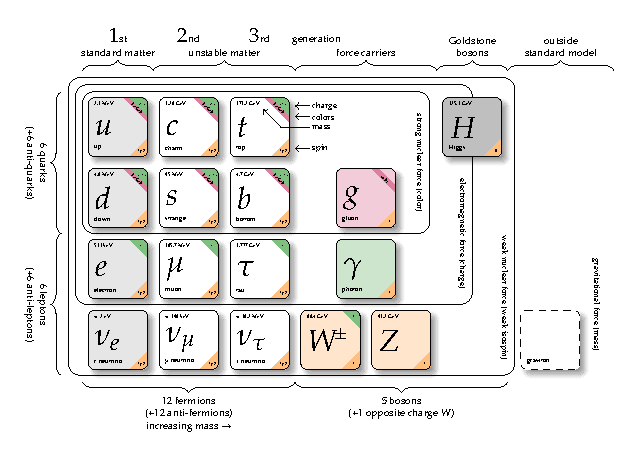
\includegraphics[width=1.0\textwidth]{Fig/model-physics}\\
    \caption{The elementary particles of SM, with the three generations of fermions, four gauge bosons, and the Higgs boson. \label{fig:SMgraph}} 
  \end{center}
\end{figure} 

\subsection{Gauge invariance}
In the context of Quantum Field Theory (QFT), particles are described by excitations of a quantum field which satisfies the quantum field equation. In a continuous system, the \emph{field} represents the generalized coordinates at each point in space-time, and therefore is written in the form of a continuous function. The dynamics of the field is often expressed by the Lagrangian density $\mathcal{L}(\phi_{i},\partial_{\mu}\phi_{i})$ where $\phi_{i}$ is the field. Later in the text a simplified term ''the Lagrangian`` will be used to replace the Lagrangian density.
The equation of motion describing the dynamics of the field can be derived from the Euler-Lagrange equation 
\begin{equation}
\partial_{\mu}\bigg(\frac{\partial\mathcal{L}}{\partial(\partial_{\mu}\phi_{i})}\bigg)-\frac{\partial\mathcal{L}}{\partial\phi_{i}}=0.
\end{equation}

The three interactions, QED, weak, and QCD, can be derived by requiring the \emph{local guage invariance}: the Lagrangian is invariant under the \emph{local phase transformation} of the fields,
\begin{equation}
\psi(x) \ \to\ \psi^{\prime}(x) = \hat{U(x)}\psi(x) = \mathrm{e}^{iq\chi(x)}\psi(x).
\end{equation}
The Lagrangian for a free spin-$\frac{1}{2}$ particle (referred to as free Lagrangian)
\begin{equation}
\label{eqn:LagSpinhalf}
\mathcal{L}_{\text{free}}=i\bar{\psi}\gamma^{\mu}\partial_{\mu}\psi-m\bar{\psi}\psi.
\end{equation}
With the U(1) local gauge transformation, Eq.~\ref{eqn:LagSpinhalf} becomes
\begin{equation}
\label{eqn:LagSpinhalf_LocalTrans}
\mathcal{L}_{\text{free}}\ \to\ \mathcal{L}_{\text{free}}^{\prime} = \mathcal{L}_{\text{free}} - q\bar{\psi}\gamma_{\mu}\big(\partial_{\mu}\chi\big)\psi.
\end{equation}
The free Lagrangian is obviously not invariant under U(1) local gauge transformation. 
The solution to deal with the extra term in Eq.~\ref{eqn:LagSpinhalf_LocalTrans} is to replace the derivative $\partial_{\mu}$ in the free Lagrangian with the \emph{covariant derivative} $D_{\mu}$,
\begin{equation}
\label{eqn:covderivative}
\partial_{\mu}\ \to\ D_{\mu}=\partial_{\mu}+iqA_{\mu},
\end{equation}
with the introduction of a new field $A_{\mu}$. 
After the replacement, the new field $A_{\mu}$ transforms in coordination with the local phase transformation of the $\psi$ as
\begin{equation}
\label{eqn:U1gaugetrans}
A_{\mu}\ \to\ A_{\mu}^{\prime}=A_{\mu}-\partial_{\mu}\chi,
\end{equation}
The invariance of the Lagrangian can be preserved. It is worth noting that Eq.~\ref{eqn:U1gaugetrans} is actually the concept of gauge transformation of the electromagnetic vector potential $A_{\mu}$ in the classical electromagnetism. The requirement of the U(1) local invariance of the Lagrangian takes price, which is to introduce a vector field that couples to the spin-$\frac{1}{2}$ particles. The full Lagrangian should include this newly introduced vector field. The corresponding terms in the Lagrangian is known as the Proca Lagrangian
\begin{equation}
\label{eqn:LagProca}
\mathcal{L}_{\text{Proca}}=-\frac{1}{4}F^{\mu\nu}F_{\mu\nu}+\frac{1}{2}m_{A}^{2}A^{\mu}A_{\mu}.
\end{equation}
where the $F_{\mu\nu}\equiv(\partial_{\mu}A_{\nu}-\partial_{\nu}A_{\mu})$ is the field-strength tensor.
However, the $F_{\mu\nu}$ is invariant under Eq.~\ref{eqn:U1gaugetrans} while the $A^{\mu}A_{\mu}$ term transforms as
\begin{equation}
\frac{1}{2}m_{A}^{2}A^{\mu}A_{\mu}\ \to\ \frac{1}{2}m_{A}^{2}\big(A_{\mu}-\partial_{\mu}\chi\big)\big(A^{\mu}-\partial^{\mu}\chi\big)\neq\frac{1}{2}m_{A}^{2}A^{\mu}A_{\mu},
\end{equation}
which is certainly not invariant. A conclusion can be drawn that the U(1) local gauge symmetry can only be satisfied with the \emph{massless} gauge boson of the interaction.
The Lagrangian describing the QED takes the form
\begin{equation}
\label{eqn:LagQED}
\mathcal{L}_{\text{QED}}=\big(i\bar{\psi}\gamma^{\mu}\partial_{\mu}\psi - m\bar{\psi}\psi\big) - \big(q\bar{\psi}\gamma_{\mu}\psi\big)A_{\mu} -\frac{1}{4}F^{\mu\nu}F_{\mu\nu}.
\end{equation}

The introduction of the new field not only exhibits the observed gauge invariance of classical electromagnetism, but also corresponds to a wave equation with an interaction term of the form 
\begin{equation}
\label{eqn:interactionQED}
q\gamma^{\mu}A_{\mu}\psi.
\end{equation}
This is the QED interaction potential, and its vertex is shown in Fig.~\ref{fig:QEDvtx}.
\begin{figure}[!ht]
  \begin{center}  
    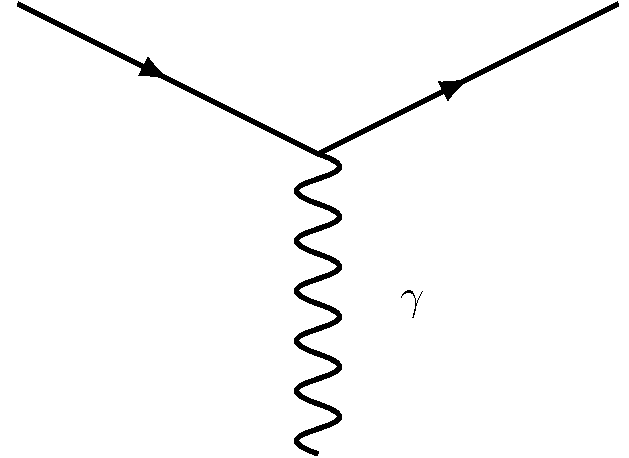
\includegraphics[width=0.25\textwidth]{Fig/QED_vertex}\\
    \caption{The Feynman diagram of the QED vertex. \label{fig:QEDvtx}} 
  \end{center}
\end{figure} 
The requirement of the physics to be invariant under local U(1) phase transformations implies that a gauge field must exist, and the excitation of this field is now commonly identified as the massless gauge boson -- the photon.

The same construction can be applied to the weak and the strong interactions (QCD, quantum chromodynamics), of which the underlying symmetry is the invariance under SU(2) and SU(3) local phase transformations respectively,
\begin{equation}
\label{eqn:SU3transform}
\psi(x) \ \to\ \psi^{\prime}(x) = \exp\bigg[ig_{S}\boldsymbol{\alpha}(x)\cdot\boldsymbol{M}\bigg]\psi(x),
\end{equation}
with the corresponding replacements of the partial derivatives to covariant derivatives,
\begin{equation}
\label{eqn:covderivative_SU23}
\partial_{\mu}\ \to\ D_{\mu}=\partial_{\mu}+ig_{W(S)}\boldsymbol{M}\cdot \boldsymbol{G}_{\mu}(x),
\end{equation}
where $g_{W(S)}$ is the coupling constant of weak (strong) interaction, $\boldsymbol{M}$ are the generators of SU(2) (SU(3)) symmetry group, and $\boldsymbol{G}$ are the three (eight) new gauge fields of weak (stron) interaction.
The well-known representations of the SU(2) group are the Pauli matrices and of the SU(3) are the Gell-Mann matrices.

In the following paragraphs, the weak interaction will be introduced a bit deeper.

\subsection{Weak interaction and the electroweak unification}
The weak interaction at first was proposed to explain the beta decay. Fermi (1933) treated the process as a contact interaction, which takes place at a single space-time point and does not require mediating particles. Nowadays, it is widely known that the Fermi's model is the low energy approximation and will fail at high energy regime. 

At the beginning, this theory only includes the charged-current weak interaction which can be associated with invariance under SU(2) local phase transformation
\begin{equation}
\label{eqn:SU2transform}
\psi(x) \ \to\ \psi^{\prime}(x) = \exp\bigg[ig_{W}\boldsymbol{\chi}(x)\cdot\boldsymbol{M}\bigg]\psi(x),
\end{equation}
where $\boldsymbol{M}$ are the three generators of the SU(2) symmetry group, of which the representation is the Pauli matrix,
\begin{equation}
\boldsymbol{M}=\frac{1}{2}\boldsymbol{\sigma}.
\end{equation}
The local guage invariance is satisfied with the three introduced fields, $W_{\mu}^{k}$ with $k=1,2,3$, corresponding to three gauge bosons $W^{(1)}$, $W^{(2)}$, and $W^{(3)}$. Since the SU(2) generators are represented by $2\times2$ matrices, the wavefunction must have two additional degrees of freedom. 
Furthermore, only left-handed (LH) chiral particles and right-handed (RH) chiral antiparticles couple to the weak charged-current interaction, LH particles and RH antiparticles are placed in weak isospin doublets. On the other hand, RH particles and LH antiparticles are put into weak isospin singlets and hence will not be affected by the transformation of Eq.~\ref{eqn:SU2transform}. Consequently, the wave functions can be interpreted as 
\begin{equation}
\label{eqn:WeakWaveFunc}
\psi(x) = \binom{\mu_{i}}{\ell_{i}}_{L},\ \binom{u_{i}}{d_{i}}_{L},\ (u_{i})_{R},\ (d_{i})_{R},\ (\ell_{i})_{R},
\end{equation}
where $i = 1, 2, 3$ for the three families of fermions.
Again, the requirement of the local gauge invariance necessitates the modification of the Dirac equation to include a new interaction term 
\begin{equation}
\label{eqn:WeakInteraction}
ig_{W}T_{k}\gamma^{\mu}W_{\mu}^{k}\psi_{L}=ig_{W}\frac{1}{2}\sigma_{k}\gamma^{\mu}W_{\mu}^{k}\psi_{L},
\end{equation}
where $\psi_{L}$ stands for the weak isospin doublet of LH particles. 
From this form of interaction, three weak currents can be associated with Pauli matrices,
\begin{equation}
\label{eqn:WeakCurrent1}
j_{1}^{\mu}=\frac{g_{W}}{2}\bar{\psi}_{L}\gamma^{\mu}\sigma_{i}\psi_{L},
\end{equation}
where $i=1,2,3$. The actual charged-currents relate to the isospin raising the lowering operators, $\sigma_{\pm}=\frac{1}{2}(\sigma_{1}\pm i\sigma_{2})$, and read as 
\begin{equation}
\label{eqn:WeakCurrent2}
j_{\pm}^{\mu}=\frac{1}{\sqrt{2}}\bigg(j_{1}^{\mu}\pm ij_{2}^{\mu}\bigg)=\frac{g_{W}}{\sqrt{2}}\bar{\psi}_{L}\gamma^{\mu}\sigma_{\pm}\psi_{L}.
\end{equation}
In the case of the doublet formed by the LH electron and electron neutrino, the currents $j_{\pm}^{\mu}$, corresponding to the exchange of the physical $\Wpm$ bosons, are
\begin{equation}
\label{eqn:WeakCurrent3}
j_{+}^{\mu}=\frac{g_{W}}{\sqrt{2}} \big(\bar{\nu}_{L}\ \bar{\Pe}_{L}\big) \gamma^{\mu} \begin{pmatrix}
  0 & 1 \\
  0 & 0 
 \end{pmatrix}
 \binom{\nu_{l}}{\Pe_{L}} = \frac{g_{W}}{\sqrt{2}}\bar{\nu}\gamma^{\mu} \frac{1}{2}(1-\gamma^{5})e,
\end{equation}
\begin{equation}
\label{eqn:WeakCurrent4}
j_{-}^{\mu}=\frac{g_{W}}{\sqrt{2}} \big(\bar{\nu}_{L}\ \bar{\Pe}_{L}\big) \gamma^{\mu} \begin{pmatrix}
  0 & 0 \\
  1 & 0 
 \end{pmatrix}
 \binom{\nu_{l}}{\Pe_{L}} = \frac{g_{W}}{\sqrt{2}}\bar{e}\gamma^{\mu} \frac{1}{2}(1-\gamma^{5})\nu,
\end{equation}
consistent with the experimental observation of the vector minus axial vector (V-A) structure.
The physical $\PW$ bosons are identified as
\begin{equation}
\label{eqn:Wboson}
\Wpm_{\mu}=\frac{1}{\sqrt{2}}\bigg(\PW_{\mu}^{(1)}\mp i\PW{\mu}^{(2)}\bigg).
\end{equation}

The $\text{SU(2)}_{L}$ does not only give two weak charged-currents, but also implies the existence of a weak neutral-current
\begin{equation}
\label{eqn:WeakNeuCur}
j_{3}^{\mu}=g_{W}\bar{\psi}_{L}\gamma^{\mu}\frac{1}{2}\sigma_{3}\psi_{L}.
\end{equation}
In the case of the fermion doublet (again, the LH electron and electron neutrino are used as an example), it reads as
\begin{equation}
\label{eqn:WeakCur5}
j_{3}^{\mu}=g_{W}\frac{1}{2} \big(\bar{\nu}_{L}\ \bar{\Pe}_{L}\big) \gamma^{\mu} \begin{pmatrix}
  1 & 0 \\
  0 & -1 
 \end{pmatrix}
 \binom{\nu_{l}}{\Pe_{L}} = g_{W}\frac{1}{2} \bar{\nu}_{L}\gamma^{\nu}_{L} - g_{W}\frac{1}{2} \bar{\Pe}_{L}\gamma^{\mu}\Pe_{L}
\end{equation}
or in a more compact form
\begin{equation}
\label{eqn:WeakCur6}
j_{3}^{\mu}=I_{W}^{(3)}g_{W}\bar{f}\gamma^{\mu} \frac{1}{2} (1-\gamma^{5}) f,
\end{equation}
where $f$ represents the fermion doublet and $I_{W}^{(3)}$ is the third component of the weak isospin. 
The property that RH particles and LH antiparticles do not couple to the weak interaction is perserved, as they possess $I_{W}^{(3)}=0$.
(One should not mix this weak neutral-current with the SM $\cPZ$ boson that currently known, as the reason will be stated in the following paragraphs.)

There is another evidence and argument that the weak neutral-current must exist: the cross-section of the $\PW$ boson pair production in the electron-positron collisions do not converge if there is no neutral-current interaction. Fig.~\ref{fig:eeWWDiagrams} shows the leading order diagrams of the $\EE\to\PWp\PWm$ process. The left most diagram is the charged-current process. The middle one is the electromagnetic process as it is mediated by the photon, and there is also a $\gamma\PW\PW$ vertex indicating that the $\gamma$ can couple with $\PW$ boson since they carry electric charge. In the right most diagram, a neutral boson, which is now known as the $\cPZ$ boson, acts as the mediator. 
Fig.~\ref{fig:eeWWUnitarity} shows the predicted $\EE\to\PWp\PWm$ cross-sections of three cases: only the $\nu_{e}$ diagram included; only $\nu_{e}$ and $\gamma$ diagrams included; all diagrams included~\cite{Schael:2013ita}. With only the first two diagrams, the cross-section will increase without limit. The inclusion of the neutral-current interaction makes the calculated cross-section converge and consistent with the experimental observation. 
\begin{figure}[!ht]
  \begin{center}  
    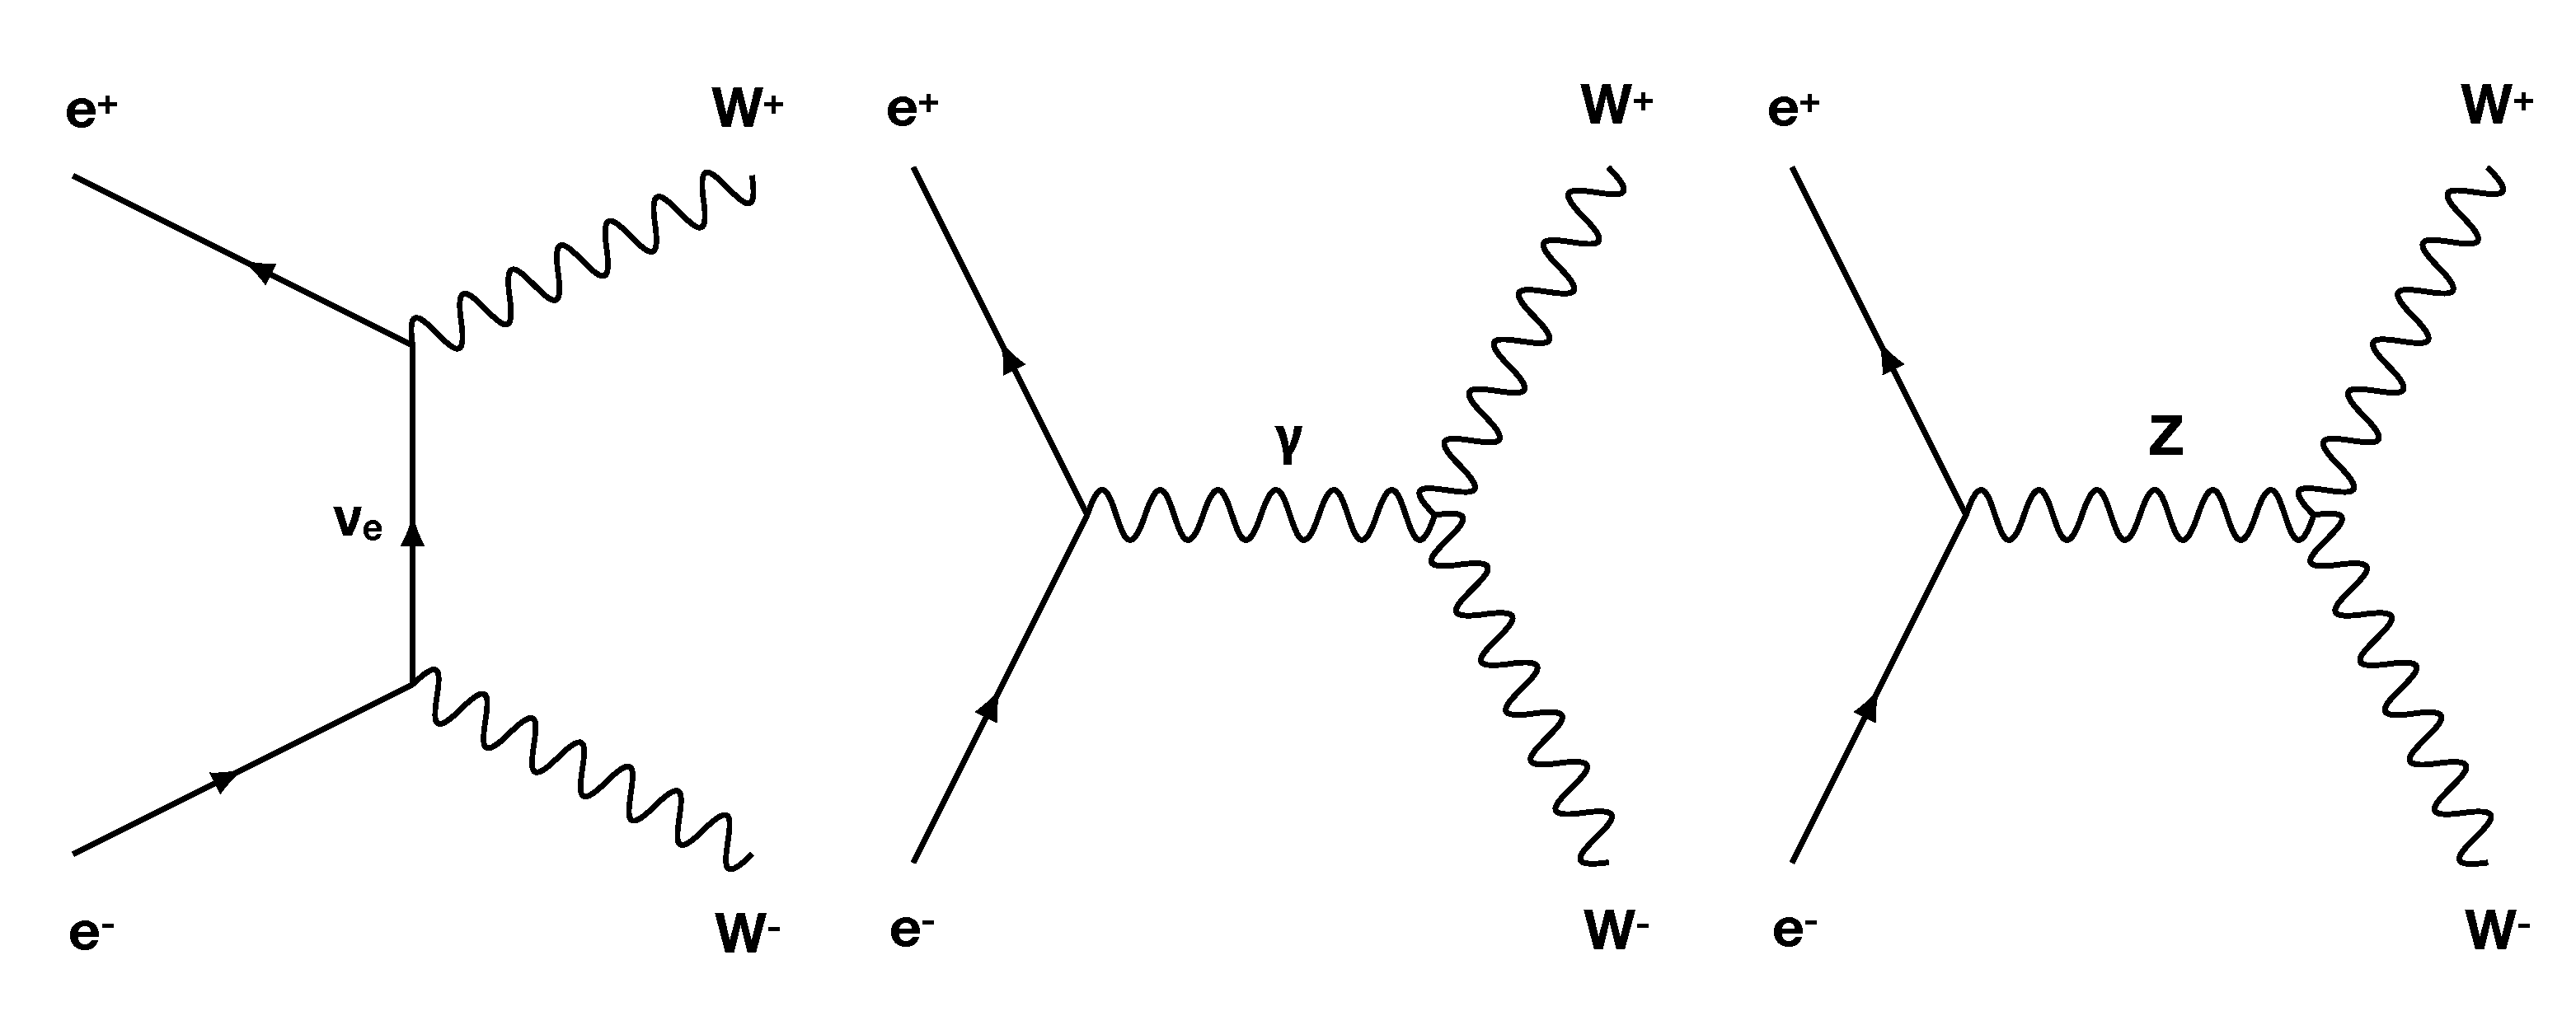
\includegraphics[width=0.8\textwidth]{Fig/eeWW}
    \caption{The leading order diagrams of the $\EE\to\PWp\PWm$ process. \label{fig:eeWWDiagrams}} 
  \end{center}
\end{figure}

\begin{figure}[!ht]
  \begin{center}  
    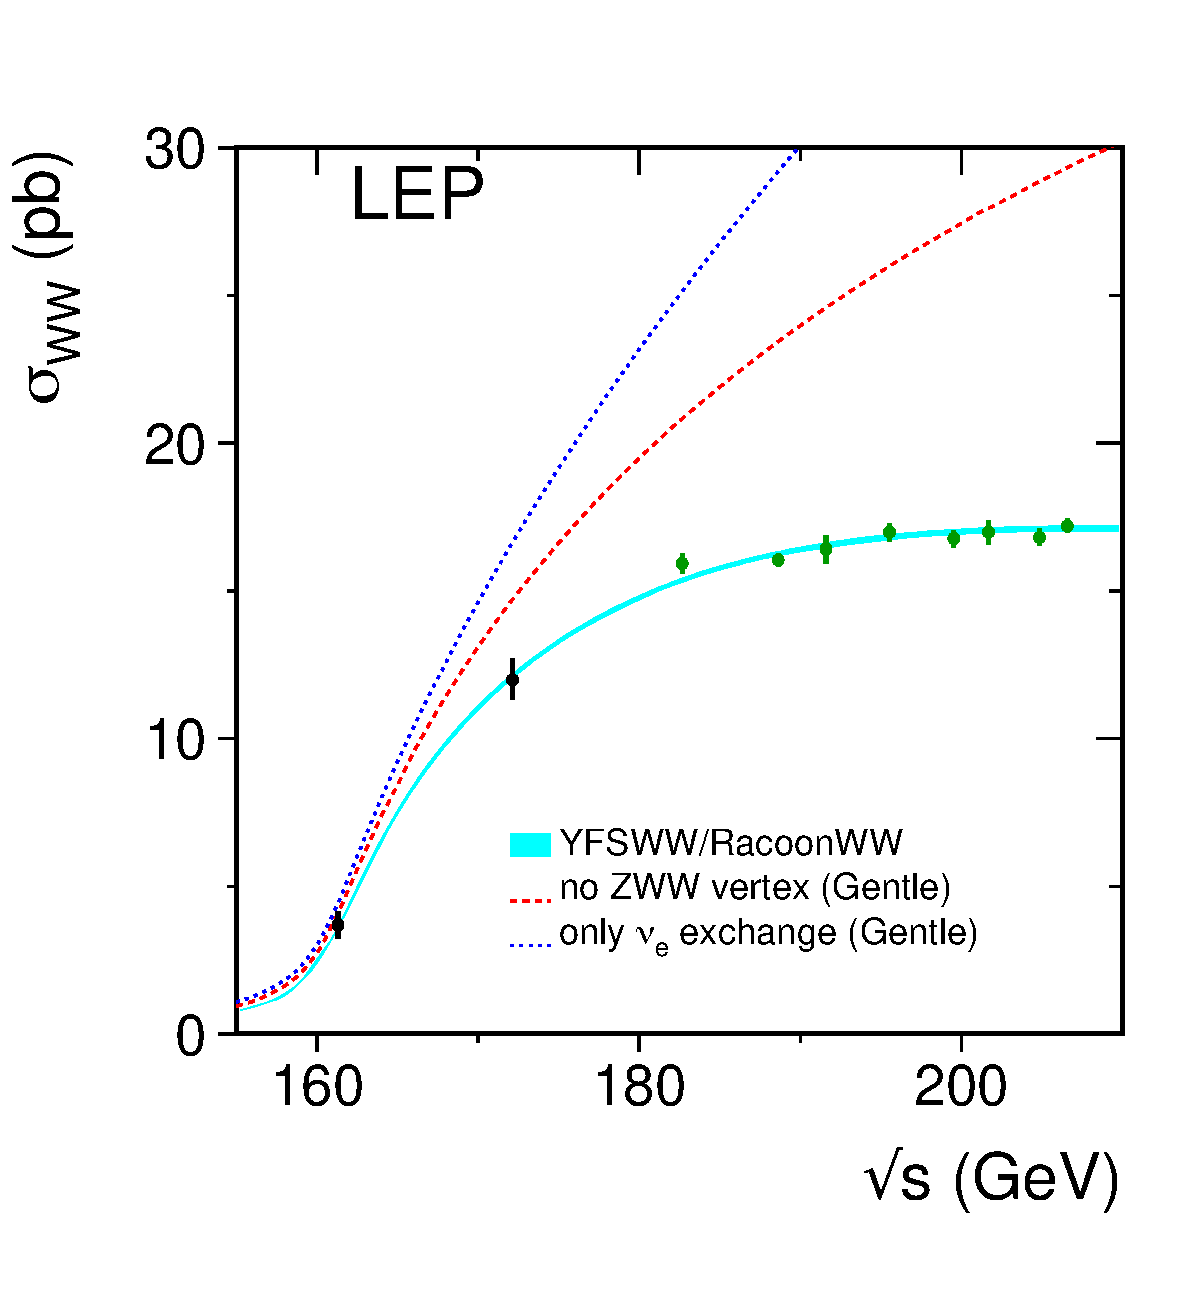
\includegraphics[width=0.6\textwidth]{Fig/4f_wwxsec_nocouplings_2008}
    \caption{Measurements of the $\PW$-pair production cross-section, compared to the different predictions. The shaded area represents the uncertainty on the theoretical predictions~\cite{Schael:2013ita}. \label{fig:eeWWUnitarity}} 
  \end{center}
\end{figure} 

The cancellation that preserves the unitary of $\EE\to\PWp\PWm$ indicates that the coupling of the $\gamma$, charged- and neutral-currents are related. A unification of the electromagnetic and weak interaction was proposed, and a unified electroweak model was completed by Sheldon Glashow, Abdus Salam, and Steven Weinberg, and now it is called GSW model.

One thing that must be incorporated in the unification is the correspondence between the weak neutral-current and the physical $\cPZ$ boson. The neutral-current previously stated does not couple to RH particles/LH antiparticles, which is in contrast to the experimental evidence that the neutral $\cPZ$ boson couples, not equally, to both LH and RH particles. 
At the first step, a $\text{U(1)}_{Y}$ local gauge symmetry is introduced to replace the U(1) gauge group of the electromegnetism with the transformation
\begin{equation}
\psi(x) \ \to\ \psi^{\prime}(x) = \hat{U(x)}\psi(x) = \exp\bigg[ig^{\prime}\frac{Y}{2}\chi^{\prime}(x)\bigg]\psi(x),
\end{equation}
with a new field $B_{\mu}$ and a new weak hypercharge $Y$.
This new symmetry yields the same interaction term as the U(1) symmetry of the QED in Eq.~\ref{eqn:interactionQED}, 
\begin{equation}
\label{eqn:IntactionHyper}
g^{\prime}\frac{Y}{2}\gamma^{\mu}B_{\mu}\psi.
\end{equation}
The physical photon $\gamma$ and $\cPZ$ boson are expressed as,
\begin{equation}
\label{eqn:Afield}
A_{\mu}=+B_{\mu}\cos\theta_{W} + W_{\mu}^{(3)}\sin\theta_{W},
\end{equation}
\begin{equation}
\label{eqn:Zfield}
Z_{\mu}=-B_{\mu}\sin\theta_{W} + W_{\mu}^{(3)}\cos\theta_{W},
\end{equation}
where the $\theta_{W}$ is the weak mixing angle. The physical QED and weak neutral- current are therefore,
\begin{equation}
\label{eqn:jem1}
j_{em}^{\mu}=j_{Y}^{\mu}\cos\theta_{W} + j_{3}^{\mu}\sin\theta_{W},
\end{equation}
\begin{equation}
\label{eqn:jz1}
j_{Z}^{\mu}=-j_{Y}^{\mu}\sin\theta_{W} + j_{3}^{\mu}\cos\theta_{W},
\end{equation}
with the weak neutral-current $j_{3}$ of Eq.~\ref{eqn:WeakCur5} and the current associated with the interaction term $j_{Y}$ of Eq.~\ref{eqn:IntactionHyper} 
\begin{equation}
j_{Y}^{\mu}=\frac{1}{2}g^{\prime}Y_{\Pe_{L}}\bar{\Pe}_{L}\gamma^{\mu}\Pe_{L}
+\frac{1}{2}g^{\prime}Y_{\Pe_{R}}\bar{\Pe}_{R}\gamma^{\mu}\Pe_{R}
+\frac{1}{2}g^{\prime}Y_{\nu_{L}}\bar{\nu}_{L}\gamma^{\mu}\nu_{L}
+\frac{1}{2}g^{\prime}Y_{\nu_{R}}\bar{\nu}_{R}\gamma^{\mu}\nu_{R}
\end{equation}
On the other hand, the electromagnetic current (of the electron doublet) is simply 
\begin{equation}
\label{eqn:jem2}
j_{em}^{\mu}=Q_{e}e\bar{\Pe}_{L}\gamma^{\mu}\Pe_{L}+Q_{e}e\bar{\Pe}_{R}\gamma^{\mu}\Pe_{R}.
\end{equation}
The underlying symmetry group of the electroweak sector, as described in GSW model, is $U(1)_{Y} \times SU(2)_{L}$. In order to preserve the invariance under $U(1)_{Y}$ and $SU(2)_{U}$ local gauge transformation, the hypercharges of particles in a weak isospin doublet should be the same.
Having this argument and equating each component of the Eq.~\ref{eqn:jem1} with $j_{3}^{\mu}$ and $j_{Y}^{\mu}$ substituted and Eq.~\ref{eqn:jem2}, the weak hypercharge can be expressed as a linear combination of the electromagnetic charge $Q$ and the third component of weak isospin $I_{W}^{(3)}$
\begin{equation}
\label{eqn:YQI}
Y=2\big(Q-I_{W}^{(3)}\big),
\end{equation}
Relations between the weak coupling $g_{W}$, the hypercharge coupling $g^{\prime}$ and the electric charge can be derived
\begin{equation}
\label{eqn:relation3}
e=g_{W}\sin\theta_{W}=g^{\prime}\cos\theta_{W}.
\end{equation}
The GSW model successfully bridges the couplings of QED, weak, and the hypercharge with the simple relation.
The measurement of the weak mixing angle, in convention, provides the value of $\sin^{2}\theta_{W}$, which is also the ratio of the weak to electromagnetic coupling constant
\begin{equation}
\label{eqn:relation4}
\sin^{2}\theta_{W}=\frac{\alpha}{\alpha_{W}}=\frac{e^{2}}{g^{2}_{W}}\sim 0.23.
\end{equation}
The coupling of the physical $\cPZ$ boson can be determined similarly. 
From Eq.~\ref{eqn:jz1}, the current of the interaction between the $\cPZ$ boson and a fermion (with flavor $f$) can be written as 
\begin{equation}
\label{eqn:currentZff}
\begin{split}
j_{Z}^{\mu} & = g_{Z}\big(I_{W}^{(3)}-Q_{f}\sin^{2}\theta_{W}\big)\bar{u}_{L}\gamma^{\mu}u_{L}-g_{Z}\big(Q_{f}\sin^{2}\theta_{W}\big)\bar{u}_{R}\gamma^{\mu}u_{R}\\
& \equiv g_{Z}\big(c_{L}\bar{u}_{L}\gamma^{\mu}u_{L}+c_{R}\bar{u}_{R}\gamma^{\mu}u_{R}\big) \\
\end{split}
\end{equation}
where $u_{L(R)}$ is the spinor of LH (RH) states, $c_{L}=I_{W}^{(3)}-Q_{f}\sin^{2}\theta_{W}$ and $c_{R}=-Q_{f}\sin^{2}\theta_{W}$ indicating the strengths of the coupling, and the coupling of the physical $\cPZ$ boson defined as
\begin{equation}
\label{eqn:couplingZ}
g_{Z}=\frac{g_{W}}{\cos\theta_{W}}=\frac{e}{\sin\theta_{W}\cos\theta_{W}}.
\end{equation}
As stated previously, the physical $\cPZ$ boson does couple to LH and RH particles, however, unequally. This is intuitively reasonable, as the current associated with the $\cPZ$ boson is the mixture of the weak and $\text{U(1)}_{Y}$ interactions, where the former one couples only to LH particles but the latter one equally couples to LH and RH particles.

In 1967, Steven Weinberg obtained the formula for the $\PW$ and $\cPZ$ boson masses~\cite{PhysRevLett.19.1264}, with the $\theta_{W}$ which had not yet been determined then. In the following years, the $\theta_{W}$ was measured in various experiments, and in 1982 the masses of the $\PW$ and $\cPZ$ bosons were predicted to be $m_{\PW}=82\pm 2\GeVcc$ and $m_{\cPZ}=92\pm 2 \GeVcc$. In 1983, Carlos Rubbia and his group discovered the $\PW$ and the $\cPZ$ boson~\cite{ARNISON1983103,ARNISON1984241} with measured masses $m_{\PW}=80.403\pm 0.029\GeVcc$ and $m_{\cPZ}=91.188\pm 0.002\GeVcc$. Experiments later on also confirmed the couplings. The GSW model is now considered as one of the most important successes in the SM. 

Despite the triumph of the electroweak unification, it did have some questions regarding the whole mechanism. First of all, Eq.~\ref{eqn:Afield} and \ref{eqn:Zfield} demonstrate that the fields of $U(1)_{Y}$ and $SU(2)_{L}$ are mixed to give physical bosons. The underlying nature of this mixture was unclear. Secondly, four electroweak gauge bosons have different masses, especially when comparing the photon with other three massive particles. This fact seems to contradict the physical picture that both electromagnetic and weak interactions are manifestations of a more fundamental electroweak interaction. The problem with the masses happens also on the fermions. In Eq.~\ref{eqn:LagQED}, the mass term in the QED Lagrangian can be expressed in the chiral states
\begin{equation}
\label{eqn:FermionMass_QEDLag}
\begin{split}
-m\bar{\psi}\psi & = -m\bar{\psi}\bigg[\frac{1}{2}(1-\gamma^{5})+\frac{1}{2}(1+\gamma^{5})\bigg]\psi \\
& = -m\bar{\psi}\bigg[\frac{1}{2}(1-\gamma^{5})\psi_{L}+\frac{1}{2}(1+\gamma^{5})\psi_{R}\bigg] \\
& = -m\big(\bar{\psi}_{R}\psi_{L}+\bar{\psi}_L\psi_{R}\big). 
\end{split}
\end{equation}
In the $\text{SU(2)}_{L}$ gauge transformation of the weak interaction, LH particles transform as doublets while RH particles as singlets. Eq.~\ref{eqn:FermionMass_QEDLag} obviously does not follow the required gauge invariance.
Thirdly, a problem was found: the unitarity violation of the scattering process $\PWp\PWm\to\PWp\PWm$. An overview of the $\PW\PW$ scattering process can be found in Ref.~\cite{Szleper:2014xxa}. The original calculation for the amplitude included the diagrams, shown in Fig.~\ref{fig:WWWWscattering1}. The unitarity violation results from the longitudinal polarized states of $\PW$ boson and the process $\PW_{L}\PW_{L}\to\PW_{L}\PW_{L}$. The issue is solved by introducing a new scalar particle to mediate the $\PW\PW$ process. The diagrams are shown in Fig.~\ref{fig:WWWWscattering_Higgs}.
All the above three problems necessitate a new mechanism, which is now called the Higgs mechanism, with its manifestation, the Higgs boson. 
\begin{figure}[!ht]
  \begin{center}  
    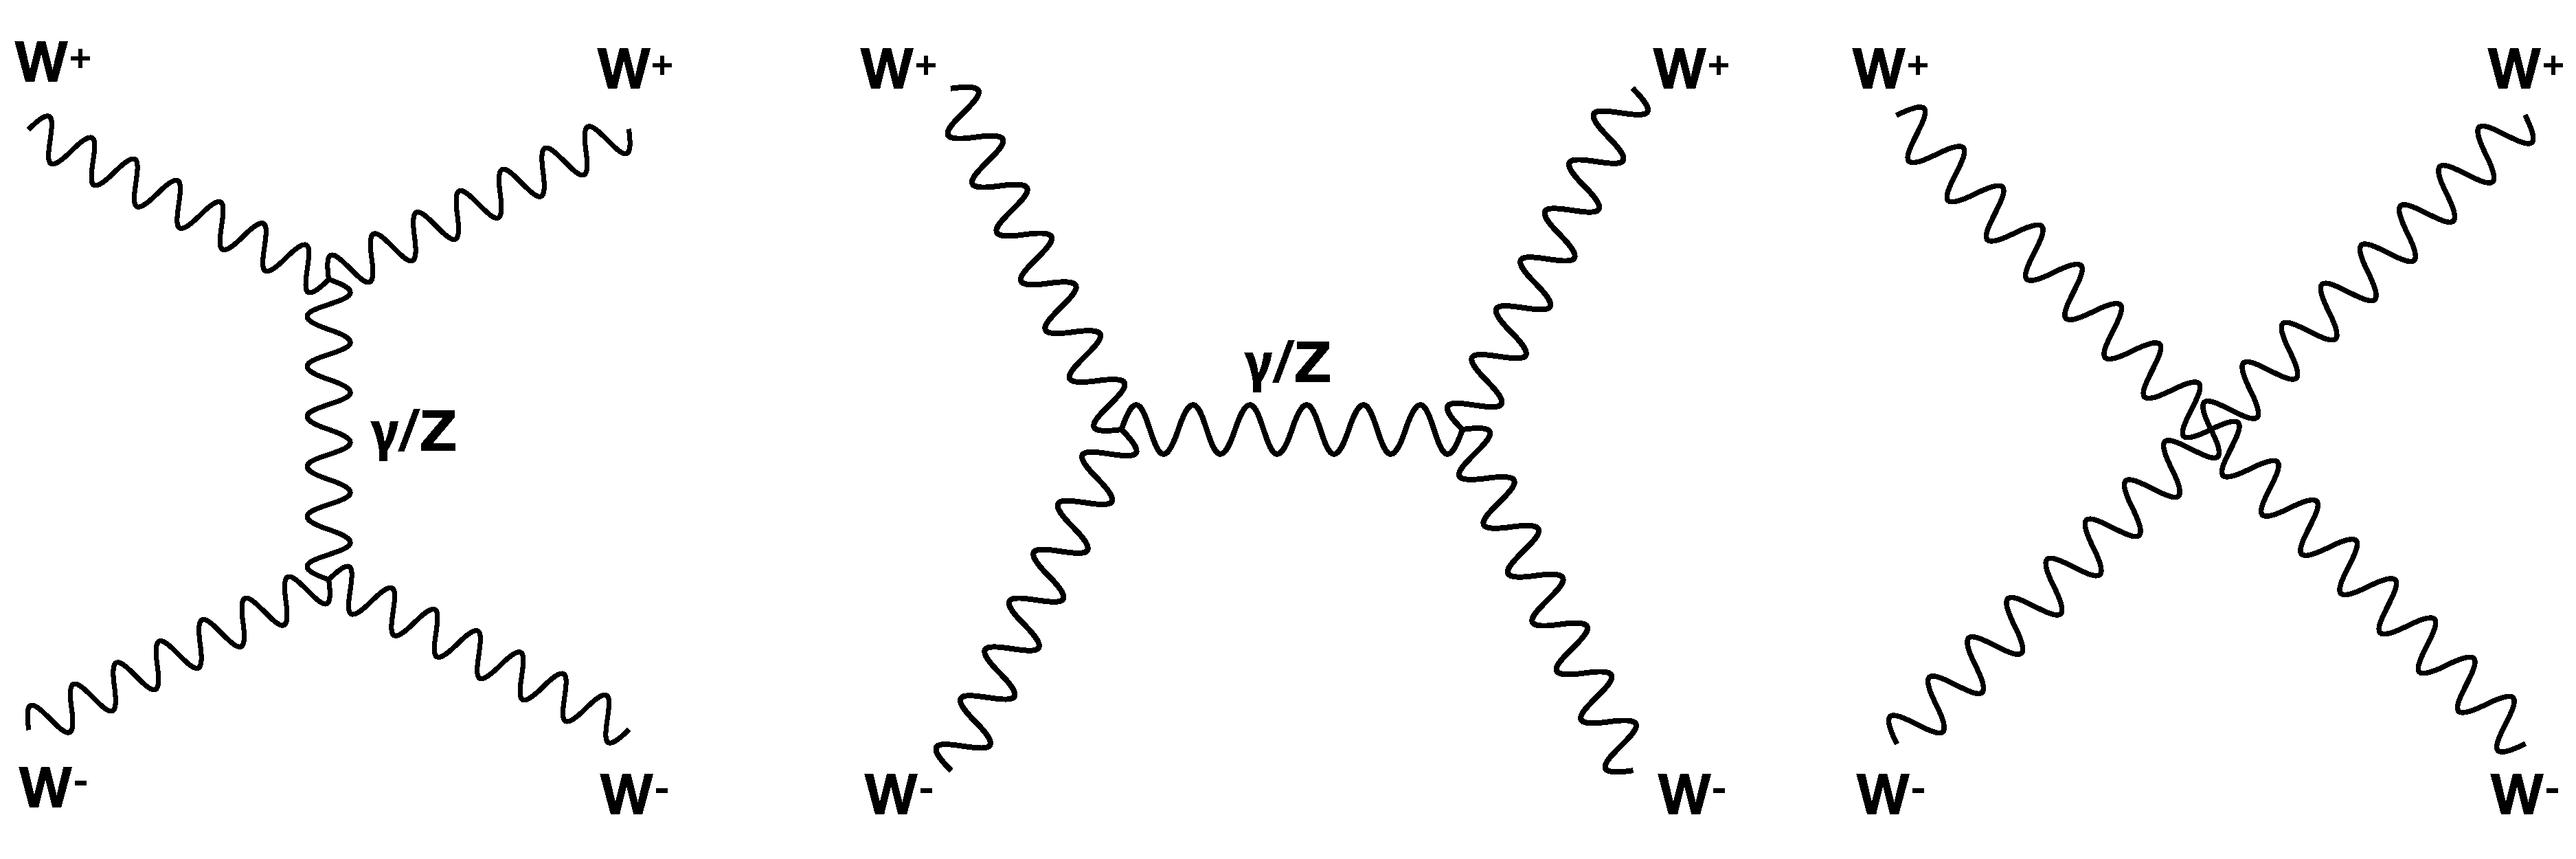
\includegraphics[width=0.67\textwidth]{Fig/WWWWscattering}\\
    \caption{The leading order diagrams for $\PWp\PWm\to\PWp\PWm$ scattering process. \label{fig:WWWWscattering1}}  
  \end{center}
\end{figure}

\begin{figure}[!ht]
  \begin{center}  
    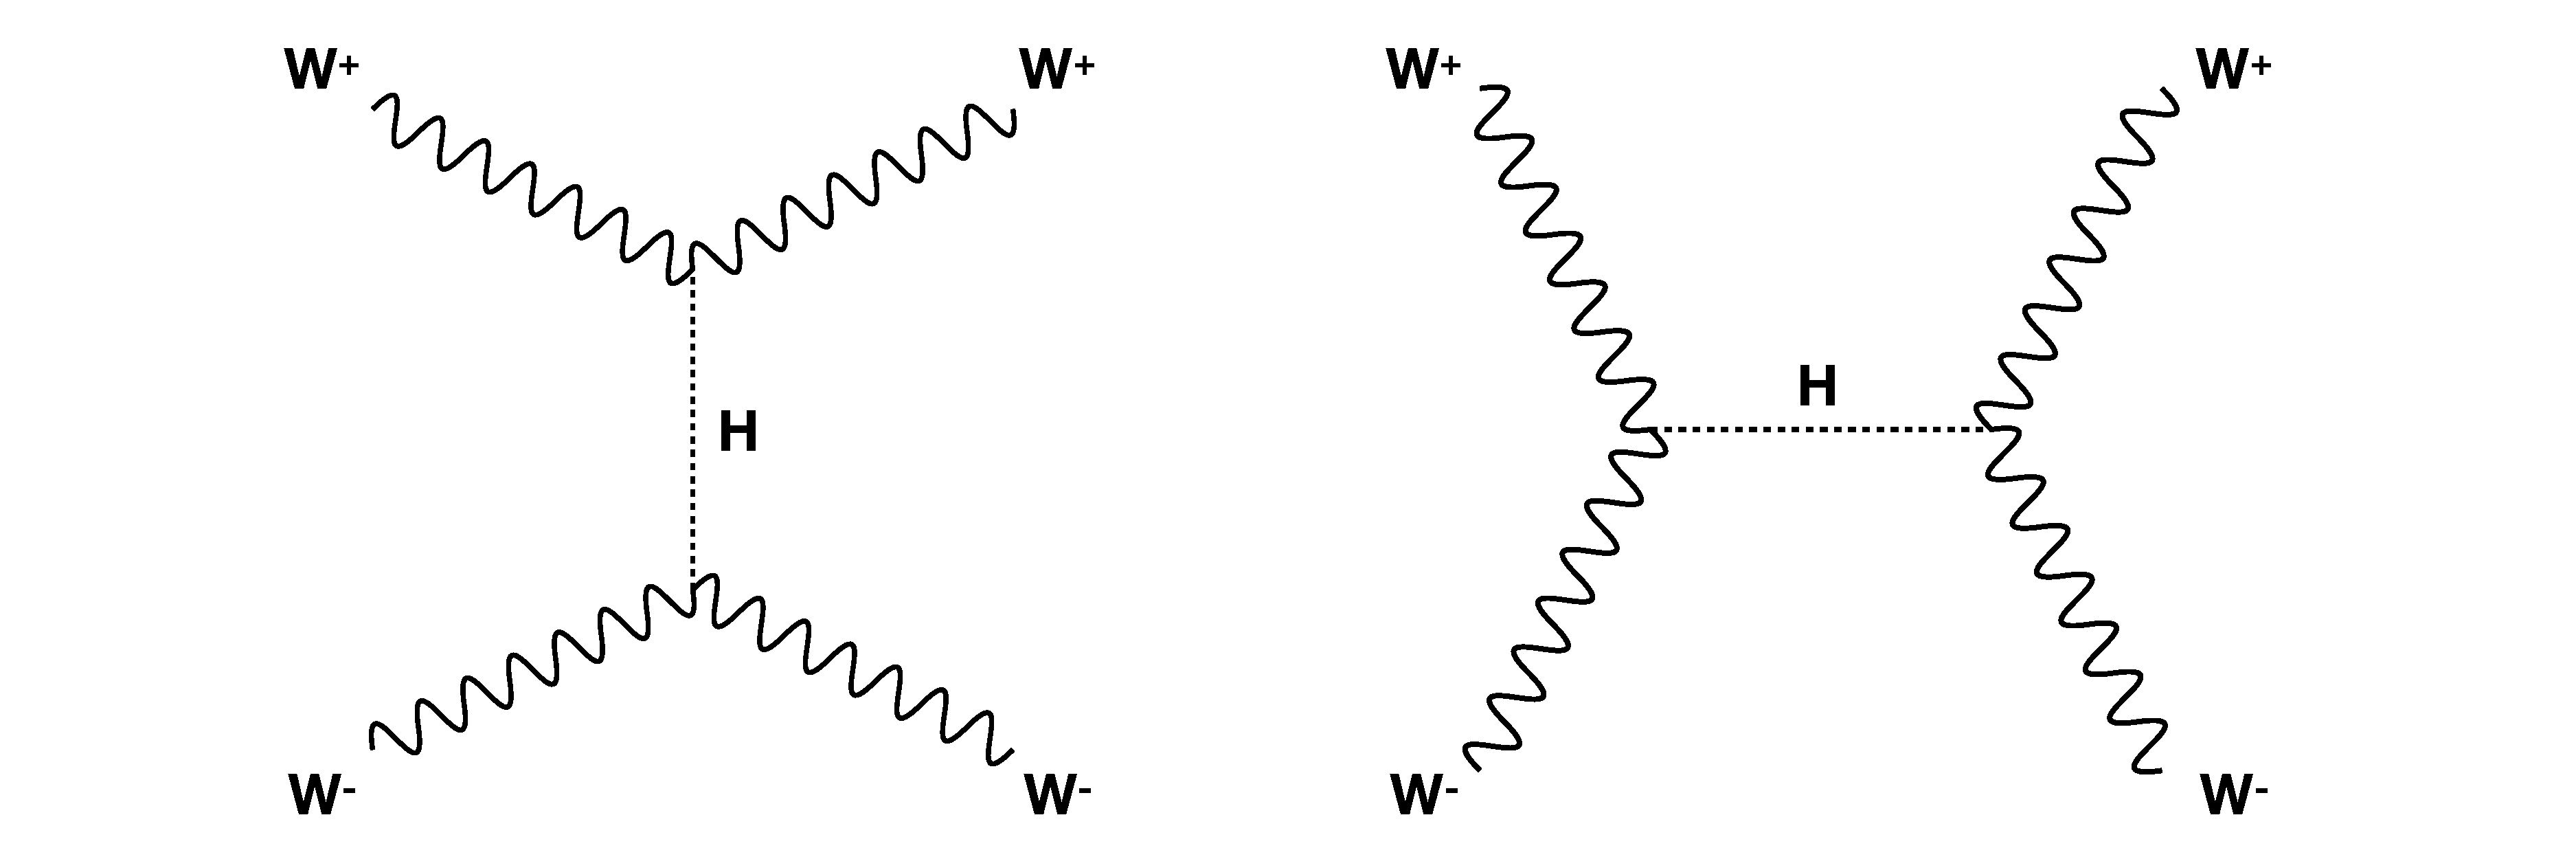
\includegraphics[width=0.67\textwidth]{Fig/WWWWscattering_Higgs}\\
    \caption{The diagrams for $\PWp\PWm\to\PWp\PWm$ scattering process with a scalar boson as mediator. \label{fig:WWWWscattering_Higgs}}  
  \end{center}
\end{figure}

\subsection{The Higgs mechanism}
The Higgs mechanism was proposed back to 1964 by Robert Brout and François Englert, Peter Higgs, and Gerald Guralnik, C. R. Hagen, and Tom Kibble~\cite{PhysRevLett.13.321,PhysRevLett.13.508,PhysRevLett.13.585}.

Before formally introducing the Higgs mechanism in the SM, a single scalar field $\phi$ is used as an example to illustrate the concept. Consider the potential of the form
\begin{equation}
V(\phi) = \frac{1}{2}\mu^{2}\phi^{2} + \frac{1}{4}\lambda\phi^{4}.
\end{equation}
The corresponding Lagrangian is given by 
\begin{equation}
\begin{split}
\mathcal{L}_{ex} & = \frac{1}{2}(\partial_{\mu}\phi)(\partial^{\mu}\phi)- V(\phi) \\
& = \frac{1}{2}(\partial_{\mu}\phi)(\partial^{\mu}\phi) - \frac{1}{2}\mu^{2}\phi^{\mu} - \frac{1}{4}\lambda\phi^{4}.
\end{split}
\end{equation}
In this example Lagrangian, the term of $(\partial_{\mu}\phi)(\partial^{\mu}\phi)$ can be associated with the kinematic energy of the scalar particle. The term of $\phi^{2}$ can be read as the mass of the particle (strictly to say, when $\mu^{2}>0$, it is the coefficient of the $\phi^{2}$ term that associates to the mass). The $\phi^{4}$ term is identified as self-interactions of the scalar field.

The vacuum state is the lowest energy state of the field. In the field theory, the particles state (or the excitations of the field) can be obtained by applying perturbations of the field around the vacuum state. 
In order to have minima for the potential, the $\lambda$ must be positive. When $\mu^{2}>0$, the minimum of the potential happens to be at $\phi=0$. When $\mu^{2}<0$, the term can no longer be interpreted as mass, and the potential now has two degenerate minima at $\phi=\pm v=\pm \mid \sqrt{\frac{-\mu^{2}}{\lambda}} \mid$. 
One needs to arbitrarily select one of the degenerate states as the ground state, then the ground state no longer preserves the symmetry of the Lagrangian. This way to obtain the asymmetric vacuum state is known as \emph{spontaneous symmetry breaking}.

In the SM, the Higgs mechanism is embedded in the $\text{U(1)}_{Y}\times\text{SU(2)}_{L}$ local gauge symmetry of the electroweak sector.
As the Higgs mechanism is required to generate masses of the electroweak gauge bosons, one of the scalar fields must be neutral (therefore termed as $\phi^{0}$), and the other must be charged ($\phi^{+}$ and $\phi^{-}=(\phi^{+})^{\ast}$) to give the longitudinal polarization states of the $\PW$ bosons\footnotemark.
\footnotetext{Before the Higgs mechanism, the gauge bosons do not have masses. Hence, they can only have transverse polarization states. After acquiring the masses, gauge bosons become massive particles, which can have longitudinal polarization state.}
The simplest Higgs model, which has four degrees of freedom and consists of two complex scalar fields, is placed in a weak isospin doublet, 
\begin{equation}
\label{eqn:HiggsModel}
\phi=\begin{pmatrix}
  \phi^{+} \\
  \phi^{0}  
 \end{pmatrix}
 =\frac{1}{\sqrt{2}}\begin{pmatrix}
  \phi_{1}+i\phi_{2} \\
  \phi_{3}+i\phi_{4}  
 \end{pmatrix}
 .
\end{equation}
The Lagrangian of this doublet of fields is 
\begin{equation}
\label{eqn:Lagrangian_Higgs}
\mathcal{L}=(\partial_{\mu}\phi)^{\dagger}(\partial^{\mu}\phi) - V(\phi),
\end{equation}
To preserve the invariance under the $\text{U(1)}_{Y}\times\text{SU(2)}_{L}$ local gauge transformation, the derivative in the Lagrangian should be replaced by the covariant derivative of the form
\begin{equation}
\label{eqn:covderivative_Higgs}
\partial_{\mu}\ \to\ D_{\mu}=\partial_{\mu}+ig_{W}\boldsymbol{T}\cdot\boldsymbol{W}_{\mu}+ig^{\prime}\frac{Y}{2}B_{\mu},
\end{equation}
where $\boldsymbol{T}=\frac{1}{2}\sigma$ are the three generators of the SU(2) group.
The Higgs potential is of the form
\begin{equation}
\label{eqn:Higgspotential}
V(\phi) = \mu^{2}\phi^{\dagger}\phi + \lambda(\phi^{\dagger}\phi)^{2},
\end{equation}
where $\lambda$ is positive.
The visualization of the Higgs field is shown in Fig.~\ref{fig:HiggsPotential}.
\begin{figure}[!ht]
  \begin{center}  
    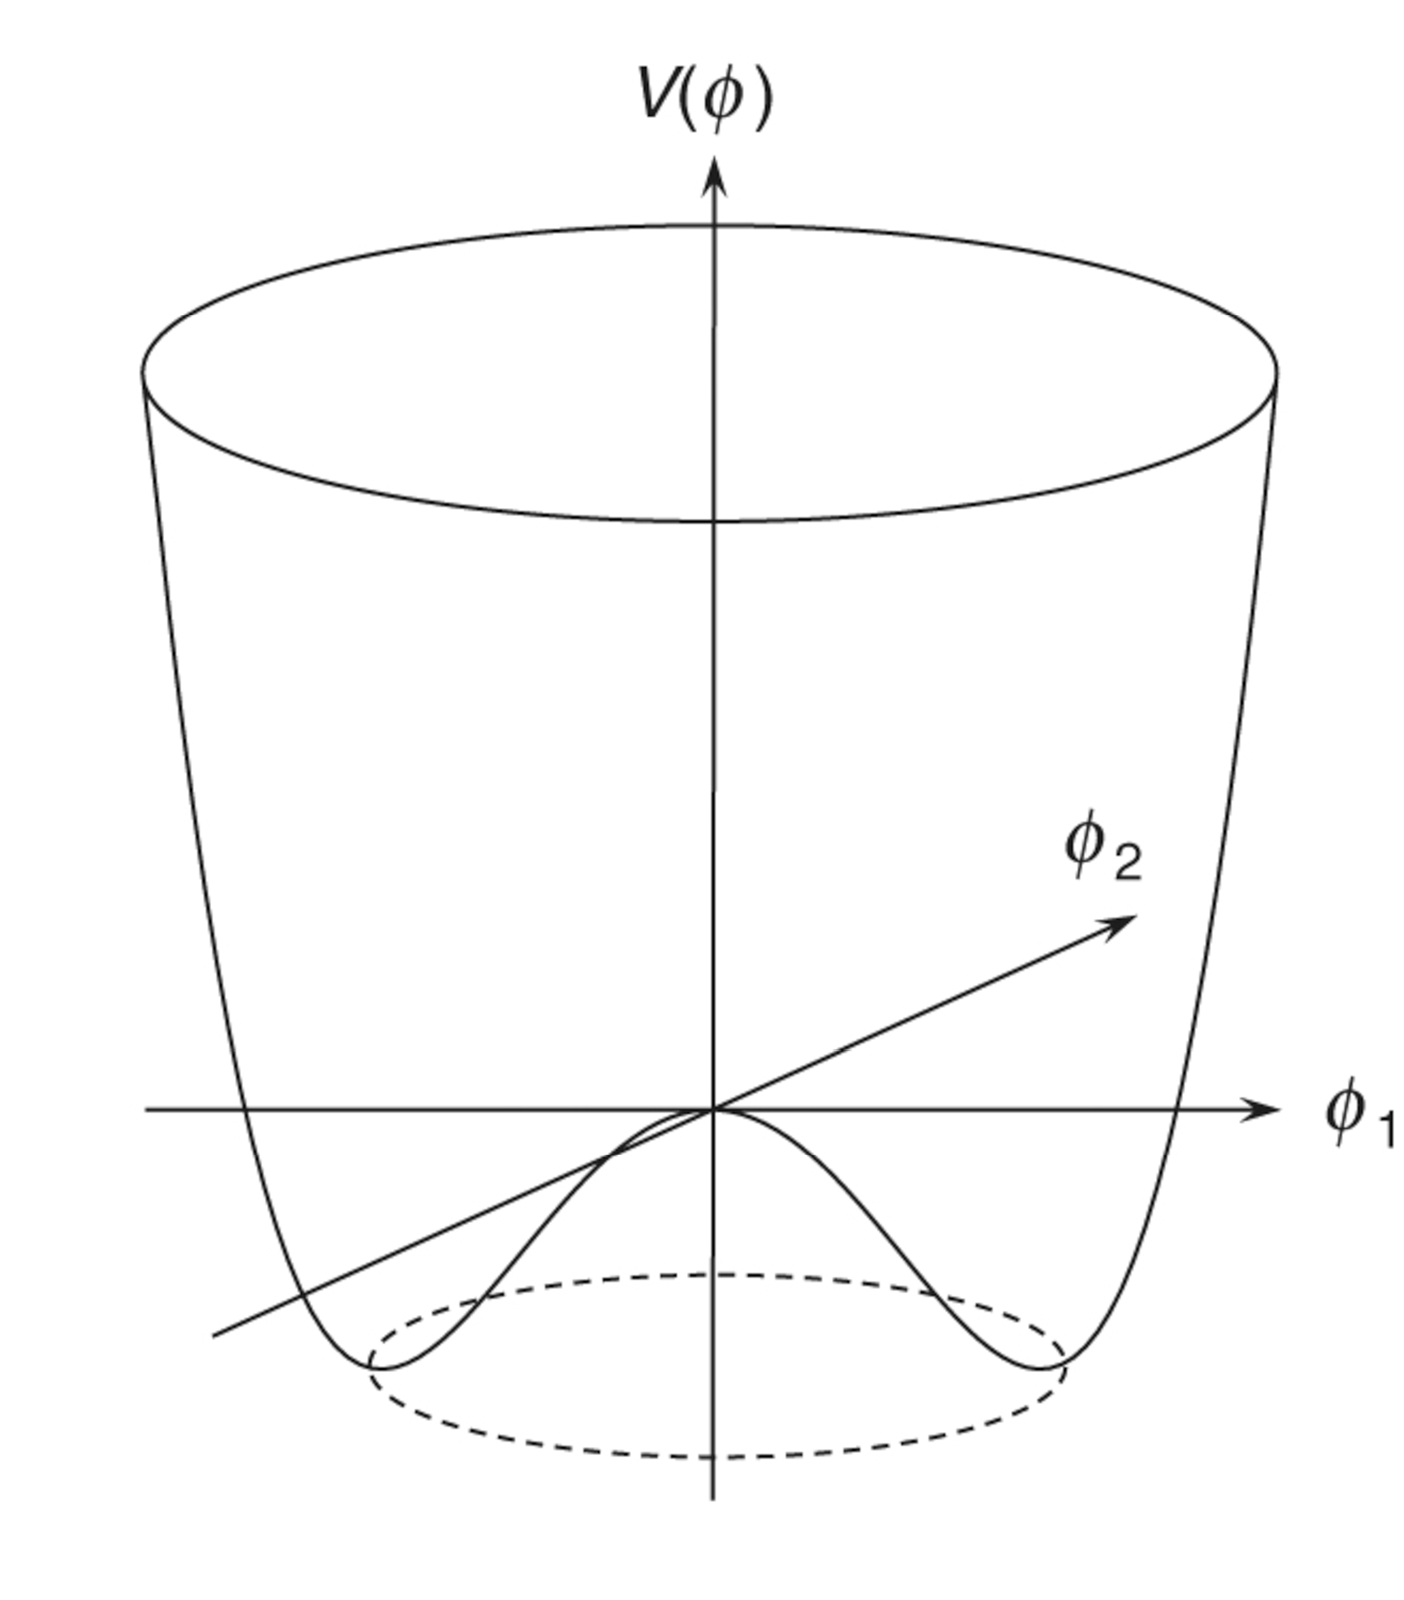
\includegraphics[width=0.45\textwidth]{Fig/HiggsPotential_MT1}\\
    \caption{The Higgs potential for $\mu^{2}<0$. \label{fig:HiggsPotential}}  
  \end{center}
\end{figure}
The potential is spherically symmetric, and thus the original Lagrangian is spherically symmetric.
For $\mu^{2}<0$, the potential has infinite degenerate minima
\begin{equation}
\label{eqn:Higgspotential}
\phi^{\dagger}\phi = \frac{1}{2}(\phi_{1}^{2}+\phi_{2}^{2}+\phi_{3}^{2}+\phi_{4}^{2})=\frac{v^{2}}{2}=-\frac{\mu^{2}}{2\lambda}.
\end{equation}
For the neutral photon to be massless after the symmetry breaking, the vacuum state is chosen to be
\begin{equation}
\label{eqn:Vacuum_Higgs}
\phi^{\text{vacuum}}=\frac{1}{\sqrt{2}}\begin{pmatrix}
  0 \\
  v  
 \end{pmatrix}
 .
\end{equation}
The symmetry of the original Lagrangian is broken, given that a particular ground state is selected among the degenerate states.
A field $\eta$ is introduced when applying the perturbation around the vacuum state 
\begin{equation}
\label{eqn:phi_Higgs}
\phi^{\text{vacuum}}=\frac{1}{\sqrt{2}}\begin{pmatrix}
  \phi_{1}+i\phi_{2} \\
  v + \eta + i\phi_{4} 
 \end{pmatrix}
 .
\end{equation}
By substituting Eq.~\ref{eqn:phi_Higgs} into the Lagrangian, however, will produce massless Goldstone bosons and terms associated with the couplings between the massive gauge fields and the Goldstone fields. An important fact is that every choice of the gauge transformation, as long as it follows correct form, will not break the symmetry of the Lagrangian. Therefore, a clever way to eliminate the Goldstone fields from the Lagrangian is to choose a gauge transformation called \emph{Unitary gauge}, and after which the complex scalar fields will be entirely real. The Higgs doublet after the Unitary gauge is written as
\begin{equation}
\label{eqn:phi_Higgs_UniGauge}
\phi^{\text{vacuum}}=\frac{1}{\sqrt{2}}\begin{pmatrix}
  0 \\
  v + h 
 \end{pmatrix}
 ,
\end{equation}
where $\eta$ is replaced by $h$, which represents the physical field. After expanding all the terms of the Lagrangian, the masses of gauge bosons can be identified as the coefficients of the quadratic in the gauge fields.

In the Higgs doublet, the lower component is neutral ($Q=0$) and has $I_{W}^{(3)}=-\frac{1}{2}$, therefore the whole doublet has weak hypercharge $Y=1$. 
Expanding the term $(D_{\mu}\phi)^{\dagger}(D^{\mu}\phi)$
\begin{equation}
\label{eqn:DmuDmu}
\begin{split}
(D_{\mu}\phi)^{\dagger}(D^{\mu}\phi) = & \frac{1}{2}(\partial_{\mu}h)(\partial^{\mu}h)+\frac{1}{8}g_{W}^{2}\big(W_{\mu}^{(1)}+iW_{\mu}^{(2)}\big)\big(W^{(1)\mu}-iW^{(2)}\mu\big)(v+h)^{2} \\	
& + \frac{1}{8}\big(g_{W}W_{\mu}^{(3)}-g^{\prime}B_{\mu}\big)\big(g_{W}W^{(3)\mu}-g^{\prime}B^{\mu}\big)(v+h)^{2}
\end{split}
.
\end{equation}
one can identify the quadratic terms as 
\begin{equation}
\label{eqn:quadterm}
\frac{1}{8}v^{2}g_{W}^{2}\bigg(W_{\mu}^{(1)}W^{(1)\mu}+W_{\mu}^{(2)}W^{(2)\mu}\bigg)+\frac{1}{8}v^{2}\bigg(g_{W}W_{\mu}^{(3)}-g^{\prime}B_{\mu}\bigg)\bigg(g_{W}W^{(3)\mu}-g^{\prime}B^{\mu}\bigg)
\end{equation}
Identify the mass of the $\PW$ boson by comparing
\begin{equation}
\frac{1}{2}m_{\PW}^{2}W_{\mu}^{(1)}W^{(1)\mu}=\frac{1}{8}v^{2}g_{W}^{2}W_{\mu}^{(1)}W^{(1)\mu},
\end{equation}
therefore
\begin{equation}
\label{eqn:WbosonMass}
m_{\PW}=\frac{1}{2}g_{W}v.
\end{equation}
The mass the physical $\PW$ boson is determined by the coupling constant of the $SU(2)_{L}$ gauge interaction $g_{W}$ and the vacuum expectation value of the Higgs field $v$.

The second term in Eq.~\ref{eqn:quadterm} is associated with the neutral $W^{(3)}$ and $B$ fields, and can be written as
\begin{equation}
\label{eqn:quadterm_neutral}
\begin{split}
\frac{1}{8}v^{2}\bigg(g_{W}W_{\mu}^{(3)}-g^{\prime}B_{\mu}\bigg)&\bigg(g_{W}W^{(3)\mu}-g^{\prime}B^{\mu}\bigg) = \\
& \frac{1}{8}v^{2}\begin{pmatrix}
  W_{\mu}^{(3)} & B_{\mu}
 \end{pmatrix}
 \begin{pmatrix}
  g_{W}^{2} & -g_{W}g^{\prime} \\
  -g_{W}g^{\prime} & g^{\prime 2}
 \end{pmatrix}
 \begin{pmatrix}
  W^{(3)\mu} \\
  B^{\mu}
 \end{pmatrix}
\end{split}
\end{equation}
The matrix (referred to as mass matrix) appearing in the equation is non-diagonal, showing that the off-diagonal elements couple the $W^{(3)}$ and $B$ fields and allow them to mix.
The physical boson fields (termed as $Z_{\mu}$ and $A_{\mu}$) correspond to the eigenstates of the mass matrix, which can be obtained by solving the characteristic equation 
\begin{equation}
\text{det}(\boldsymbol{M}-\lambda I) = (g_{W}^{2}-\lambda)(g^{\prime 2}-\lambda)-g_{W}^{2}g^{\prime 2} = 0.
\end{equation}
As a result, the eigenvalues $\lambda = 0\ \text{or}\ g_{W}^{2}+g^{\prime 2}$ with the eigenstates
\begin{equation}
\label{eqn:physicalfield_AZ}
\begin{split}
& A_{\mu} = \frac{g^{\prime}W_{\mu}^{(3)}+g_{W}B_{\mu}}{\sqrt{g_{W}^{2}+g^{\prime 2}}} ,\ \ m_{A}=0\ (\text{photon}) \\
& Z_{\mu} = \frac{g_{W}W_{\mu}^{(3)}-g^{\prime}B_{\mu}}{\sqrt{g_{W}^{2}+g^{\prime 2}}} ,\ \ m_{\cPZ}=\frac{1}{2}v\sqrt{g_{W}^{2}+g^{\prime 2}}\ (\cPZ\ \text{boson})
\end{split}
.
\end{equation}
Now, by defining the ratio of the coupling as
\begin{equation}
\label{eqn:tanthetaW}
\frac{g^{\prime}}{g_{W}}=\tan\theta	_{W},
\end{equation}
Eq.~\ref{eqn:physicalfield_AZ} can be expressed as
\begin{equation*}
\begin{split}
& A_{\mu}=+B_{\mu}\cos\theta_{W} + W_{\mu}^{(3)}\sin\theta_{W} \\
& Z_{\mu}=-B_{\mu}\sin\theta_{W} + W_{\mu}^{(3)}\cos\theta_{W}.
\end{split}
\end{equation*}
Eq.~\ref{eqn:Afield} and \ref{eqn:Zfield} are retained.
With Eq.~\ref{eqn:tanthetaW}, the mass of the physical $\cPZ$ boson is
\begin{equation}
m_{\cPZ}=\frac{1}{2}\frac{g_{W}}{\cos\theta_{W}}v.
\end{equation}
Combining with the $\PW$ boson mass from Eq.~\ref{eqn:WbosonMass}, one would obtain
\begin{equation}
\frac{m_{\PW}}{m_{\cPZ}}=\tan\theta_{W}.
\end{equation}
The mass of the Higgs boson $m_{\PH}$ can be identified as the quadratic term in the Higgs boson field which is generated by the potential $V(\phi)$ in the Lagrangian,
\begin{equation}
m_{H}^{2}=2\lambda v^{2}.
\end{equation}

In Eq.~\ref{eqn:DmuDmu}, the gauge boson fields appears in the form of $VV(v+h)^{2}$, where $V$ stands for gauge fields. 
The $VVv^{2}$ terms relate to the mass of the gauge bosons, and the $VVvh$ and $VVhh$ terms represent the triple and quartic couplings between the Higgs bosons and the gauge bosons.
From the weak theory, the physical $\PW$ bosons are constructed as linear combination of the $W^{(1)}$ and $W^{(2)}$, as shown in Eq.~\ref{eqn:Wboson}. Hence, the second term in Eq.~\ref{eqn:DmuDmu} associated with the $W^{(1)}$ and $W^{(2)}$ can be rewritten as 
\begin{equation}
\frac{1}{4}g_{W}^{2}W_{\mu}^{-}W^{+\mu}(v+h)^{2}=\frac{1}{4}g_{W}^{2}v^{2}W_{\mu}^{-}W^{+\mu}+\frac{1}{2}g_{W}^{2}vW_{\mu}^{-}W^{+\mu}h+\frac{1}{4}g_{W}^{2}W_{\mu}^{-}W^{+\mu}hh.
\end{equation}
The first terms gives the masses of $\PW$ boson as stated previous, the second term represents the triple $\PH\PWp\PWm$ coupling, and
the third term gives rise to the quartic $\PH\PH\PWp\PWm$ coupling.
The coupling strength of the $\PH\PWp\PWm$ vertex is 
\begin{equation}
g_{\PH\PW\PW}=\frac{1}{2}g_{W}^{2}v=g_{W}m_{\PW}.
\end{equation}
Similarly, the coupling $\PH\cPZ\cPZ$ can be derived $g_{\PH\cPZ\cPZ}=\frac{g_{W}}{\cos\theta_{W}}m_{\cPZ}\equiv g_{Z}m_{cPZ}$.
\emph{The couplings of the Higgs boson and the gauge bosons are proportional to the mass of the gauge bosons}. 
%Fig.~\ref{fig:HVVcouplings} shows the triple couplings of the Higgs boson to the $\PW$ and $\cPZ$ bosons.
%\begin{figure}[!ht]
%  \begin{center}  
%    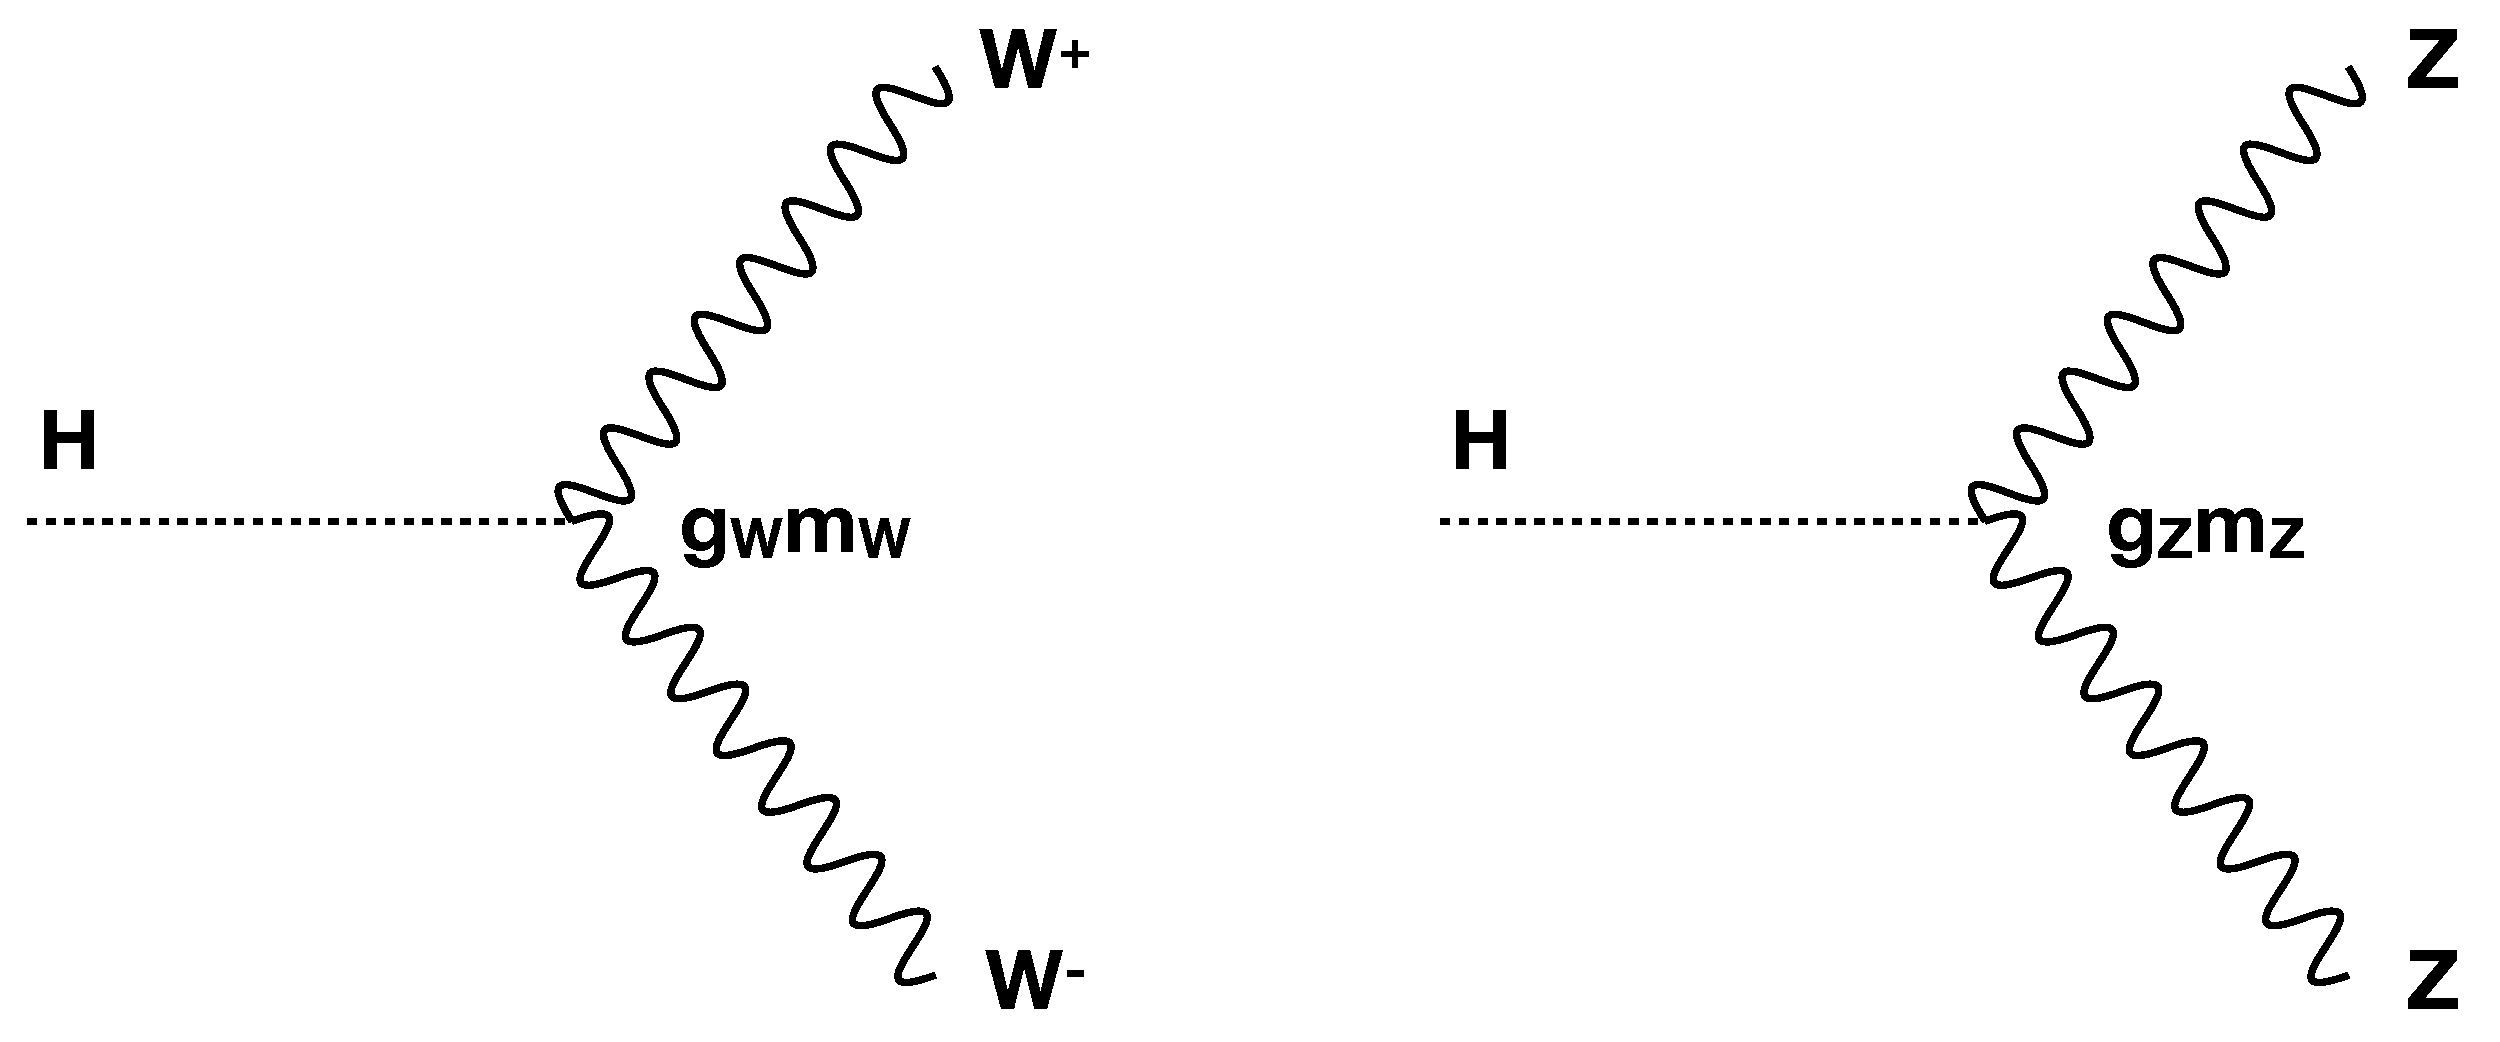
\includegraphics[width=0.7\textwidth]{Fig/HVVcouplings}
%    \caption{the triple couplings of the Higgs boson to the $\PW$ and $\cPZ$ bosons. \label{fig:HVVcouplings}}  
%  \end{center}
%\end{figure} 

As mentioned previously, the fermion mass term $-m\bar{\psi}\psi=-m\big(\bar{\psi}_{R}\psi_{L}+\bar{\psi}_{L}\psi_{R}\big)$ is not invariant under $\text{SU(2)}_{L}\times \text{U(1)}_{Y}$ transformation, since the RH and LH fermions transform differently
\begin{equation}
\begin{split}
& \text{LH doublet fermions}\ :\ \psi_{L}\ \to\ \psi_{L}^{\prime}=\psi_{L}\mathrm{e}^{ig_{W}\boldsymbol{T}\cdot\boldsymbol{W}+ig^{\prime}\frac{Y}{2}B} \\
& \text{RH singlet fermions}\ :\ \psi_{R}\ \to\ \psi_{R}^{\prime}=\psi_{R}\mathrm{e}^{ig^{\prime}\frac{Y}{2}B}
\end{split}
.
\end{equation}
The solution is to construct a \emph{singlet} under $\text{SU(2)}_{L}\times \text{U(1)}_{Y}$ in the Lagrangian.
Consider an infinitesimal SU(2) local transformaion on the SU(2) doublet $\phi$ of the Higgs fields,
\begin{equation}
\phi\to\phi^{\prime}=(I+ig_{W}\boldsymbol{\epsilon}(x)\cdot\boldsymbol{T})\phi,
\end{equation} 
where $\boldsymbol{T}$ are generators of the SU(2) group. 
The LH doublets $L$ undergoes the same transformation
\begin{equation}
\begin{split}
& L\to L^{\prime}=(I+ig_{W}\boldsymbol{\epsilon}(x)\cdot\boldsymbol{T})L \\
& \bar{L}=L^{\dagger}\gamma^{0}\to \bar{L}^{\prime} = \bar{L}(I-ig_{W}\boldsymbol{\epsilon}(x)\cdot\boldsymbol{T})
\end{split}
\end{equation}
It is clear that a term of $\bar{L}\phi$ is invariant under the $\text{SU(2)}_{L}$ transformation, or in other word, a singlet under $\text{SU(2)}_{L}\times \text{U(1)}_{Y}$. The effects of the transformation on the $\phi$ and $\bar{L}$ compensate to each other.
Combining the $\bar{L}\phi$ with RH singlet $R$ also results in a singlet under $\text{SU(2)}_{L}\times \text{U(1)}_{Y}$ (The conjugate of the combination is also a singlet).
Conseqently, a term in the Lagrangian of the form $-y_{f}(\bar{L}\phi R+ \bar{R}\phi^{\dagger}L)$ possesses the $\text{SU(2)}_{L}\times \text{U(1)}_{Y}$ gauge symmetry.
The Lagrangian, after spontaneous symmetry breaking and in the unitary gauge, is now 
\begin{equation}
\label{eqn:Lagrangian_fermionmass}
\mathcal{L}_{\text{fermion mass}} = -\frac{y_{f}}{\sqrt{2}}v(\bar{\ell}f_{R}+\bar{f}_{R}\ell)-\frac{y_{f}}{\sqrt{2}}(\bar{\ell}f_{R}+\bar{f}_{R}\ell).
\end{equation}
where $y_{f}$ is a constant known as \emph{Yukawa coupling}.
The first term corresponds to the fermion masses, $m_{\ell}=\frac{y_{f}v}{\sqrt{2}}$, representing the coupling of the fermions to the Higgs field through the non-zero vacuum expectation value. The second term corresponds to the interaction between the fermions and the physical Higgs boson.

The non-zero vacuum expectation value appears only in the lower component of the Higgs doublet, thus only fermions in the lower component of the SU(2) doublet (charged fermions and down-type quarks) can acquire masses, which is obviously not the case.
The way to give masses to up-type quarks is to construct the conjugate doublet of the Higgs field $\phi_{c}$ which transforms in the same way as the doublet $\phi$
\begin{equation}
\phi_{c}=-i\sigma_{2}\phi^{\ast}=\begin{pmatrix}
  -\phi^{0\ast} \\ 
  \phi^{-}
 \end{pmatrix} 
 = 
 \begin{pmatrix}
  -\phi_{3}+i\phi_{4} \\ 
  \phi_{1}-i\phi_{2}
  \end{pmatrix} 
\end{equation}
The Lagrangian of the up-type quark masses is the same as Eq.~\ref{eqn:Lagrangian_fermionmass} except $\phi$ now is replaced by $\phi_{c}$. 
Consequently, the Lagrangian, after the symmetry breaking, is
\begin{equation}
\label{eqn:Lagrangian_uptypemass}
\mathcal{L}_{\text{up-type quark masses}} = -\frac{y_{f,\ \text{up}}}{\sqrt{2}}v(\bar{u}u_{R}+\bar{u}_{R}u)-\frac{y_{f,\ \text{up}}}{\sqrt{2}}(\bar{u}u_{R}+\bar{u}_{R}u).
\end{equation}
where the up-type quark masses can be identified as $m_{\text{up}}=\frac{y_{f,\ \text{up}}v}{\sqrt{2}}$.
The Yukawa coupling of the fermions to the Higgs field is jointly written as
\begin{equation}
y_{f}=\frac{\sqrt{2}m_{f}}{v},
\end{equation}
and its value is determined to be consistent with the observed fermion masses.

The neutrino masses are yet another story. The possible mechanism to account for the neutrino masses was first introduced in Ref.~\cite{GellMann:1980vs,PhysRevLett.44.912}, and is now known as the seesaw mechanism. This mechanism will not be discusses in this thesis. 

A review of the Higgs boson production at the LHC will be introduced in the next sub-section. 

\subsection{The production of the Higgs boson and its decays}
The main production processes at the hadron collider are gluon-gluon fusion (ggF), vector boson fusion (VBF, or qqH), associated vector boson production (VH), and associated top quark pair production (ttH). The diagrams for these production modes are shown in Fig.~\ref{fig:higgsdiags} and the Higgs boson production cross-sections at the center-of-mass frame energy $\sqrt{s}=13\TeV$ are is shown in Fig.~\ref{fig:higgsXS}~\cite{LHCHXSWG}. 
The profound results of the deep inelastic scattering experiments showed that the momentum of the proton is not only carried by its three valence quarks, but also by the gluons that mediate the strong interaction between the quarks. In such a high energy collision at the LHC, the majority of energy is the carried by gluons, and hence the hard processes are dominantly produced by the gluon-gluon interactions.

\begin{figure}[!ht]
  \begin{center}  
    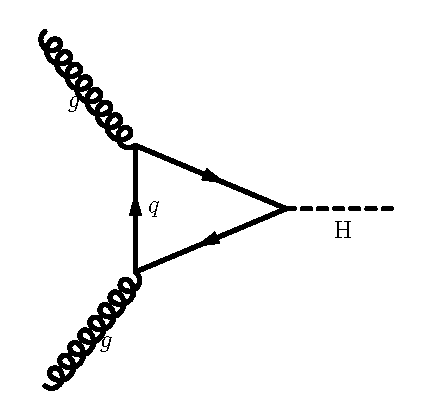
\includegraphics[width=0.3\textwidth]{Fig/Higgs_ggF}~
    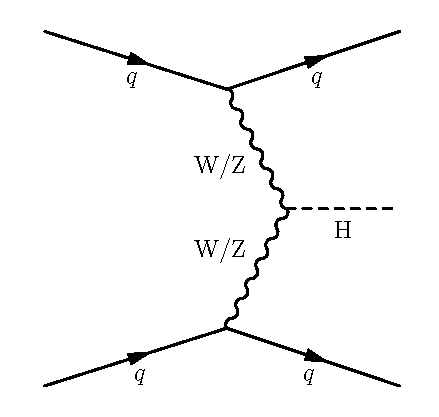
\includegraphics[width=0.3\textwidth]{Fig/Higgs_VBF}\\
    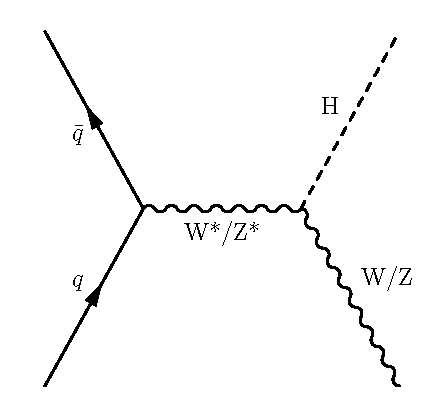
\includegraphics[width=0.3\textwidth]{Fig/Higgs_ZWH}~
    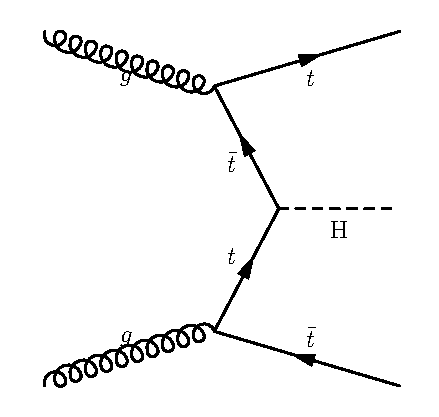
\includegraphics[width=0.3\textwidth]{Fig/Higgs_ttH}\\
    \caption{The diagrams for dominant production modes. (Top left) gluon-gluon fusion; (Top right) vector boson fusion; (Bottom left) associated vector boson production; (Bottom right) associated top quark pair production. \label{fig:higgsdiags}}  
  \end{center}
\end{figure} 

\begin{figure}[!ht]
  \begin{center}  
    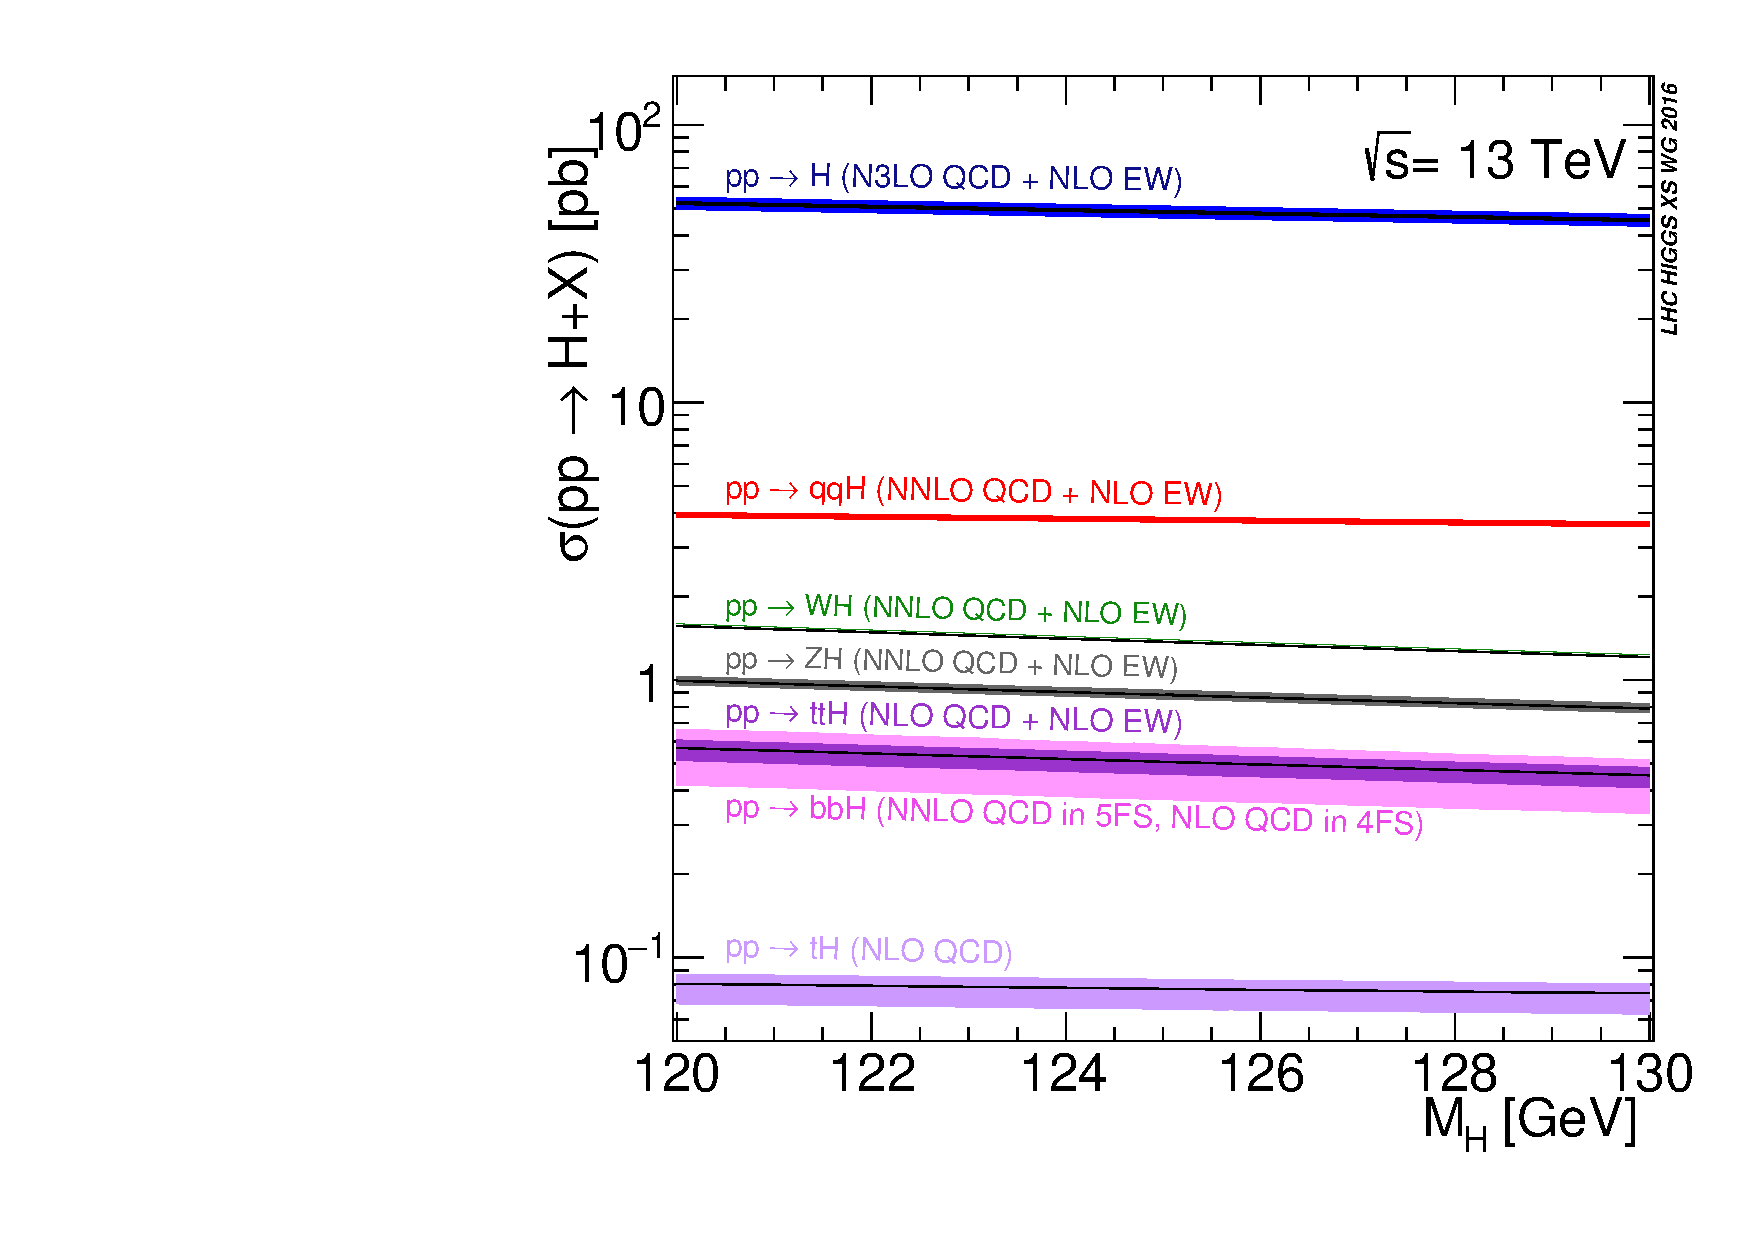
\includegraphics[width=0.6\textwidth]{Fig/plot_13tev_H_sqrt}\\
    \caption{The SM Higgs boson production cross sections at $\sqrt{s}=13\TeV$ as a function of the Higgs boson mass~\cite{LHCHXSWG}.\label{fig:higgsXS}}  
  \end{center}
\end{figure} 

Since the Higgs boson is the manifestation of the Higgs mechanism which gives fundamental particles masses, in principal it can decay into all particles, if it is kinematically allowed. The decay probability is interpreted as branching ratio. The branching ratio of the most important decay channels as function of the Higgs boson mass are shown in Fig.\ref{fig:higgsBR}. In the following paragraphs, I will discuss the main decay channels of the Higgs boson. 

\begin{figure}[!ht]
  \begin{center}  
    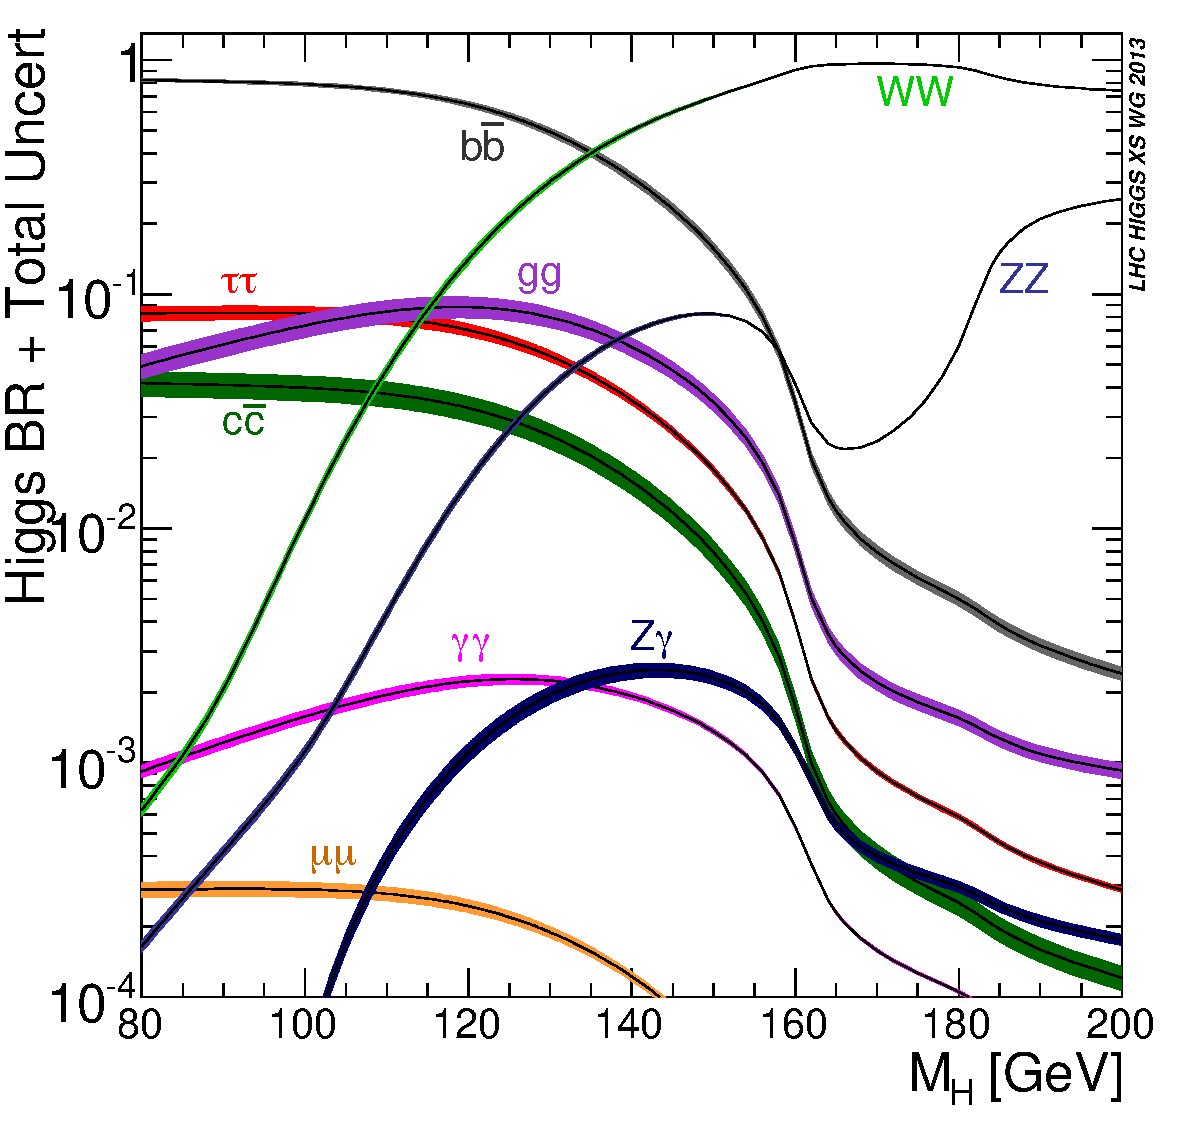
\includegraphics[width=0.6\textwidth]{Fig/Higgs_BR_LM}\\
    \caption{The SM Higgs boson decay branching ratios~\cite{LHCHXSWG}. \label{fig:higgsBR}}  
  \end{center}
\end{figure} 

The Higgs boson cannot decay into top quarks as the top quark is too heavy~\cite{LHCTOPWG}. The coupling between the Higgs boson and the top quark $y_{t}$ is then realized in terms of the ttH production and loops of virtual top quarks in the ggF production or in the decays to the massless particles, such as $\HGG$ and $\PH\to\Pg\Pg$. The combined measurement of the rate of Higgs boson production through gluon-gluon fusion and of the $\HGG$ decay with LHC Run1 data suggested that the Higgs boson coupling to top quarks is consistent with SM prediction within uncertainties~\cite{Khachatryan:2016vau}. A measurement of the production rate of the tree-level ttH process can provide further information as to whether there exists non-SM particles in the loops that introduce terms compensating for other deviations from the SM. The analysis is very difficualt, as the top-quark decays to a $\PW$ bosons and b-quark, and shortly afterwards the $\PW$ decays hadronically to two jets or leptonically to a lepton and a neutrino. Both the ATLAS and CMS Collaboration have recently observed this production channel, and established the confirmation of the tree-level coupling of the Higgs boson to top quarks with the combined analyses of datasets collected at $\sqrt{s}=7$, 8, and 13$\TeV$~\cite{Aaboud:2018urx,Sirunyan:2018hoz}. The best-fit signal strength $\hat{\mu}$ from the ATLAS measurement is $1.32^{+0.28}_{-0.26}(\text{Total})\ \pm 0.18(\text{Stat.})\ ^{+0.21}_{-0.19}(\text{Syst.})$, and from the CMS is $1.26^{+0.31}_{-0.26}(\text{Total})\ \pm 0.16(\text{Stat.})\ ^{+0.27}_{-0.22}(\text{Syst.})$. The ATLAS obtained a significance of 6.3 standard deviations ($\sigma$) relative to the background-only hypothesis, where the expected significance is $5.1\sigma$. The CMS also obtained the observed significance of $5.2\sigma$ with the expected significance is $4.2\sigma$. The Higgs-top coupling can also be probed in the search for the production of Higgs boson in association with a single top quark. The production cross-section of this process is not only sensitive to the absolute values of the modifiers of the Higgs-top coupling, $\kappa_{t}$, and the coupling of vector bosons to the Higgs boson, $\kappa_{V}$, but also to their relative signs with respect to those predicted in the SM. Hence, it provides additional information toward the nature of the Higgs boson. The CMS Collaboration performed this search with data collected in 2016~\cite{CMS-PAS-HIG-18-009}, and the results showed that the observed data favor positive sign of the coupling.

%\begin{figure}[!ht]
%  \begin{center}  
%    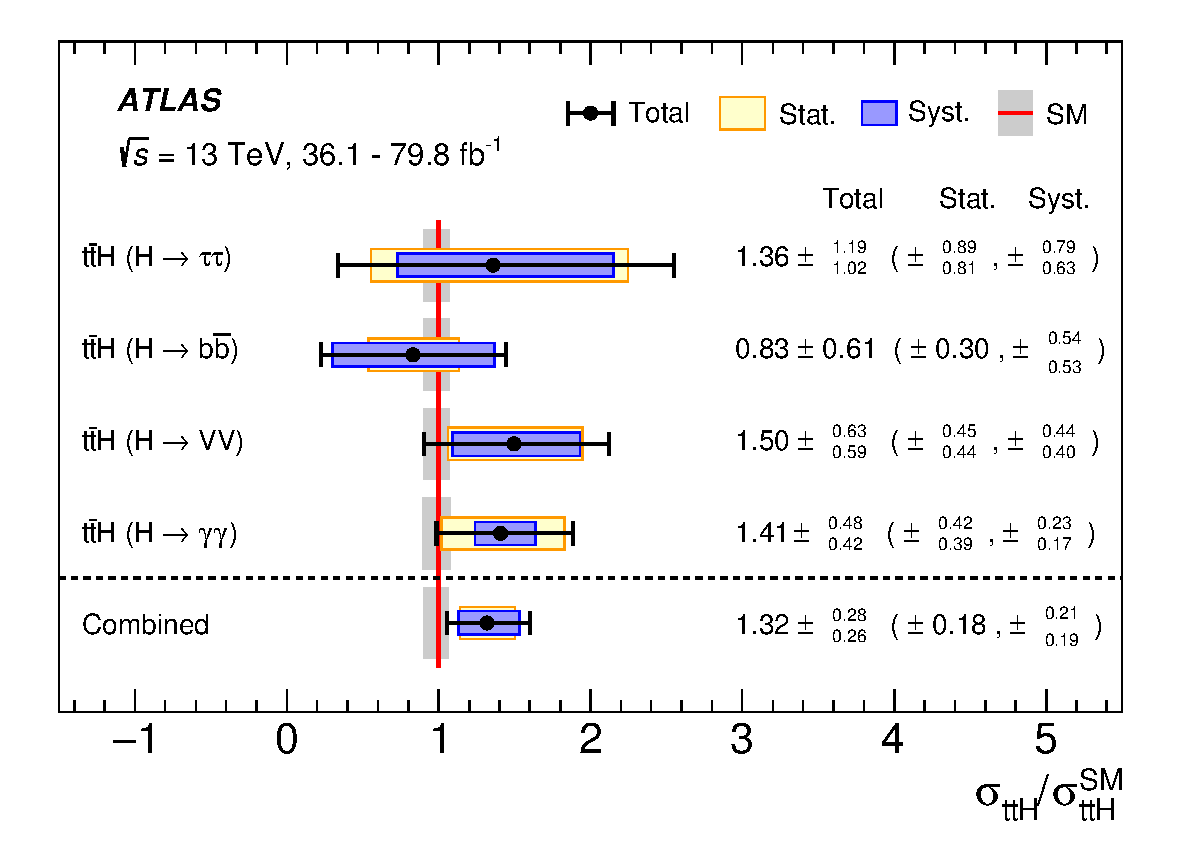
\includegraphics[width=0.56\textwidth]{Fig/figaux_02_ttHATLAS}~
%    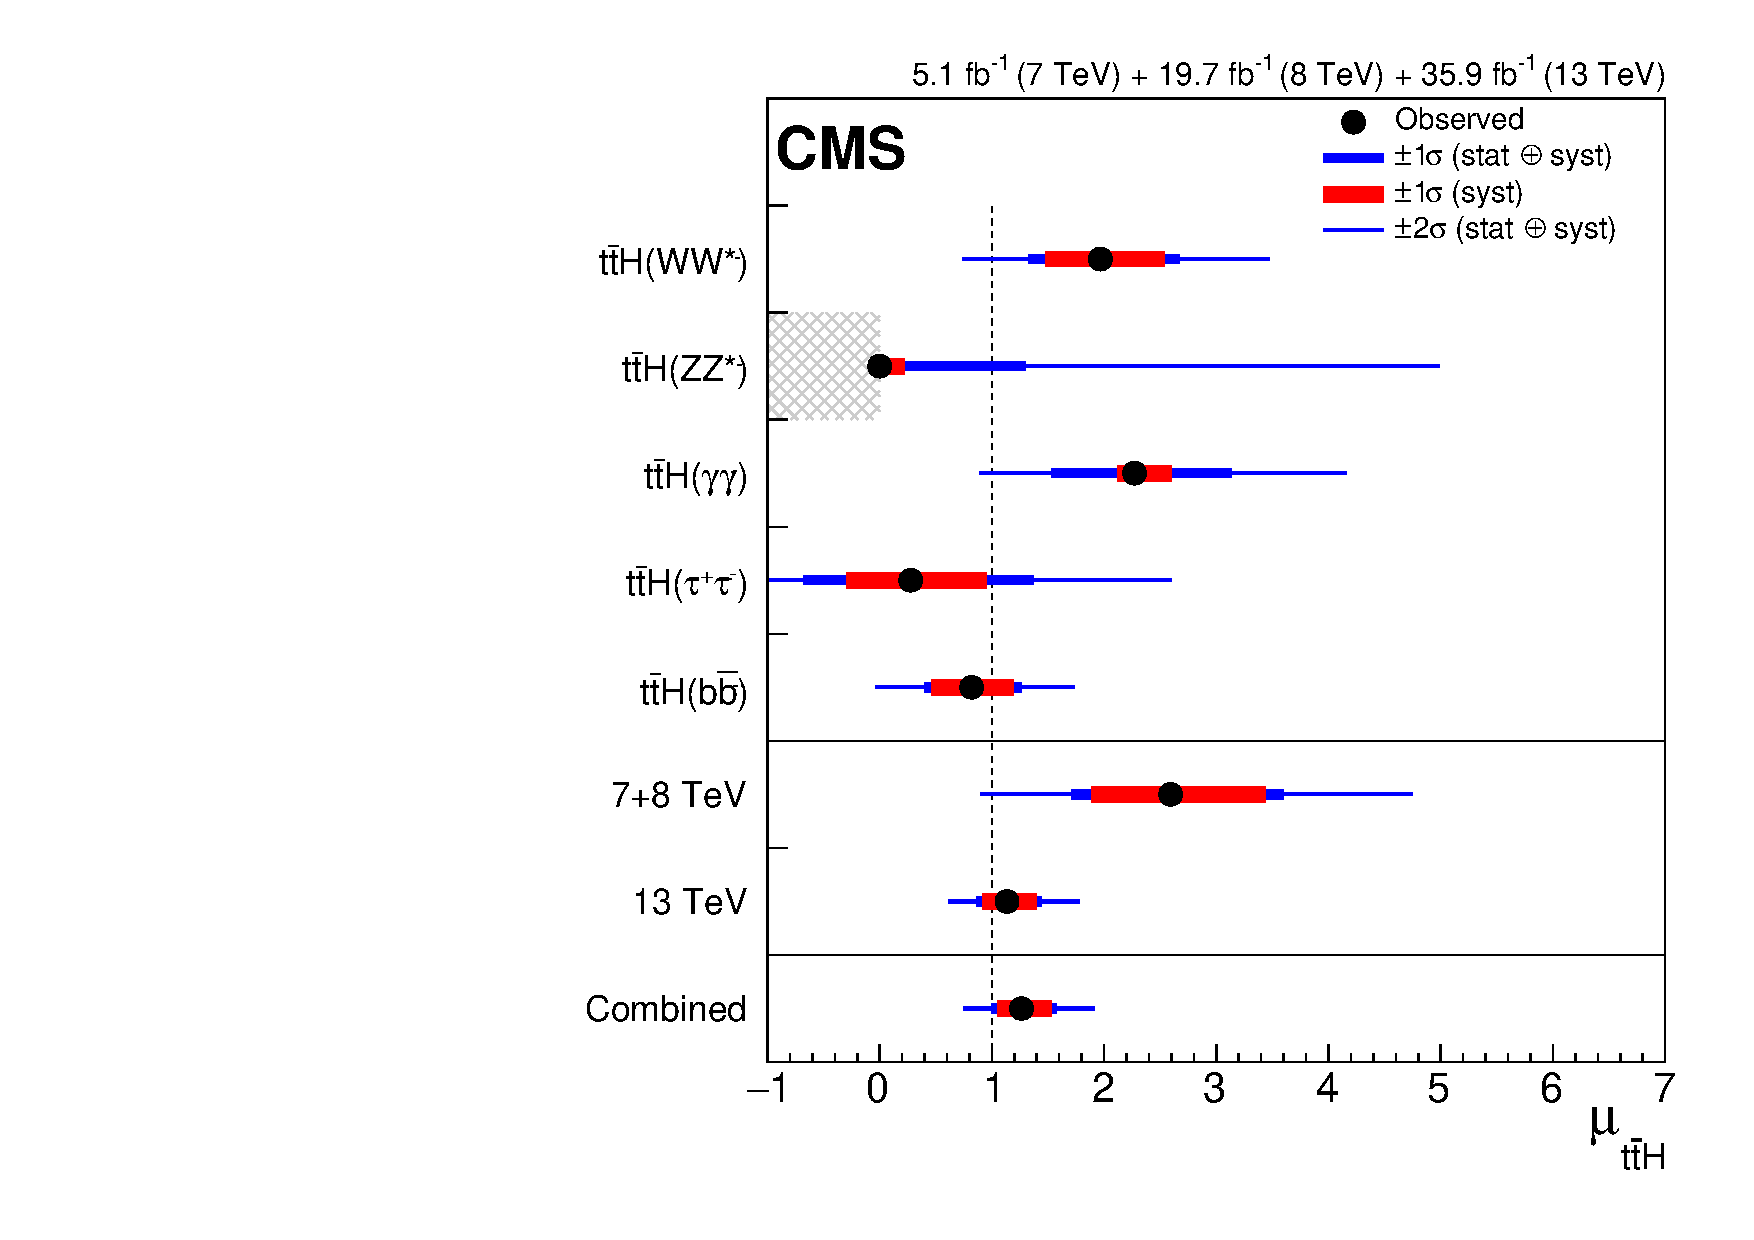
\includegraphics[width=0.44\textwidth]{Fig/CMS-HIG-17-035_Figure_001_ttHCMS}~
%    \caption{The best-fit signal strength $\hat{\mu}$ from both the ATLAS and CMS results. \label{fig:ttH_Observation}}  
%  \end{center}
%\end{figure} 
The largest branching ratio of the Higgs boson of mass $m_{\PH}=125\GeV$ is to bottom quarks, with $\mathcal{BR}(\PH\to\bbbar)\approx 58.2\%$. The measurement of the rate of the $\PH\to \bbbar$ decay offers a direct test to the magnitude of $\PH\cPqb\cPqb$ coupling, while the relative sign of the coupling can be determined by the decay process $\PH\to\Upsilon +\gamma$, where the $\Upsilon$ is the bound state of the b quarks~\cite{Bodwin:2013gca}. 
%In this channel, there are two hadronic jets in the final states, and hence the inclusive signal is overwhelmed by QCD multijets background $\Pp\Pp\to \bbbar+X$. 
In order to suppress the QCD backgrounds, the analysis is designed to search for the VH production where a W or Z boson decays leptonically, corresponding to five independent channels: $\cPZ(\ell\ell)\PH$, $\PW(\ell\nu)\PH$, and $\cPZ(\nu\nu)\PH$ where $\ell=\re, \mu$. A multivariate regression technique~\cite{Aaltonen:2011bp,Khachatryan:2015ota,Aad:2014xzb} is applied to calibrate the measured energy of the b-tagged jets to improve the dijet mass resolution, after which the mass resolution is approximately 10--15\%. The CMS Collaboration performs the search, and the combination with Run1 measurement results in an observed (expected) significance is 3.8 (3.8)$\sigma$. The corresponding signal strength $\hat{\mu}=1.06^{+0.31}_{-0.29}$~\cite{Sirunyan:2017elk}. The ATLAS Collaboration announces the first observation of this channel with data corresponding to an integrated luminosity of $79.8\fbinv$ collected in Run2 at $\sqrt{s}=13\TeV$~\cite{ATLAS-CONF-2018-036}. A combination with other production modes of the Higgs boson is performed for $\PH\to \bbbar$ decay mode, which yields an observed (expected) significance of 5.4 (5.5) $\sigma$. The signal strength $\hat{\mu}=1.01^{+0.20}_{-0.20}$.

The $\PH\to\TT$ decay mode has been considered as the only accessible leptonic decay mode that probes the coupling of the Higgs boson to the fermionic sector. It can also be used to constrain CP violation in the VBF production~\cite{Aad:2016nal} and provide sensitivity to CP violation in the Higgs boson coupling to leptons~\cite{Berge:2015nua}. This decay benefits from a favorable signal-to-background conditions than the $\PH\to \bbbar$ decay, however, slightly worse mass resolution of $\approx 10 - 20\%$, resulting from the inaccuracy of the momentum reconstruction of the $\PGt$ lepton. The $\PGt$ lepton can decay leptonically as $\PGt\to\nu_{\tau}\ell\bar{\nu}_{l}$ where $\ell=\re, \mu$, and hadronically to charged or neutral pions. The analyses from both the ATLAS and CMS utilizes the four most sensitive $\PGt\PGt$ final states: $\re\mu$, $\re\PGt_{h}$, $\mu\PGt_{h}$, and $\PGt_{h}\PGt_{h}$, where $\PGt_{h}$ denotes the hadronic decay. The ATLAS Collaboration reports the signal strength $\hat{\mu}=1.09^{+0.36}_{-0.30}$ with an observed (expected) significance of 6.4 (5.4) $\sigma$ with a combined analysis with $\sqrt{s}=$7, 8, and 13\TeV data~\cite{ATLAS-CONF-2018-021}. The CMS Collaboration also obtains the signal strength $\hat{\mu}=1.09^{+0.27}_{-0.26}$ with an observed (expected) significance of 5.9 (5.9) $\sigma$ in combination with Run1 data~\cite{Sirunyan:2017khh}.

Prior to the discovery of the Higgs boson, the decay mode $\PH\to\PW\PW$ was considered the most sensitive channel in the mass range around the $\PW\PW$ threshold of 160\GeV, and thus was important to the exclusion in such range. The $\PH\to\PW\PW^{*}\to\ell\nu\ell\nu$ analysis profits from the fact that it has large branching fraction and has a relatively low-background final state. As a result, this decay channel has very good sensitivity to most production processes, in particular ggF and VBF. However, the presence of neutrinos in the final state prevents the full reconstruction of the Higgs boson mass, and hence worse mass resolution of $\approx 20\%$. The different-flavor leptonic decay mode $\re\mu$ has the largest branching fraction, is the least affected by background processes, and therefore is the most sensitive channel of the analysis. The ATLAS Collaboration provides results of ggF and VBF production with 2016 data separately~\cite{ATLAS-CONF-2018-004}. For the ggF production the signal strength $\hat{\mu}=1.21^{+0.22}_{-0.21}$ with an observed (expected) significance of 6.3 (5.2) $\sigma$, while for the VBF the signal strength $\hat{\mu}=0.62^{+0.37}_{-0.36}$ with an observed (expected) significance of 1.9 (2.7) $\sigma$. The CMS Collaboration reports the signal strength $\hat{\mu}=1.28^{+0.18}_{-0.17}$ with an observed (expected) significance of 9.1 (7.1) $\sigma$, combining all considered channels~\cite{Sirunyan:2018egh}.

The $\PH\to\cPZ\cPZ^{*}\to 4\ell\ (\ell=\re\ \text{or}\ \mu)$ decay has low branching fraction, but fortunately has the lowest background contamination, resulting in very good sensitivity. It provides the direct probe in constraining the $\PH\cPZ\cPZ$ coupling. The precise reconstruction of the final state products allows the complete determination of the kinematics of the reconstructed Higgs boson with mass resolution of $\approx 1 - 2\%$, which makes it one of the most important channels to measure the properties of the Higgs boson. The ATLAS and CMS Collaborations have both performed analyses for this channel with the Run1 data to determine the mass and spin-parity of the boson~\cite{Chatrchyan:2013mxa,Chatrchyan:2012jja,Khachatryan:2014kca,Aad:2014eva,Aad:2015mxa}, its width~\cite{Khachatryan:2014iha,Khachatryan:2015mma,Aad:2015xua}, the fiducial cross sections [22, 23], and the tensor structure of its interaction with a pair of neutral gauge bosons~\cite{Khachatryan:2014kca,Aad:2015mxa,Khachatryan:2015mma}. These measurements provided results that are so far consistent with the SM predictions. The CMS Collaboration provides results, based on the combined data collected in 2016 and 2017, of the signal strength $\hat{\mu}=1.06^{+0.15}_{-0.13}$~\cite{CMS-PAS-HIG-18-001}. The ATLAS Collaboration reports the signal strength $\hat{\mu}=1.18^{+0.13}_{-0.13}$~\cite{ATLAS-CONF-2018-018}. A model-independent measurement of the Higgs boson width is performed by the CMS Collaboration with 2016 data using the $m_{4\ell}$ distribution in the range $105 < m_{4\ell} < 140\GeV$, and is able to constrain the width to be $\Gamma_{\PH}<1.10\ (1.60)\GeV$ at 95\% confidence level (CL) for observed (expected) value~\cite{Sirunyan:2017exp}.

Despite the small branching fraction predicted by the SM, the $\HGG$ decay provides a clean final state, two energetic photons, with an invariant mass peak that can be reconstructed with high precision with mass resolution of $\approx 1 - 2\%$. Consequently, this channel was one of the most important channels for the Higgs boson discovery and first measurements of its properties~\cite{Khachatryan:2014ira,Aad:2014eha}. Since the $\HGG$ decay proceeds mainly through $\PW$- and top-loop processes, interference effects make its branching fraction sensitive to the relative sign of the fermion and vector boson couplings. The differential cross sections enables us to test the perturbative QCD predictions for Higgs boson production, and can be used to probe the spin and CP properties of the Higgs boson. The CMS Collaboration provides the results using 2016 data of the signal strength $\hat{\mu}=1.18^{+0.17}_{-0.14}$~\cite{Sirunyan:2018ouh}, while the ATLAS Collaboration obtains $\hat{\mu}=0.99^{+0.14}_{-0.14}$. The interpretation of the coupling measurements from both collaborations shows that the observed data favors the positive sign of the coupling~\cite{Sirunyan:2018kta,Aaboud:2018xdt}. The ATLAS Collaboration also tries to investigate the strength and tensor structure of the Higgs boson interactions using an effective Lagrangian, which introduces additional CP-even and CP-odd interactions~\cite{Aaboud:2018xdt}, but no significant new physics contributions are observed.

The decay of $\PH\to\cPZ/\gamma^{*}+\gamma$ shares almost the same diagrams as that of the $\HGG$ decay, where in the former one a $\cPZ$ boson or a virtual photon $\gamma^{*}$ is radiated from the loop. Measurement of this rare decay can enhance the current understanding of the nature of the Higgs boson, and can also provide an alternative way to test if there is any beyond standard model (BSM) couplings induced in the loop diagrams. A brief summary of these extension of SM can be found in Ref.~\cite{Sirunyan:2018tbk,Aaboud:2017uhw}. If there exists BSM that is manifested through CP violation, one can also observe the anomaly though a measurement of the forward-backward asymmetry. The ATLAS Collaboration sets an observed (expected) exclusion upper limit on the production cross section times the branching ratio of the $\PH\to\cPZ\gamma$ decay of 6.6 (5.2) times the SM prediction at 95\% CL for a Higgs boson mass $m_{\PH}=125.09\GeV$, while the upper limits from the CMS Collaboration varies between 6.1 and 11.4 (3.9 and 9.1) times the SM value in the mass range of $120<m_{\PH}<130\GeV$~\cite{Sirunyan:2018tbk,Aaboud:2017uhw}. The CMS Collaboration also provides so far the most stringent limit on the $\PH\to\gamma^{*}\gamma$ decay, varying between 1.4 and 4.0 (2.1 and 2.3) times the SM prediction in the range of $120<m_{\PH}<130\GeV$~\cite{Sirunyan:2018tbk}.

The rare decay $\PH\to\mu\mu$ offers the best possibility to measure the Higgs coupling to second-generation fermions at the LHC. The expected branching fraction for a Higgs boson mass $m_{\PH}=125.09\GeV$ is $\mathcal{BR}(\PH\to\mu\mu)\approx 2.2\ten{-4}$~\cite{deFlorian:2016spz} which is roughly one order of magnitude smaller than the $\PH\to\cPZ/\gamma^{*}+\gamma$ decay, owing to the small Yukawa coupling of the muon to the Higgs field. The CMS Collaboration sets the observed (expected) upper limit on the signal strength of 2.92 (2.16) times the SM prediction, with combination of 7, 8, and 13\TeV data~\cite{Sirunyan:2018hbu}, while the ATLAS Collaboration reports an upper limit of 2.1 (2.0) times the SM values~\cite{ATLAS-CONF-2018-026}.

The other decay of the Higgs boson to second-generation fermions that was searched for is the $\PH\to\ccbar$ process. It is commonly considered impossible to discover this channel even in high luminosity run of the LHC (HL-LHC) due to the small branching fraction, large background in hadron collider, and jet flavor identification inefficiency~\cite{Perez:2015aoa,Perez:2015lra}. Nevertheless, direct search for the $\PH\to\ccbar$ decay is important in the long-term perspective, as the development of the charm-tagging technique and the direct constraint of the Higgs-charm coupling would be valuable inputs to the next generation of particle colliders. The ATLAS Collaboration presents the first search for this process with data collected in 2016, utilizing the $\cPZ\PH$ production with the subsequent decay of the Z boson to dilepton. The observed (expected) upper limit on the production cross-section $\sigma(\Pp\Pp\to\cPZ\PH)\times\mathcal{BR}(\PH\to\ccbar)$ is found to be $2.7\ (3.9^{+2.1}_{-1.1})\pb$ at the 95\% CL, corresponding to an observed (expected) upper limit on  the signal strength $\hat{\mu}<110\ (150^{+80}_{-40})$~\cite{Aaboud:2018fhh}.

\subsection{The measurement of the Higgs coupling}
The ATLAS and CMS Collaborations both reported the observation of a new boson with a mass of $m_{\PH}=125.09\pm 0.21(\text{stst.})\pm 0.11(\text{syst.})\GeV$~\cite{Aad:2015zhl} in 2012, and subsquent mesurements revealed its Higgs-boson-like properties~\cite{Chatrchyan:2012jja,Khachatryan:2014kca,Aad:2012tfa,Chatrchyan:2012xdj,Chatrchyan:2013lba,Aad:2015gba,Khachatryan:2014jba,Aad:2013xqa}. One of the important analyses, and most related to this thesis, is the measurement of the Higgs coupling.  A combined measurement were performed by ATLAS and CMS with data collected at 7 and 8\TeV~\cite{Khachatryan:2016vau}, and the CMS Collaboration provides the latest results with 13\TeV data~\cite{CMS-PAS-HIG-17-031}. The results from CMS with 13\TeV data will be shown in the following paragraphs.

The inputs of the analysis are the four main production processes introduced previously, decay channels to bosons $\PH\to\cPZ\cPZ,\ \PW\PW,\ \PGg\PGg$, and to fermions $\PH\to\PGt\PGt,\ \bbbar,\ \PGm\PGm$. In this work, a so-called $\kappa-$framework~\cite{Heinemeyer:2013tqa} is used\footnotemark. 
\footnotetext{It was referred to as Interim framework in the cited reference.}
Within the framework, there are assumptions made such that the production and decay of the Higgs boson can be factorized and parametrized as 
\begin{equation}
\sigma_{i}\cdot\mathcal{BR}^{f}=\frac{\sigma_{i}(\overrightarrow{\kappa})\cdot\Gamma^{f}(\overrightarrow{\kappa})}{\Gamma_{\PH}},
\end{equation}
where $\Gamma_{\PH}$ is the total width of the Higgs boson and $\Gamma^{f}$ is the partial width for Higgs boson decay to the final state $f$. Coupling modifiers, $\overrightarrow{\kappa}$, are introduced in order to test deviations in the couplings of the Higgs boson to other particles, and are defined as 
\begin{equation}
\kappa_{j}^{2}=\frac{\sigma_{j}}{\sigma_{j}^{\text{SM}}}\ \text{or}\ \kappa_{j}^{2}=\frac{\Gamma^{j}}{\Gamma^{j}_{\text{SM}}},
\end{equation}
where all $\kappa_{j}=1$ in the SM and $j$ denotes the tested production or decay mode.
Tree-level Higgs boson couplings, such as the $\PH-\cPZ,\ \PH-\PW,\ \PH-t,\ \PH-b,\ \PH-\PGt,\ \text{and}\ \PH-\PGm$, are introduced as individual coupling modifiers. For those processes that occur at leading-order (LO) involving box or triangular loop diagrams, the loops are resolved in terms of the corresponding coupling modifiers, weighted by their individual contribution. Interference effects between the different diagrams provide sensitivity to the relative signs of the Higgs boson couplings to different particles. The coupling modifiers $\kappa_{\cPqc}$ and $\kappa_{\PQs}$ are allowed to vary as function of other modifiers, provided that current LHC data are insensitive to these couplings. The constraint on $\kappa_{\cPqc}$ will be introduced separately later. Other coupling modifiers $\kappa_{\PQu}$, $\kappa_{\PQd}$, and $\kappa_{\re}$ are not included in combination given that their magnitudes are marginal. 

There are two parametrization schemes. One is defined such that two additional effective coupling modifiers, $\kappa_{\cPg}$ and $\kappa_{\PGg}$, which describe the loop processes for ggF production and $\HGG$ decay, are introduced to account for the situation that BSM particles may be present in these loops. The other one is to resolve the ggF and $\HGG$ processes as function of remaining coupling modifiers. 
Fig.~\ref{fig:kappaCMS2016_1} shows the summary plots for the $\kappa$-framework model with the resolved loop scheme and the assumption $\mathcal{BR}_{\text{BSM}}=0$. The points indicate the best fit values while the thick and thin horizontal bars show the $1\sigma$ and $2\sigma$ CL intervals, respectively. Without loss of generality, the value of $\kappa_{\PQt}$ is restricted to be positive. For this model, both positive and negative values of $\kappa_{\PW}$, $\kappa_{\cPZ}$, and $\kappa_{\PQb}$ are considered. The result shows that negative values of $\kappa_{\PW}$ are disfavored by more than $2\sigma$. The interference between diagrams of the $\cPZ\PH$ production leads to the break of the degeneracy between signs, and indicates that a positive value of $\kappa_{\cPZ}$ is favored. A negative value of $\kappa_{\PQb}$ is preferred in this model, however, the difference between the best-fit point and the minimum in the positive region is small. 
Fig.~\ref{fig:kappaCMS2016_2} shows the summary plots with effective couplings scheme. In the left figure the constraint $\mathcal{BR}_{\text{BSM}}=\mathcal{BR}_{\text{inv}}+\mathcal{BR}_{\text{undet}}=0$ is imposed, and both positive and negative values of $\kappa_{\PW}$ and $\kappa_{\cPZ}$ are considered. In the right figure a constraint $|\kappa_{V}| \leq 1$, where $\kappa_{V}$ denotes $\kappa_{\cPZ}$ or $\kappa_{\PW}$, is imposed (same sign of $\kappa_{\cPZ}$ and $\kappa_{\PW}$), while $\mathcal{BR}_{\text{inv}} > 0$ and $\mathcal{BR}_{\text{undet}} > 0$ are free parameters. The preferred sign of the $\kappa_{\PW}$, opposite to the first scheme, is negative. In Fig.~\ref{fig:kappaCMS2016_3}, left plot shows the scan of the test statistic as a function of $\mathcal{BR}_{\text{inv}}$, and the right plot shows the 68\% and 95\% CL contours for $\mathcal{BR}_{\text{inv}}$ vs. $\mathcal{BR}_{\text{undet}}$, indicating the 95\% CL upper limits of $\mathcal{BR}_{\text{inv}}<0.22$ and $\mathcal{BR}_{\text{undet}}<0.36$.

\begin{figure}[!ht]
\begin{center}
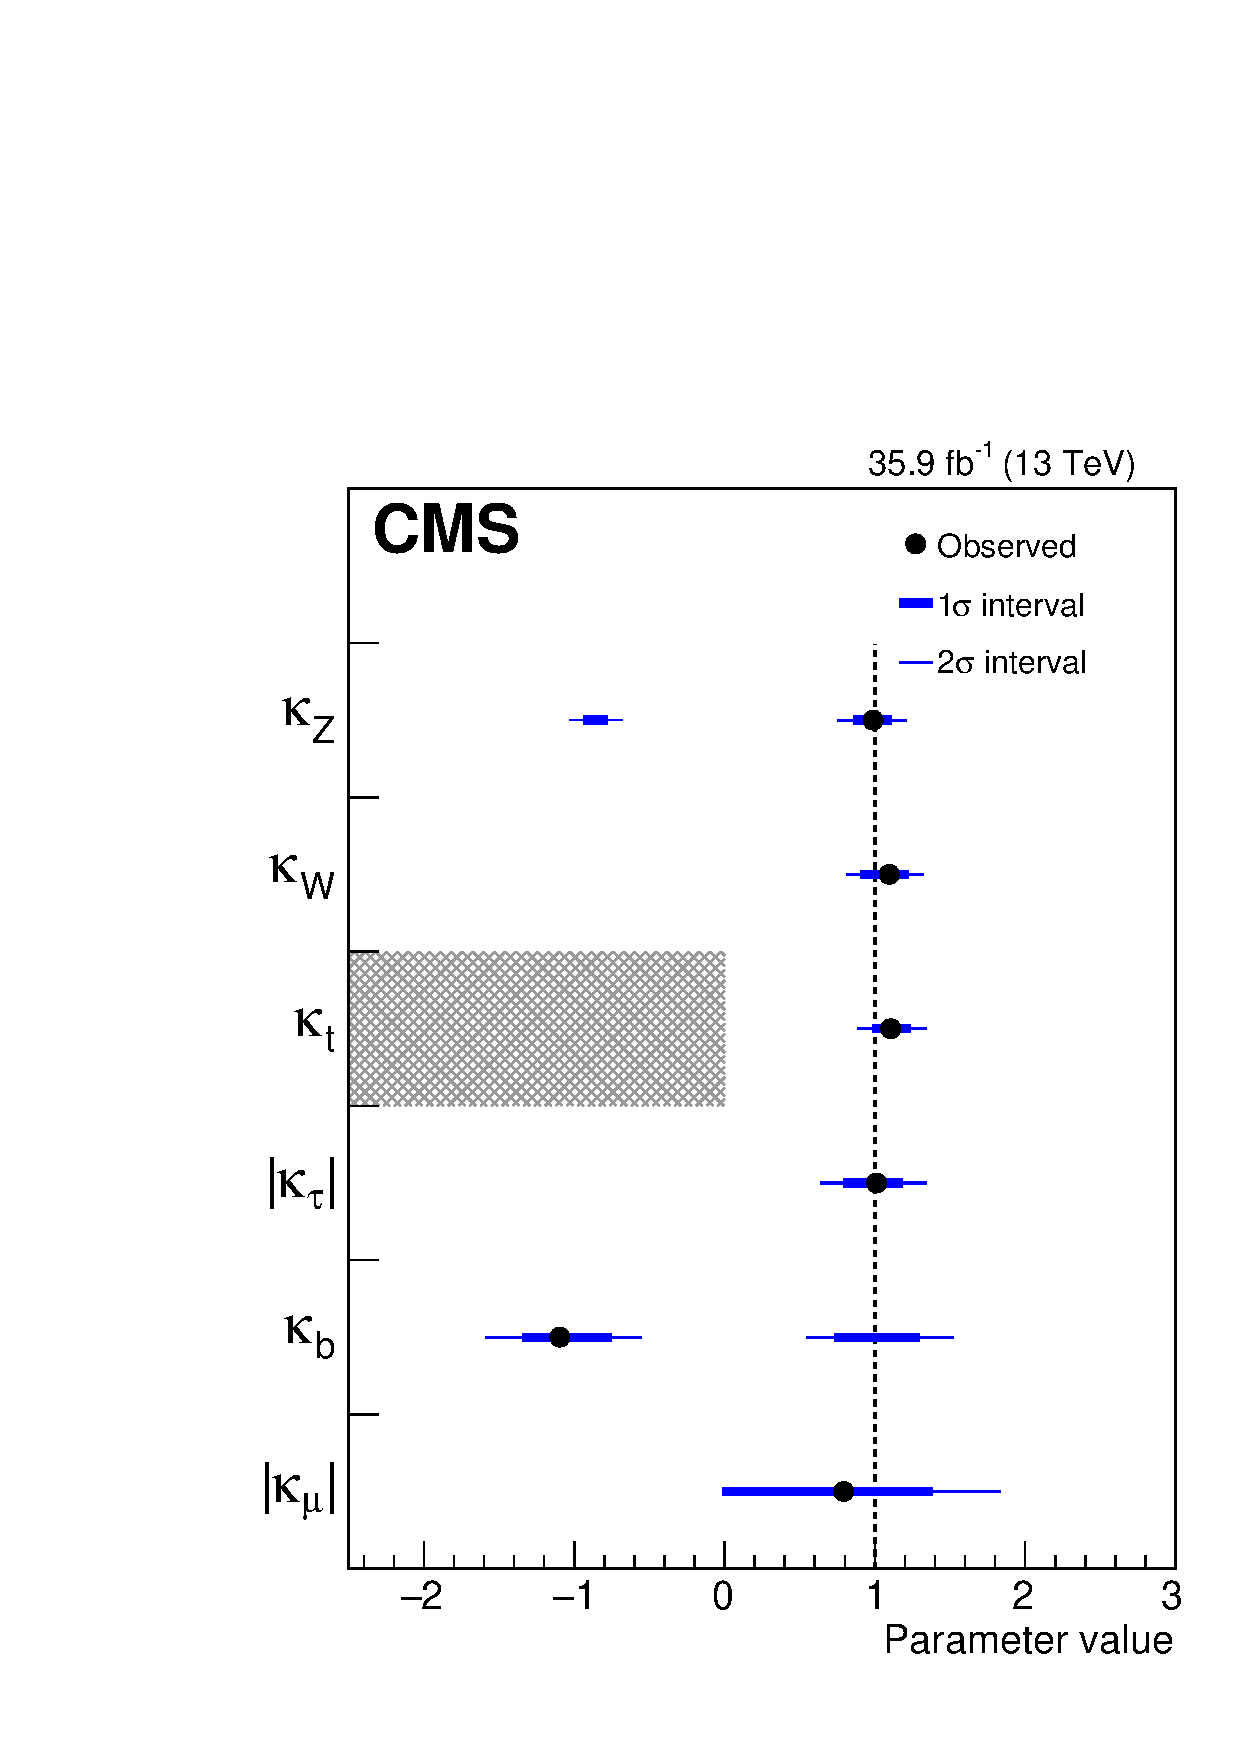
\includegraphics[width=0.5\textwidth]{Fig/HIG17031/plot_K1_mm_merged}\\
\caption{Summary for the $\kappa$-framework model with the resolved loop scheme~\cite{CMS-PAS-HIG-17-031}. \label{fig:kappaCMS2016_1}}
\end{center}
\end{figure}

\begin{figure}[!ht]
\begin{center}
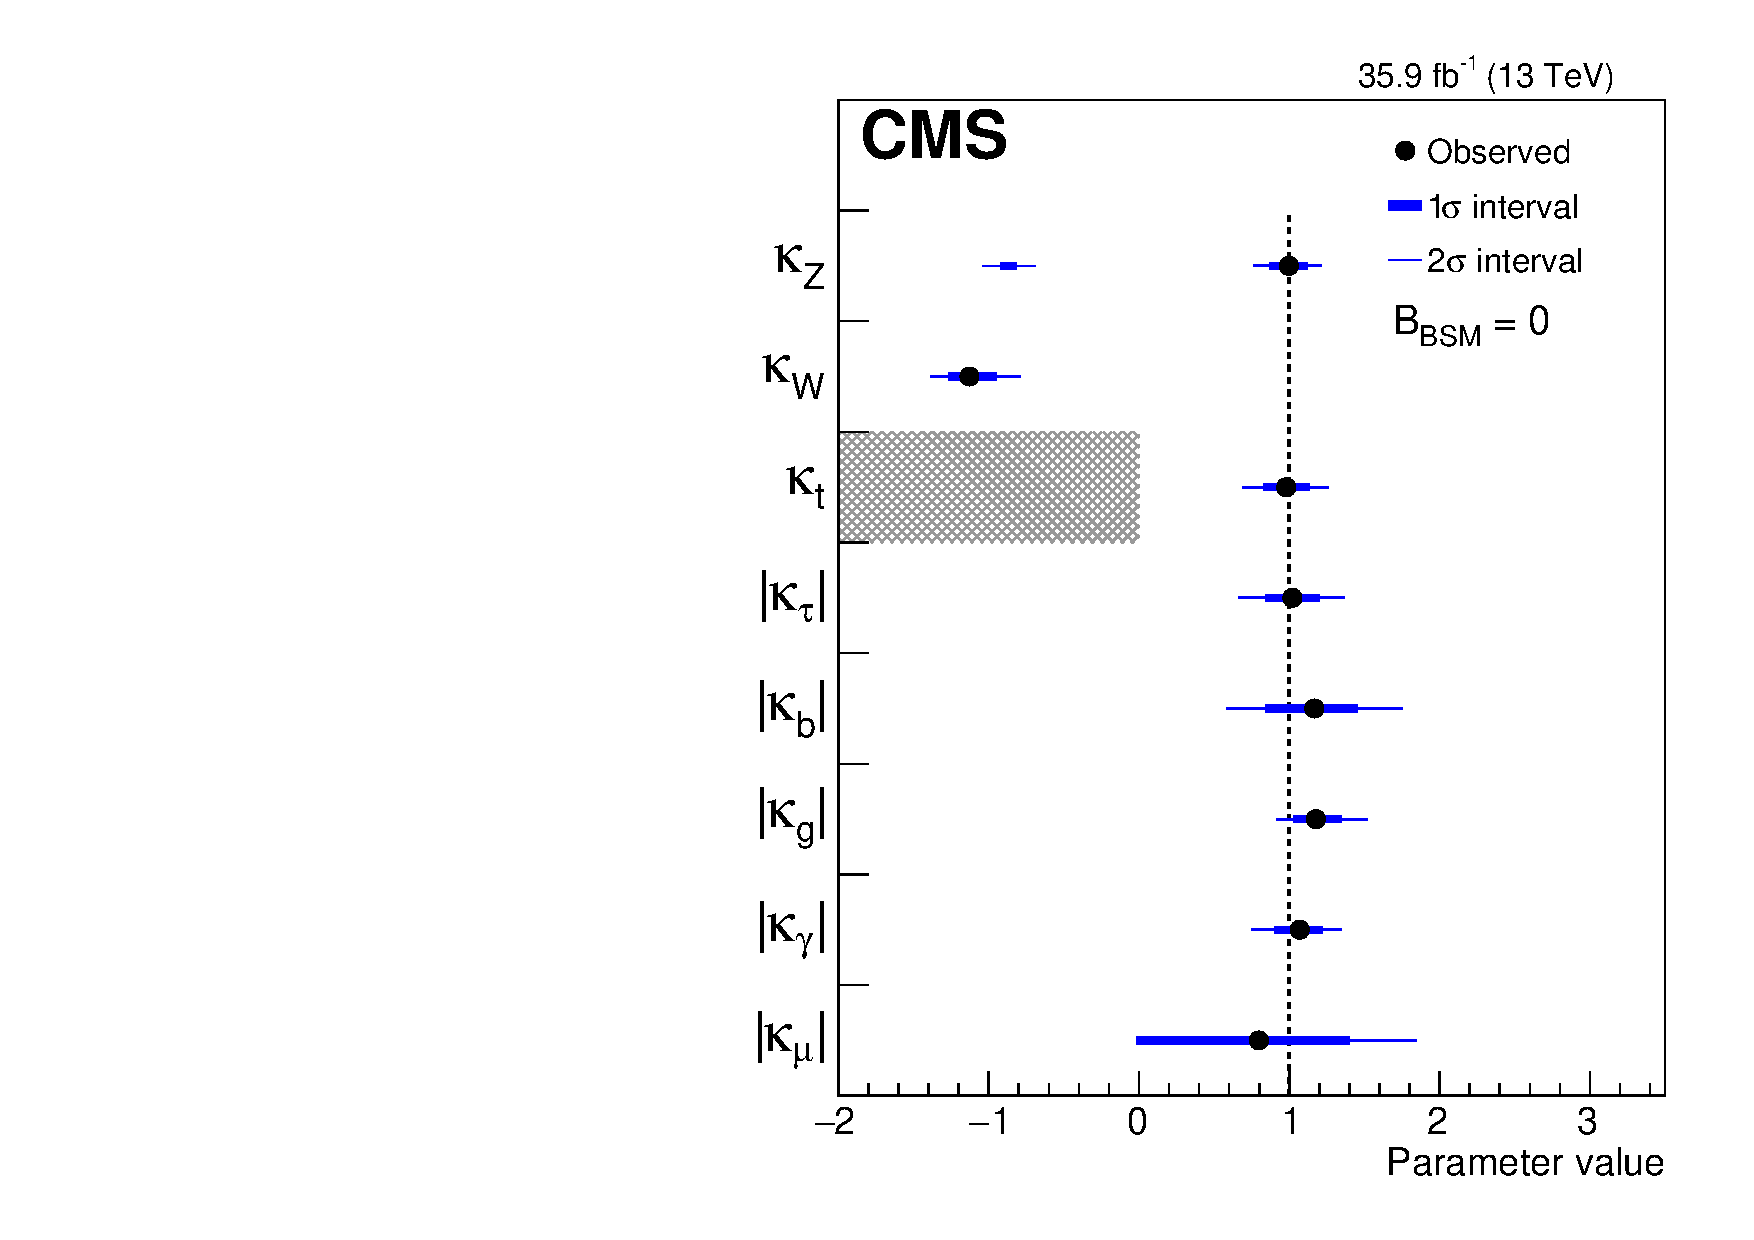
\includegraphics[width=0.56\textwidth]{Fig/HIG17031/plot_K2_merged}~
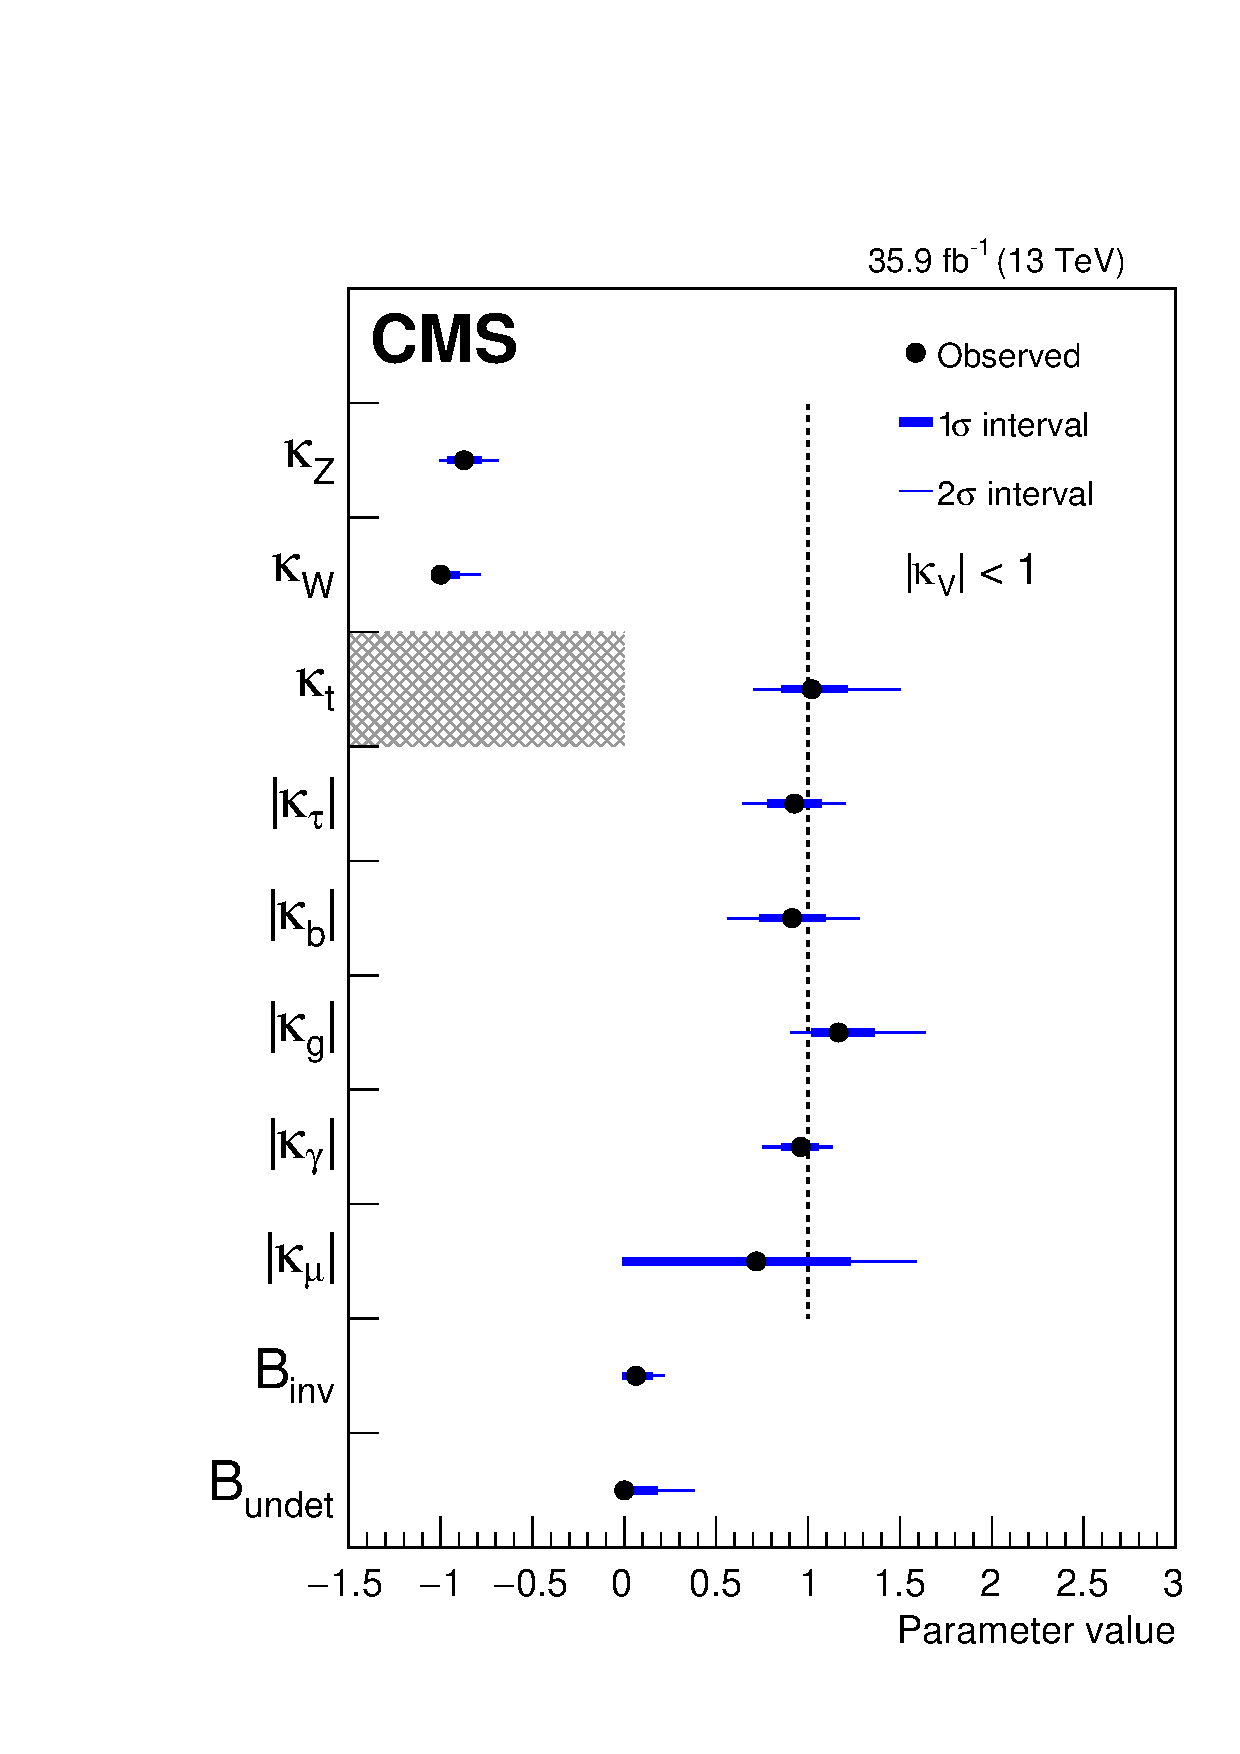
\includegraphics[width=0.44\textwidth]{Fig/HIG17031/plot_K2Undet_merged}\\
\caption{Summary for the $\kappa$-framework model with the effective couplings scheme~\cite{CMS-PAS-HIG-17-031}. \label{fig:kappaCMS2016_2}}
\end{center}
\end{figure}

\begin{figure}[!ht]
\begin{center}
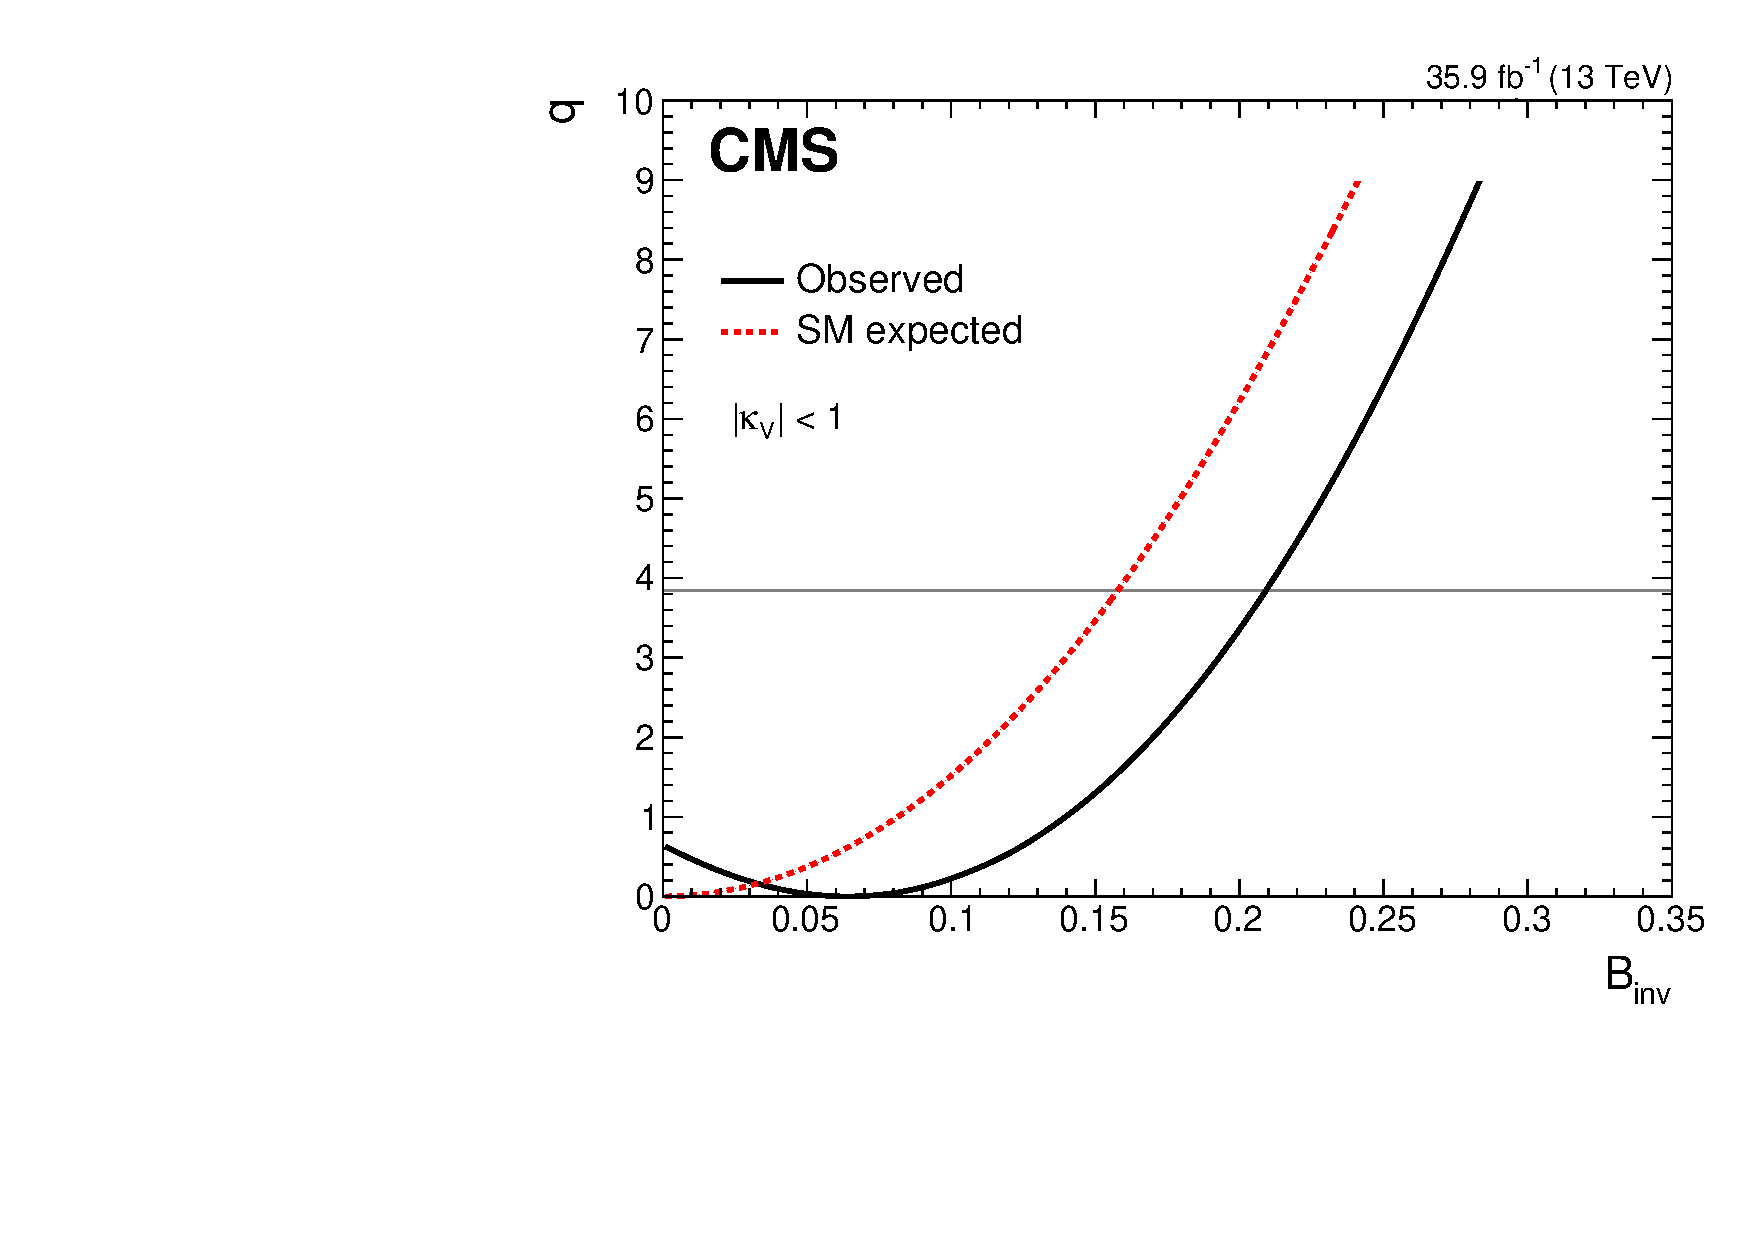
\includegraphics[width=0.535\textwidth]{Fig/HIG17031/scan_pub_observed_K2Undet_BRinv}~
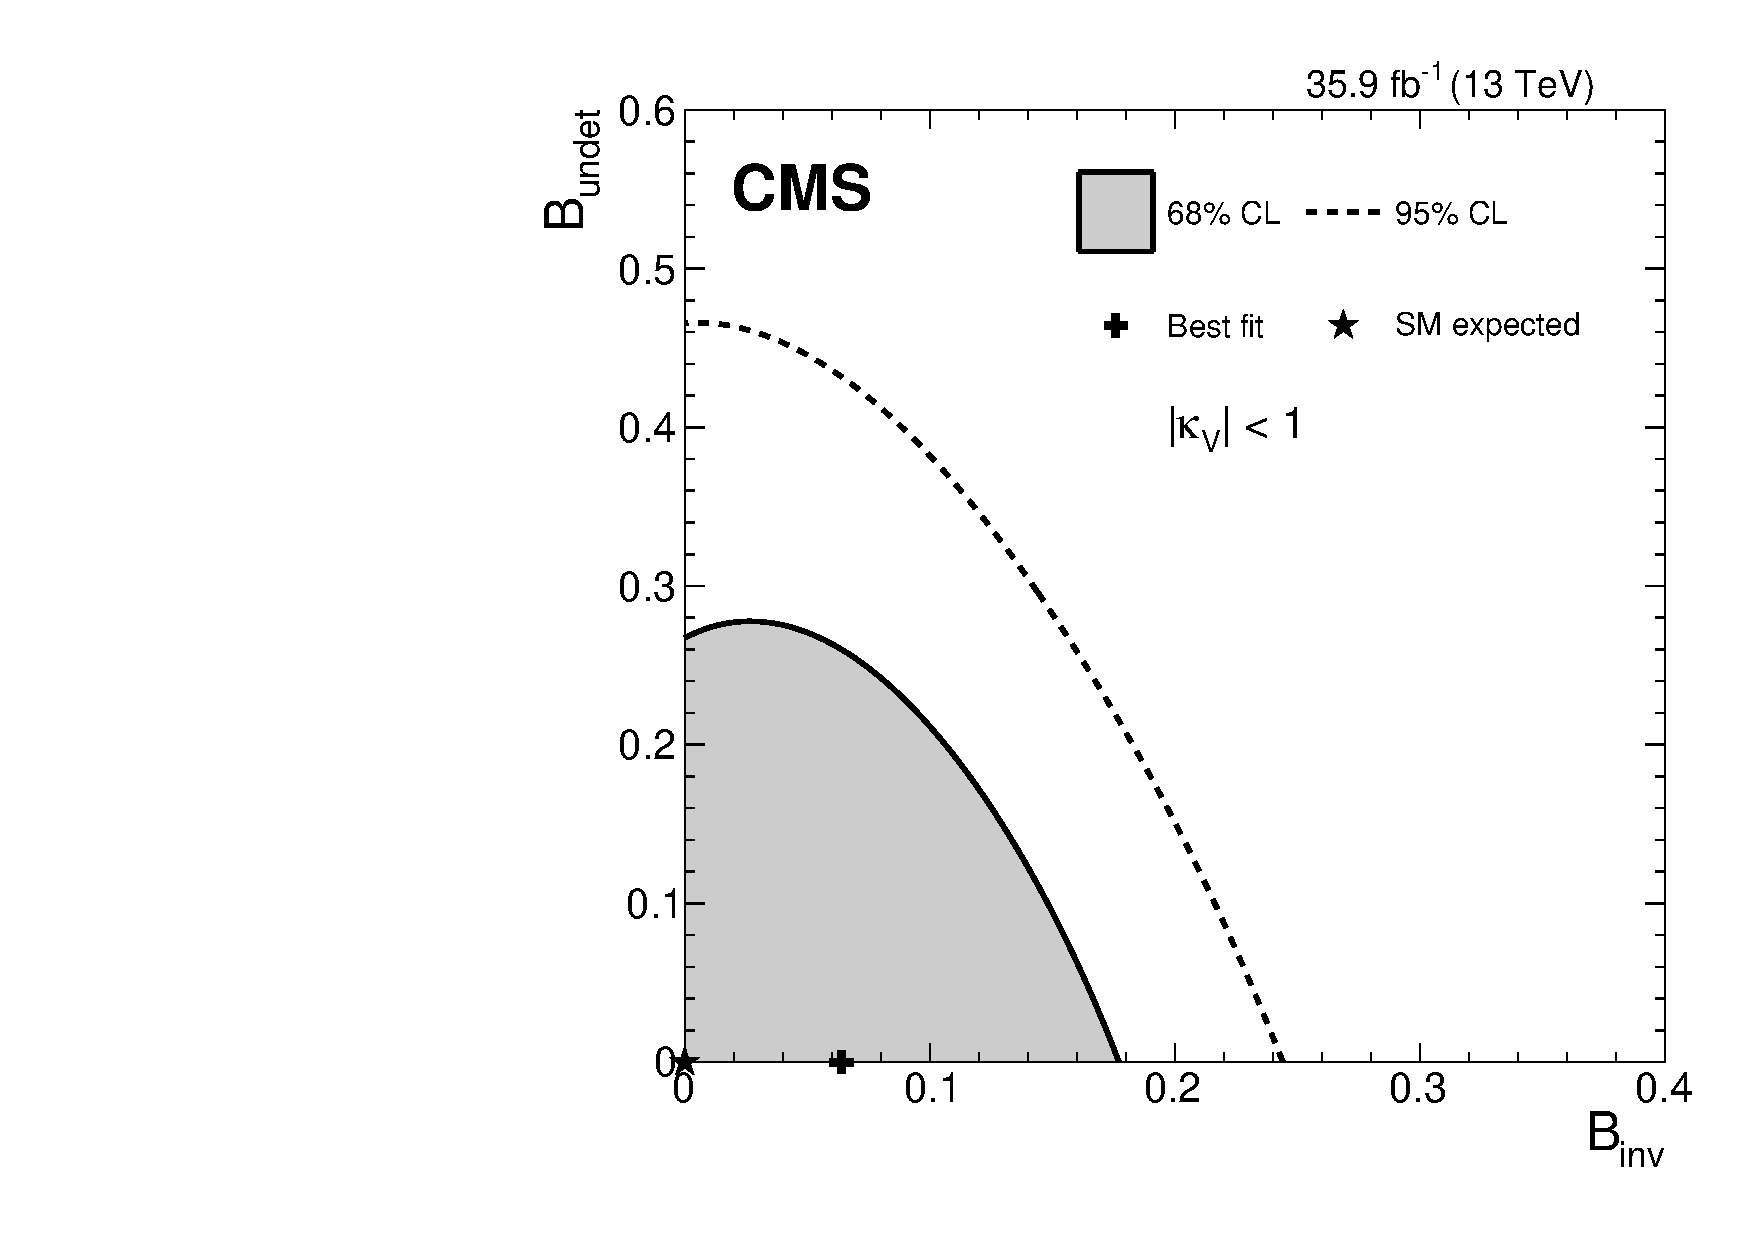
\includegraphics[width=0.465\textwidth]{Fig/HIG17031/plot_BRinvVsBRbsm_N4}\\
\caption{Scan of the test statistic as a function of $\mathcal{BR}_{\text{inv}}$ (left), and 68\% and 95\% CL regions for $\mathcal{BR}_{\text{inv}}$ vs. $\mathcal{BR}_{\text{undet}}$ (right)~\cite{CMS-PAS-HIG-17-031}. \label{fig:kappaCMS2016_3}}
\end{center}
\end{figure}

Another fit is performed using a phenomenological parameterization relating the masses of the fermions and vector bosons to the corresponding modifiers with two parameters, $M$ and $\epsilon$~\cite{Ellis:2012hz,Ellis:2013lra}. In this parametrization, the coupling modifiers, $M$ and $\epsilon$ are related as $\kappa_{F} = \frac{v\cdot m_{f}^{\epsilon}}{M^{1+\epsilon}}$ for fermions and $\kappa_{V} = \frac{v\cdot m_{V}^{2\epsilon}}{M^{1+2\epsilon}}$ for vector bosons, where $v = 246.22\GeV$ is the vacuum expectation value~\cite{Patrignani:2241948}. The SM expectation of $\kappa=1$, corresponds to $(M, \epsilon) = (v, 0)$. 
The left plot in Fig.~\ref{fig:kappaCMS2016_4} shows the $1\sigma$ and $2\sigma$ CL regions in the $(M,\epsilon)$ fit, and the results of the fit using the six modifiers are plotted versus the particle masses on the right-hand side, as well as the result of the $(M,\epsilon)$ fit. A ''reduced`` vector boson coupling $\frac{\sqrt{\kappa_{V}\cdot m_{V}}}{v}$ is shown to represent the couplings of the vector bosons in the same plot. As one can see, the couplings of these six particles to the Higgs boson are consistent within uncertainties with the SM predictions.

\begin{figure}[!ht]
\begin{center}
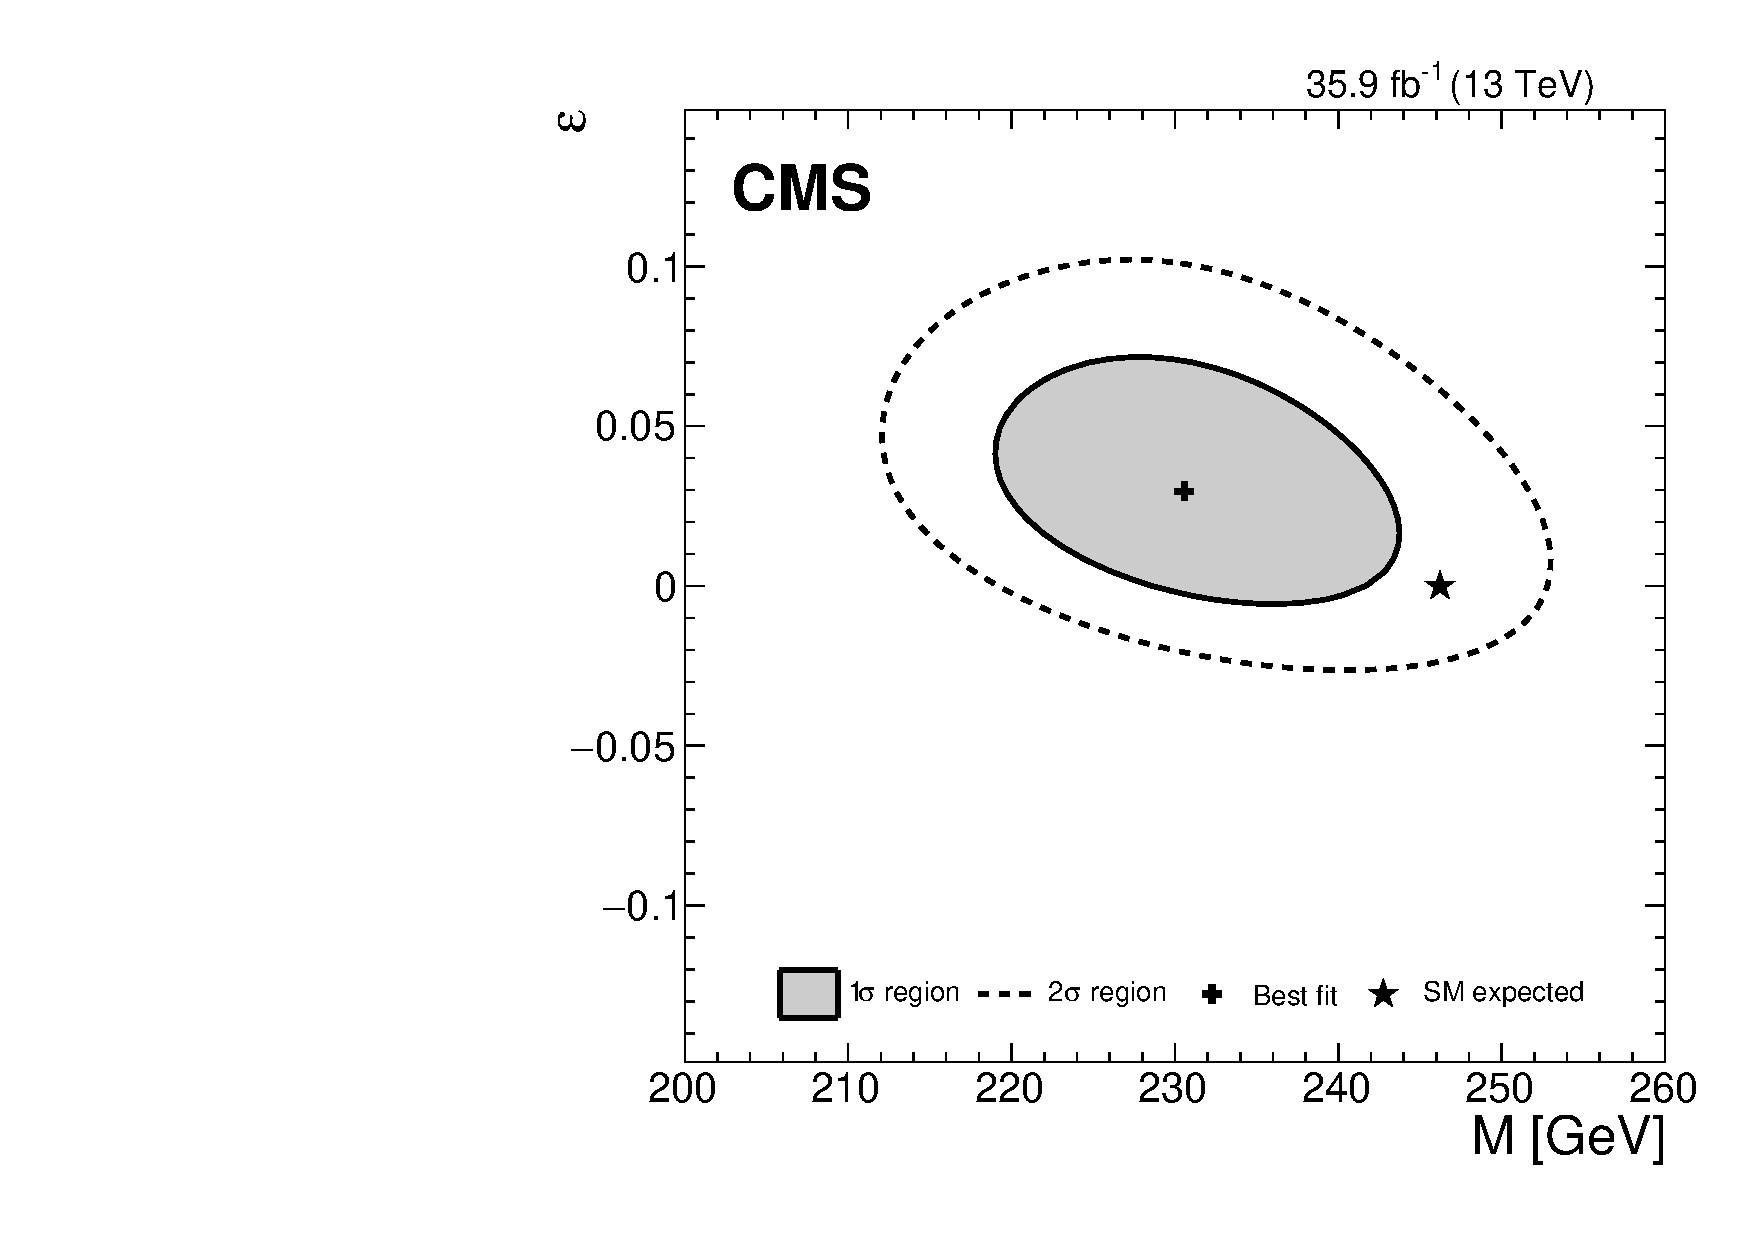
\includegraphics[width=0.5\textwidth]{Fig/HIG17031/plot_Meps_2D}~
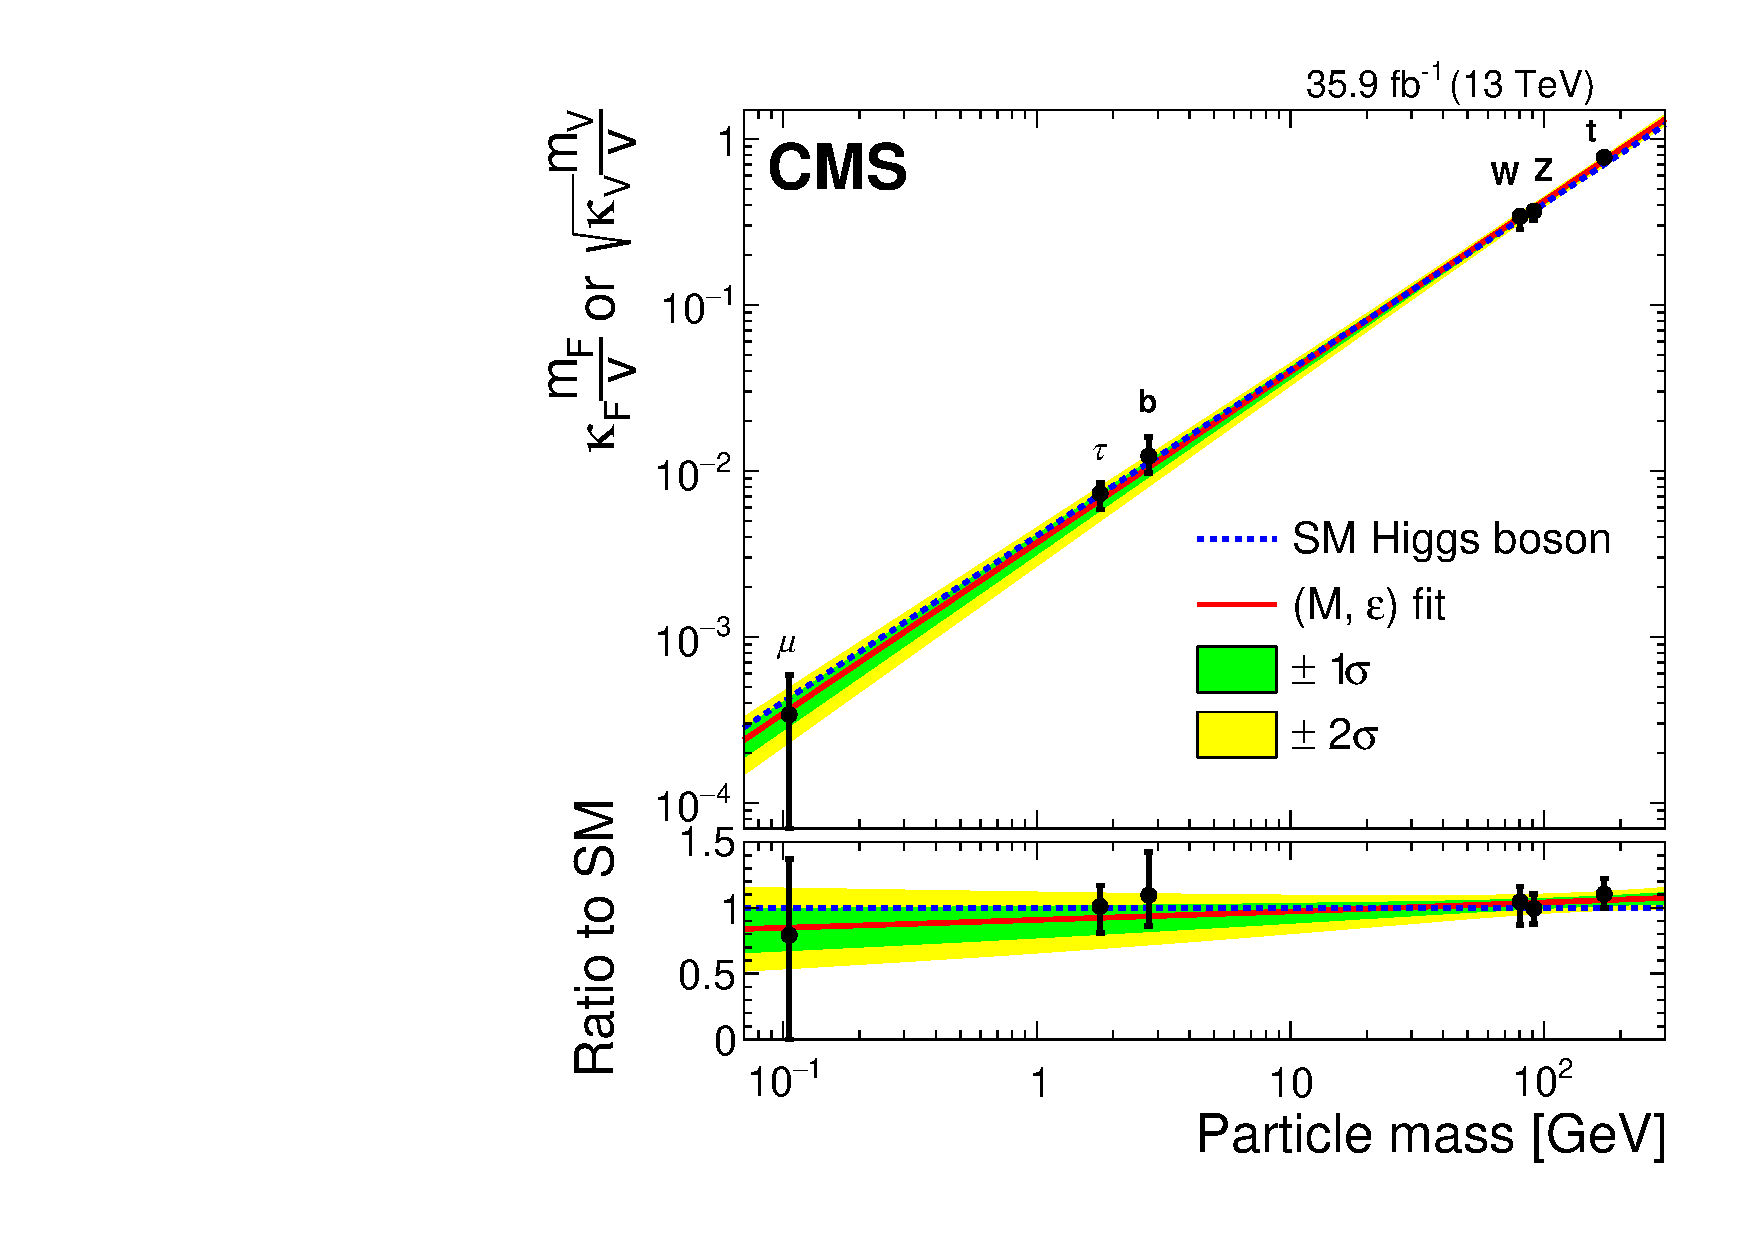
\includegraphics[width=0.5\textwidth]{Fig/HIG17031/plot_Meps_ratio}\\
\caption{(Left) Likelihood scan in the $M-\epsilon$ plane. The best fit point and the $1\sigma$ and $2\sigma$ CL regions are shown, along with the SM prediction. (Right) Result of the phenomenological $(M, \epsilon)$ fit with the loop-resolved scheme of $\kappa$-framework model~\cite{CMS-PAS-HIG-17-031}. \label{fig:kappaCMS2016_4}}
\end{center}
\end{figure}

\subsection*{The Higgs-charm coupling}
As stated previously, a sensitive measurement of Higgs-charm coupling is not feasible in the environment of the LHC. There are still ways to constrain the size of the coupling. Since c- and b-jets share rough similarities, jets originating from charm quarks may be mistagged as b- jets. Hence, with the tagging efficiency of c- and b-jets, one can recast the existing analyses of $\PH\to\bbbar$ to constrain the $\PH\to\ccbar$ rate~\cite{Perez:2015aoa}. This results in a model-independent bound on the charm signal strength of $\mu_{\cPqc}=95^{+90}_{-95}$ with the results of the $\PH\to\bbbar$ search in VH production from both ATLAS and CMS Collaborations. 
Both ATLAS and CMS Collaboration give a model-independent bound on the Higgs total width from the invariant-mass distribution of the $\PH\to\cPZ\cPZ^{*}$ and $\HGG$in the Run1 analyses. This bound on the total width can be used to constrain the Higgs-charm coupling by assuming the entire Higgs width is formed by $\PH\ccbar$. With this method, the upper bounds at 95\% CL with the CMS results is $\kappa_{\cPqc}<120$ and with the ATLAS results is $\kappa_{\cPqc}<150$. 
A method that relies on the measurements of transverse momentum distributions of Higgs boson was proposed to determine the limit on the coupling modifier $\kappa_{\cPqc}$~\cite{Bishara:2016jga}. Fig.~\ref{fig:HiggsPt_KappaC} shows the impact of the coupling modifier $\kappa_{\cPqc}$ on the normalized $p_{\text{T}}^{\PH}$ spectrum in inclusive Higgs production. This letter takes the \pt spectrum from the ATLAS combined measurement of $\HGG$ and $\PH\to\cPZ\cPZ^{*}$ decays with Run1 $\sqrt{s}=8\TeV$ data, and obtains the bounds on $\kappa_{\cPqc}$ at 95\% CL of $\kappa_{\cPqc}\in [-16,18]$. The spectrum of the $p_{\text{t}}^{\PH}$ at $\sqrt{s}=13\TeV$ is expected to be slightly harder than that of $\sqrt{s}=8\TeV$, thus will enhance the sensitivity to $\kappa_{\cPqc}$ at ongoing LHC runs as well as possible future hadron colliders at higher energies. The CMS Collaboration applies this method with the distributions from $\HGG$ and $\PH\to\cPZ\cPZ^{*}$ analyses using data collected in 2016 to set limit on the constrain of $\kappa_{\cPqc}$~\cite{CMS-PAS-HIG-17-028}. Fig.~\ref{fig:HiggsPt_KappaC_CMS2016} shows the simultaneous fit results for $\kappa_{\PQb}$ and $\kappa_{\cPqc}$. On the left plot, 1 and $2\sigma$ deviation contours for the combined ($\HGG$ and $\PH\to\cPZ\cPZ^{*}$) fit to data and for $\HGG$ and $\PH\to\cPZ\cPZ^{*}$ separately, assuming coupling dependency of the branching fractions, while the right plot assumes freely floating branching fractions in the fit. The observed (expected) constraints on $\kappa_{\cPqc}$ are
\begin{equation}
-4.3 < \kappa_{\cPqc} < 4.3\ (-5.4 < \kappa_{\cPqc} < 5.3)\ \text{(coupling dependent }\mathcal{BR}),
\end{equation}
\begin{equation}
-18.0 < \kappa_{\cPqc} < 22.9\ (-15.7 < \kappa_{\cPqc} < 19.3)\ \text{(freely floating }\mathcal{BR}).
\end{equation}
If the branching fractions are fixed to the SM expectations, the expected constraint will be
\begin{equation}
-8.7< \kappa_{\cPqc} < 10.6\ \text{(SM branching fractions)}.
\end{equation}

Rare exclusive decays of the Higgs boson to mesons in association with a photon can be used to explore these couplings. For example, the $\PH\to\JPsi\ \gamma$ decay can probe the Higgs boson coupling to the charm quark~\cite{Bodwin:2013gca}. This decay is the focus in the thesis, and will be discuss in the next section. Using Run1 results of the upper limit on $\PH\to\JPsi\ \gamma$, the bound at 95\% CL is set at $\kappa_{\cPqc}<220$.

\begin{figure}[!ht]
\begin{center}
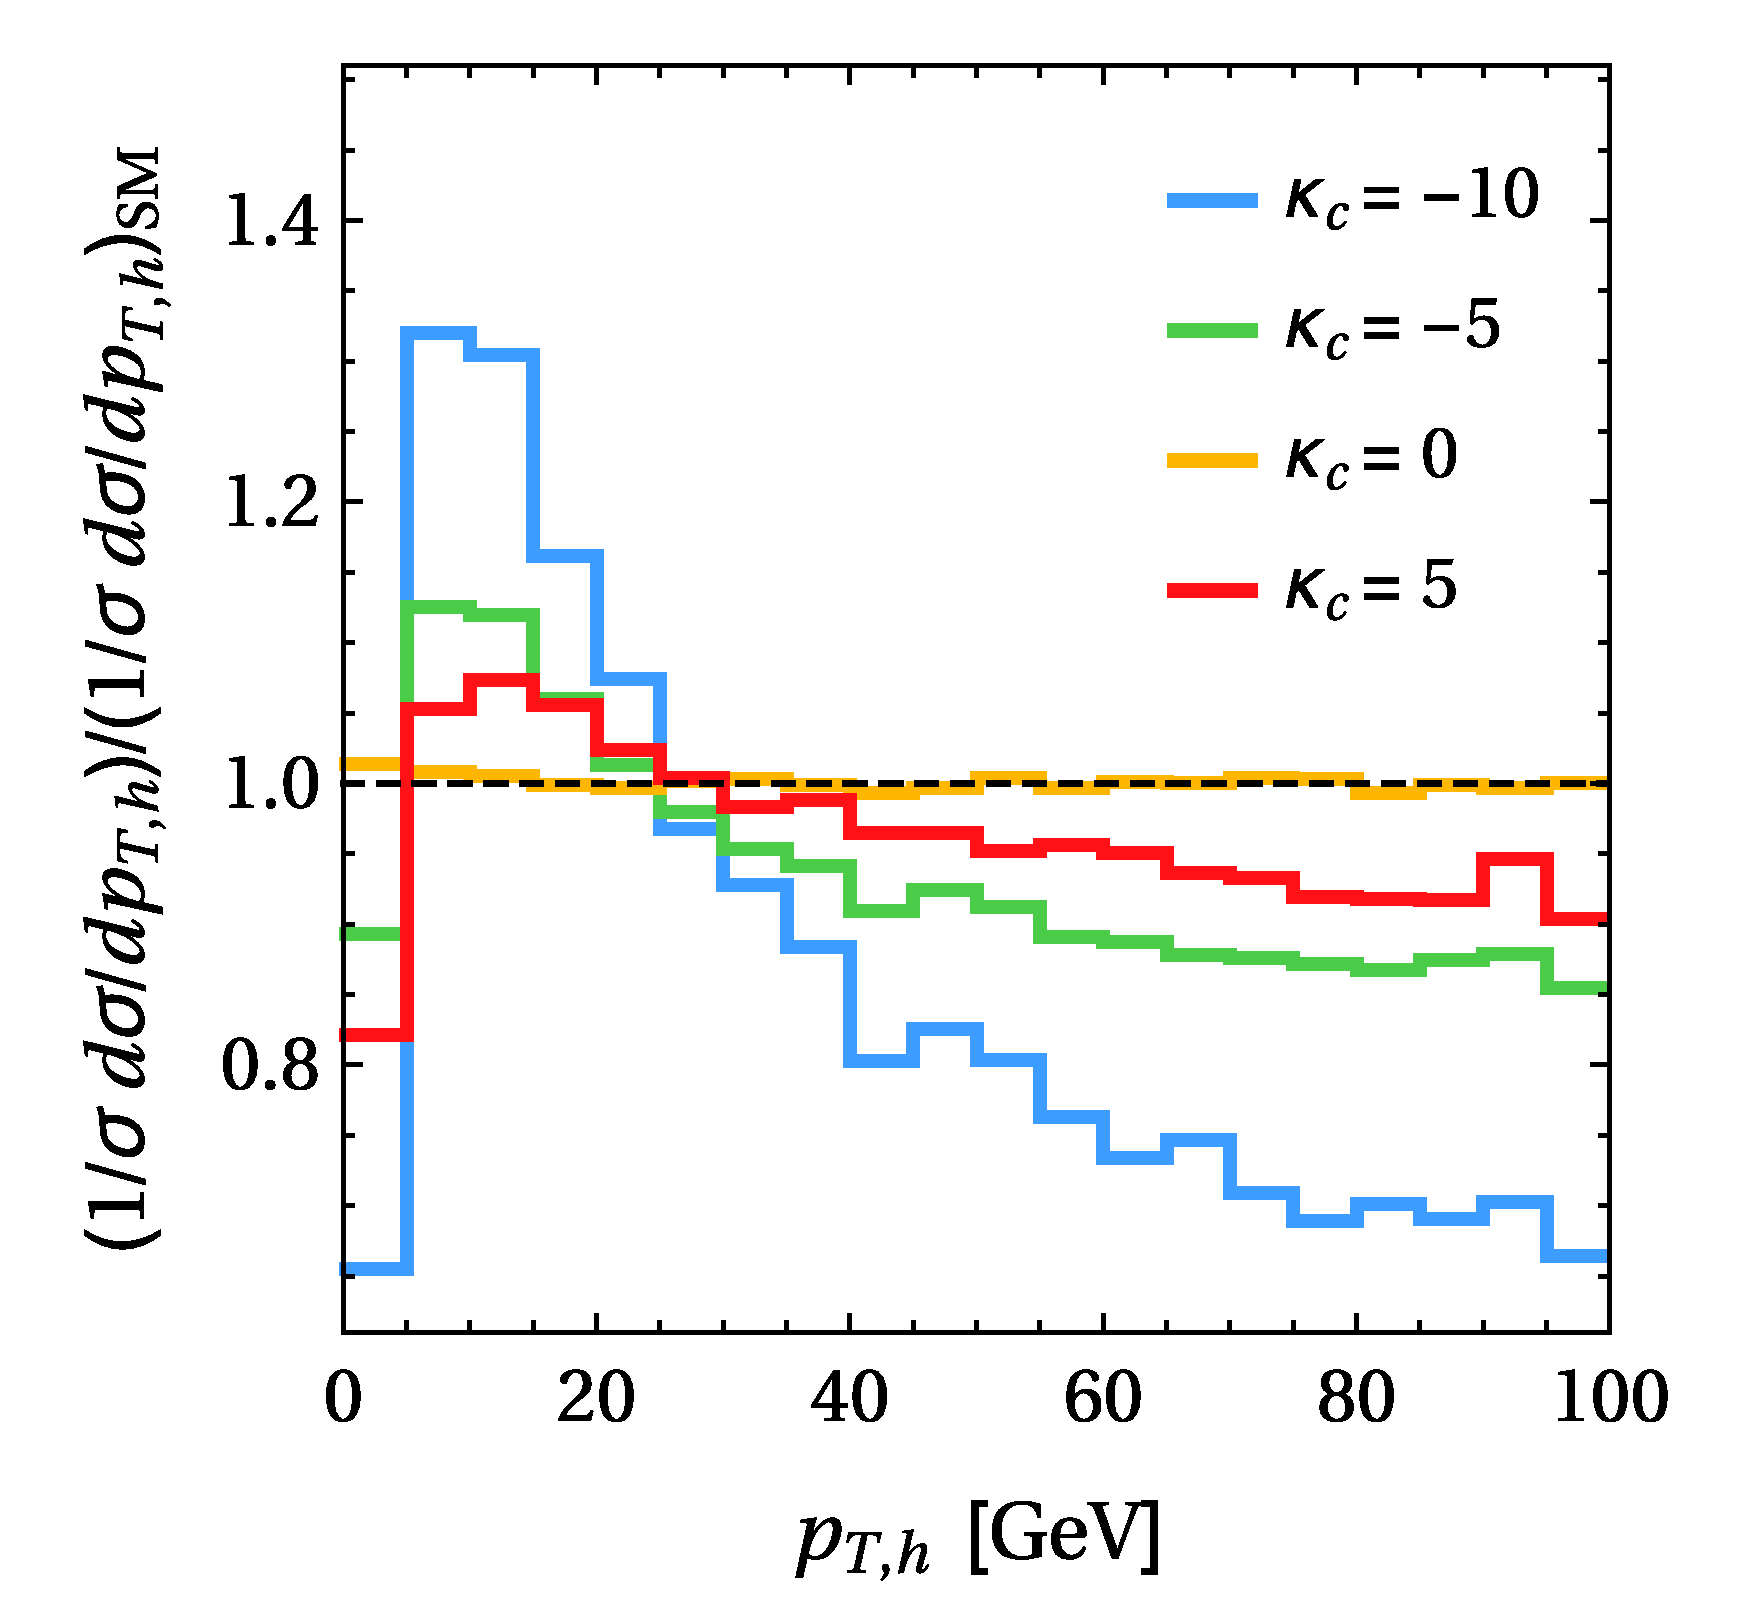
\includegraphics[width=0.5\textwidth]{Fig/HiggsPt_kappac}~
\caption{The normalized $p_{\text{T}}^{\PH}$ spectrum of inclusive Higgs production at $\sqrt{s}=8\TeV$ with different values of $\kappa_{\cPqc}$~\cite{Bodwin:2013gca}. \label{fig:HiggsPt_KappaC}}
\end{center}
\end{figure}

\begin{figure}[!ht]
\begin{center}
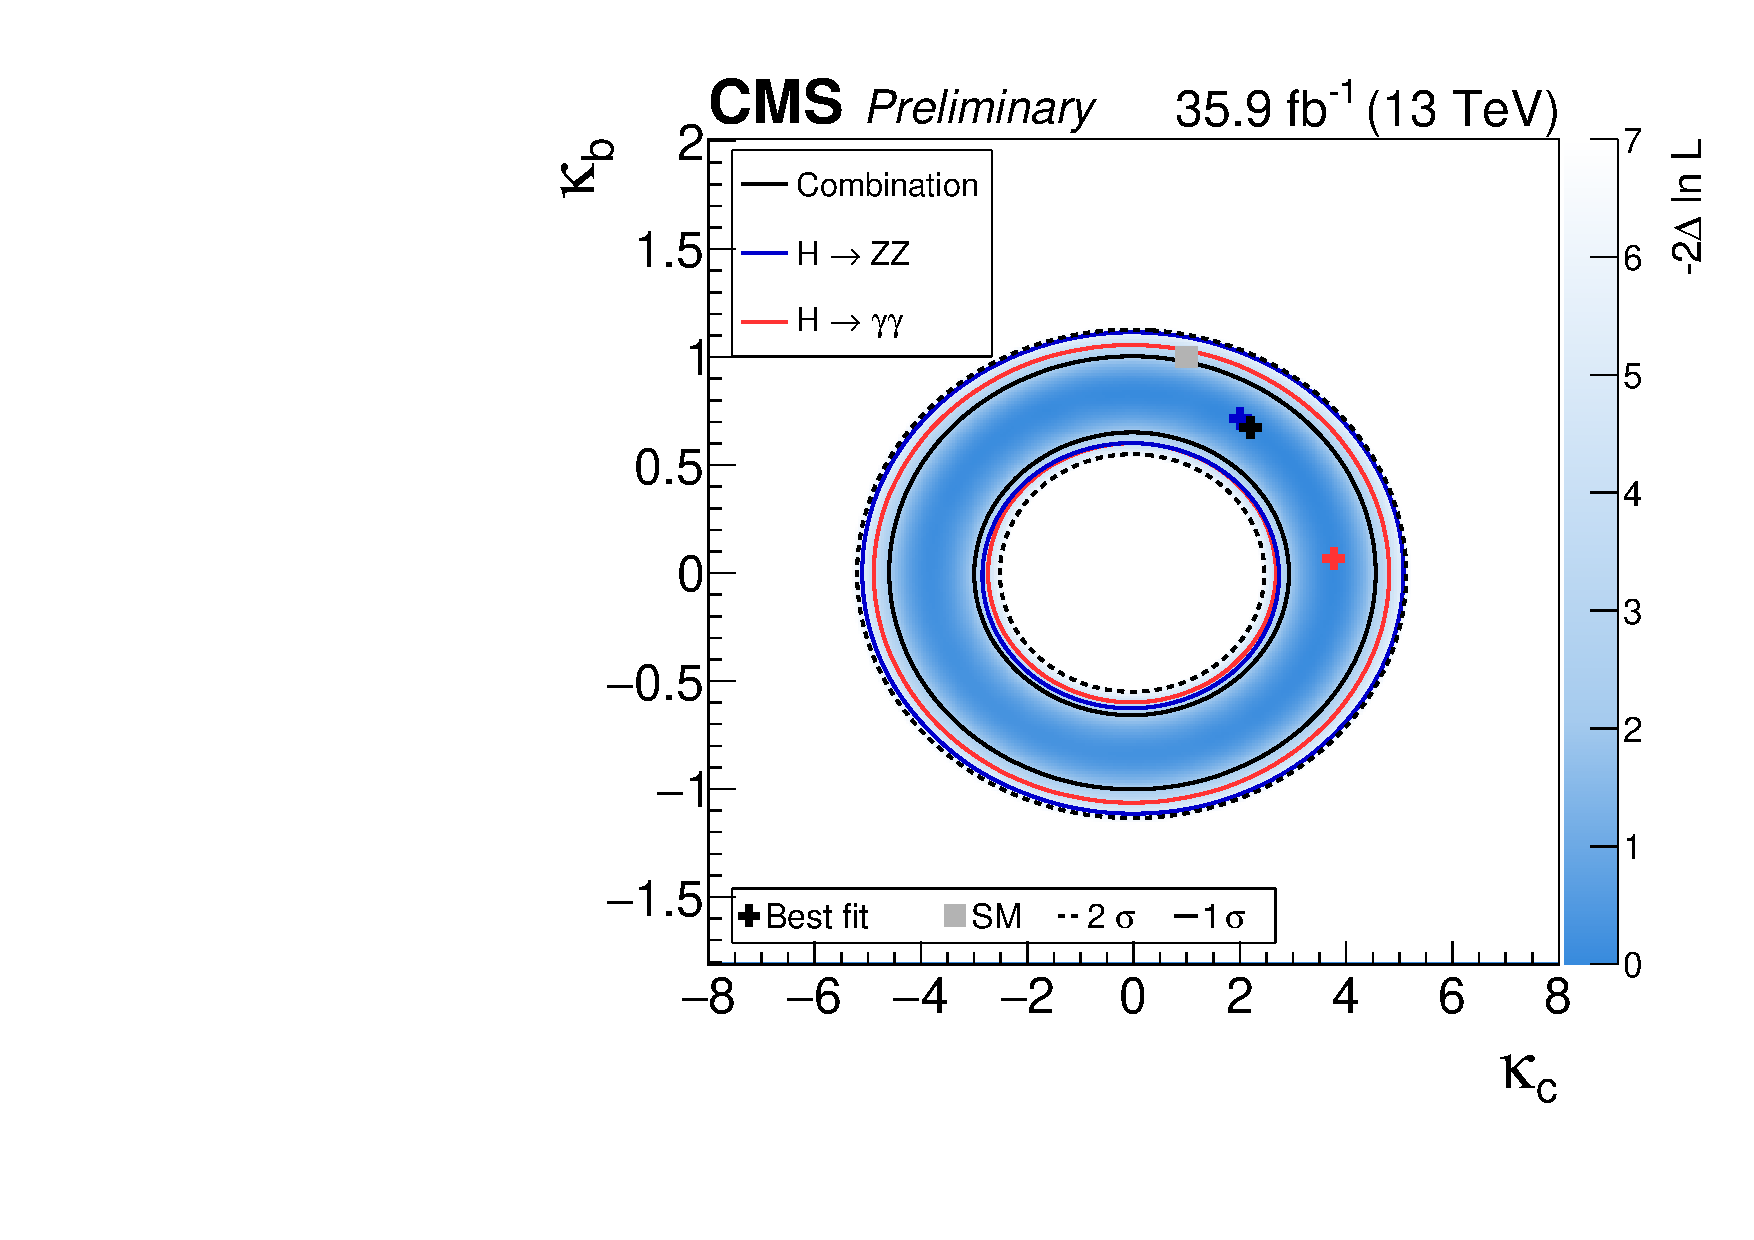
\includegraphics[width=0.5\textwidth]{Fig/CMS-PAS-HIG-17-028_Figure_006-a}~
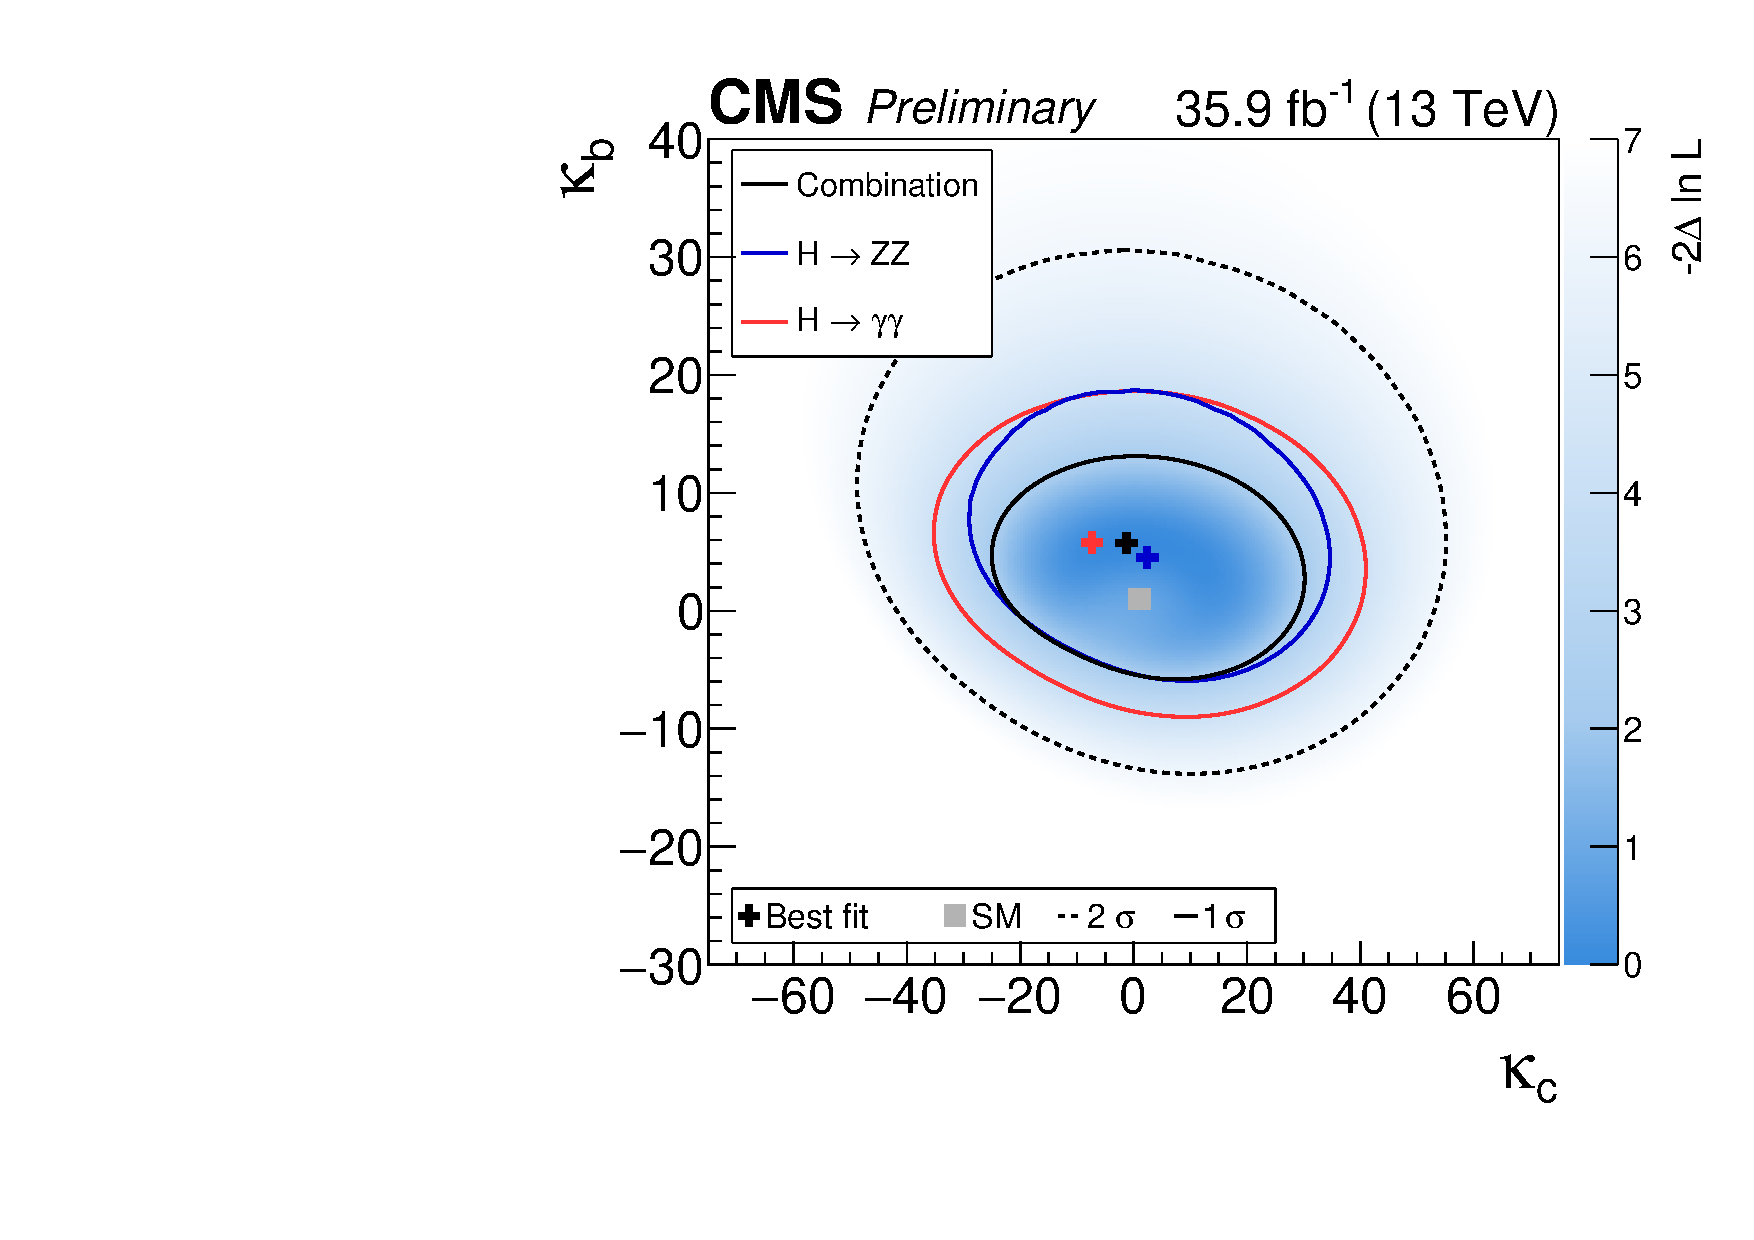
\includegraphics[width=0.5\textwidth]{Fig/CMS-PAS-HIG-17-028_Figure_006-b}\\
\caption{Simultaneous fit results for $\kappa_{\PQb}$ and $\kappa_{\cPqc}$~\cite{CMS-PAS-HIG-17-028}. \label{fig:HiggsPt_KappaC_CMS2016}}
\end{center}
\end{figure}

In some extensions to the SM, modified $\PH \ccbar$ couplings can arise~\cite{Delaunay:2013pja}. 
For example, within the context of the effective field theory~\cite{Buchmuller:1985jz,Weinberg:1980wa,Contino:2013kra} the $\PH\ccbar$ coupling is modified in the presence of dimension-six operator, leading to only an enhancement of the coupling with respect to the SM at the cutoff scale $\Lambda$, of order tens of $\TeV$, and leaving no other signature of new physics at the LHC.
In the two Higgs doublet model with minimal flavor violation~\cite{Trott:2010iz,Jung:2010ik}, the $\PH \ccbar$ coupling can be significantly enhanced by breaking the flavor symmetry, while other couplings are not severely affected. The composite pseudo-Nambu-Goldstone boson model~\cite{Giudice:2007fh} parametrizes the coupling by the degree of compositeness and compositeness scale, which can be experimentally constrained by the direct search for the charm partner~\cite{Delaunay:2013pwa}.
%In some extension theories beyond the SM, modified $\PH \ccbar$ coupling can arise~\cite{Delaunay:2013pja}. For instance, the effective field theory suggests that an enhancement of the coupling with respect to the SM can appear at cutoff scale $\Lambda$ around tens of \TeV, so that no direct signatures at the LHC can be observed other than a significantly enhanced $\PH \ccbar$ coupling. In the two Higgs doublet model with minimal flavor violation~\cite{Trott:2010iz,Jung:2010ik}, the $\PH \ccbar$ coupling can be significantly enhanced by breaking the flavor symmetry, while other couplings not severely affected. The composite pseudo-Nambu-Goldstone boson model~\cite{Giudice:2007fh} parametrizes the coupling by the degree of compositeness and compositeness scale, which can be experimentally constrained by the direct search of the charm partner~\cite{Delaunay:2013pwa}.

\section{The rare decays $\cPZ/\PH\to\JPsi\ \gamma$}
\subsection{Overview}
%A new boson with a mass of approximately 125\GeV was discovered by the ATLAS and CMS Collaborations at the CERN LHC in 2012~\cite{Chatrchyan2013,Aad:2013xqa,201230,Chatrchyan:2013lba,CMS:2014ega,AtlasProperties,CMS:2015kwa}. 
%Up to now, all measurements of its properties are consistent with those of the Higgs boson of the SM. 
%The Higgs boson Yukawa couplings to the first-- and second--generation quarks are currently weakly constrained.
%Rare exclusive decays of the Higgs boson to mesons in association with a photon can be used to explore these couplings. For example, the $\PH\to\JPsi\ \gamma$ decay can probe the Higgs boson coupling to the charm quark~\cite{Bodwin:2013gca}.
The rare decay of $\PH\to\JPsi\ \gamma$ is one of the proposed ways to probe the Higgs-charm coupling. The corresponding decay of the $\cPZ$ boson, $\cPZ\to\JPsi\ \gamma$, can be used as an experimental benchmark for the $\PH\to\JPsi\ \gamma$ search, given that the mass of the $\cPZ$ boson is not far from that of the Higgs boson, and to test various QCD factorization approaches that are being used in the estimation of branching fractions for hadronic radiative decays of bosons~\cite{GUBERINA1980317,PhysRevD.92.014007,Grossmann:2015lea}.

Both the Higgs and $\cPZ$ boson decays have contributions from direct and indirect processes. In the direct mechanism, $\cPZ$ and Higgs bosons couple to charm quarks, and charm quarks then hadronize to form $\JPsi$ mesons. 
In the indirect mechanism, the Higgs and $\cPZ$ bosons decay through the quark and W boson loops to 
$\gamma\gamma^{*}$, and the $\gamma^{*}$ then converts to a $\ccbar$ resonant state.  
The Feynman diagrams for these decay modes are shown in Fig.~\ref{fig:ZJpsiG_diag}. 
The widths of the decays are expected to be
\begin{equation}
\label{eqn:widthHJpsiG}
\begin{split}
\Gamma_{\PH\to\JPsi\ \gamma} & =\frac{1}{8\pi}\frac{m_{\PH}-m_{\JPsi}}{m_{\PH}} |\mathcal{A}_{\text{direct}}+\mathcal{A}_{\text{indirect}}|^{2} \\
& = \bigg[(11.71\pm 0.17) - \big[(0.659^{+0.085}_{-0.085})+i(0.073^{+0.035}_{-0.035})\big]\kappa_{\cPqc}\bigg]\ten{-10}\GeV \\
& =1.221^{+0.042}_{-0.041}\ten{-8}\GeV,
\end{split}
\end{equation}
\begin{equation}
\label{eqn:widthZJpsiG}
\Gamma_{\cPZ\to\JPsi\ \gamma}=\frac{m_{\cPZ}^{3}}{96\pi m_{\JPsi}^{2}} |\mathcal{A}_{\text{direct}}+\mathcal{A}_{\text{indirect}}|^{2}= 2.236^{+0.377}_{-0.344}\ten{-7}\GeV,
\end{equation}
where in Eq.~\ref{eqn:widthHJpsiG} the equality and numerical results are taken from Ref.~\cite{Bodwin:2013gca,Bodwin:2017wdu}, and those in Eq.~\ref{eqn:widthZJpsiG} are from Ref.~\cite{Bodwin:2017pzj}.
In these theoretical calculations, a framework of the nonrelativistic QCD (NRQCD) factorization~\cite{PhysRevD.51.1125} is used, where the nonperturbative effects are parametrized in terms of the quarkonium light-cone distribution amplitudes (LCDAs)~\cite{PhysRevD.22.2157,Chernyak:1983ej}. These computations will not be discussed in detail here. 
With the total widths of both the Higgs $\Gamma_{\PH}=4.20\MeV$ and $\cPZ$ boson $\Gamma_{\cPZ}=2.4952\GeV$ and $\kappa_{\cPqc}=1$ in the SM, the branching fractions of both decays are then:
\begin{equation}
\mathcal{B}_{\text{SM}}(\PH\to\JPsi\ \gamma)=(3.0^{+0.2}_{-0.2})\ten{-6}.
\end{equation}
\begin{equation}
\mathcal{B}_{\text{SM}}(\cPZ\to\JPsi\ \gamma)=(9.0^{+1.5}_{-1.4})\ten{-8},
\end{equation}
The direct and indirect amplitudes interfere destructively in both decays. In the Higgs decay, the contribution from the indirect process is larger. Only direct process included in the calculation leads to a brancing fractions of $5.28\ten{-8}$, while only indirect diagrams included results in a brancing fractions of $3.25\ten{-6}$. The branching fraction of the $\cPZ$ decay, compared to the Higgs decay, is smaller by 1-2 orders of magnitude. This results from the suppression of the indirect amplitude, which is less than 1\% of the magnitude of direct amplitude, in the $\cPZ$ decay. One qualitative explanation uses the Landau-Yang theorem~\cite{PhysRev.77.242}, which states that the $\cPZ$ boson does not decay to two on-shell photon. This requires that the indirect amplitude tends to zero in the limit $m_{\JPsi}\to 0$.

With the branching fractions shown above, one can obtain
\begin{equation}  
\begin{split}
\sigma(\Pp\Pp\to\PH) \times \mathcal{B}_{\text{SM}}&(\PH\to\JPsi\ \gamma\to\mu\mu\gamma) = \\
& 55\ \text{pb} \times 3.0\times10^{-6} \times 0.059 = 9.8\ten{-3}\ \text{fb},
\end{split}
\end{equation}  
\begin{equation} 
\begin{split}
\sigma(\Pp\Pp\to\cPZ) \times \mathcal{B}_{\text{SM}}&(\cPZ\to\JPsi\ \gamma\to\mu\mu\gamma) =\\
& 5.7\times 10^{4}\ \text{pb} \times 9.0\times10^{-8} \times 0.059 = 3.0\ten{-1}\ \text{fb}.
\end{split}
\end{equation}
where the cross-section of the Higgs boson are summed over the ggF, VBF, VH, and ttH productions, and taken from Ref.~\cite{deFlorian:2016spz}. The cross-section of the $\cPZ$ boson are calculated using $\FEWZ$ 3.1.b2 program~\cite{Li:2012wna}.

\begin{figure}[!ht]\begin{center}
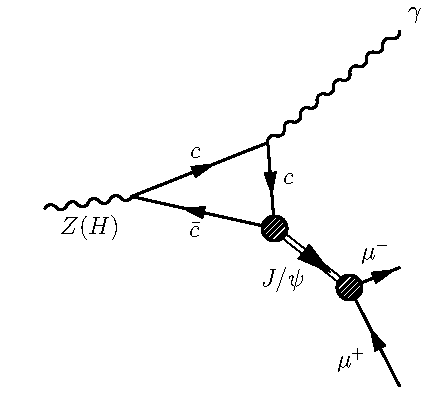
\includegraphics[width=0.4\textwidth]{Fig/ZJpsiG_direct_v2}\\
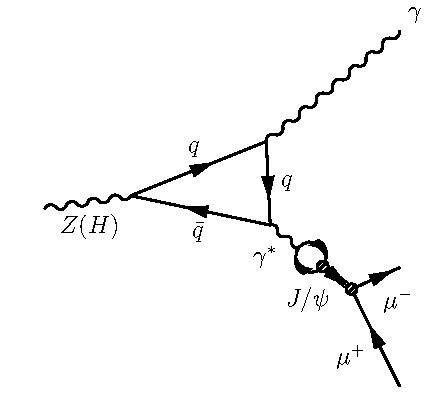
\includegraphics[width=0.33\textwidth]{Fig/ZJpsiG_Indirect1_v2}~
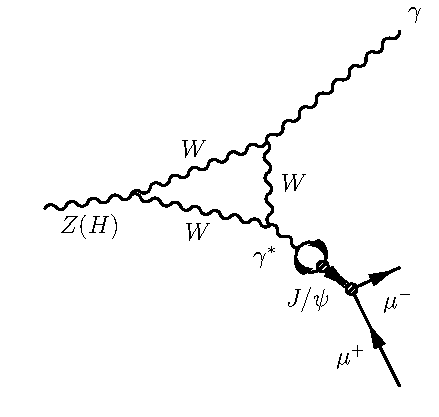
\includegraphics[width=0.33\textwidth]{Fig/ZJpsiG_Indirect2_v2}~
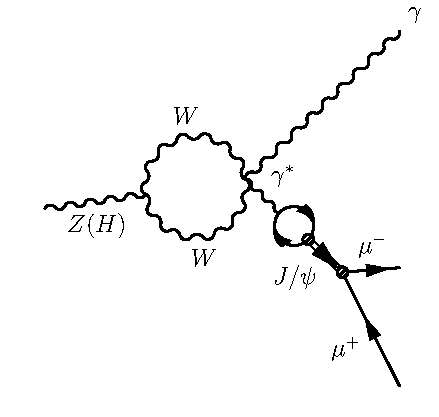
\includegraphics[width=0.33\textwidth]{Fig/ZJpsiG_Indirect3_v2}\\
\caption{Feynman diagrams for $\cPZ(\PH)\to\JPsi\ \gamma$ decay. The top diagram shows the direct process and the remaining diagrams show the indirect processes.}
\label{fig:ZJpsiG_diag}\end{center}\end{figure}

Deviations from the SM predictions for the couplings can affect the interference terms and may result in changes in the branching fractions. 
For example, the shift in the branching fraction for $\PH\to\JPsi\ \gamma$ can be more than 100\% if the $\PH \ccbar$ coupling deviates from its SM value by more than a factor of 2, as shown in Fig.~\ref{fig:BRShift}. 
Measurements of the direct decay of $\PH\to\ccbar$ leave the overall signs of the couplings undetermined. This ambiguity can be resolved by the interference terms in $\PH\to\JPsi\ \gamma$, providing us with additional information about the Higgs properties.
%Since this Higgs boson decay is sensitive to the $\PH\ccbar$ coupling, a measurement of the branching fraction can verify if the Higgs boson couples to second-generation quarks with the strength predicted by the SM.

\begin{figure}[!ht]
  \begin{center}  
    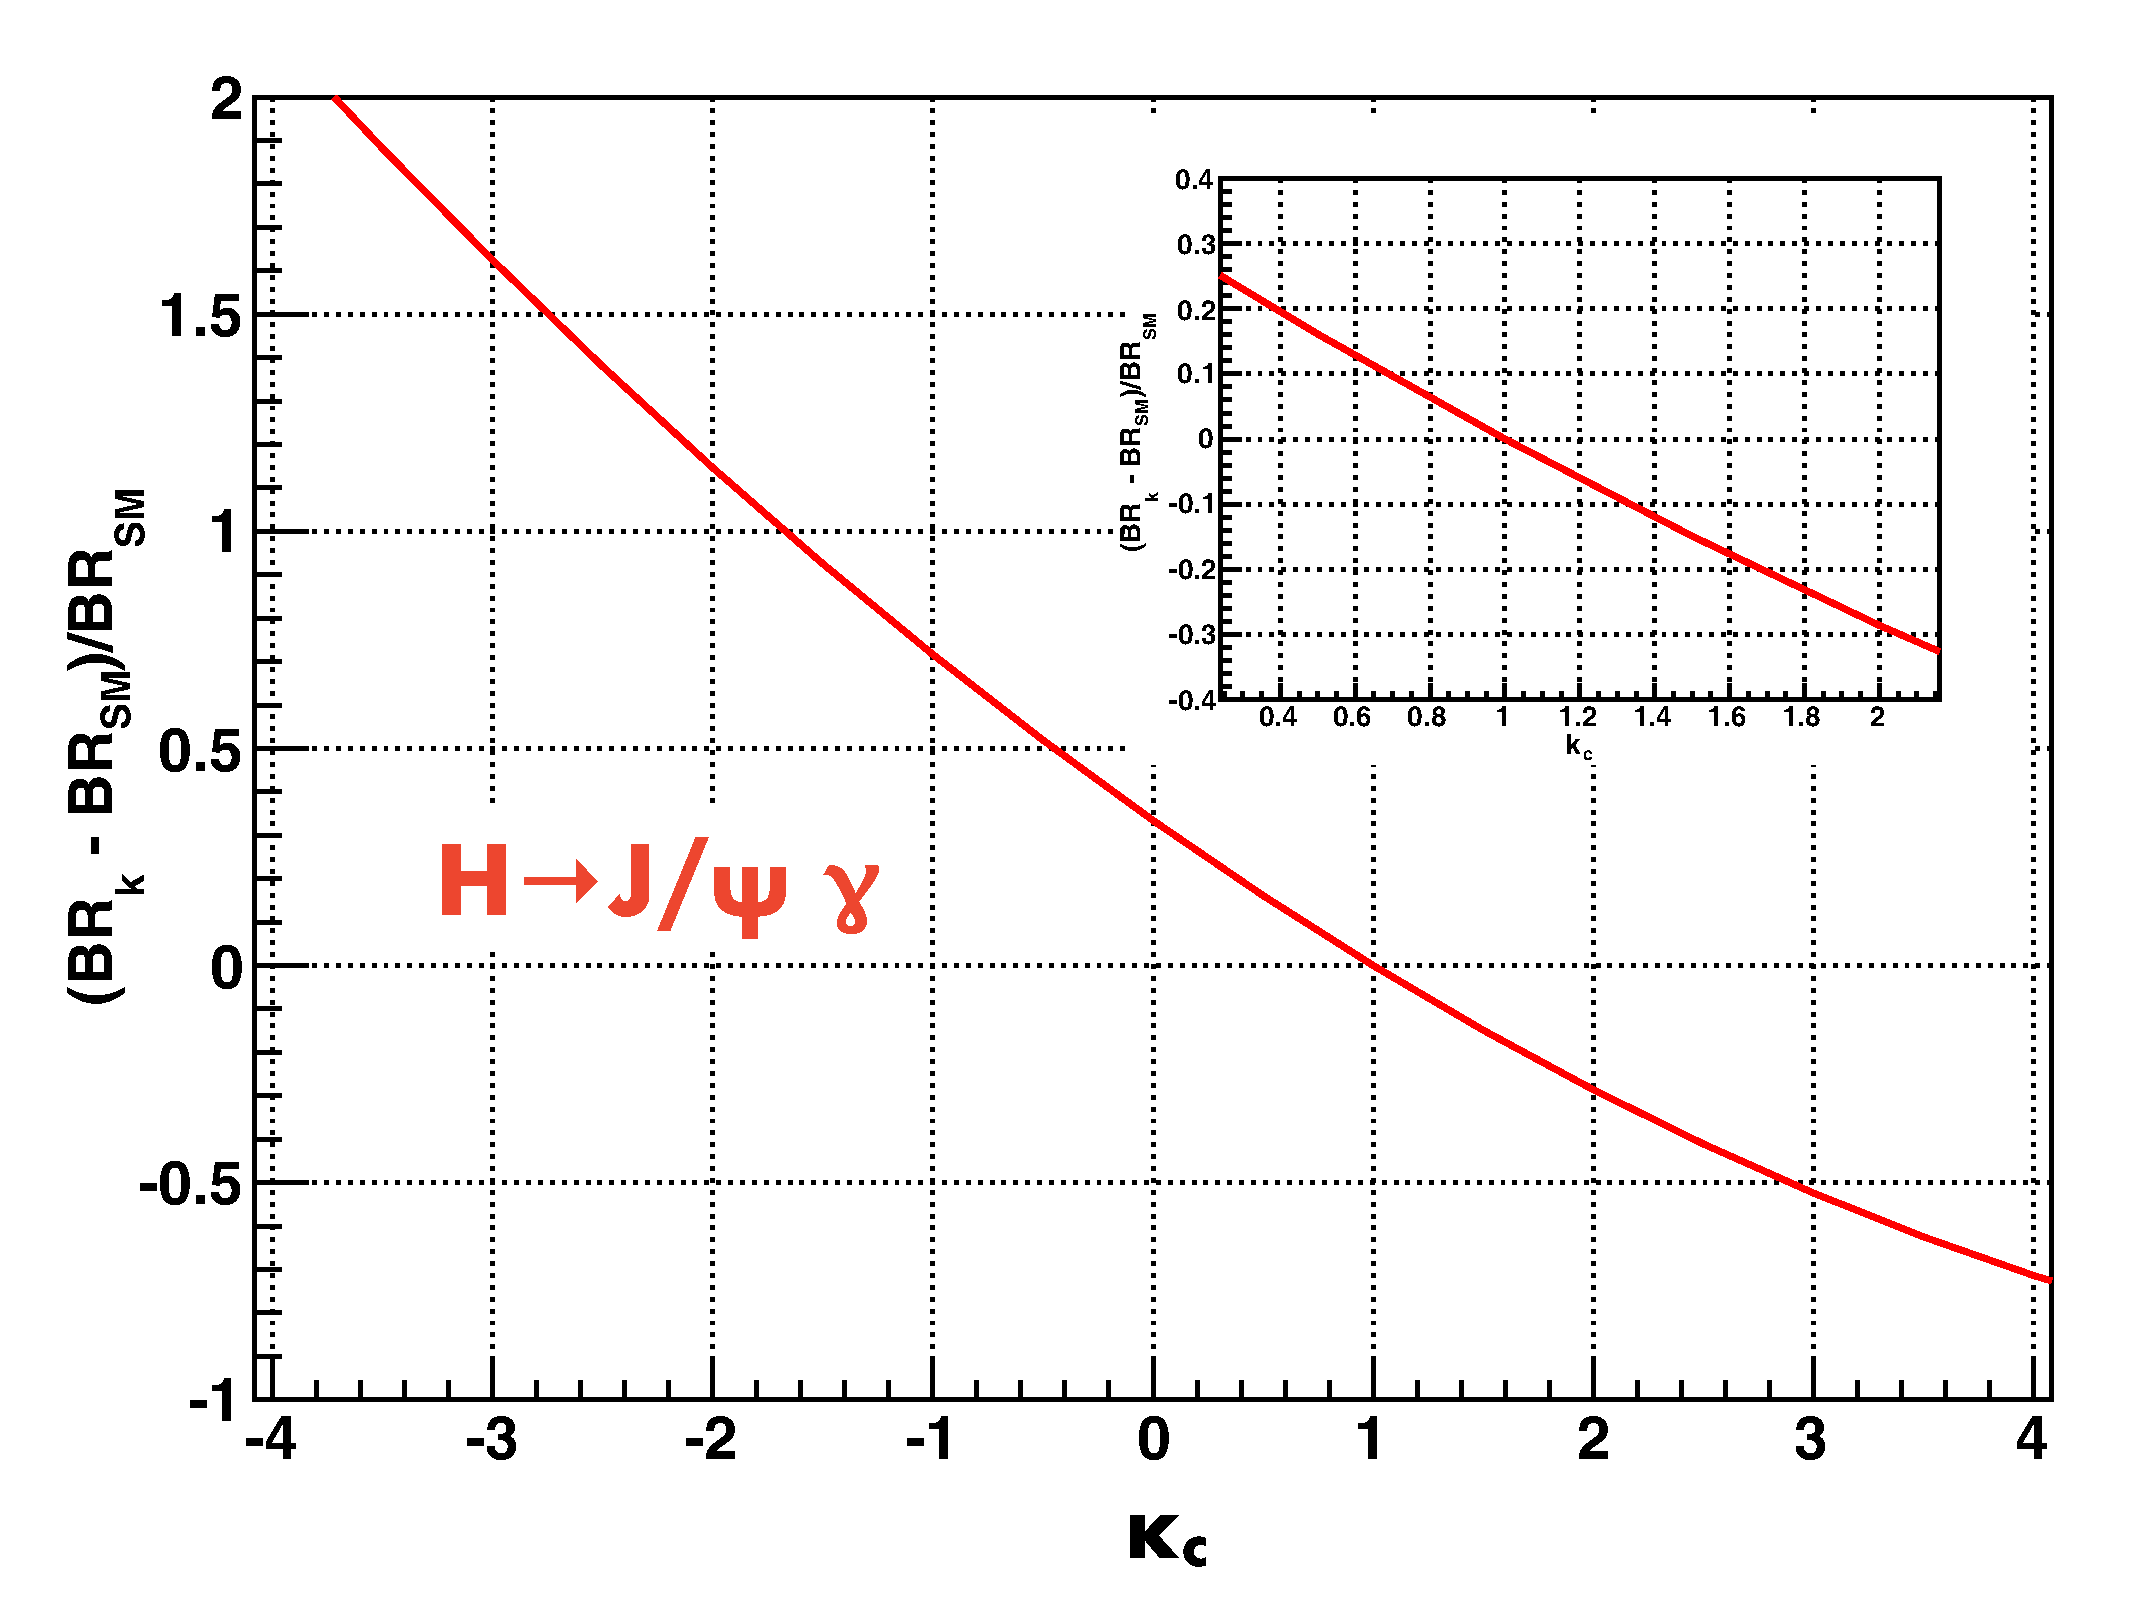
\includegraphics[width=0.65\textwidth]{Fig/BRShift}\\
    \caption{The relative deviations in the branching fraction for $\PH\to\JPsi\ \gamma$ as function of $\kappa_{\cPqc}$~\cite{Bodwin:2013gca}.  \label{fig:BRShift}}  
  \end{center}
\end{figure}

%\begin{figure}[!ht]
%  \begin{center}  
%    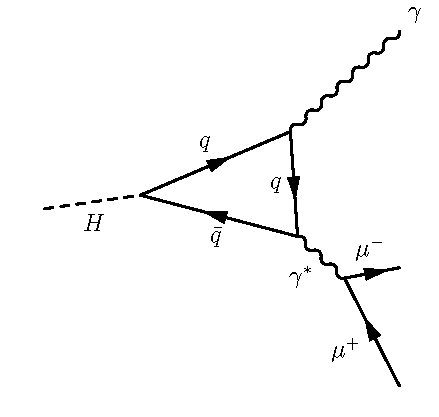
\includegraphics[width=0.35\textwidth]{Fig/HDalitz_1}~
%    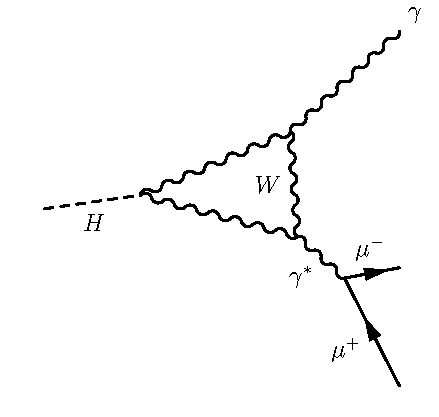
\includegraphics[width=0.35\textwidth]{Fig/HDalitz_2}\\
%    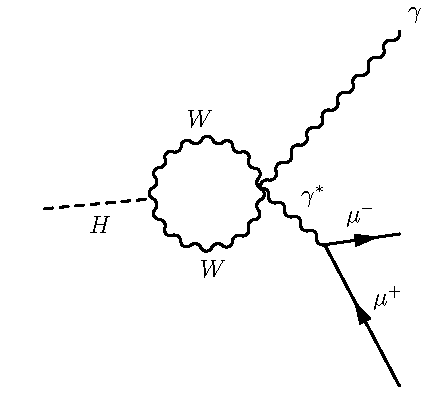
\includegraphics[width=0.35\textwidth]{Fig/HDalitz_3}\\
%    \caption{Main diagrams for the Higgs Dalitz decay, $\PH\to\gamma^{*}\gamma\to\mu\mu\gamma$}  
%    \label{fig:FeynmanDiagrams_Dalitz}
%  \end{center}
%\end{figure} 
%
%
%\begin{figure}[!ht]
%  \begin{center}  
%    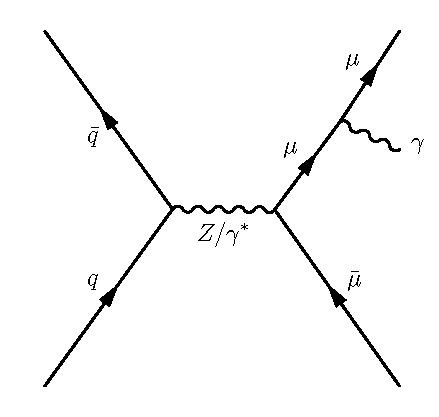
\includegraphics[width=0.35\textwidth]{Fig/Zmmg1}~
%    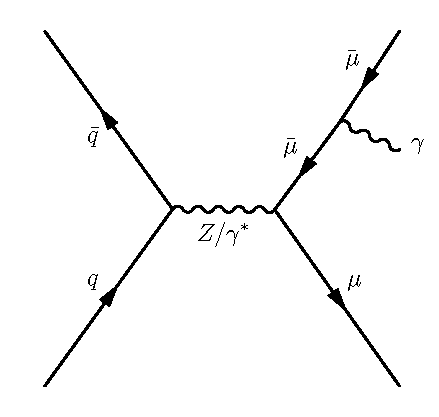
\includegraphics[width=0.35\textwidth]{Fig/Zmmg2}
%    \caption{Main diagrams for the Drell-Yan process, $\Pp\Pp\to\cPZ\to\mu\mu\gamma$, which is the background that will exhibit a peak in $\text{m}_{\mu\mu\gamma}$ at the Z boson mass, $m_{\cPZ}$.}  
%    \label{fig:FeynmanDiagrams_Zmmg}
%  \end{center}
%\end{figure}

\subsection{Features of the decays}
Due to the relatively heavy $\cPZ$ and Higgs boson, the $\JPsi$ and $\gamma$ from their decays will have high transverse momenta $\pt$ and energy $\et$ (boosted). The high-$\et$ photon will be produced back-to-back to the $\JPsi$ particle, and hence can be distinguished from backgrounds easily and be identified as an isolated photon. 
Since the $\JPsi$ meson from $\cPZ$ (Higgs) boson decay is boosted, the $\pt$ of the two muons from its decay are anti-correlated. Further, these two muons are very close to each other spatially. Therefore, dedicated strategies for trigger algorithms and both offline reconstruction are needed. 
The photon should be well separated from each muon. This event signature can be utilized to design kinematic requirements such as the angular separation $\Delta R$\footnotemark to reject backgrounds. 
\footnotetext{The coordinate system will be introduced in the next chapter.}

%The background compositions are not complicated. The main irreducible background is the Drell-Yan process, where the photon can either be initial-state radiation (ISR) or final-state radiation (FSR). The reducible backgrounds come from Drell-Yan with jet and inclusive quarkonium production, where the jet in both processes is misidentified as a photon at reconstruction level. 
%$\JPsi$ mesons can come from heavy-flavor hadron decays (These $\JPsi$ mesons will be referred to as non-prompt $\JPsi$). 
%Those $\JPsi$ mesons have longer proper decay time $t$ and decay length $\text{L}_{\text{xy}}$ than those of the $\JPsi$ meson from signal events (The $\JPsi$ from the signal events are therefore called prompt $\JPsi$). 
%These features can be used to examine if the reconstructed $\JPsi$ meson candidate in selected events are promptly produced.  

Fig.~\ref{fig:GenLevel_HJpsiG} shows the distributions of key variables at the generator level. All the distributions shown in the figure are normalized to unity. One can see that, the momenta of muons cover a wide range: the transverse momentum \pt of trailing muon\footnotemark can be less than 10\GeV, while that of leading muon can be greater than 40 and 60\GeV in the $\cPZ$ and Higgs boson decay respectively. The photon can have high transverse energy. The muons and the photon distribute mostly in the central region. The high-$\et$ photon is back-to-back to the dimuon system, while the two muons are close to each other spatially. 
\footnotetext{In the analysis, two muons will be selected in the final state. The one with higher \pt is referred to as leading muon, and the other one is then referred to as trailing or subleading muon.}

\begin{figure}[p]\begin{center}  
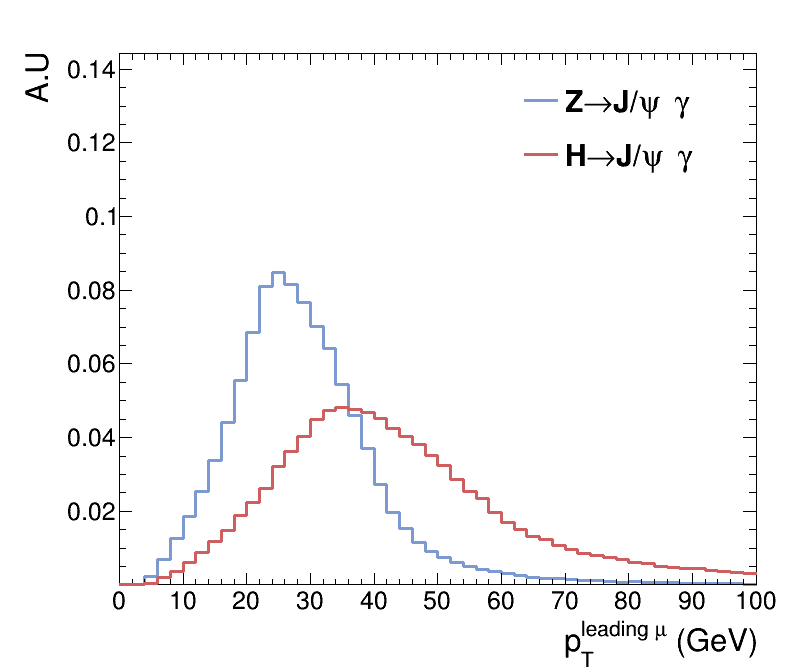
\includegraphics[width=0.33\textwidth]{Fig/GenLevel_HJpsiG/plot_ZHJpsiG/ZHJpsiG_mu1Pt}~
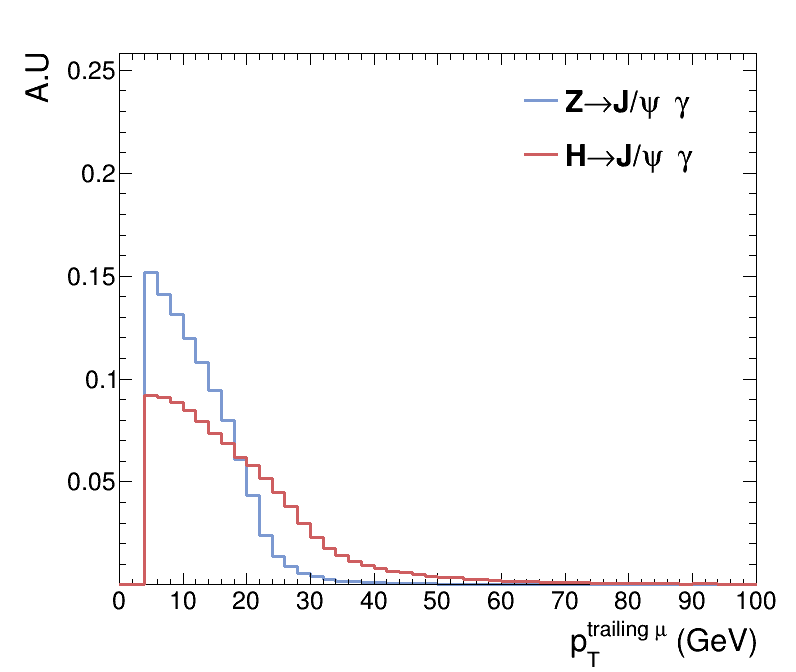
\includegraphics[width=0.33\textwidth]{Fig/GenLevel_HJpsiG/plot_ZHJpsiG/ZHJpsiG_mu2Pt}~
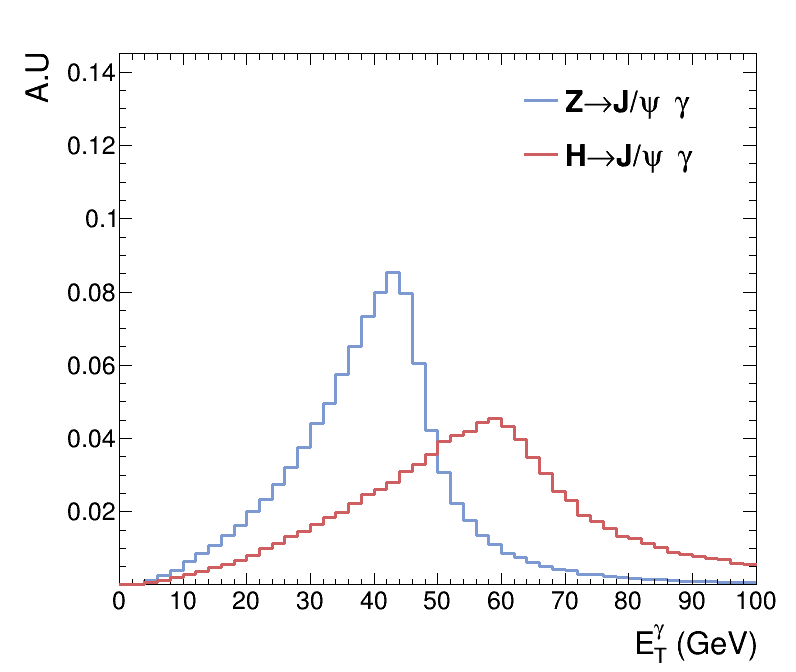
\includegraphics[width=0.33\textwidth]{Fig/GenLevel_HJpsiG/plot_ZHJpsiG/ZHJpsiG_phoEt}\\
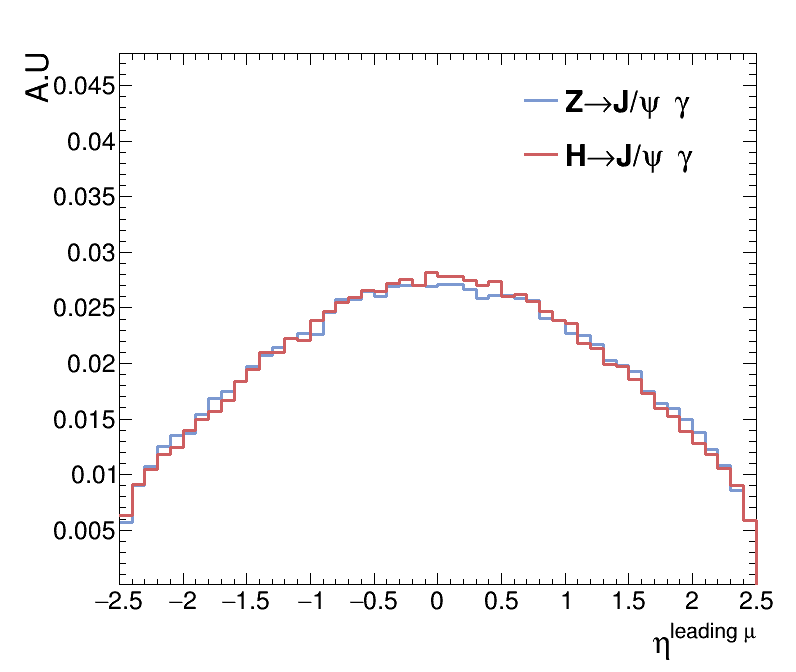
\includegraphics[width=0.33\textwidth]{Fig/GenLevel_HJpsiG/plot_ZHJpsiG/ZHJpsiG_mu1Eta}~
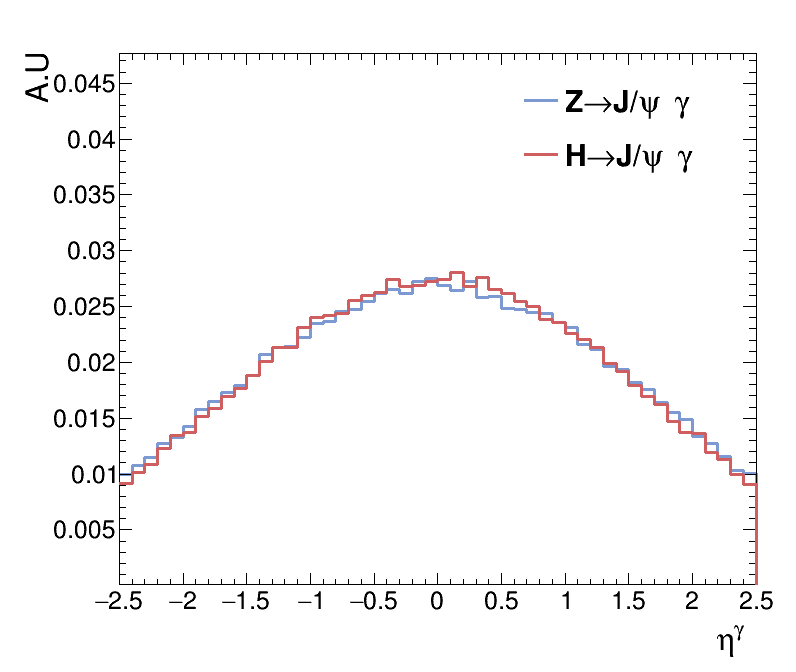
\includegraphics[width=0.33\textwidth]{Fig/GenLevel_HJpsiG/plot_ZHJpsiG/ZHJpsiG_phoEta}~
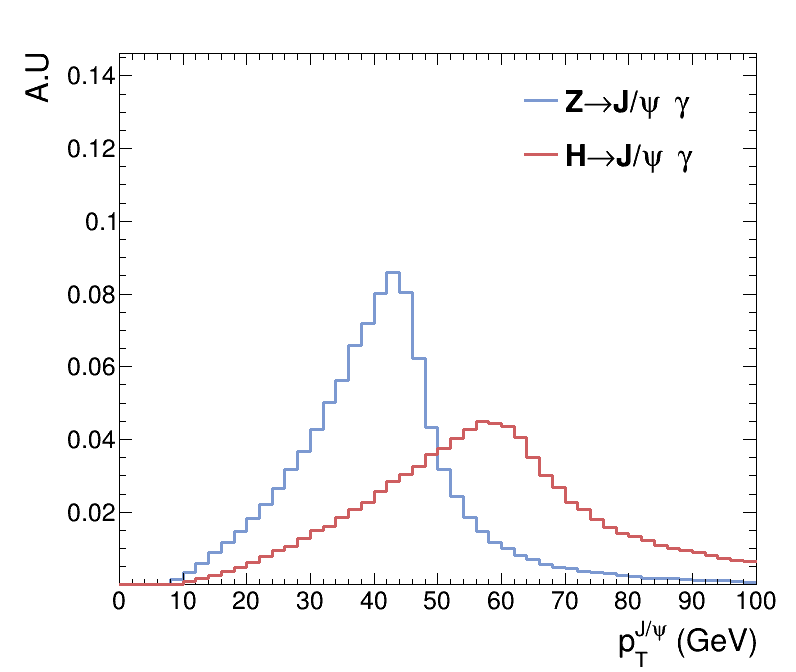
\includegraphics[width=0.33\textwidth]{Fig/GenLevel_HJpsiG/plot_ZHJpsiG/ZHJpsiG_dimuPt}\\
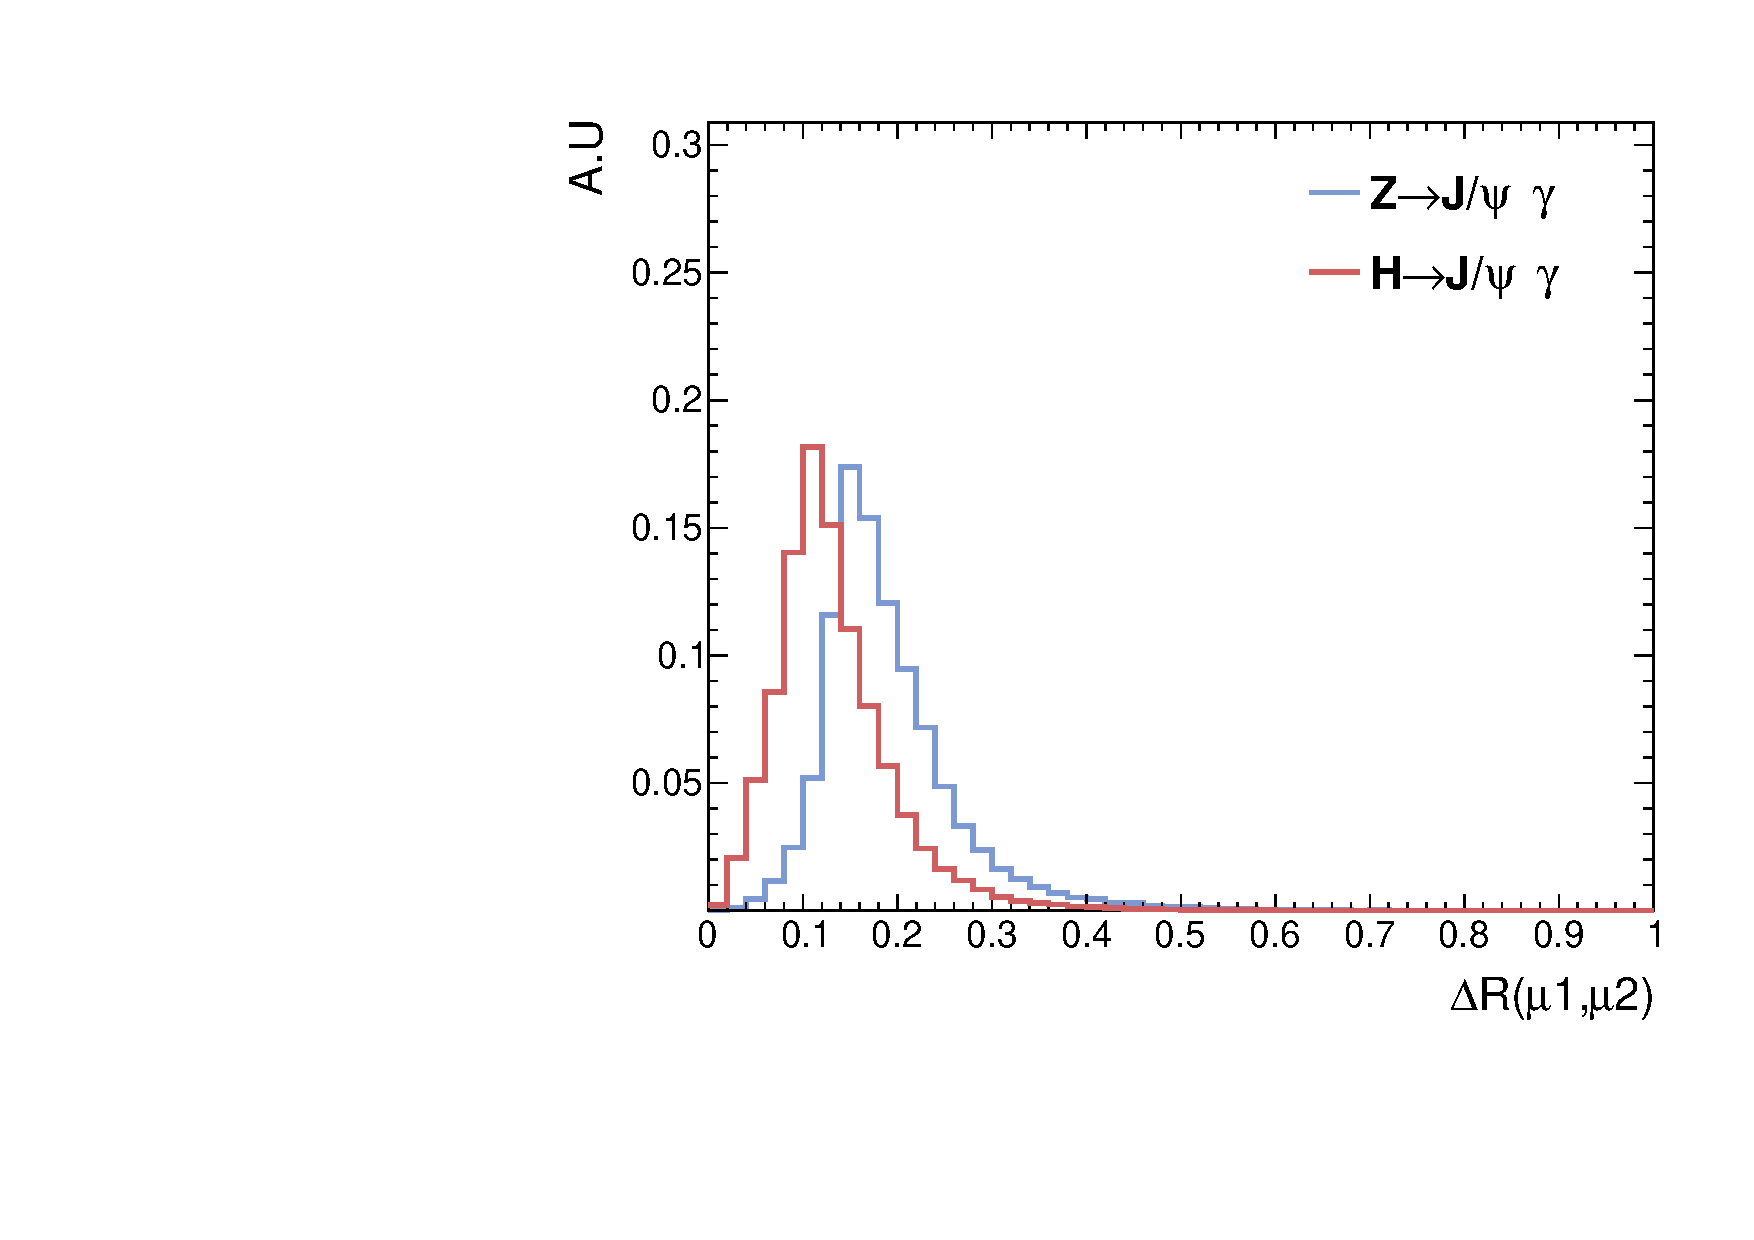
\includegraphics[width=0.33\textwidth]{Fig/GenLevel_HJpsiG/plot_ZHJpsiG/ZHJpsiG_dRdimuon}~
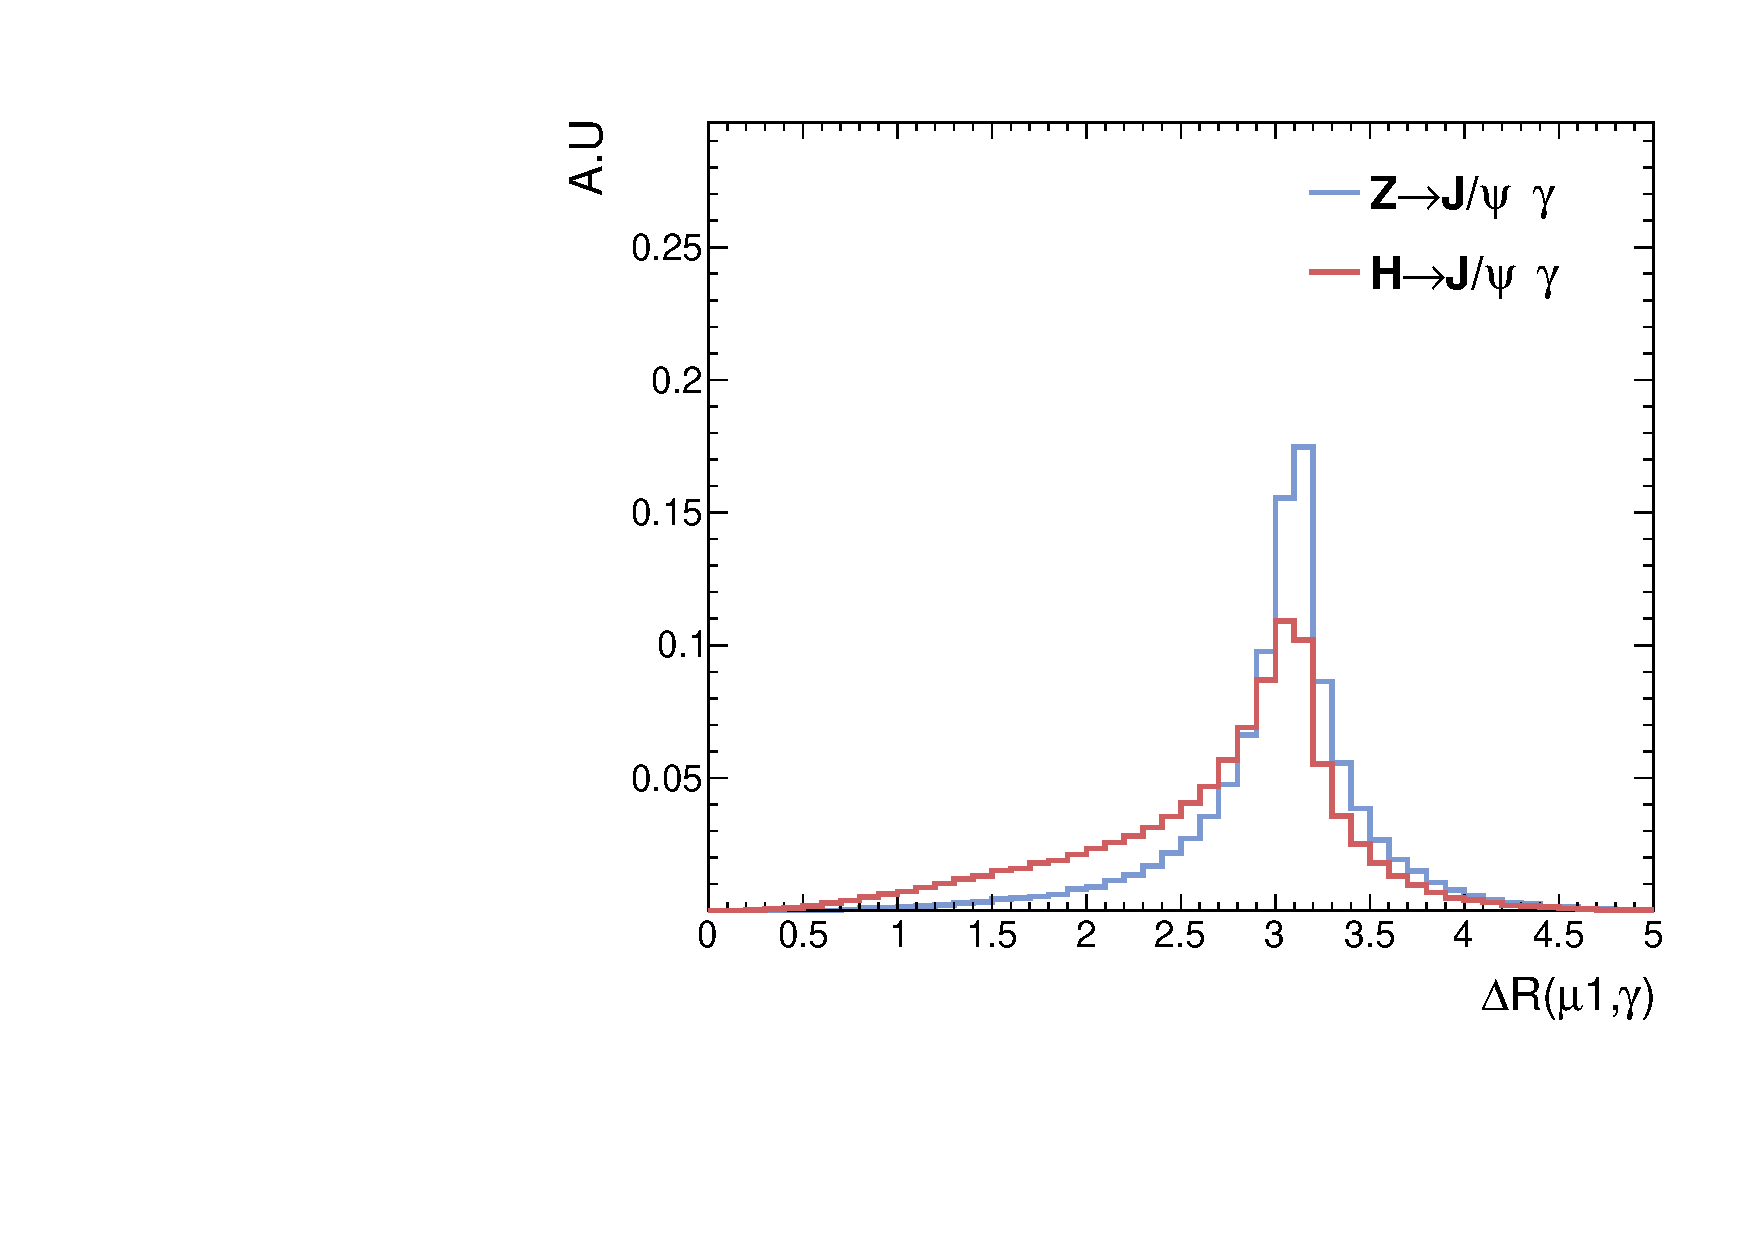
\includegraphics[width=0.33\textwidth]{Fig/GenLevel_HJpsiG/plot_ZHJpsiG/ZHJpsiG_dRmu1pho}~
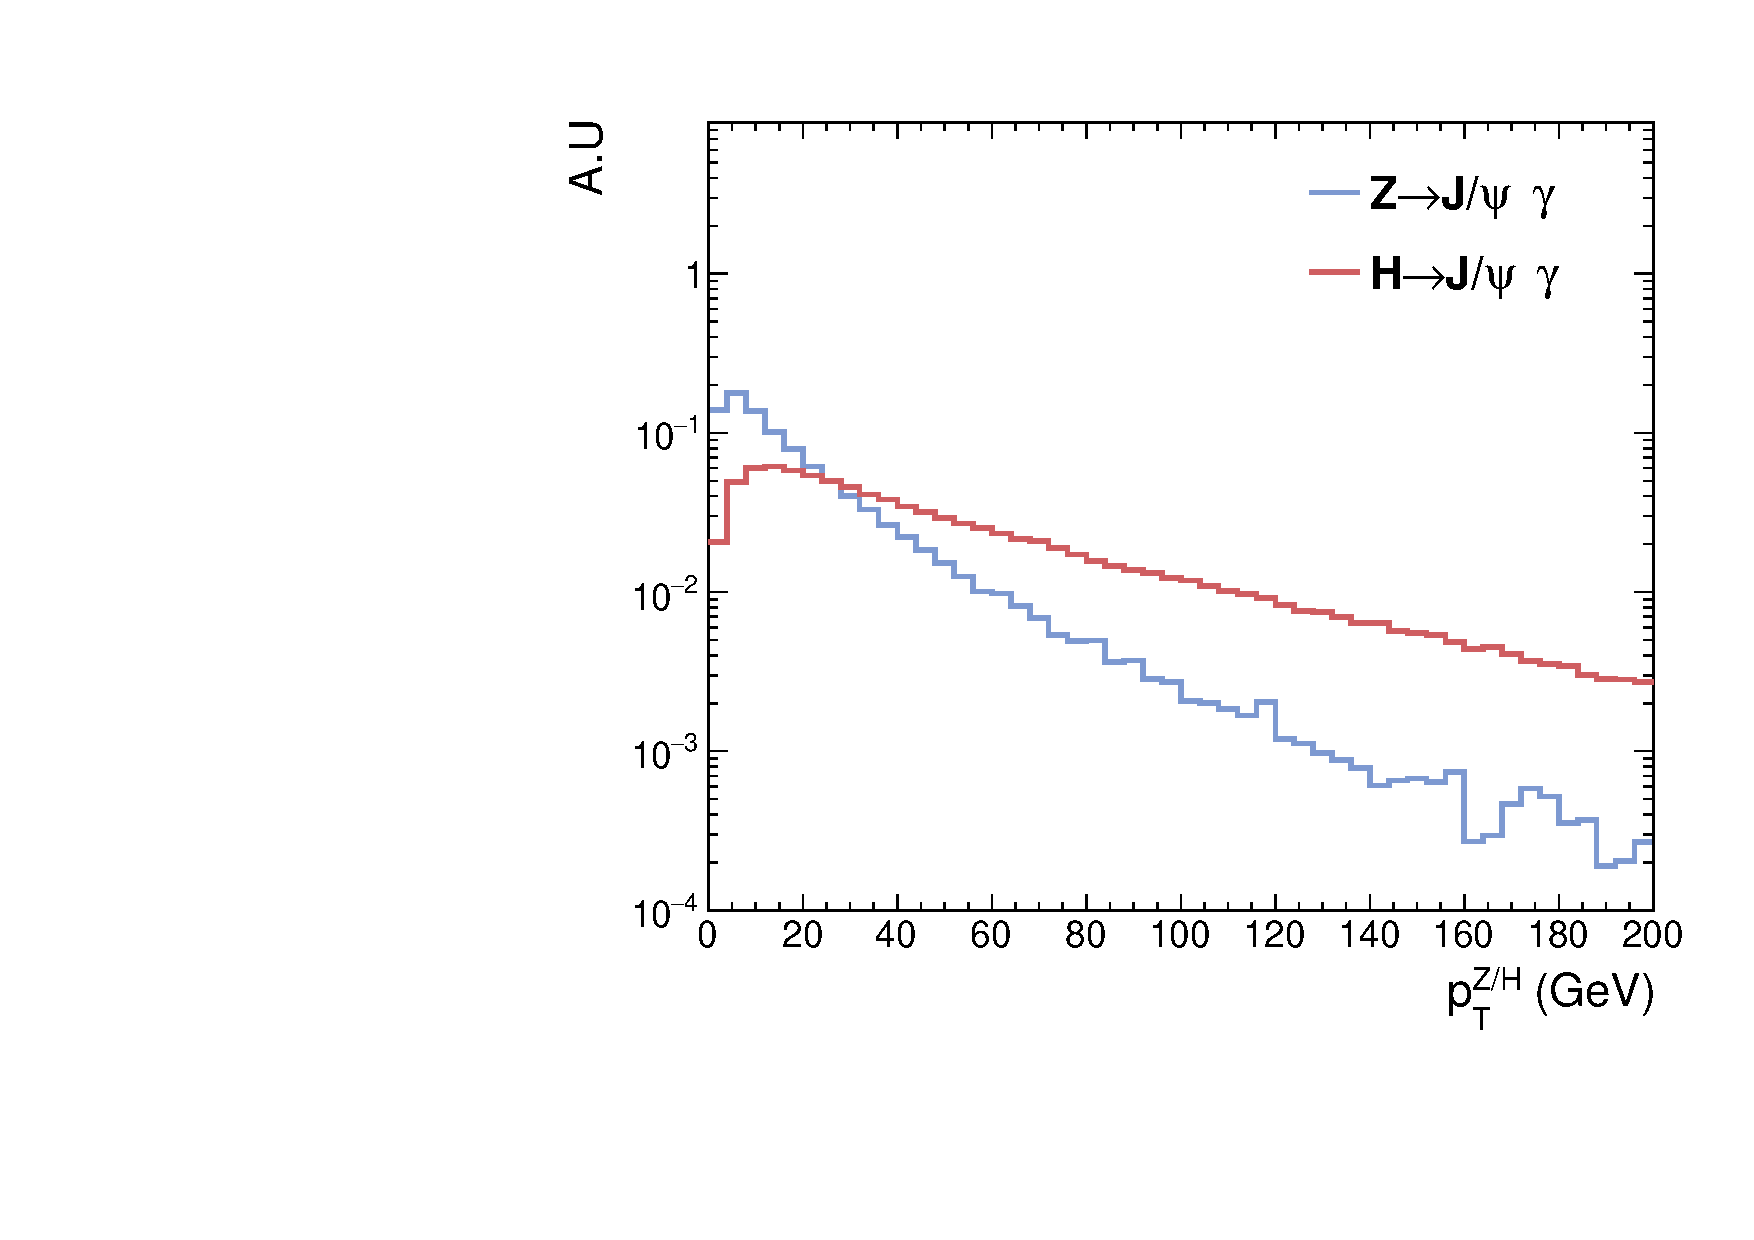
\includegraphics[width=0.33\textwidth]{Fig/GenLevel_HJpsiG/plot_ZHJpsiG/ZHJpsiG_mmgPt}\\
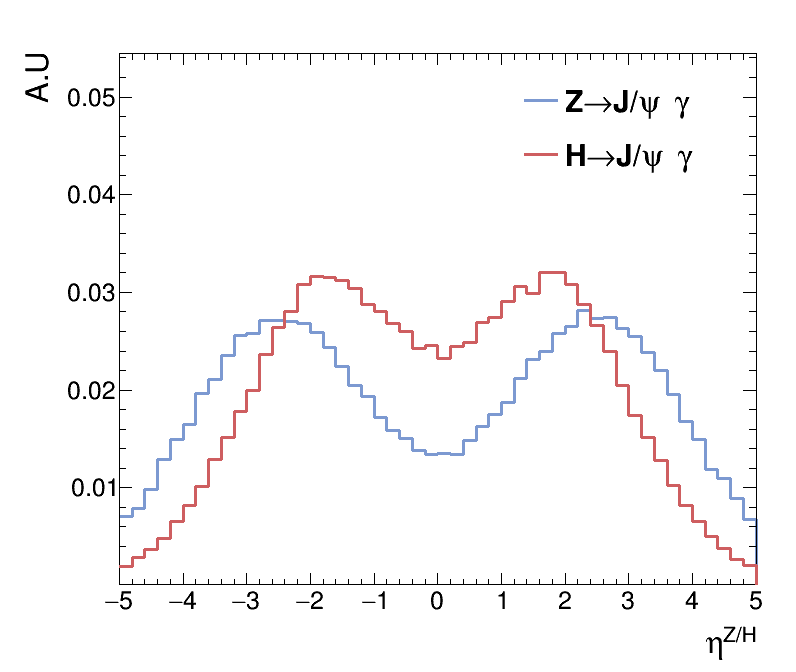
\includegraphics[width=0.33\textwidth]{Fig/GenLevel_HJpsiG/plot_ZHJpsiG/ZHJpsiG_mmgEta}~
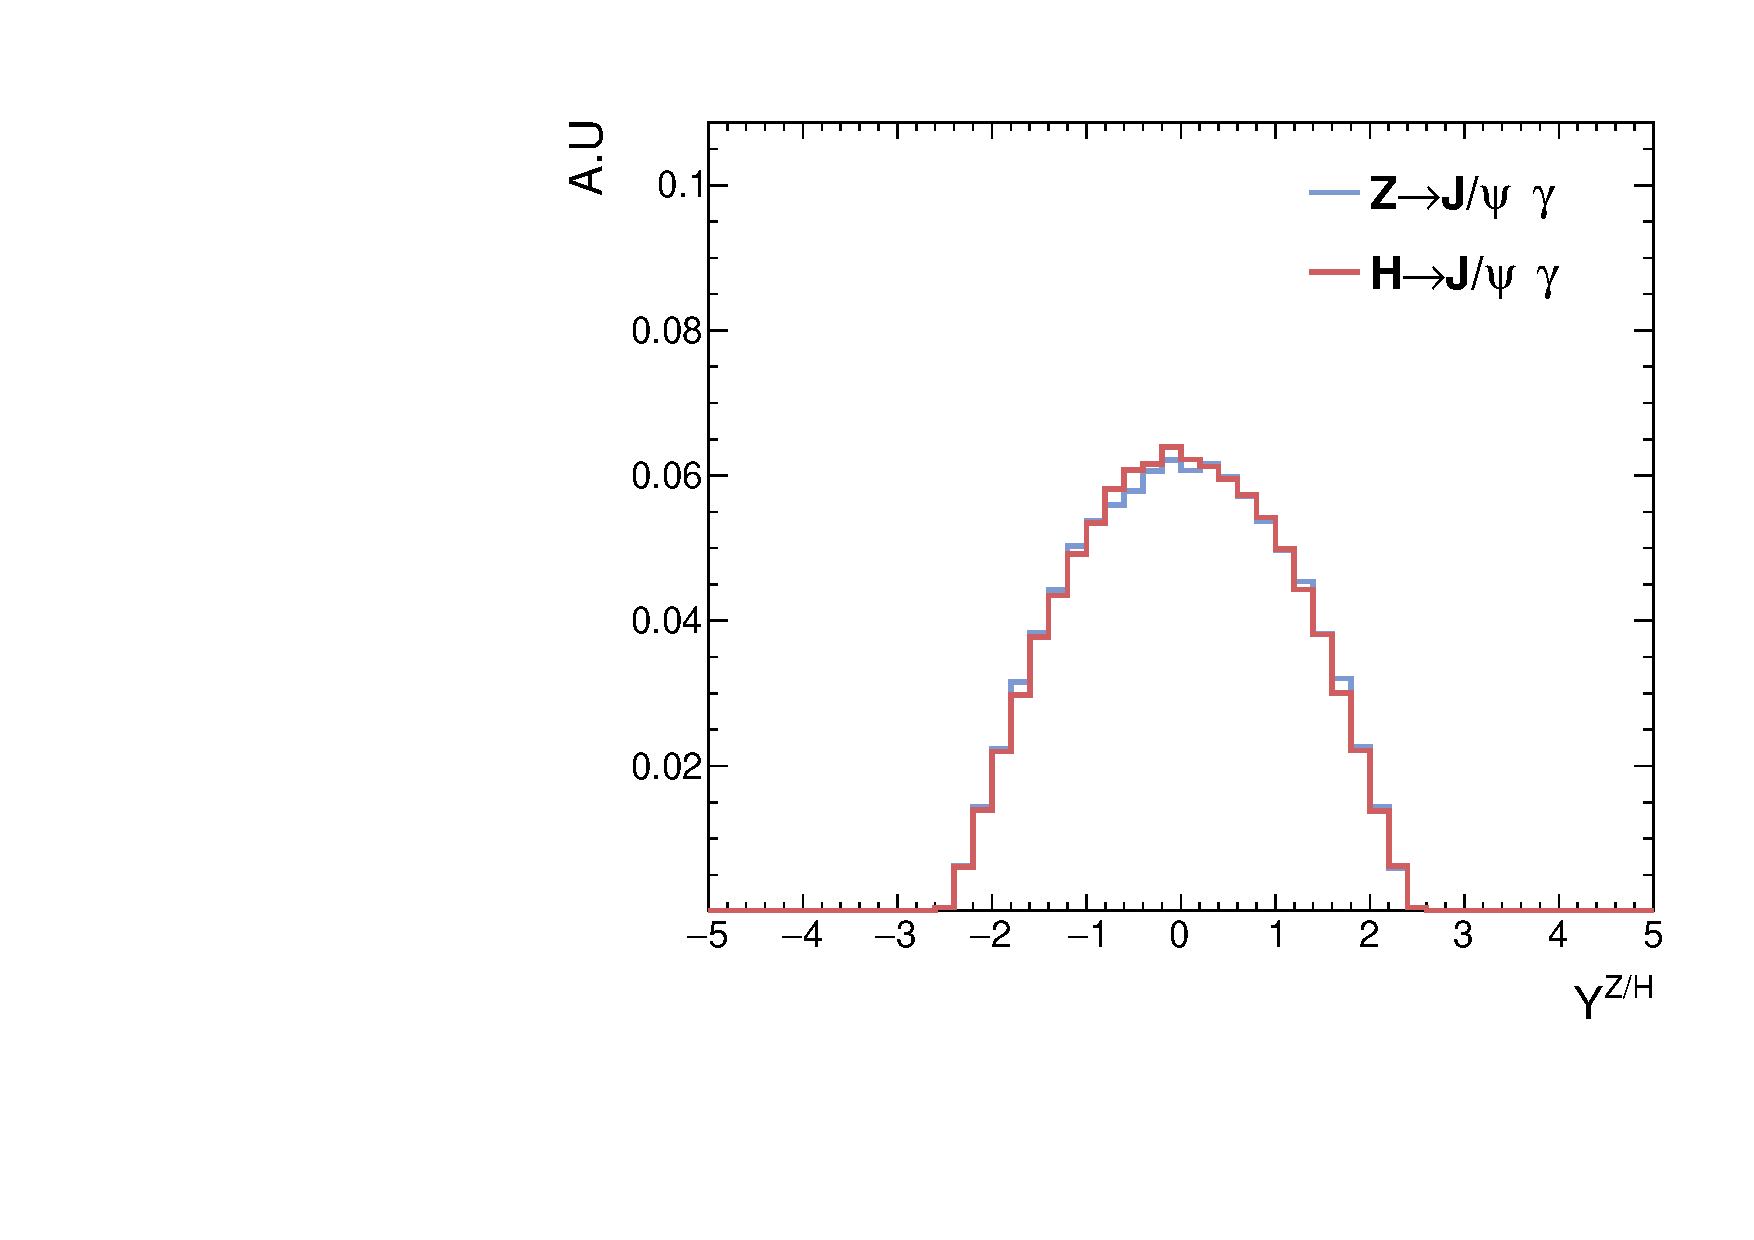
\includegraphics[width=0.33\textwidth]{Fig/GenLevel_HJpsiG/plot_ZHJpsiG/ZHJpsiG_mmgRapidity}\\
\caption{The distributions of key variables at generator level in both the Z and Higgs boson decays: 
	$\pt$ and $\et$ of the leading, trailing muon and the photon,
	pseudorapidity $\eta$ of the leading muon and the photon, $\pt$ of the $\JPsi$ meson , angular separation $\Delta \text{R}$ between muons, $\Delta \text{R}$ between the leading muon and the photon, $\pt$ of the $\cPZ$ and Higgs boson, $\eta$ of the $\cPZ$ and Higgs boson, and the rapidity Y of the $\cPZ$ and Higgs boson}  
\label{fig:GenLevel_HJpsiG}\end{center}\end{figure}  

%\begin{figure}[h]\begin{center}  
%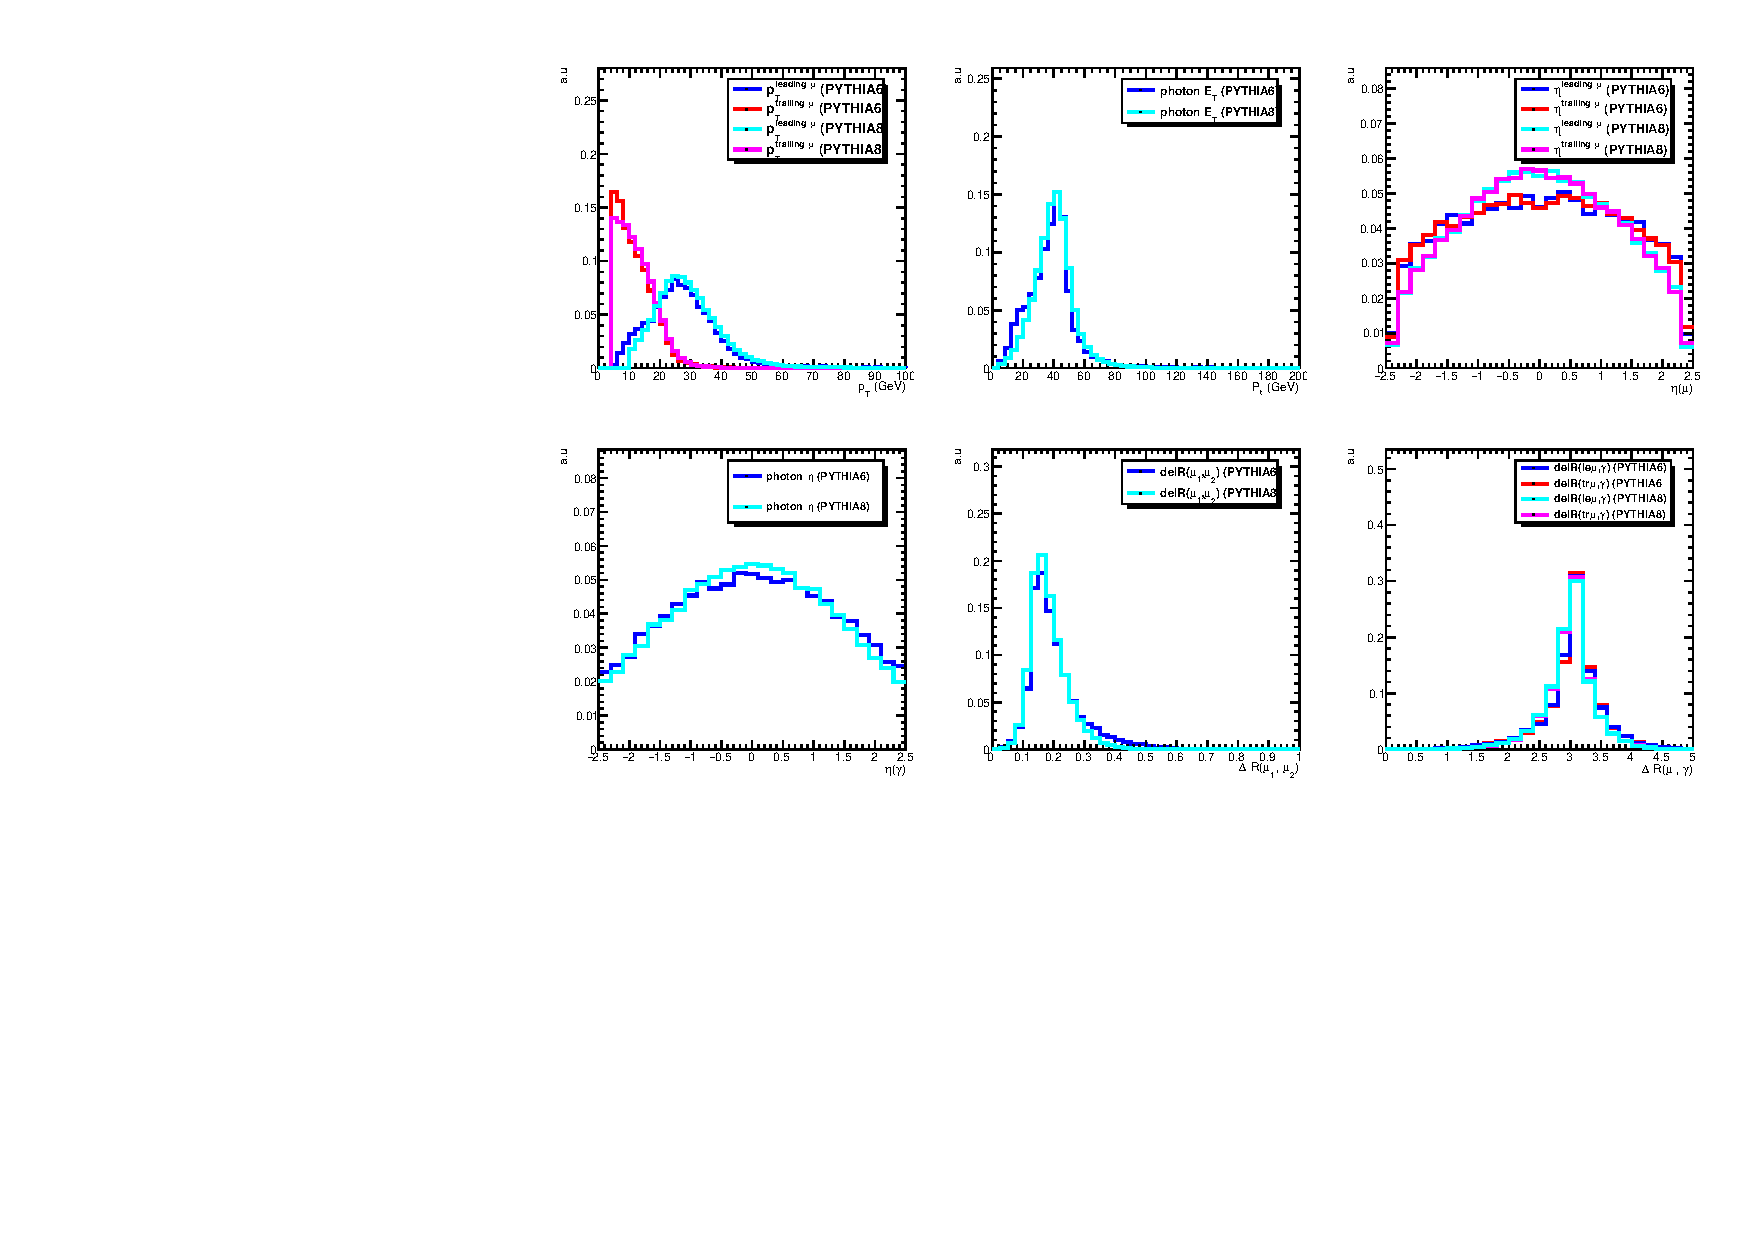
\includegraphics[width=0.95\textwidth]{Fig/GenLevel_ZJpsiG/GenLevelStudy_ZJpsigamma_74XvsSummer16}
%\caption{The kinematic distribution of key variables at generator level in $Z\rightarrow J/\psi + \gamma$ decay: 
%	Transverse momenta of the leading/trailing $\pt$ muon and the photon,
%	pseudorapidity of the muons and the photon, distances $\Delta R_{E_{T}a\phi}$ between the two muons and between the muons and the photon. In this figur%e, two signal samples are compared: one produced by Pythia6 and the other by Pythia8.}  
%\label{fig:GenLevel_ZJpsiG}\end{center}\end{figure}  

%\begin{figure}[!ht]\begin{center}
%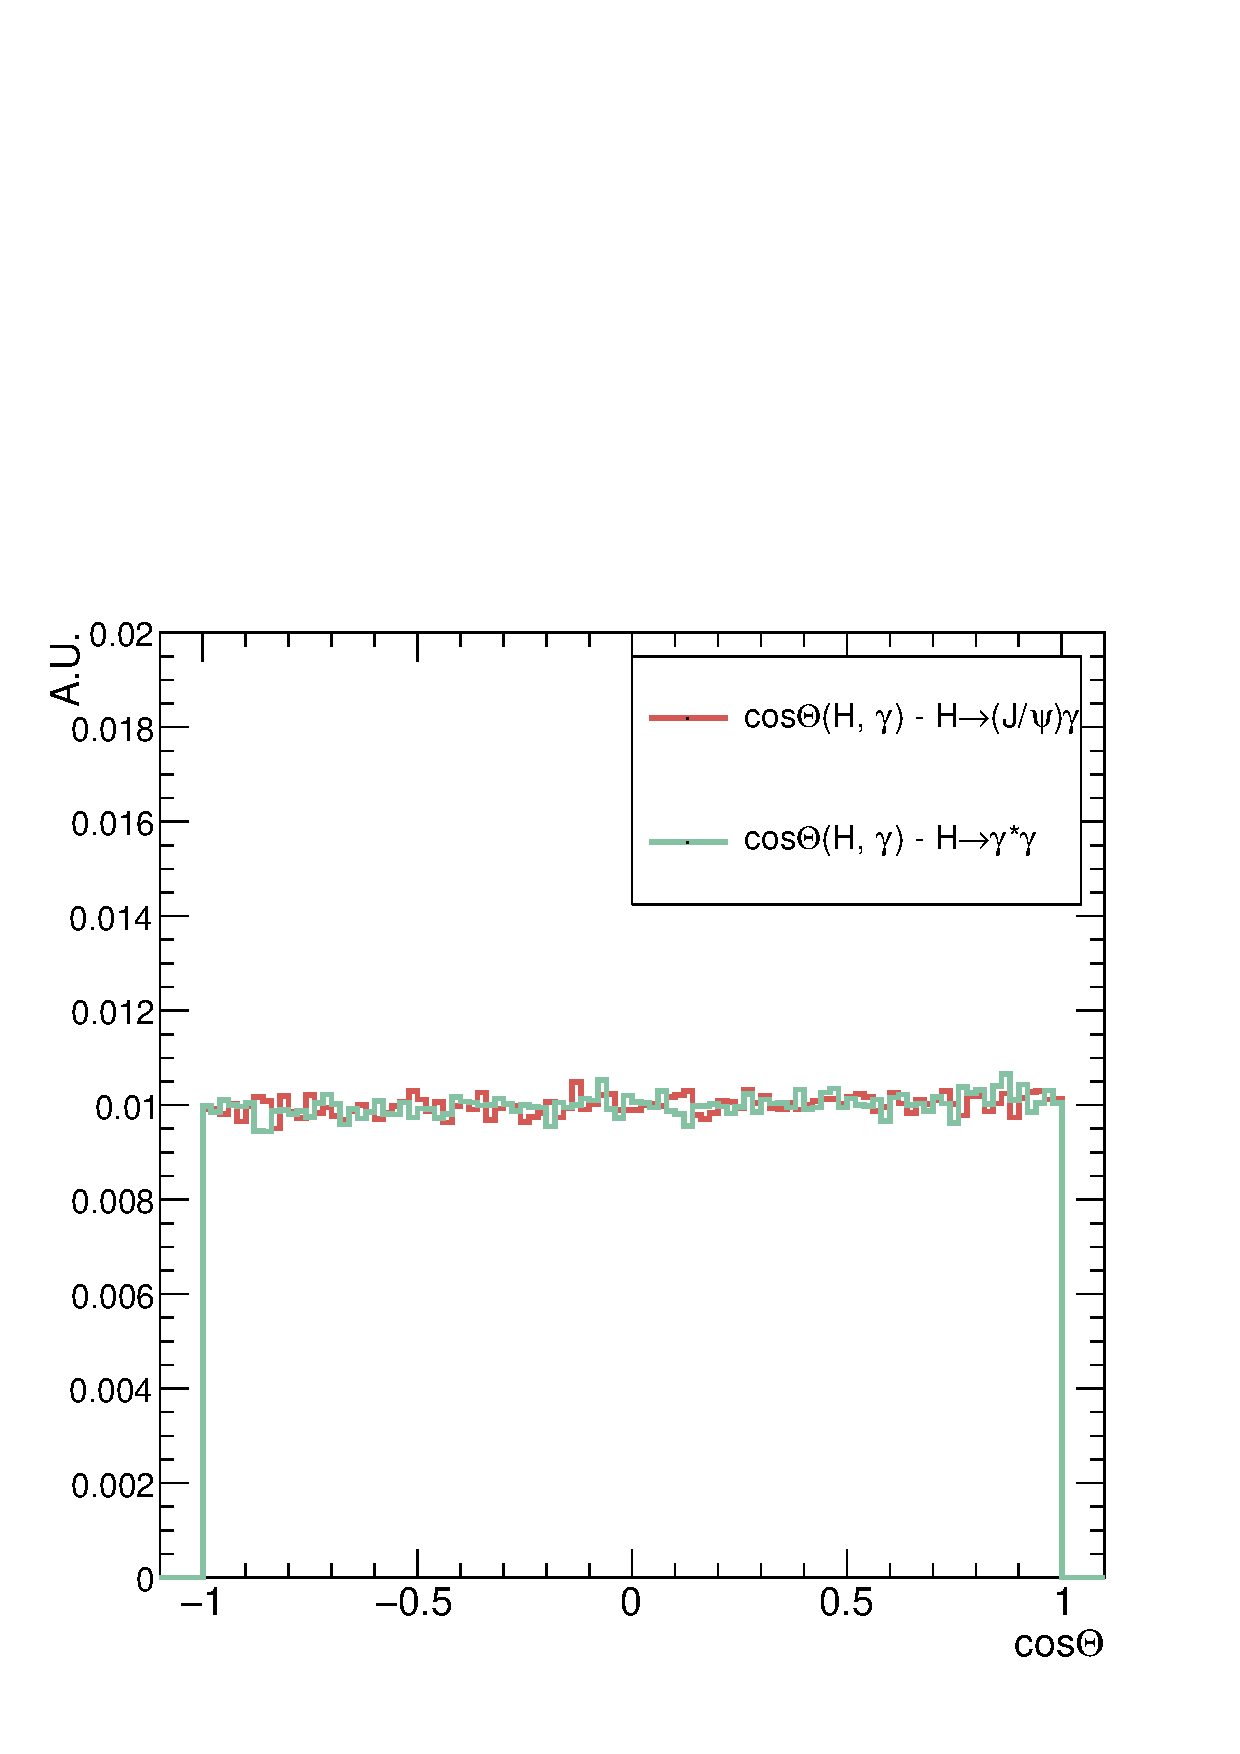
\includegraphics[width=0.7\textwidth]{Fig/GenLevel_HJpsiG/CosTheta_v4}
%\caption{The distribution of $\text{cos}\Theta$, where $\Theta$ is the angle between the direction of the Higgs and the $\gamma$ in the center-of-mass frame of the Higgs. This angle is derived at generator level.}
%\label{fig:CosTheta_H_gamma}\end{center}\end{figure}

\subsection{Previous results from the ATLAS and CMS Collaborations}
The $\cPZ \to\JPsi\ \gamma$ decay was searched for by the ATLAS Collaboration using the data set collected at $\sqrt{s}=8\TeV$~\cite{Aad:2015sda}. An observed (expected) upper limit on the branching fraction of $2.6\ (2.0^{+1.0}_{-0.6})\ten{-6}$ was reported. 
Searches for the $\PH\to\JPsi\ \gamma$ decay have been performed by the ATLAS and CMS Collaborations using the data set collected at $\sqrt{s}=8\TeV$ respectively~\cite{Aad:2015sda,Run1Paper_Dalitz}. Observed (expected) limits on the branching fraction were $1.5\ (1.2^{+0.6}_{-0.3})\ten{-3}$ from the ATLAS Collaboration and $1.5\ (1.6^{+0.8}_{-0.8})\ten{-3}$ from the CMS Collaborations. Fig.~\ref{fig:ATLAS8TeV} shows the three-body invariant mass $m_{\mu\mu\gamma}$ and $\pt^{\mu\mu\gamma}$ distributions, along with the signal-plus-background fit to observed data collected at $\sqrt{s}=8\TeV$ from ATLAS results. Fig.~\ref{fig:CMS8TeV} shows the non-resonant background fit to the $m_{\mu\mu\gamma}$ distributions observed in data collected at $\sqrt{s}=8\TeV$ with CMS search.
Recently, ATLAS provides results with data collected in 2016 for both decays. An observed (expected) upper limit on the branching fraction of $\cPZ \to\JPsi\ \gamma$ decay is set at $2.3\ (1.1^{+0.5}_{-0.3})\ten{-6}$, and of the $\PH\to\JPsi\ \gamma$ is at $3.5\ (3.0^{+1.4}_{-0.8})\ten{-4}$~\cite{Aaboud:2018txb}.
Fig.~\ref{fig:ATLAS2016} shows the recent results from ATLAS Collaboration.
%The ATLAS Collaboration has also searched for the $\PH\to\ccbar$ decay in the $\Pp\Pp \to \cPZ\PH$ production mode using data collected at $\sqrt{s}=13\TeV$~\cite{Aaboud:2018fhh}, and reported observed (expected) limits on $\sigma/\sigma_{\text{SM}}$ ratio of 110 ($150^{+80}_{-40}$), where the $\sigma_{\text{SM}}$ is the expected SM value for the cross section.

\begin{figure}[!ht]
  \begin{center}  
    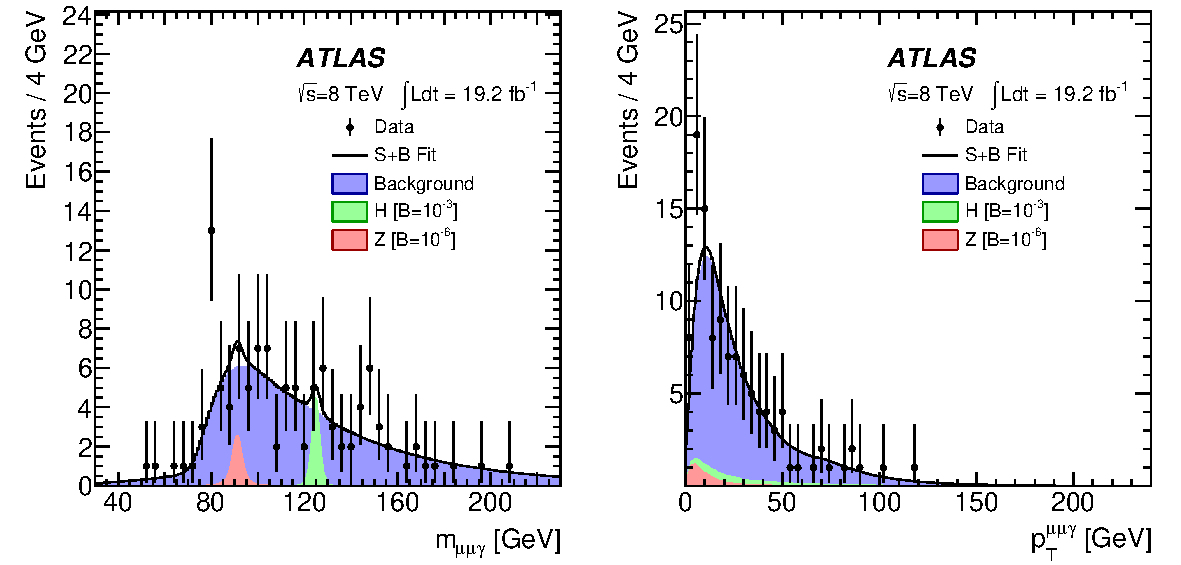
\includegraphics[width=0.99\textwidth]{Fig/PreviousResult/fig_01.pdf}\\
    \caption{Previous result of $\cPZ\ (\PH)\to\JPsi\ \gamma$ decay search from the ATLAS Collaboration. The three-body invariant mass $m_{\mu\mu\gamma}$ and $\pt^{\mu\mu\gamma}$ distributions, along with the results of signal-plus-background fit to observed data collected at $\sqrt{s}=8\TeV$~\cite{Aad:2015sda}.  \label{fig:ATLAS8TeV}}  
  \end{center}
\end{figure}

\begin{figure}[!ht]
  \begin{center}  
    \includegraphics[width=0.7\textwidth]{Fig/PreviousResult/CMS-HIG-14-003_Figure_005.pdf}\\
    \caption{Previous result of $\PH\to\JPsi\ \gamma$ decay search from the CMS Collaboration. Non-resonant background fit to the $m_{\mu\mu\gamma}$ distributions observed in data collected at $\sqrt{s}=8\TeV$~\cite{Aad:2015sda}.}  
    \label{fig:CMS8TeV}
  \end{center}
\end{figure}

\begin{figure}[!ht]
  \begin{center}  
    \includegraphics[width=0.99\textwidth]{Fig/fig_04a_ATLAS2016}\\
    \caption{Result of $\cPZ\ (\PH)\to\JPsi\ \gamma$ decay search from the ATLAS Collaboration with data collected at $\sqrt{s}=13\TeV$ in 2016~\cite{Aaboud:2018txb}.\label{fig:ATLAS2016}}  
  \end{center}
\end{figure}
%\begin{figure}[!ht]
%  \begin{center}  
%    \includegraphics[width=0.45\textwidth]{Fig/PreviousResult/fig_02a}~
%    \includegraphics[width=0.45\textwidth]{Fig/PreviousResult/fig_02b}\\
%    \caption{Result of $\PH\to\ccbar$ search in the $\Pp\Pp\to\cPZ\PH$ production mode using data collected at $\sqrt{s}=13\TeV$ from the ATLAS Collaboration.}  
%    \label{fig:ATLASHcc}
%  \end{center}
%\end{figure}
	\chapter{Experimental apparatus}
\label{Chap:CMS}
In this chapter, the overview of the Large Hadron Collider (LHC) and the Compact Muon Solenoid (CMS) will be introduced. The object reconstruction will be summarized in the last section, as it is closely related to the detectors. 

\section{Large Hadron Collider}
The LHC is so far the largest particle accelerator that human have ever built, and currently hosted by the Europe Organization of Nuclear Research (CERN). 
It possesses a 26.7~km of ring and is placed more than 100~m deep beneath Geneva and France. Such large circumference makes it able to provide high energy collisions, and enables us to examine the validity of the SM and explore the physics such as the existence of the Higgs boson, supersymmetry particles (SUSY), extra-dimension, or even dark matter (DM). The ring consists of two individual and parallel beam pipes, in which protons (or heavy-ions) circulate in opposite directions. 

The protons are grouped together into 2808 bunches, and each bunch contains $1.15\ten{11}$ protons. The time interval between two bunches is 25\unit{ns}, corresponding to a collision rate of 40\unit{MHz}.
A series of machines then successively accelerate and bring proton beams to higher energy. Each beam is accelerated up to an energy of 6.5\TeV when it finally arrives at the LHC beam line. 
%The history of proton beams in the pre-acceleration stage is briefly described below: 
%\begin{itemize}
%\item Protons are obtained by stripping the electrons off the hydrogen atoms which are taken from the hydrogen contained in a bottle.
%\item Protons are injected to the Linear Accelerator (LINAC2) and accelerated to an energy of 50\MeV. 
%\item The Proton Synchrotron Booster (PSB) accelerates the protons from the LINAC2 to 1.4\GeV. 
%\item The PSB feeds the protons to the Proton Synchrotron (PS), where the protons are accelerated to 25\GeV. 
%\item The energy of the protons is brought up to 450\GeV by the Super Proton Synchrotron (SPS). The protons will then be split into two beams, one in a clockwise and the other in an anticlockwise direction, and transferred to the LHC. 
%\item In the LHC beam line, the beams are both accelerated to 6.5\TeV. 
%\end{itemize}

\begin{figure}[!ht]
  \begin{center}
    \includegraphics[width=0.95\textwidth]{Fig/Cern_Complex}\\
    \caption{The CERN accelerator complex. The protons are accelerated from the LINAC2, PSB, PS, SPS, and finally to LHC~\cite{Mobs:2197559}.}
    \label{fig:cerncomp}
  \end{center}
\end{figure}

Fig.~\ref{fig:cerncomp} shows the whole system of the CERN complex~\cite{Mobs:2197559}. 
%There are four intersections where experiments are located, as shown in four yellow points in Fig.~\ref{fig:cerncomp}. Particle beams are focused by quadrapole magnets to collide here. \textbf{A Toroidal LHC Apparatus (ATLAS)} and \textbf{Compact Muon Solenoid (CMS)} are two general purpose detector aiming at looking for the Higgs boson, searching for any possible signature of new physics, and probing the physics in the \TeV scale. These two experiments are complementary on extending the physical reach and providing the mutual evidence of findings. \textbf{LHC-beauty (LHCb)} is a specialized detector for b-physics (``b'' stands for bottom, or beauty, quarks), for which scientists believe that by measuring the properties of charge-conjugate and parity (CP) in decays of these heavy-flavor particles, it may reveal some useful clues as to the matter-antimatter asymmetry in our universe.  \textbf{A Large Ion Collider Experiment (ALICE)} is dedicated to heavy-ion physics (such as lead-lead collisions, or the xenon-xenon collisions that recently performed). The quark–gluon plasma can be produced in heavy-ion collisions, and its properties are key ingredients to understand the origin of color confinement in quantum chromodynamics (QCD). 

An important quantity in the collider physics is the luminosity $\Lumi$. The instantaneous luminosity is defined as:
\begin{equation}
	\frac{\mathrm d N}{\mathrm d t}=\sigma_{\text{event}}\frac{\mathrm d \Lumi}{\mathrm d t}
\end{equation}
The $\frac{\mathrm d N}{\mathrm d t}$ is the event production rate, and $\sigma_{\text{event}}$ is the interaction cross section.
The integrated luminosity $\Lumi_{\text{Tot}}$ is the integral of the instantaneous luminosity over a period of time. The $\Lumi_{\text{Tot}}$ is a measure of the amount of data. Fig.~\ref{fig:IntegratedLumi} shows the integrated luminosity that CMS recorded in each data-taking year~\cite{CMSLUMI}. 

\begin{figure}[!ht]
  \begin{center}
    \includegraphics[width=0.95\textwidth]{Fig/int_lumi_cumulative_pp_2}\\
    \caption{Cumulative luminosity versus day delivered to CMS during stable beams for pp collisions at nominal center-of-mass energy. This is shown for data-taking in 2010 (green), 2011 (red), 2012 (blue), 2015 (purple), 2016 (orange), 2017 (light blue), and 2018 (deep blue)~\cite{CMSLUMI}. \label{fig:IntegratedLumi}}
  \end{center}
\end{figure}

\section{Compact Muon Solenoid}
Compact Muon Solenoid is one of the general purpose detectors located at the LHC ring. 
%A detailed description of the CMS detector, together with a definition of the coordinate system used and the relevant kinematic variables, can be found in~\cite{CMS-Jinst}.
The central feature of the CMS apparatus is a superconducting solenoid of 13\unit{m} in length and 6\unit{m} in internal diameter, providing an axial magnetic field of 3.8\unit{T}. Within the solenoid volume are a silicon pixel and strip tracker, a lead tungstate crystal electromagnetic calorimeter (ECAL), and a brass and scintillator hadron calorimeter (HCAL), each composed of a barrel and two endcap sections. Forward calorimeters extend the pseudorapidity ($\eta$) coverage provided by the barrel and endcap detectors. Muons are detected in gas-ionization chambers embedded in the steel flux-return yoke outside the solenoid. 

The adopted coordinate system, as shown in Fig.~\ref{fig:cmscoordinate} has the origin at the nominal collision point inside CMS detector, where the y-axis pointing vertically upward, the x-axis pointing radially inward toward the center of the LHC, and the z-axis pointing along the beam direction. The azimuthal angle $\phi$ is measured from the x-axis in the x-y plane, while the polar angle $\theta$ is measured from the z-axis. 
Rapidity, $\mathit{Y}$, is defined as $\mathit{Y}\equiv\frac{1}{2}\ln\big(\frac{E+p_{z}c}{E-p_{z}c}\big)$, where $E$ is the energy of the particle and $p_{z}$ is the momentum in the z direction.
This Lorentz invariant quantity indicates the angle between the x-y plane and the direction of the measured particle.
For the highly relativistic particles, the other quantity called pseudorapidity, defined as $\eta = -\ln \tan(\theta /2)$, is used, where $\theta$ is the angle between the particle trajectory and the z-axis (beam pipe).

\begin{figure}[!ht]
  \begin{center}
    \includegraphics[width=1.0\textwidth]{Fig/cms_coordinate}\\
    \caption{The adopted coordinate system in CMS. \label{fig:cmscoordinate}}
  \end{center}
\end{figure}

The momentum and energy transverse to the beam direction, denoted by $\pt$ and $\et$ , respectively, are computed from the x and y components.

\begin{figure}[!ht]
  \begin{center}
    \includegraphics[width=0.85\textwidth]{Fig/cms_120918_03}\\
    \caption{A cutaway view of the CMS detector~\cite{Sakuma:1626816}. \label{fig:CMSdetector}}
  \end{center}
\end{figure}
Fig.~\ref{fig:CMSdetector} shows a global view of the CMS detector~\cite{Sakuma:1626816}. Brief description of each sub-detector is summarized as follows.

\subsection*{Superconduction magnet}
The superconducting solenoid magnet, formed by a cylindrical coil of superconducting fibers, was originally designed to provide a magnetic field of 4 Tesla (T), while in the actual operation it produces a 3.8\unit{T} of field. Such large bending power enables us to measure the momentum of high energy charged particles precisely. 
The magnetic field is confined to the volume of the detector. This is done by the steel yoke, consisting five layers for barrel part and three layers for each endcap. 
\subsection*{Silicon tracker}
The CMS tracker is composed of two systems: a pixel detector (for a total of 1440 silicon pixel modules) with three barrel layers, and a silicon strip tracker (for a total of 15148 silicon strip modules) with ten barrel detection layers, four layers of tracker inner barrel (TIB) and six layers of tracker outer barrel (TOB), extending outwards. 
Each system is completed by endcaps, which consist of two disks in the pixel detector, three tracker inner disks (TID) and nine disks of tracker endcaps (TEC) in the strip tracker on each side of the barrel. The acceptance of the whole tracker system extends up to a $|\eta|<2.5$. 
Fig.~\ref{fig:TrkerLayout} shows the schematic view of the silicon tracker in the r-z plane. The upper plot is the cross section through the tracker, and the lower one is one quarter of the tracker, where the paths of the laser rays (R), the alignment tubes (A) and the beam splitters (B) of the laser alignment system are illustrated.

For non-isolated particles with transverse momentum, $\pt$, between 1 and 10GeV and $|\eta|<1.4$, the track resolutions are typically 1.5\% in $\pt$ and 25–90 (45–150) $\mu$m in the transverse (longitudinal) impact parameter~\cite{TRK-11-001}.

\begin{figure}[!ht]
  \begin{center}
  \includegraphics[width=0.7\textwidth]{Fig/CMS_Detector/TrakerLayout}\\
    \includegraphics[width=0.6\textwidth]{Fig/CMS_Detector/figs_TrackerLayoutWithLAS}\\
    \caption{Schematic view of one quarter of the silicon tracker in the r-z plane~\cite{Chatrchyan:2008aa}.\label{fig:TrkerLayout}}
  \end{center}
\end{figure}

\subsection*{Electromagnetic calorimeter}
The electromagnetic calorimeter (ECAL) is a homogeneous calorimeter made of 61200 lead tungstate ($\text{PbWO}_{4}$) crystals in the barrel part ($0<|\eta|<1.48$) and 7324 crystals in each of endcaps ($1.48<|\eta|<3.0$). 
The high density ($8.28\unit{g}/\unit{cm}^{3}$) and short radiation length $\text{X}_{0}$\footnotemark ($0.89\unit{cm}$) of the crystal result in a compact calorimeter with fast response, fine granularity, and strong resistance to the radiation. A sampling calorimeter, preshower detector (ES), is placed in front of the endcap crystals and covers the range of $1.65<|\eta|<2.6$.  It consists of two planes of silicon sensors interleaved with a total of 3$\text{X}_{0}$ of lead.
The main task of this detector is to help on distinguishing between single high-energy photons and the close pairs of low-energy photons, usually from the decay of neutral pion. The ES also improves the ability of identifying electrons against minimum ionizing particles and the position determination of electrons and photons . Fig.~\ref{fig:EcalLayout} shows layout of the CMS ECAL.
\footnotetext{One radiation length of a given material is defined as the distance after which the electron loose $1/\mathrm{e}$ of its original energy.}
\begin{figure}[!ht]
  \begin{center}
 	%\includegraphics[width=0.75\textwidth]{Fig/CMS_Detector/ECAL_layout}\\
  	\includegraphics[width=0.7\textwidth]{Fig/CMS_Detector/Figure_004-001}\\
    \caption{Layout of the ECAL~\cite{Benaglia:2014aqa}.}
    \label{fig:EcalLayout}
  \end{center}
\end{figure}

\subsection*{Hadron calorimeter}
The hadron calorimeters (HCAL), a sampling calorimeter, measures the energy of hadron jets and provides indirect measurement of missing transverse energy, which can be neutrinos or exotic particles that do not interact with matters.  
Fig.~\ref{fig:HCalLayout} shows the longitudinal view of the CMS detector with the dashed lines representing fixed $\eta$ values. 
The HCAL consists four parts: the HCAL barrel (HB), the HCAL endcap (HE), the HCAL outer (HO), and the HCAL forward (HF). 
The HB, covering the range of $|\eta|<1.3$, is placed radially between the outer extent of the ECAL and the inner extent of the magnet coil. The HO sits outside the solenoid complementing the barrel part, and ensure the leakage of the energy not detected by HB to be minimal.
The HE covers the range of $1.3<|\eta|<3.0$, a region containing about 34\% of the particles produced in the final state.
The HF is place at the range of $|\eta|>3.0$, where much higher energy will be deposited compared to other sub-detectors.  
\begin{figure}[!ht]
  \begin{center}
  \includegraphics[width=0.7\textwidth]{Fig/CMS_Detector/HCAL_layout}\\
    \caption{Longitudinal view of the CMS detector showing the locations of the hadron barrel (HB), endcap (HE), outer (HO) and forward (HF) calorimeters~\cite{Chatrchyan:2008aa}. \label{fig:HCalLayout}}
  \end{center}
\end{figure}

\subsection*{Muon system}
The muon system is located outside the solenoid and covers the range $|\eta|<2.4$. It is composed of three types of gaseous detectors, drift tubes (DTs), cathode strip chambers (CSCs), and resistive plate chambers (RPCs), sandwiched among the layers of the steel yoke. 
The DTs are segmented into drift cells; the position of the muon is determined by measuring the drift time to an anode wire of a cell with a shaped electric field. 
The CSCs operate as standard multi-wire proportional counters but with a finely segmented cathode strip readout, which yields an accurate measurement of the position of the bending plane $(\text{R}-\phi)$ coordinate at which the muon crosses the gas volume. 
The DT and CSC chambers are located in the regions $|\eta| < 1.2$ and $0.9 < |\eta| < 2.4$, respectively, and are complemented by RPCs in the range $|\eta| < 1.9$. Three regions are defined and referred to as the barrel ($|\eta| < 0.9$), overlap ($0.9 < |\eta| < 1.2$), and endcap ($1.2 < |\eta| < 2.4$) regions~\cite{Sirunyan:2018fpa}. 
Fig.~\ref{fig:MuonSystLayout} shows the arrangement of the muon system. 
\begin{figure}[!ht]
  \begin{center}
  \includegraphics[width=0.7\textwidth]{Fig/CMS_Detector/MuonSystem_layout}
    \caption{An R-z cross section of the muon station. The drift tube stations (DTs) are labeled MB ("Muon Barrel'') and the cathode strip chambers (CSCs) are labeled ME ("Muon Endcap''). Resistive plate chambers (RPCs) are mounted in both the barrel and endcaps of CMS, where they are labeled RB and RE, respectively~\cite{Sirunyan:2018fpa}. \label{fig:MuonSystLayout}}
  \end{center}
\end{figure}

\subsection*{Trigger and data acquisition system}
The LHC provides $\Pp\Pp$ and heavy-ion collisions at high interaction rate. This corresponds to an enormous amount of data that are currently not able to be completely stored. Furthermore, most of these interactions would be low-energy glancing collisions, rather than energetic and head-on interactions where processes of interested may occur. The trigger system is designed to reduce the rate and to start the physics event selection process. Fig.~\ref{fig:TrigSyst} shows the schematic diagram of the trigger architecture and data acquisition system. The level-1 trigger (L1) consists of custom-designed and programmable electronics. Information from muon system (including DTs, CSCs, and RPCs), ECAL, HCAL, and HF is used to reconstruct candidate trigger objects, and these quantities are combined and forwarded to the Global Trigger (GT), which calculates the trigger decision and sends out the signal if it is ''L1 Accept (L1S)``. This step reduces the data rate from the 40 \unit{MHz} of the LHC bunch crossing rate down to a maximum of 100 \unit{kHz}. 
In case of a positive L1 decision all data for the corresponding bunch crossing time is read out from the CMS detector and transferred to the HLT, which consists of a software system implemented in a filter farm. The high level trigger algorithm (HLT) performs a full reconstruction of events using a faster version of offline software and writes data out to permanent storage at a typical rate of several hundred \unit{Hz}.
\begin{figure}[!ht]
  \begin{center}
  \includegraphics[width=0.8\textwidth]{Fig/CMS_Detector/Trigger_architexture}
    \caption{A schematic diagram of the trigger system~\cite{Chatrchyan:2008aa}. \label{fig:TrigSyst}}
  \end{center}
\end{figure}

\section{Object reconstruction}
	\subsection{Particle-Flow algorithm}
%		The PF algorithm event reconstruction was originally developed and used in the ALEPH (Apparatus for LEP PHysics) experiment at LEP, which collided electron and positron beams. 
		The core concept of this algorithm is to optimally correlate tracks or clusters from all sub-detectors and combines the information to reconstruct final state particles. In order to have PF algorithm as efficient as possible, the magnetic field should be strong enough to maximize the separation between charged and neutral particles, and the detector should have fine spatial granularity layers that can distinguish merged particles, especially those in jets. The CMS meets all of these advantages to use PF reconstruction as a global event description. 
%		However, the remnant of the collisions, additional pile-up interactions, the proximity of particles inside an energetic jet, and the interactions in the detector materials dramatically increase the multiplicity and complexity of the final state particles in $\Pp\Pp$ or heavy-ion collisions, and may spoil the quality of the PF reconstruction. Dedicated simulation and commissioning of the data collected during the first few weeks of $\sqrt{s}=7\TeV$ collisions were done, and showed that the performance was not severely degraded. The robustness of the PF algorithm was then widely demonstrated and validated, the usage was therefore confirmed. 

		The ECAL energy clusters without being associated to extrapolated tracks from tracker are reconstructed as photons. Electrons are reconstructed by tracks in the tracker system with associated energy deposits in the ECAL. The bremsstrahlung emission and energy losses when traveling through tracker materials are properly accounted for. Muons tracks can be reconstructed in tracker, in muon system, or the combination of the two. Charged hadrons are reconstructed by the tracks not identified as electrons or muons with energy cluster in HCAL. The energy clusters that correspond to excesses of energy with respect to charged hadrons and not linked to charged particle trajectories are reconstructed as neutral hadrons. 

		In this analysis, photon and muons are selected as final states particles. Hence, their reconstructions are described in detail in the following paragraphs.

\subsection*{Photon reconstruction}
		Photons are reconstructed from energy deposits in the ECAL. The algorithms, without any hypothesis as to whether the particle from the interaction point is a photon or an electron, identify the energy clusters and constrains them to the expected sizes and shapes, based on the study of simulation. The measurements of photon trigger, reconstruction, and identification efficiencies and energy scale and resolution can therefore utilize the electrons from $\cPZ\to e^{+}e^{-}$ events with a well defined invariant mass. 
		
		The clustering algorithms are used to sum over all energy deposits in crystals in the same electromagnetic shower. A basic cluster (BC) is chosen to be the local maximum among the energy deposits. Several BCs are combined to construct a supercluster (SC). The radiated energies, such as the conversions of photons or bremsstrahlung from electrons, are corrected and recovered for their corresponding SC.
		The energy of the photon is determined by summing the amplitude in channels $\mathit{A_{i}}$ over the crystals $i$ in the supercluster where the photon leaves energy, corrected by the intercalibration $\mathit{c_{i}}$ and light monitoring $\mathit{S_{i}(t)}$ constants. The procedure can be summarized in a formula,
		\begin{equation}
		\mathit{E_{\gamma}} = \bigg[ \sum_{i} \bigg(\mathit{S_{i}(t)} \times \mathit{c_{i}} \times \mathit{A_{i}}\bigg) \times \mathit{G}(\eta) + \mathit{E_{ES}} \bigg] \times \mathit{F_{\gamma}}
		\end{equation}
	where $\mathit{G}(\eta)$ is the ADC to \GeV factor. 
		
		Independent methods are used to calculate the intercalibration constants (ICs), and the combined factor is obtained from the mean of the individual IC at a fixed value of $\eta$, weighted by their respective precisions. A light monitoring system, consisting of a system of lasers that inject light to crystals, is used to monitor the time dependence of response in the ECAL resulting from the decreases in crystal transparency in radiation exposure. The difference between input and read laser amplitudes are then used to calculate correction factors $\mathit{S_{i}(t)}$.
		For photon in the region $1.65<|\eta|< 2.6$ the energy deposits in the preshower $\mathit{E_{ES}}$ are also accounted for. 
		The cluster corrections $\mathit{F_{\gamma}}$ is applied to take the variation of shower containment in the clustered crystals and the shower losses of photons that convert before reaching the calorimeter into account. The correction factors are computed with a multivariate regression technique that estimates the energy of the photon and its uncertainty simultaneously. The resolution of photon energy is optimized after applying the factors.
		
		The ECAL energy resolution was measured in beam tests, and found to be:
		\begin{equation}
		\frac{\sigma_{E}}{E}=\frac{2.8\%}{\sqrt{E\ (GeV)}} \oplus \frac{12\%}{E\ (GeV)} \oplus 0.3\%.
		\end{equation}
		The first contribution is the stochastic term, which represents the event to event fluctuations in the lateral shower containment.
		The second term comes from the electronic noise. The last one is the constant term, characterizing the resolution at high energy region. 

	 		The energy scale and resolution is further measured and calibrated using a high purity $\cPZ\to\EE$ samples with 2\% of background contamination, estimated from simulation. An unbinned maximum likelihood fit to the invariant mass distribution is performed. A Breit-Wigner distribution convolved with a Crystal Ball (CB) function~\cite{CBall} is used.
	 	\begin{equation}
			\label{eq:bwcb}
			CB(m-\Delta m)=
				\begin{cases}
				e^{-\frac{1}{2}(\frac{m-\Delta m}{\sigma_{CB}})^2 },& \frac{m-\Delta m}{\sigma_{CB}}>\alpha\\
				\bigl(\frac{\gamma}{\alpha}\bigr)^\gamma\cdot e^{-\frac{\alpha^2}{2}}
				\cdot\biggl(\frac{\gamma}{\alpha}-\alpha-
				\frac{m-\Delta m}{\sigma_{CB}}\biggr)^{-\gamma}, & \frac{m-\Delta m}{\sigma_{CB}}<\alpha  \\
				\end{cases}
	\end{equation}
	where the parameter $\Delta m$ quantifies the displacement of the peak with respect to the nominal $\cPZ$ boson mass; $\sigma_{CB}$ is the the width of the Gaussian component of the CB function and serves as a measure of the energy resolution; the parameters $\alpha$ and $\gamma$ describe the tail part of CB, accounting for electrons of which energy is not fully retained after the clustering algorithms. In this step, the ADC to \GeV factor $\mathit{G}(\eta)$ is also adjusted and determined such that the peak value from the fit to $\cPZ\to \EE$ distribution agrees with that of the simulation, independently for the barrel and endcap. There are still unknown effects that make the resolution of $\cPZ\to\EE$ distribution in data worse than that in simulation. These residual discrepancies are corrected by adding a Gaussian smearing, where the parameters of smearing function are determined by a comparison between the lineshapes of $\cPZ\to\EE$ in data and simulation.  
	As a result, the corrections to the energy scale vary in time, $|\eta|$ and $\RNINE$ variable, which is defined as the energy sum of the $3\times3$ crystals centered on the most energetic crystal in the candidate electromagnetic cluster divided by the energy of the candidate. The amount of smearing required changes from about 0.1\% to about 2.7\%, depending on the same categories as the energy scale corrections.
	The comparison of the dielectron invariant mass distributions in data and simulation after energy smearing are shown in Fig.~\ref{fig:ZeeComp}. 
		\begin{figure}[!ht]
		  \centering
		  \includegraphics[width=0.5\textwidth]{Fig/ObjReco/Figure_001-a}~
		  \includegraphics[width=0.5\textwidth]{Fig/ObjReco/Figure_001-b}\\
		  \caption{The comparison of the dielectron invariant mass distributions in data and simulation after energy smearing~\cite{Sirunyan:2018ouh}.}
		  \label{fig:ZeeComp}
		\end{figure}
		
		In the barrel section of the ECAL, an energy resolution of about 1\% is achieved for unconverted or late-converting photons in the tens of \GeV energy range. The remaining barrel photons have a resolution of about 1.3\% up to a pseudorapidity of $\abs{\eta} = 1$, rising to about 2.5\% at $\abs{\eta} = 1.4$. In the endcaps, the resolution of unconverted or late-converting photons is about 2.5\%, while the remaining endcap photons have a resolution between 3 and 4\%~\cite{CMS:EGM-14-001}.		

		\subsection*{Muon reconstruction}
		The muon reconstruction starts with hits in DTs, CSCs and RPCs. Those hits are combined to form segments. This step is called local reconstruction. Three collections of muons reconstructed by different methods are described as follows:
		%The tracks of muons are first reconstructed in the central tracker (referred to as tracker track) and in the muon system (referred to as standalone-muon track) independently, then two methods are used:
		\begin{itemize}
		\item \textbf{Standalone Muon reconstruction}. The segments are used to generate the seeds including the information of positions, directions, and estimated muon $\pt$. The segments and hits from DTs, CSCs and RPCs with the seeds are then fitter by the Kalman-filter technique~\cite{Fruhwirth:1987fm}. The resulting objects are referred to as standalone muon. 
		\item  \textbf{Global Muon reconstruction}.  Each standalone muon track is matched 'outside-in' to a tracker track (also referred to as inner track or silicon track). This global muon track is then fitted by combining the hits from both tracker and standalone tracks using Kalman-filter technique. 
		\item  \textbf{Tracker Muon reconstruction}. Tracker tracks with $\pt>0.5\GeV$ and total momentum $p>2\GeV$ are matched 'inside-out' to the muon system, with bending effect from magnetic field, multiple scattering and expected energy losses while traveling through the detector materials taking into account. The extrapolated track will be considered as tracker muon if it matches to at least one muon segment, formed by hits within each DT and CSC.
		\end{itemize}
%		\begin{figure}[!ht]
%		        \centering
%		    \includegraphics[width=0.7\textwidth]{Fig/MuonRecoDiagram_v1}
%		    \caption{\label{fig:MuonRecoScheme} A schematic diagram to summarize the muon reconstruction.}
%		\end{figure}
		In general, tracker muon reconstruction is more efficient than the global muon reconstruction at low momenta $p\leq 5\GeV$, as it merely requires a single muon segment in the muon system. The downside is that the hadron shower with high energy may ``punch through`` the calorimeter and reach the innermost muon station, which is then misidentified as a tracker muon.  As for the global muon reconstruction, high efficiency is maintained for muons with higher $\pt$, which can traverse through more than one muon station. As a result, around 99\% of muons within the acceptance of the muon system can be well reconstructed either as global muon or tracker muon, and usually as both. For those only reconstructed as standalone muon, they are usually not used in physics analyses as they have worse momentum resolution and are more probable from cosmic-ray. 
		
		The ensemble of reconstructed muons (abbreviated as reco muon) is used as ingredient by the PF event reconstruction. In the PF algorithm, some of identification requirements together with the measurement of energy in the calorimeter are optimized to identify muons with high efficiency and low fake rate, especially those in jets as fake or missed reconstructed (identified) muons can bias measurements of jets and missing transverse energy $\MET$. 
		Consequently, this selection is able to retain not only isolated muons but also non-isolated muons, and those from decay products of hadron that typically treated as background.
		
		Three sets of requirements are imposed to label reco muons as ``isolated``, ``pf-tight``, and ``pf-loose``, and are grouped as particle-flow muons. Reco muons are considered to be isolated if the sum of the $\pt$ of the tracks and of the transverse energy of the calorimeter hits calculated in a cone of size $\Delta R=0.3$ centered on the muon is less than 10\% of the muon $\pt$. The pf-tight and pf-loose selections, tuned to identify muons in jets, are applied to the remaining reco muons. The pf-tight criteria requires the muon track to have a certain number of hits with compatibility with the muon segment and the energy deposited in calorimeter, defined by a template-based simulation. In the pf-loose selection the required number of hits are relaxed and the compatibility requirements are simply replaced to a matching of the track to hits in the muon stations. 
		
		Matching muons to tracks measured in the silicon tracker results in a relative transverse momentum resolution, for muons with \pt up to 100\GeV, of 1\% in the barrel ($\lvert\eta\rvert < 0.9$) and 3\% in the endcaps ($\lvert\eta\rvert > 0.9$). The \pt resolution in the barrel is better than 7\% for muons with \pt up to 1\TeV~\cite{Sirunyan:2018fpa}. The improvement compared to the 2010 results~\cite{Chatrchyan:2012xi} is primarily due to the improvement to the tracker alignment~\cite{Chatrchyan:2014wfa}. 
		
		\subsection{Pile-up \& Primary vertex}
		The high instantaneous luminosity of the LHC results in multiple proton-proton interactions per bunch crossing, which is often referred to as event pile-up. In 13\TeV collisions in 2016 data-taking period, there was on average 27 interactions per bunch crossing, as shown in Fig.~\ref{fig:MeanPU}~\cite{CMSLUMI}.
		
		\begin{figure}[!ht]
		        \centering
		    \includegraphics[width=0.6\textwidth]{Fig/pileup_pp_2016}
		    \caption{\label{fig:MeanPU} Mean number of interactions per bunch crossing for the 2016 pp run at 13 \TeV~\cite{CMSLUMI}.}
		\end{figure}
		
	The reconstructed vertex with the largest value of summed physics-object $\pt^2$ is taken to be the primary $\Pp\Pp$ interaction vertex. The physics objects are the jets, clustered using the jet finding algorithm~\cite{Cacciari:2008gp,Cacciari:2011ma} with the tracks assigned to the vertex as inputs, and the associated missing transverse momentum, taken as the negative vector sum of the $\pt$ of those jets.
		The simulated $t\bar{t}$ events (inclusive decays) are used to validate the performance of the vertexing algorithm. Consequently, a resolution, defined as the difference between the position of the reconstructed vertex and the true vertex along the z direction, better than 1\unit{mm} can be achieved, and a harder $\pt$ threshold ($\pt\ _{,min}$) for a track to be taken into account does not result in a significantly degradation of the resolution.
		The efficiency of reconstructing the primary vertex within 5 mm of the true vertex is $\sim 97\%$. Restricting it to be within 1 mm of the generated vertex, the efficiency is about 90\% for $\pt\ _{,min} = 2\GeV$, and remains at $\sim 86\%$ with $\pt\ _{,min} = 5\GeV$~\cite{Contardo:2020886}.
	\chapter{Analysis procedures}  
\label{Chap:Ana}
	\section{Data and simulated samples}
		\subsection{Data sample}
		The MuonEG February re-reco dataset collected in 2016 at $\sqrt{s}=13~\TeV$, corresponding to a total integrated luminosity of 35.9~\fbinv , is used. The data for each run period is summarized in Table~\ref{tab:datasample}. The official Golden JSON file is used to select the luminosity sections recorded when all sub-detectors running under good condition. 
		\begin{table}[!ht]
		  \begin{center}
		    \begin{tabular}{|l|c|}
		      \hline
		      Dataset Name                                & Luminosity(\fbinv)                       \\ \hline
		      /MuonEG/Run2016B-03Feb2017\_ver2-v2/MINIAOD   & 5.8     \\
		      /MuonEG/Run2016C-03Feb2017-v1/MINIAOD   & 2.6     \\
		      /MuonEG/Run2016D-03Feb2017-v1/MINIAOD   & 4.2     \\
		      /MuonEG/Run2016E-03Feb2017-v1/MINIAOD   & 4.0     \\
		      /MuonEG/Run2016F-03Feb2017-v1/MINIAOD   & 2.7     \\
		      /MuonEG/Run2016F-03Feb2017-v1/MINIAOD   & 0.4     \\
		      /MuonEG/Run2016G-03Feb2017-v1/MINIAOD   & 7.5     \\
		      /MuonEG/Run2016H-03Feb2017\_ver2-v1/MINIAOD   & 8.4     \\
		      /MuonEG/Run2016H-03Feb2017\_ver3-v1/MINIAOD   & 0.2      \\
		      \hline
		    \end{tabular}
		    \caption{Summary of data sample used in the analysis.\label{tab:datasample}}
		  \end{center}
		\end{table}
		
		\subsection{Simulated samples}
		\subsubsection*{Signal samples}
		The $\PH\to\JPsi\ \gamma\to\mu\mu\gamma$ sample, with $m_{\PH}=125$\GeV, is produced with \POWHEG v2.0~\cite{Alioli:2008tz,Nason:2009ai} for ggF, VBF, V$\PH$, and tt$\PH$ productions. The generator is interfaced with \PYTHIA 8.212~\cite{SJOSTRAND2008852,Sjostrand:2014zea} for hadronization and fragmentation with tune CUETP8M1~\cite{Khachatryan:2015pea}. 
The parton distribution function PDF set used is NNPDF3.0~\cite{Ball:2014uwa}. The samples used, with the cross-section for each production mode taken from Ref.~\cite{LHCHXSWG}, are summarized in the Table~\ref{tab:HiggsSample}. The cross sections for all the productions are calculated with QCD and electroweak (EW) corrections. The EW correction for each mode includes the calculation up to next-to-leading order (NLO). The QCD correction for the ggF is calculated at next-to-next-to-next-to-leading order, at next-to-next-to-leading order (NNLO) for the VBF and V$\PH$ , and at NLO for the tt$\PH$. 		
		\begin{table}[!ht]
		%\footnotesize
		\scriptsize
		  \begin{center}
		    \begin{tabular}{|l|l|l|l|}
		    \hline
		      Dataset name & Production                                & Cross-section(pb)   & Order                    \\ 
		      \hline
		      /ggH\_HToJPsiG*/RunIISummer16*/* & ggF   & 48.6   & N3LO QCD \& NLO EW  \\
		      /VBFH\_HToJPsiG*/RunIISummer16*/* & VBF   & 3.78   & NNLO QCD \& NLO EW \\
		      /ZH\_HToJPsiG*/RunIISummer16*/* & ZH   & 0.884   & NNLO QCD \& NLO EW  \\
		      /WpHJ\_HToJPsiG*/RunIISummer16*/* & $\text{W}^{+}H$   & 0.840 & NNLO QCD \& NLO EW    \\
		      /WmHJ\_HToJPsiG*/RunIISummer16*/* & $\text{W}^{-}H$   & 0.538  & NNLO QCD \& NLO EW   \\
		      /ttH\_HToJPsiG*/RunIISummer16*/* & ttH   & 0.507    & NLO QCD \& NLO EW \\
		      %bbH   & 0.4880    & NNLO QCD \\
		      \hline
		      & \textbf{Total}    & \textbf{55.1} &     \\
		      \hline
		    \end{tabular}
		    \caption{Summary of Higgs boson signal samples.\label{tab:HiggsSample}}
		  \end{center}
		\end{table}
		
		The $\cPZ\to\JPsi\ \gamma\to\mu\mu\gamma$ sample, with $m_{\cPZ}=91.2$\GeV~\cite{Patrignani:2241948}, is produced with the \PYTHIA 8.226 generator for hadronization and fragmentation with underlying event tune CUETP8M1.
The SM $\cPZ$ boson production cross section includes the NNLO contribution, QCD and electroweak corrections from \FEWZ3.1 using the NLO PDF set NNPDF3.0.
%The $\cPZ$ boson $\pt$ is reweighted to match the NLO calculation. 	
		To account for the potential mismodeling of the $\cPZ$ $\pt$ distribution and the missing $\gamma^{*}$ contribution in the sample, we apply the $\cPZ$ $\pt$ reweighting. 
		We use the Drell-Yan jets samples (with $\text{m}_{ll} > 50\GeV$) as references to do $\cPZ$ $\pt$ reweighting, one generated with $\MGvATNLO$ matrix-element generator and the other one with $\POWHEG$ generator. In both samples, the NLO contribution, the interference, and the contribution of the $\gamma^{*}$ diagrams are included. 
		The left plot of Fig.~\ref{fig:ZPtRewei} shows the $\cPZ$ $\pt$ distributions at generator level of the $\cPZ\to\JPsi\ \gamma$ and Drell-Yan jets samples. The interference between diagrams at NLO in $a\MCATNLO$ sample are properly handled.  
		%As one can see, the distributions of $a\MCATNLO$ and the $\POWHEG$ are similar. 
		We take the ratio of the two $\pt$ distributions ''Drell-Yan jets ($a\MCATNLO$)'' to ''$\cPZ\to\JPsi\ \gamma$'' as binned weight, as shown in the right plot of Fig.~\ref{fig:ZPtRewei}.
		\begin{figure}[!ht]
		  \begin{center}
		  \includegraphics[width=0.5\textwidth]{Fig/ZPt_comp_withgenwei_final}~
		  \includegraphics[width=0.5\textwidth]{Fig/ZPt_ratio_withgenwei_final}\\
		  \caption{The right plot shows the Z $\pt$ distributions at generator level of the $\cPZ\to\JPsi\ \gamma$ and Drell-Yan jets samples. The left plot shows the ratio of the two $\pt$ distributions ''Drell-Yan jets($a\MCATNLO$)'' to ''$\cPZ\to\JPsi\ \gamma$'', as binned weight to be applied to the $\PYTHIA$ sample. \label{fig:ZPtRewei}}
		  \end{center}
		\end{figure}
		
		\subsubsection*{$\JPsi$ polarization}
		The Higgs boson is now commonly believed to be a spin-0 particle, and the $\JPsi$ from its decay is therefore transversely polarized (with $\text{J}_{\text{Z}}=\pm 1$). However, this polarization is not correctly simulated in the \PYTHIA. The distribution of $cos\theta$ was checked, where $\theta$ is the angle between the muon and the direction of $\JPsi$, and is derived at the generator level. The angle $\theta$ is calculated without kinematic requirement and in the rest frame of $\JPsi$, where the direction of $\JPsi$ is obtained from the center-of-mass (CM) frame of the Higgs boson. 
		%In the Higgs Dalitz background sample, however, polarization of the $\gamma^{*}$ is correctly simulated.
		The $\PH\to\JPsi\ \gamma$ samples are therefore reweighted using weight $w = 3/4\times(1+(cos\theta)^{2})$ per event. This reweighting preserves the total number of events in the samples, however, results in a decrease of the signal acceptance by 7.0\%.
		No systematic uncertainty is assigned for this procedure since the reweighting is done via exact formula, and the angular distribution after reweighting is the one we expect. 
		Figs.~\ref{fig:JpsiPolarization} shows the distributions of the $\PH\to\JPsi\ \gamma$ samples before (green), after (blue) reweighting, and of the $\PH\to\gamma^{*}\gamma$ sample (red) where the polarization of $\gamma^{*}$ is correctly simulated.
		
		\begin{figure}[!ht]\begin{center}
		  \includegraphics[width=0.7\textwidth]{Fig/GenLevel_HJpsiG/Jpsi_Polarization_H_new}
		  \caption{Distributions of $cos\theta$ of $\JPsi\to\mu\mu$ and $\gamma^{*}\to\mu\mu$. The green distribution is the $\PH\to \JPsi\ \gamma$ sample before reweighting; the red distribution is from $\PH\to \gamma^{*}\gamma$; the blue distribution is $\PH\to \JPsi\ \gamma$ sample after reweighting.}
		\label{fig:JpsiPolarization}\end{center}\end{figure} 
		
		The Z boson is a spin-1 particle, the $\JPsi$ from its decay can be transversely (with $\text{J}_{Z}=\pm 1$) or longitudinally polarized (with $\text{J}_{Z}=0$), depending on the polarization of the $\cPZ$ boson. 
		Figs.~\ref{fig:ZdecayJpsiPolarization} shows the distributions resulting from different polarization scenarios. 
		Table~\ref{tab:PolSce} summarizes the reweight formulae and effects on acceptance from different polarization scenarios.
		
		The central value of the final results is to assume the $\JPsi$ to be unpolarized. Variations resulting from the extreme scenarios (complete transverse or longitudinal) will be quoted and shown.
		
		\begin{figure}[!ht]\begin{center}
		  \includegraphics[width=0.7\textwidth]{Fig/GenLevel_ZJpsiG/Polarization_Scenario}
		  \caption{Distributions of $cos\theta$ of $\JPsi\to\mu\mu$ resulting from different polarization scenarios. The blue distribution is the unpolarized scenario; the earthy yellow distribution is fully transversely polarized scenario; the red distribution is fully longitudinal polarized scenario.}
		\label{fig:ZdecayJpsiPolarization}\end{center}\end{figure}
		
		\begin{table}[!ht]
		  \begin{center}
		    \begin{tabular}{|c|c|c|c|}
		    \hline
		      $\text{J}_{Z}$    & Polarization scenario   & Formula & Effect on acceptance \\ 
		      \hline
		      $\pm 1$   & Transverse   & $3/4\times(1+(cos\theta)^{2})$ & -7.8$\%$ \\
		      0   & Longitudinal   & $3/2\times(1-(cos\theta)^{2})$ & +15.6$\%$  \\
		      \hline
		    \end{tabular}
		    \caption{Summary of the reweight formulae and effects on acceptance from different polarization scenarios.\label{tab:PolSce}}
		  \end{center}
		\end{table}
		
		\subsubsection*{Background}  
The Higgs boson Dalitz decay~\cite{Abba96}, $\PH\to\gamma^{*}\gamma\to\mu\mu\gamma$, results in the same final state as the signal. This process exhibits a peak in the three-body invariant mass $m_{\mu\mu\gamma}$ at the Higgs boson mass, and is therefore referred to as a peaking, or resonant, background. It is taken into account when deriving the upper limit on the branching fraction for $\cPZ \to\JPsi\ \gamma$. The diagrams for $\PH\to\gamma^*\gamma$ process are shown in Fig.~\ref{fig:FeynmanDiagrams_Dalitz}. Samples of Higgs boson Dalitz decays, produced in ggF, VBF, V$\PH$ for $m_{\PH}=125$\GeV, are simulated at NLO using the $\MADGRAPH 5$\_a\MCATNLO 2.6.0 matrix element generator~\cite{Alwall:2014hca}, interfaced with \PYTHIA 8.212 for parton showering and hadronization. The dimuon invariant mass $m_{\mu\mu}$ in the ggF sample is restricted to be less than 50\GeV, while in VBF and V$\PH$ samples it is less than 60\GeV. The contribution of the tt$\PH$ is accounted for by scaling the VBF signal to the tt$\PH$ production cross section. The branching fraction for $\PH\to\gamma^{*}\gamma$ is obtained from MCFM 7.0.1 program~\cite{MCFM7}. The other source of peaking background comes from the decay of a Higgs boson into two muons, with a photon radiated from one of the muons. Fig.~\ref{fig:GenLevel_Hmumu} shows the distributions of some kinematic variables for the $\PH\to\PGm\PGm$ and the $\PH\to\JPsi\ \gamma$ decays. As one can see, the event signatures of the decay are different from those of the $\PH\to\JPsi\ \gamma$, the contribution of this background is found to be negligible after the event selection.		
		
\begin{table}[!ht]
		%\footnotesize
		\scriptsize
		  \begin{center}
		    \begin{tabular}{|l|l|}
		    \hline
		      Dataset name & $\mathcal{B}_{SM}(\PH\to \gamma^{*}\gamma\to\mu\mu\gamma)$                  \\ 
		      \hline
		      /GluGluHToMuMuG\_M125\_mll-0To50*/RunIISummer16*/MINIAODSIM &   3.83\ten{-5} \\
		      /VBFHToMuMuG\_M125\_MLL-0To60*/RunIISummer16*/MINIAODSIM & 3.92\ten{-5}\\
		      /ZHToMuMuG\_M125\_MLL-0To60*/RunIISummer16*/MINIAODSIM & 3.92\ten{-5}\\
		      /WHToMuMuG\_M125\_MLL-0To60*/RunIISummer16*/MINIAODSIM & 3.92\ten{-5}\\
		      \hline
		    \end{tabular}
		    \caption{Summary of Higgs Dalitz decay samples.\label{tab:HiggsDalitzSample}}
		  \end{center}
		\end{table}		
		
\begin{figure}[!ht]
  \begin{center}  
    \includegraphics[width=0.33\textwidth]{Fig/HDalitz_1}~
    \includegraphics[width=0.33\textwidth]{Fig/HDalitz_2}~
    \includegraphics[width=0.33\textwidth]{Fig/HDalitz_3}\\
    \caption{Main diagrams for the Higgs Dalitz decay, $\PH\to\gamma^{*}\gamma\to\mu\mu\gamma$. \label{fig:FeynmanDiagrams_Dalitz}}  
  \end{center}
\end{figure} 

\begin{figure}[p]
  \begin{center}  
    \includegraphics[width=0.5\textwidth]{Fig/GenLevel_Hmumu/Hmumu_mu1Pt}~
    \includegraphics[width=0.5\textwidth]{Fig/GenLevel_Hmumu/Hmumu_mu2Pt}\\
    \includegraphics[width=0.5\textwidth]{Fig/GenLevel_Hmumu/Hmumu_phoEt}~
    \includegraphics[width=0.5\textwidth]{Fig/GenLevel_Hmumu/Hmumu_dRdimuon}\\
    \includegraphics[width=0.5\textwidth]{Fig/GenLevel_Hmumu/Hmumu_Mmumu}~
    \caption{Distributions of kinematic variables for the $\PH\to\PGm\PGm$ and the $\PH\to\JPsi\ \gamma$ decays. (Top left) $\pt$ of the leading muon; (Top middle) $\pt$ of the treailing muon; (Top right) $\et$ of the photon; (Bottom left) angular separation $\Delta \text{R}$ between muons; (Bottom right) dimuon mass $m_{\PGm\PGm}$.  \label{fig:GenLevel_Hmumu}}  
  \end{center}
\end{figure} 

Similarly, the Drell--Yan process, $\Pp\Pp\to\cPZ\to\mu\mu\gamma$ is a peaking background for $\cPZ \to\JPsi\ \gamma$. 
The diagrams for the $\Pp\Pp\to\cPZ\to\mu\mu\gamma$ process are shown in Fig.~\ref{fig:FeynmanDiagrams_Zmmg}.
The $\MADGRAPH 5$\_a\MCATNLO 2.6.0 generator at leading order with the NNPDF3.0 PDF set, interfaced with \PYTHIA 8.226 for parton showering and hadronization with tune CUETP8M1, is used to generate a sample of these resonant background events. The photons in these events are all produced in final-state radiation from the $\Z\to\mu\mu$ decay and therefore the $m_{\mu\mu\gamma}$ distribution peaks at the $\cPZ$ boson mass and there is no continuum contribution. Kinematic requirements, such as $2<m_{\mu\mu}<15\GeV$ and $\et^{\gamma}>20\GeV$, are imposed when generating the sample, and results in an inclusive cross section of 93.0 pb.
\begin{figure}[!ht]
  \begin{center}  
    \includegraphics[width=0.35\textwidth]{Fig/Zmmg1}~
    \includegraphics[width=0.35\textwidth]{Fig/Zmmg2}
    \caption{Main diagrams for the Drell-Yan process, $\Pp\Pp\to\cPZ\to\mu\mu\gamma$.\label{fig:FeynmanDiagrams_Zmmg}}  
  \end{center}
\end{figure}
The additional photons added by \PYTHIA may modify the photon $\et$ modeling in the sample. The effect is checked by using generator level information.
		Figs.~\ref{fig:ZGPYTHIA} shows two distributions, one is the $\et$ of the photons which are prompt final states\footnotemark (in blue) and the other one is the $\et$ of the photons added by the $\PYTHIA8$ when it is interfaced with $a\MCATNLO$ (in red). The number of photons with $\et > 33 \GeV$ added by $\PYTHIA8$ is only 0.3\% of those from hard scattering. Therefore, the interface with $\PYTHIA$ has minimal effect on the overall photon $\et$ spectrum, and no additional uncertainty is assigned.
		\footnotetext{A particle is labeled as prompt if it is from the hard process in an interaction.}
		\begin{figure}[!ht]
		\begin{center}
		  \includegraphics[width=0.7\textwidth]{Fig/mcPt_FromMEPythia}
		  \caption{The $\et$ of the photons which are prompt final state (in blue) and the other one is the $\et$ of the photons added by the $\PYTHIA$ when it is interfaced with $a\MCATNLO$ (in red).}
		\label{fig:ZGPYTHIA}
		\end{center}
		\end{figure}

There are also background processes that do not give resonance peaks in the three-body invariant mass spectrum. These are referred to as non-peaking (non-resonant) backgrounds. 
These processes include 
%inclusive quarkonium production associated with jets or photon where energetic jets can be misidentified as photon ($\Pp\Pp\to \JPsi+\text{jets}/\gamma$), the Drell-Yan process with associated jets ($\Pp\Pp\to\cPZ/\gamma^{*}+\text{jets}$), and associated photon plus jets production ($\Pp\Pp\to\gamma+\text{jets}$). 
		\begin{itemize}
		\item The Drell-Yan FSR process: $\Pp\Pp\rightarrow \cPZ+\gamma_{\text{FSR}}\rightarrow\mu\mu\gamma_{\text{FSR}}$, where $\text{m}_{\mu\mu\gamma}$ is within the Higgs (Z) mass window.
		\item The Drell-Yan ISR process: $\Pp\Pp\rightarrow \cPZ/\gamma^{*}+\gamma_{\text{ISR}}\rightarrow\mu\mu\gamma_{\text{ISR}}$, where $\text{m}_{\mu\mu}$ is within the $\JPsi$ mass window and $\text{m}_{\mu\mu\gamma}$ is within the Higgs (Z) mass window. 
		\item $\Pp\Pp\rightarrow \cPZ/\gamma^* (\rightarrow\mu\mu)$ + jets, where a jet is misidentified as an energetic photon which can fire the trigger and pass the event requirements.
		\item $\Pp\Pp\rightarrow\gamma$ + jets, where the muons can come from the jets.
		\item Inclusive quarkonium production with a jet reconstructed as a photon $\Pp\Pp\to \JPsi+\text{jets}/\gamma$, where the muons come from the quarkonium, $\JPsi$, in our cases.
		\end{itemize}
		Since currently no proper simulated samples for those processes are available, these non-resonant backgrounds are modeled using the fits to $m_{\mu\mu\gamma}$ in data, which will be introduced in Sec.~\ref{sec:BkgModel}.
		
		\subsubsection*{Pile-up reweighting}
		The simulated sample is reweighted in analysis level using minimum bias events with cross section of $69.2\text{mb}$. The corresponding systematic uncertainties are described in Sec.~\ref{sec:Systematic}, and are estimated to be less than 1.5\% on the expected yields of the signal for both the Higgs and Z boson decays.
		
		\section{Trigger}  
		The HLT\_Mu17\_Photon30\_CaloIdL\_L1ISO trigger is used in this analysis. 
		%This dedicated trigger was originally developed and designed in Run1 analysis. 
		At the L1 (L1\_Mu5IsoEG18), the trigger requires the presence of a muon with \pt greater than 5\GeV and an isolated electromagnetic object with \pt greater than 18\GeV . The main HLT requires a muon and a photon with \pt greater than 17\GeV and 30\GeV, respectively.  
		No isolation requirement is imposed on the muon by the fact that the small angular separation between muons in the final state. 
		\subsection*{The choice of the trigger}
		A study is made to compare the resulting signal efficiency with different triggers.
		In the single muon trigger, the \pt threshold on muon is high and there is isolation requirement calculated in the cone $\Delta R=0.3$. For the double muon trigger, the $\pt$ cut of 8\GeV is imposed on the subleading muon, and there are requirements on the isolation calculated using tracker information. 
		Among the triggers used in analyses associated with heavy flavor or quarkonium physics, most of them are pre-scaled and target at different physics content. The only suitable choice is the HLT\_Dimuon20\_Jpsi\_v6. The L1 seed of this quarkonium trigger requires two muons of $\pt$ greater than 13 and 6\GeV respectively.  
		
		\begin{table}[!ht]
		\begin{center}
		\begin{tabular}{| l |} 
		\hline
		Trigger path \\ 
		\hline
		Single muon trigger \\
		~~~~HLT\_IsoMu24\_v* OR \\
		~~~~HLT\_IsoTkMu24\_v* \\
		Double muon trigger \\
		~~~~HLT\_Mu17\_TrkIsoVVL\_Mu8\_TrkIsoVVL\_v* OR \\
		~~~~HLT\_Mu17\_TrkIsoVVL\_TkMu8\_TrkIsoVVL\_v* OR \\
		~~~~HLT\_Mu17\_TrkIsoVVL\_Mu8\_TrkIsoVVL\_DZ\_v* OR \\
		~~~~HLT\_Mu17\_TrkIsoVVL\_TkMu8\_TrkIsoVVL\_DZ\_v \\
		Muon-Photon trigger \\
		~~~~HLT\_Mu17\_Photon30\_CaloIdL\_L1ISO\_v* \\
		Quarkonium trigger \\
		~~~~HLT\_Dimuon20\_Jpsi\_v* \\
		\hline
		\end{tabular}
		\caption{Triggers used in the signal efficiency study. \label{table:vartrigs}}
		\end{center}                                                                                                                                       
		\end{table} 
		
		\begin{figure}[p]
		  \centering
		    \includegraphics[width=0.45\textwidth]{Fig/Trigger/Eff_Mu1Pt_HJpsiG_Comp}~
		    \includegraphics[width=0.45\textwidth]{Fig/Trigger/Eff_ptmumu_HJpsiG_Comp}\\
		    \includegraphics[width=0.45\textwidth]{Fig/Trigger/Eff_EtPho_HJpsiG_Comp}~
		    \includegraphics[width=0.45\textwidth]{Fig/Trigger/Eff_dR_HJpsiG_Comp}\\
		    \includegraphics[width=0.45\textwidth]{Fig/Trigger/Eff_Mmumu_HJpsiG_Comp}~
		    \includegraphics[width=0.45\textwidth]{Fig/Trigger/Eff_nVtx_HJpsiG_Comp}\\
		    \caption{The trigger efficiency in the $\PH\to\JPsi\ \gamma$ signal as function of leading muon $\pt$ (top left), $\pt$ of the dimuon system (top right), photon $\et$ (middle left), angular separation $\Delta R$ between the muons (middle right), invariant mass of the dimuon system $m_{\mu\mu}$ (bottom left), and the number of vertex (bottom right).\label{fig:Trigacceff}}
		\end{figure}
		
		Fig.~\ref{fig:Trigacceff} shows the trigger efficiency in the $\PH\to \JPsi\ \gamma$ signal as function of $\pt$ of the leading muon, $\pt$ of the dimuon system, photon $\et$, angular separation ($\Delta R$) between the muons, invariant mass of the dimuon system $m_{\mu\mu}$, and the number of vertex. As one can see, the muon-photon trigger preserves the highest signal efficiency. The inefficiencies of double muon and quarkonium triggers are responsible for that both triggers are not specifically designed for the muons with small separation. The efficiency of single muon trigger is slightly lower than that of the muon-photon trigger, which may be due to the isolation requirement and high $\pt$ threshold. 
		Consequently, the muon-photon trigger is chosen.   
		
		In the actual signal events, the trigger efficiency is 89.2 (84.2)\% in the Higgs ($\cPZ$) boson decay. The trigger efficiency is measured in the control sample, and found to be 81.5 (83.3)\% in data (simulation). The method of this measurement is described in the next section. 
		
		\subsection*{Trigger efficiency measurement}
		Trigger efficiency in data is measured using $\cPZ\rightarrow\mu\mu\gamma$ control sample in the dataset collected by single muon trigger, while in the simulated events the Drell-Yan jets with $m_{ll} > 50\GeV$ sample is used. Events must have at least two muons and one photon in the final state, and are required to pass at least one of the two single muon triggers, HLT\_MuIso24 or HLT\_MuTkIso24. The muon that fires one or both triggers is considered as the tag muon, and is further required to pass Tight Muon ID and relative isolation requirement~\cite{Sirunyan:2018fpa}. One muon and one photon are then selected as probe objects, and are required to pass the kinematic selections listed below, which ensure that they come from the $\cPZ$ decay with a final-state-radiated (FSR) photon.
		
		\begin{itemize}
		\item $0.1 < \Delta R(\mu ,\gamma) < 0.8$, where the lower bound of 0.1 rejects events where the selected photon picks up the track from one of the muons, and the upper bound of 0.8 rejects events where neither muons emitted the photon
		\item $m_{\mu\mu} + m_{\mu\mu\gamma} < 180\GeV$ to reject contribution from initial-state-radiated (ISR) photons
		\item $60 < m_{\mu\mu\gamma} < 120\GeV$, the mass window cut used to identify the $\cPZ$ boson.
		\end{itemize}
		
		If there are two muons passing tag selections simultanously, we could choose between two possible tag muons. In this case, both choices are considered and tested, and the event is counted twice. This is to avoid underestimating the efficiency and the potential bias on the measurement.
		
	The $\cPZ$ boson cadidate mass distribution in data and MC obtained through this method are shown in Fig.~\ref{fig:Trigplotmass}. Offline selection requirements of the analysis are applied in order to factorize the selection efficiency. The events passing all these selections are counted as the denominator of the trigger efficiency.  For the numerator, the probe muon (photon) is tested to see if it can fire the muon (photon) leg of the muon-photon trigger used in the analysis. 
	The filters in the muon-photon trigger are listed in Table~\ref{table:Filters}. (The filters checked for the muon and photon legs are different between runs B to E and F to H. The filters in the MC sample are the same as those in run F to H in data)
	The filters marked in red color are used for testing the muon leg, while those in blue are for the photon leg. 
		
		There is almost no Run-dependency in trigger efficiency (except for period B), as shown in the red points in Fig. \ref{fig:EffInRun} as well as the constant fits and the resulting $\chi^{2}/\text{ndf}$. The black points shown here, which serve as a reference, are the efficiencies with the standard loose muon ID with additional $\text{d}_{\cPZ}$ and $\text{d}_{\text{xy}}$ cuts used previously in this analysis.  
		
		\begin{figure}[p]
		  \centering
		    \includegraphics[width=0.7\textwidth]{Fig/Trigger/Kinematics/m_mumugamma_data}\\
		    \includegraphics[width=0.7\textwidth]{Fig/Trigger/Kinematics/m_mumugamma_MC_DYJetsToLL_aMCatNLO}\\
		    \caption[Muon SFs]{
		        The $\cPZ$ boson candidate mass after selection in data(top) and MC(bottom).\label{fig:Trigplotmass}}
		\end{figure}
		
		\begin{table}[p]
		\begin{center}
		\begin{tabular}{ |c|c| } 
		  
		\hline
		                  & \textbf{HLT\_Mu17\_Photon30\_CaloIdL\_L1ISO\_v6} \\
		\hline
		                  & Run B$\sim$E \\
		\hline
		 Filters  &  hltL1sMu5IsoEG18\\
		                  &  hltPreMu17Photon30CaloIdLL1ISO\\
		                  &  hltL1fL1sMu5IsoEG18L1Filtered5\\
		                  &  hltL2fL1sL1Mu5IsoEG18L1f5L2Filtered7\\
		                  &  \color{red} hltL3fL1sL1Mu5IsoEG18L1f5L2f7L3Filtered17\\
		                  &  hltEgammaCandidates\\
		                  &  hltEGL1Mu5IsoEG18Filter\\
		                  &  hltMu17Photon30CaloIdLL1ISOEtFilter\\
		                  &  hltEgammaClusterShape\\
		                  &  hltMu17Photon30CaloIdLL1ISOClusterShapeFilter\\
		                  &  hltEgammaHoverE\\
		                  &  \color{blue} hltMu17Photon30CaloIdLL1ISOHEFilter\\
		  \hline
		  \hline
		                  & \textbf{HLT\_Mu17\_Photon30\_CaloIdL\_L1ISO\_v9} \\
		\hline
		                  & RunF$\sim$H, MC samples\\
		\hline
		Filters  &  hltL1sMu5IsoEG18IorMu5IsoEG20\\
		                  &  hltPreMu17Photon30CaloIdLL1ISO\\
		                  &  hltL1fL1sMu5IsoEG18ORMu5IsoEG20L1Filtered5\\
		                  &  hltL2fL1sL1Mu5IsoEG18ORL1Mu5IsoEG20L1f5L2Filtered7\\
		                  &  \color{red} hltL3fL1sL1Mu5IsoEG18ORL1Mu5IsoEG20L1f5L2f7L3Filtered17\\
		                  &  hltEgammaCandidates\\
		                  &  hltEGL1Mu5IsoEG18ORMu5IsoEG20Filter\\
		                  &  hltMu17Photon30CaloIdLL1ISOOREtFilter\\
		                  &  hltEgammaClusterShape\\
		                  &  hltMu17Photon30CaloIdLL1ISOORClusterShapeFilter\\
		                  &  hltEgammaHoverE\\
		                  &  \color{blue} hltMu17Photon30CaloIdLL1ISOORHEFilter\\
		 \hline
		\end{tabular}
		\caption[Filters]{
		 Filters in the muon-photon trigger, listed in sequence. The filters marked in red
		 color are used for testing the muon leg, while those in blue are for the photon leg.  \label{table:Filters}}
		%\end{sideways}  
		\end{center}                                                                                                                                       
		\end{table} 
		
		\begin{figure}[p]
		  \centering
		    \includegraphics[width=0.7\textwidth]{Fig/Trigger/EffByRuns_HZZ}\\
		    \caption{\label{fig:EffInRun}
		        Trigger efficiency in each run period. Points in black correspond to the efficiencies measured when using the standard loose muon ID with additional $\text{d}_{\cPZ}$ and $\text{d}_{\text{xy}}$ cuts used previously in this analysis, while red points correspond to the efficiencies measured using the muon ID optimized for $\PH\rightarrow \cPZ\cPZ^{*}\rightarrow 4\text{l}$ analysis that is currently used.}
		\end{figure}
		
		Trigger efficiency as a function of probe photon $\et$, probe muon $\pt$, probe muon psudorapidity $\eta^{\mu}$, and probe photon supercluster psudorapidity $\eta_{SC}^{\gamma}$ are shown in Fig.~\ref{fig:Trigploteff}. The efficiency as function of probe muon $\pt$ is made with the probe photon $\et > 33\GeV$. Similarly, the plot as function of probe photon $\et$ is made with the probe muon $\pt > 20\GeV$. 
		
	The trigger efficiency scale factors -- the ratio of Data/MC	 efficiencies -- are to be applied to simulated samples.  They are derived in bins of probe muon $\pt$ and probe photon $\et$ in 2 photon supercluster eta $\eta_{SC}$ regions : Ecal Barrel (EB) region ($0 < \eta_{SC} < 1.4442$) and Ecal Endcap (EE) region ($1.566 < \eta_{SC} < 2.5$).  
	When applying the trigger efficiency scale factors to MC samples, it is assumed that the leading muon is the one that fires the muon leg of the trigger, so the leading muon $\pt$ and photon $\et$ are used to determine which trigger efficiency bin to apply on an event. 
	Results for the trigger efficiency measurement are shown in Fig.~\ref{fig:TrigEffsep} and the scale factors are shown in Fig.~\ref{fig:TrigEff}. The uncertainty of each bin on Fig.~\ref{fig:TrigEffsep} only includes statistical uncertainty, while uncertainties shown in Fig.~\ref{fig:TrigEff} are total systematic uncertainties, which will be detailed in Section~\ref{sec:Systematic}.
		
		\begin{figure}[p]
		  \centering
		    \includegraphics[width=0.47\textwidth]{Fig/Trigger/Eff_1D/Eff_ProbeMuonPt_DYJetsToLL_aMCatNLO}~
		    \includegraphics[width=0.47\textwidth]{Fig/Trigger/Eff_1D/Eff_ProbePhotonEt_DYJetsToLL_aMCatNLO}\\
		    \includegraphics[width=0.47\textwidth]{Fig/Trigger/Eff_1D/Eff_ProbeMuonEta_DYJetsToLL_aMCatNLO}~
		    \includegraphics[width=0.47\textwidth]{Fig/Trigger/Eff_1D/Eff_ProbePhotonSCEta_DYJetsToLL_aMCatNLO} \\
		    \caption[TrigEff PtEta]{Trigger efficiency as a function of probe muon $\pt$ (top left), probe photon $\et$ (top right), probe muon $\pt$ (bottom left), and probe photon $\eta^{SC}$ (Bottom right).}
		    \label{fig:Trigploteff}
		\end{figure}
		
		\begin{figure}[p]
		  \centering
		    \includegraphics[width=0.47\textwidth]{Fig/Trigger/HZZID/Efficiency_MuPt_PhoEt_EB_data}~
		    \includegraphics[width=0.47\textwidth]{Fig/Trigger/HZZID/Efficiency_MuPt_PhoEt_EE_data}\\
		    \includegraphics[width=0.47\textwidth]{Fig/Trigger/HZZID/Efficiency_MuPt_PhoEt_MC_DYJetsToLL_aMCatNLO_PU_nominal_EB}~
		    \includegraphics[width=0.47\textwidth]{Fig/Trigger/HZZID/Efficiency_MuPt_PhoEt_MC_DYJetsToLL_aMCatNLO_PU_nominal_EE}\\
		    \caption[Trigger Efficiency]{Trigger efficiency in bins of muon $\pt$ vs photon $\et$ for data with the photon in EB region (top left) and in EE region (top right), and for MC with the photon in EB region (bottom left) and in EE region (bottom right).}
		    \label{fig:TrigEffsep}
		\end{figure}
		
		\begin{figure}[p]
		        \centering
		    \includegraphics[width=0.47\textwidth]{Fig/Trigger/HZZID/TriggerEff_SFs_FinalVer_withSysUn_EB}~
		    \includegraphics[width=0.47\textwidth]{Fig/Trigger/HZZID/TriggerEff_SFs_FinalVer_withSysUn_EE}\\
		    \caption[Trigger Efficiency Scale factor]{\label{fig:TrigEff}
		        Trigger efficiency scale factors in bins of photon $\pt$ vs muon $\pt$ for the selected photon in ECAL EB region (left), for the selected photon in ECAL EE region (right).}
		\end{figure}
	
	\clearpage
	
\section{Object identification}
	\subsection{Muon identification}
		\label{sec:muonid}
		It was observed in 2016 data that a single muon may be incorrectly reconstructed as two or more muons. To deal with this situation, the ``ghost cleaning'' procedure is performed. Tracker muons matched to segments in at least tow muons stations are retained. If there are two muons sharing more than 50\% of their segments, the one with lower reconstruction quality is removed.
	
		Two opposite-sign muons are selected with the identification requirements which are motivated by $\PH\to\cPZ\cPZ^{*}\to 4\ell$ analysis~\cite{Sirunyan:2017exp} and are listed as follows: 
		\begin{itemize}
		\item Muons must be reconstructed as particle-flow muons, and can either be global muons or tracker muons. Those only reconstructed as standalone muon are rejected.
		\item $\pt > 4$, $|\eta| < 2.4$
		\item Muons must have $d_{xy}< 0.5\unit{cm}$, $d_{z} < 1\unit{cm}$, where $d_{xy}$ and $d_{z}$ are defined as the closest distance between the track of the muon and the PV in the $\phi$ plane and the z direction respectively. 
		\item Significance of the impact parameter in 3-dimensional space ${\rm SIP_{3D}}=|IP/\sigma_{IP}| < 4$, where IP is the closest distance between the track of the muon and the event vertex, $\sigma_{IP}$ is the uncertainty of the IP. 
		\end{itemize}
		The usage of impact parameter cuts suppresses the muons from the decays of heavy-flavor hadrons or products of cosmic ray. If the muon $\pt$ is greater than 200\GeV, it is selected if it passes Tracker High-$\pt$ ID. After the whole set of selection, there is no event with the muon $\pt$ greater than 200\GeV in both Higgs and $\cPZ$ boson searches.
%		\begin{itemize}
%		\item Muons must match to segments in at least two muon stations.
%		\item Good $\pt$ measurement. $\frac{\pt}{\sigma_{\pt}} < 0.3$.
%		\item Muons must have $d_{xy}< 0.2\unit{cm}$, $d_{z} < 0.5\unit{cm}$.
%		\item Muons have at least one pixel hit in order to suppress muons from in-flight decays.
%		\end{itemize} 

		In order to discriminate prompt muons from Higgs ($\cPZ$) boson decays from those from electroweak decays of hadrons within jets, the Particle-Flow isolation requirement is applied. In this analysis, the relative isolation is calculated for the leading muon.
	
		\begin{equation}
		\mathcal{I}^{\mu}\equiv \frac{\sum \pt^{\text{charged}} + \max \bigg [0, \sum \et^{\text{neutral}} + \sum \et^{\gamma} - \pt^{\text{PU}}(\mu)\bigg ]}{\pt^{\mu}}
		\end{equation}	
		
		A cone of size $\Delta R = \sqrt{(\Delta \eta)^2 +(\Delta \phi)^2} = 0.3$ is constructed around the direction of muon momentum. The $\sum \pt^{\text{charged}}$ is the scalar sum of the transverse momenta of charged hadrons originating from the chosen primary vertex of the event. The $\sum \et^{\text{neutral}}$ and $\sum \et^{\gamma} $ are the scalar sums of the transverse energy for neutral hadrons and photons, respectively. Since the isolation variable is sensitive to energy deposits from pileup interactions, the $\pt^{\text{PU}}(\mu)$ contribution is subtracted. The pileup contribution $\pt^{\text{PU}}(\mu) \equiv 0.5 \sum_{i} \pt^{\text{PU}, i}$, where $i$ runs over the momenta of the charged hadron PF candidates not originating from the primary vertex, and the factor of 0.5 corrects for the different fraction of charged and neutral particles in the cone. 
		These momentum and energy sums do not include the contribution from the muon itself. $\Delta\beta$ correction is applied, where $\Delta\beta \equiv 0.5 \sum^{\text{charged\ hadron}}_{PU} \pt$ is the estimation of the energy deposit of neutral hadrons and photons from other pileup vertices. The isolation is required to be less than 0.35 for the leading muon, corresponding to $\sim 96\%$ of signal efficiency and $\sim 81\%$ of background rejection power. 
		
		The reason that the isolation is not calculated for the trailing muon is that the $\Delta R$ for most of selected muon pairs are less than 0.3 (as can be seen from Fig.~\ref{fig:dist-4},~\ref{fig:dist-5}, and~\ref{fig:dist-6}), which means that the trailing muon is within the isolation cone defined with the leading muon.  
		The Isolation efficiencies as functions of $\pt^{\text{leading}\ \mu}$, $\pt^{\text{trailing}\ \mu}$, $\eta^{\text{leading}\ \mu}$, $\eta^{\text{trailing}\ \mu}$, and $\pt^{\mu\mu}$ are shown in Fig.~\ref{fig:IsoEff}. Applying isolation on both muons is about 7\% less efficient than applying it only on the leading muon, which is due to the fact that the trailing muon $\pt$ is not significantly greater than other activities in the defined cone.	 
		
		\begin{figure}[p]
		  \centering
		  \includegraphics[width=0.5\textwidth]{Fig/EffIso/EffIso_LeadMuPt}~
		  \includegraphics[width=0.5\textwidth]{Fig/EffIso/Eff_Iso_TrailMuPt}\\
		  \includegraphics[width=0.5\textwidth]{Fig/EffIso/EffIso_LeadMuEta}~
		  \includegraphics[width=0.5\textwidth]{Fig/EffIso/EffIso_TrailMuEta}\\
		  \includegraphics[width=0.5\textwidth]{Fig/EffIso/EffIso_DimuPt}\\
		  \caption{Relative isolation efficiency for muon as function of $\pt^{\text{leading}\ \mu}$ (top left), $\pt^{\text{trailing}\ \mu}$ (top right), $\eta^{\text{leading}\ \mu}$ (bottom left), $\pt^{\mu\mu}$ (bottom right).\label{fig:IsoEff}}
		\end{figure}	
		
		When the subleading muon is in the isolation cone of the leading muon, its $\pt$ contribution is subtracted in the isolation sum of the leading muon, and vice versa. This can be verified by looking at the isolation of the leading muon divided by the $\pt$ of the trailing muon in each sample with isolation requirement relaxed, as shown in Fig.~\ref{fig:IsoCheck}. All the distributions are normalized to unity. If the subleading muon is not excluded in the isolation of the leading muon, then it is expected that there will be a peak at $\sim 1$ on the distribution, which is not seen. 
		
		\begin{figure}[!ht]
		  \centering
		  \includegraphics[width=0.5\textwidth]{Fig/Mu1Iso_div_mu2Pt_All}\\
		  \caption{The isolation of the leading muon divided by the $\pt$ of the trailing muon in each sample. All the distributions are normalized to unity.\label{fig:IsoCheck}}
		\end{figure}
		
		Fig.~\ref{fig:FakeMuEst} shows the $m_{\mu\mu}$ distributions of the events selected with isolation requirement (left) and without isolation requirement (right). Muons from $\JPsi$ decay must be true muons, so the fake muons should mostly fall in the continuum background but not form in $\JPsi$ peak. Therefore, the numbers of background, Nbkg, from the fit can roughly tell us how many fake muons will be selected if no isolation requirement is imposed. By removing the isolation cut, Nbkg changes from $\sim 492$ to $\sim 756$, meaning that fake muons roughly decrease by 34.9\%. 
		
	\begin{figure}[!ht]
		  \centering
		  \includegraphics[width=0.5\textwidth]{Fig/FakeMuEst/Dimuon_Nominal}~
		  \includegraphics[width=0.5\textwidth]{Fig/FakeMuEst/Dimuon_NoIso}\\
		  \caption{The $m_{\mu\mu}$ distributions of the events selected with isolation requirement (left) and without isolation requirement (right). By removing the isolation cut, the fake muons roughly decrease by 34.9\%.}
		  \label{fig:FakeMuEst}
		\end{figure}	
		
		The other information that can be extracted here is that, lots of events from QCD background can be removed by applying the isolation, based on the fact that the $\JPsi$ in the distributions are from QCD events rather than from actual signal $\PH (\cPZ)\to(\JPsi)\gamma$. Whether the isolation is applied or not has negligible impact on the expected signal yields (less than 1\%).
		
		\subsubsection{Muon momentum calibration}
		In this analysis, Rochester Muon Momentum Corrections~\cite{Bodek:2012id} derived for 2016 dataset are applied.
		Biases in the measurement of muon momenta in hadron collider experiments can originate from several sources such as misalignment of the detectors, the deficiency in the software reconstruction, and uncertainties in magnetic field. Corrections are developed to remove such biases. The momentum scale corrections are extracted using the average of $1/\pt \ (<1/\pt>)$ spectra of muons from $\cPZ$ decay, while the resolution corrections and scale factors are derived by comparing the $m_{\mu\mu}$ distributions between data and MC. The corrections are then applied to correct the momentum scale in data events and resolution in simulated events. 
		%The corrections were derived from combined datasets. No significant Run-dependence of correction was observed when the corrections were applied to different Runs. \\ 
		We validate whether the Rochester correction would give consistent energy scale and resolution between data and MC for the muons from decay of $\JPsi$ candidates in $\PH\to(\JPsi)\gamma$ events. In this validation study, the events are required to satisfy the nominal selection requirements with relaxed dimuon and photon transverse momenta ($\pt^{\mu\mu}, \et^{\gamma}/m_{\mu\mu\gamma} > 0.16(20/125)$). To quantify the scale and resolution, a Breit-Wigner convolved with a Crystal Ball function (Eq.~\ref{eqn:f_MC}) is used to fit the distribution for the signal events. For the data events, Breit-Wigner convolved with a Crystal Ball function in addition of the Bernstein $1_{\text{st}}$ polynomial (Eq.~\ref{eqn:f_data}) is used as model. As can be seen in Fig.~\ref{fig:RochcorForJpsi}, the $m_{\mu\mu}$ distribution in MC is smeared, while the scale of the $m_{\mu\mu}$ distribution in data is shifted. 
		
		\begin{equation}
		f_{\JPsi - \text{MC}} = \text{BW}(m,\Delta)\otimes \text{CB}(0,\sigma_{CB},\alpha,n)
		\label{eqn:f_MC}
		\end{equation}
		
		\begin{equation}
		f_{\JPsi - \text{data}} = N_{sig}\times f_{\JPsi - \text{MC}} + N_{bkg}\times \text{Bern.1st}(p1) 
		\label{eqn:f_data}
		\end{equation}
		
		Associated systematic uncertainty is quoted and will be detailed in Sec~\ref{Systematic uncertainties}.
		\begin{figure}[p]
		  \centering
		  \includegraphics[width=0.45\textwidth]{Fig/Rochcor_forJpsi/mJpsi_Rochcor_BWConvCB_SignalMC}~
		  \includegraphics[width=0.45\textwidth]{Fig/Rochcor_forJpsi/mJpsi_Rochcor_BWConvCB}\\
		  \includegraphics[width=0.45\textwidth]{Fig/Rochcor_forJpsi/mJpsi_Rochcor_BWConvCB_DataMC}\\
		  \caption{Comparisons between the dimuon mass $m_{\mu\mu}$ distributions with and without the corrections in both data and signal MC.}
		  \label{fig:RochcorForJpsi}
		\end{figure}
		
		\subsubsection{Muon efficiency measurements}
		A ``tag-and-probe`` method~\cite{cite:tagandprobe} based on samples of $\cPZ\to\mu\mu$ and $\JPsi\to\mu\mu$ events in data and simulation is used to measure the efficiency, and is found to be between 94--98 (92--97)\% in the barrel (endcap), depending on muon \pt and $\eta$. The isolation efficiency is measured with $\cPZ\to\mu\mu$ events, and found to be \pt dependent and between 90 (92) and 100\% in the barrel (endcap).
		
%		\textbf{Reconstruction and identification} \hspace{1cm} The $\cPZ$ sample is used to measure the muon reconstruction and identification efficiencies at high $\pt$ ($\pt>20\GeV$), and the efficiencies of the isolation and impact parameter requirements at all $\pt$. 
%		The $\JPsi$ sample is used to measure the reconstruction efficiency at low $\pt$ ($\pt<20\GeV$), as it benefits from a better purity in that kinematic regime. 
%		The reconstruction and identification efficiencies for $\pt>20\GeV$ are provided by the official measurement. The probe objects in this measurement are tracks reconstructed in the inner tracker, and the passing probe objects are those that are reconstructed as tracker or global muon and passing the official Loose identification\footnotemark. 
%		\footnotetext{The official Loose identification requires the muons must be particle-flow muons, and can either be global or tracker muons.} 
%		For the low-$\pt$ muons, the efficiencies are measure with $\JPsi\to\mu\mu$ with the same definitions of probes and passing probes. Fig.~\ref{fig:MuonRecoEff} shows the efficiencies at low $\pt$ as function of $\pt$ in the barrel (left) and endcaps (center), and as function of $\eta$ for $\pt>7\GeV$ (right). 
%		
%		\textbf{Tracking} \hspace{1cm} The efficiency to reconstruct a muon track in the inner detector is measured by using tracks reconstructed in the muon system alone as probes and those can be matched to at least one track as passing probes. Fig.~\ref{fig:MuonTrackEff} shows the efficiency as function of $\eta$ for muons with $\pt<10\GeV$ (left) and $\pt>10\GeV$ (right).
%		
%		\textbf{Impact parameter requirements} \hspace{1cm} The measurement is performed using $\cPZ$ events. The probes are muons passing the official Loose identification, and passing probes are those satisfy the impact parameter cuts of this analysis. Fig.~\ref{fig:MuonImpactEff} shows the efficiency of the muon impact parameter requirements as function of $\pt$ in the barrel (left) and endcaps (center), and as function of $\eta$ for $\pt>20\GeV$ (right).
%		
%		\textbf{Isolation requirements} \hspace{1cm} The measurement is performed using $\cPZ$ events. The probes are muons passing the identification requirements, and passing probes are those satisfy the isolation cut. Fig.~\ref{fig:MuonIsoEff} show the efficiency of the muon isolation requirement, as function of $\pt$ in the barrel (left) and endcaps (right).
%		
%		\begin{figure}[!ht]
%		  \centering
%		  \includegraphics[width=0.3\textwidth]{Fig/MuonIDSF/mu_Loose_barrel}~
%		  \includegraphics[width=0.3\textwidth]{Fig/MuonIDSF/mu_Loose_endcap}~
%		  \includegraphics[width=0.3\textwidth]{Fig/MuonIDSF/mu_Loose_pt7}\\
%		  \caption{Muon reconstruction and identification efficiencies at low $\pt$ as function of $\pt$ in the barrel (left) and endcaps (center), and as function of $\eta$ for $\pt>7\GeV$ (right). In the upper panel, the larger error bars include the systematic uncertainties, while the smaller ones are statistical uncertainty only. In the lower panel showing the ratio of the two efficiencies, the black error bars are for the statistical uncertainty, the orange rectangles for the systematical uncertainty and the violet rectangles include both uncertainties.\label{fig:MuonRecoEff}}
%		\end{figure}	
%		
%		\begin{figure}[!ht]
%		  \centering
%		  \includegraphics[width=0.3\textwidth]{Fig/MuonIDSF/trackingEffptl10}~
%		  \includegraphics[width=0.3\textwidth]{Fig/MuonIDSF/trackingEffptg10}\\
%		  \caption{Muon tracking efficiency as function of $\eta$ for muons with $\pt<10\GeV$ (left) and $\pt>10\GeV$ (right). \label{fig:MuonTrackEff}}
%		\end{figure}
%		\clearpage
%		
%		\begin{figure}[!ht]
%		  \centering
%		  \includegraphics[width=0.3\textwidth]{Fig/MuonIDSF/mu_SIP4_barrel}~
%		  \includegraphics[width=0.3\textwidth]{Fig/MuonIDSF/mu_SIP4_endcap}~
%		  \includegraphics[width=0.3\textwidth]{Fig/MuonIDSF/mu_SIP4_pt20}\\
%		  \caption{Efficiency of the muon impact parameter requirements as function of $\pt$ in the barrel (left) and endcaps (center), and as function of $\eta$ for $\pt>20\GeV$ (right). \label{fig:MuonImpactEff}}
%		\end{figure}	
%		
%		\begin{figure}[!ht]
%		  \centering
%		  \includegraphics[width=0.3\textwidth]{Fig/MuonIDSF/mu_iso_barrel}~
%		  \includegraphics[width=0.3\textwidth]{Fig/MuonIDSF/mu_iso_endcap}\\
%		  \caption{Efficiency of the muon isolation requirement, as function of $\pt$ in the barrel (left) and endcaps (right). \label{fig:MuonIsoEff}}
%		\end{figure}	
%		\clearpage
		
		The difference in the efficiencies measured in simulation and data, which on average is 1\% per muon, is used to rescale the selection efficiency in the simulated samples. The products of all the data to simulation scale factors for muon tracking, reconstruction, identification, impact parameter and isolation requirements and corresponding uncertainties are shown in Fig.~\ref{fig:MuonSFs}.
		
		 \begin{table}[!ht]
		   \begin{center}
		     \begin{tabular}{|l|c|l|}
		       \hline
		       Reconstruction and identification & $\pt > 20\GeV$ & $Z\to\mu\mu$ events are used            \\
		       & $\pt < 20\GeV$ & $\JPsi\to\mu\mu$  events are used\\
		       \hline
		       Impact parameter         &  \multicolumn{2}{l|}{$Z\to\mu\mu$ events are used for the whole $\pt$ range}\\
		       \hline
		       Isolation    &        \multicolumn{2}{l|}{$Z\to\mu\mu$ events are used for the whole $\pt$ range}\\
		       \hline
		       Tracking     &        \multicolumn{2}{l|}{$Z\to\mu\mu$ events are used for the whole $\pt$ range}\\
		       \hline
		     \end{tabular}
		     \caption{The summary table of muon efficiencies and scale factors measurement. \label{tab:MuonIDSFs}}
		   \end{center}
		 \end{table}
		% \clearpage
		
		\begin{figure}[!htbp]
		  \centering
		  \includegraphics[width=1.0\textwidth]{Fig/MuonIDSF/Histogram_SFs_HZZID_FINAL}\\
		  \includegraphics[width=1.0\textwidth]{Fig/MuonIDSF/Histogram_SFs_HZZID_ERROR}\\
		  \caption{The histograms of overall data to simulation scale factors (reconstruction, identification, impact parameter and isolation requirements and tracking SF) and corresponding uncertainty.\label{fig:MuonSFs}}
		\end{figure}
		
		\subsection{Photon identification}
		\label{sec:pho}
		MVA based ID with working point (W.P) 90\% is used. 
		This ID is trained on a sample of simulated $\gamma+\text{jet}$ events, where the photon candidates matching the prompt photon are used as signal, and photon candidates not matching the prompt photon are identified as background.
		The input variables for the photon MVA training include the shower shapes variables, photon isolation, and charged hadron isolation. 
		The general purpose MVA has two categories, one for photons in barrel (EB) region and the other for those in endcap (EE) region. The suggested cut values, 0.2 for both categories, result in 95.2\% (93.9\%) of signal efficiency for $\cPZ\to\JPsi\ \gamma$ events and 60.3\% (67.3\%) of background rejection power, defined as $1-\epsilon_{\text{Bkg}}$, for the EB (EE) region. Here, the events selected in data are treated as background. 
		Fig.~\ref{fig:PhoMVAROC} shows the ROC curves for photon MVA ID obtained from $\cPZ\to\JPsi\ \gamma$ signal events and data events (treated and labeled as background in the plots), the point corresponding to the 90\% W.P for each category is shown as red solid star.
		
		\begin{figure}[!ht]
		  \centering
		  \includegraphics[width=0.49\textwidth]{Fig/PhoMVAIDSF/ROCcurve_phoMVA_ZJpsiG_EB}~
		  \includegraphics[width=0.49\textwidth]{Fig/PhoMVAIDSF/ROCcurve_phoMVA_ZJpsiG_EE}\\
		  \caption{The ROC curves for photon MVA ID obtained from $\cPZ\to\JPsi\ \gamma$ signal events and data events for EB (left) and EE (right) category. The red solid star corresponds to the efficiency for 90\% W.P. \label{fig:PhoMVAROC}}
		\end{figure}	
		
		The contamination of fake photons is estimated by checking the ratio of the $\cPZ+\text{jets}$ yields to the $\cPZ+\gamma$ yields. This gives a rough idea on the performance of photon ID. 
		It is found that the ratio of $\cPZ+\text{jets}$/$\cPZ\gamma$ events is $\sim 30\%$ for photon $\et$ between 33 and 40\GeV, and $\sim 20\%$ for photon $\et$ between 60 and 80\GeV. The ratios of $\cPZ+\text{jets}$/$\cPZ\gamma$ events in different photon $\et$ regions are summarized in Table~\ref{tab:fakephoratio}. 
		
		\begin{table}[!ht]
		    \begin{center}
		    \begin{tabular}{c|c}
		      photon $\et$  &  $\cPZ+$jets/$\cPZ\gamma$ (in \%)\\
		      \hline
		      $33<\et^{\gamma}<40\GeV$ & 30 \\
		      $40<\et^{\gamma}<50\GeV$ & 28 \\
		      $50<\et^{\gamma}<60\GeV$ & 22 \\
		      $60<\et^{\gamma}<80\GeV$ & 21 \\
		    \end{tabular}
		    \caption{The ratios of $\cPZ+$jets/$\cPZ\gamma$ events in different photon $\et$ regions.\label{tab:fakephoratio}}
		    \end{center}
		\end{table}
		
		Conversion safe electron veto (CSEV) is used to reject photons from electron conversions by requiring that there be no charged-particle track with a hit in the inner layer of the pixel detector associated to the photon cluster in the ECAL. The small number of inoperative sensors and possible cases where a track can pass between the first layer of sensors without leaving a hit are accounted for. The photon inefficiency is largely reduced and the residual comes from photons converting in the beam pipe. Up to 99.1\% (97.8\%) of photon in EB (EE) can pass CSEV, and 5.3\% (19.6\%) of electrons in EB (EE) can also satisfy this requirement. 
The efficiency of the photon identification is measured from $\cPZ\to\re\re$ events using tag-and-probe techniques, and found to be between 84 and 91\% (77 and 94\%), depending on the transverse energy $\et$, in the barrel (endcap). The electron veto efficiencies are measured with $\cPZ\to\mu\mu\gamma$ events, where the photon is produced by final-state radiation, and found to be 98 (94\%) in the barrel (endcap). The scale factors for the photon ID in bins of photon $\et$ and $\eta_{SC}$ are shown in Fig.~\ref{fig:PhotonMVASF}, and those for the CSEV are shown in Fig.\ref{fig:PhotonElevetoSFs}.	
		
%		\begin{figure}[p]
%		  \centering
%		  \includegraphics[width=0.75\textwidth]{Fig/PhoMVAIDSF/egammaEffi_egammaPlots_pT}\\
%		  \includegraphics[width=0.75\textwidth]{Fig/PhoMVAIDSF/egammaEffi_egammaPlots_SCEta}\\
%		  \caption{The efficiencies as a function of photon $\et$ (top) and of photon supercluster $\eta$ (bottom) in data, as well as the scale factors. \label{fig:PhotonMVAEff}}
%		\end{figure}
		
		\begin{figure}[!ht]
		  \centering
		  \includegraphics[width=0.96\textwidth]{Fig/PhoMVAIDSF/EGamma_SF2D}\\
		  \caption{The scale factors in bins of photon $\et$ and $\eta_{SC}$. \label{fig:PhotonMVASF}}
		\end{figure}
		
	%	\subsubsection*{$\text{R}_{\text{9}}$ reweighting}
	%	 $R_{9}$ variable is defined as the energy sum of 3x3 crystals centered on the most energetic crystal in the supercluster divided by the energy of the supercluster.
	%	Discrepancy between data and simulation were seen for the $R_{9}$ shower shape variable, shown in Fig.~\ref{fig:PhoR9}. The reweighting factors were applied to MC so that the $R_{9}$ distribution of MC will match to that of data~\cite{AN-17-036}.
		
	%	\begin{table}[h]
	%	    \begin{center}
	%	    \caption{The photon MVA identification input variables.}
	%	    \begin{tabular}{|c|c|c|}
	%	      \hline
	%	      Shower shape  & Isolation & Other \\
	%	      \hline
	%	      $R_{9}$ & CITK Photon isolation & $\eta_{SC}$\\
	%	      S4 & CITK Charged isolation & $E_{SC}^{Raw}$\\
	%	      $\sigma_{i\eta i\eta}$ & VID Charged isolation & $\rho$ \\
	%	      $\eta_{SC}$ width & & $E_{n}^{ES}/E^{Raw}$ \\
	%	      $\phi_{SC}$ width & & \\
	%	      \textit{$cov_{i\eta i\phi}$} & & \\
	%	      $ES\sigma_{RR}$ & & \\
	%	      $\phi$ & & \\
	%	      \hline
	%	    \end{tabular}
	%	    \label{tab:phoMVAID_inputvars}
	%	    \end{center}
	%	\end{table}
		
		\begin{figure}[!ht]
		  \centering
		  \includegraphics[width=0.5\textwidth]{Fig/PhoMVAIDSF/h_Scaling_Factors_CSEV_R9Inc}\\
		  \caption{The scale factors of SCEV in bins of photon $\eta_{SC}$.}
		  \label{fig:PhotonElevetoSFs}
		\end{figure}
		
		\section{Event Selection}  
		\label{subsec:KS}
		In addition to the object identification and isolation, kinematic selections are applied to further discriminate the background.
		\begin{itemize}
		\item Two opposite charged muons with $\pt^{\mu_{1}} > 20\GeV,\ \pt^{\mu_{2}} > 4\GeV,\ \left|\eta^{\mu}\right| < 2.4$. The $\pt$ cut value on the leading muon is driven by the trigger threshold. 
		\item $\JPsi$ candidate selection $3.0 < m_{\mu\mu} < 3.2\GeV$.
		\item $\et^{\gamma} > 33\GeV$, $\left|\eta_{SC}^{\gamma}\right| < 2.5$, excluding the Barrel-Endcap transition region at $1.4442 < \left|\eta_{SC}^{\gamma}\right| < 1.566$. The $\et$ cut value on the photon is driven by the trigger threshold.
		\item $\Delta R(\mu_{1},\gamma) > 1$, $\Delta R(\mu_{2},\gamma) > 1$, $\Delta R(\mu\mu,\gamma) > 2$, and $|\Delta\phi(\mu\mu,\gamma)| > 1.5$. The angular separation $\Delta R$ cuts on each muon and the photon are imposed to suppress Drell-Yan process with FSR photon. As we do not have proper background MC samples, the cut values are determined such that a higher total signal efficiency is kept.  
		\item $\pt^{\mu\mu},\et^{\gamma} / m_{\mu\mu\gamma} > 0.28$ (35/125) for $\PH\to\JPsi\ \gamma$), 0.384 (35/91.2) for $\cPZ\to\JPsi\ \gamma$. If a hard cut on $\et$ or $\pt^{\mu\mu}$ is imposed, there will be an obvious turn-on at the $\cPZ$ mass region, as shown in Fig.~\ref{fig:invariantmass}, which will complicate the background model. This ratio cut also helps to reject the $\gamma^*+$jet and $\gamma+$jet backgrounds. As for the cut value, 91.2 and 125.0\GeV are the nominal mass of the $\cPZ$ and Higgs boson respectively.
		\end{itemize}
		
		\begin{figure}[!ht]
		  \centering
		  \includegraphics[width=0.7\textwidth]{Fig/Mmmg_Various}\\
		  \caption{$m_{\mu\mu\gamma}$ distributions with different forms of $\pt$ or $\et$ cuts. \label{fig:invariantmass}}
		\end{figure}
		
		Table~\ref{tab:FullSelec} summarizes event selections in this analysis
		\begin{table}[!ht]
		    \begin{center}
		    \begin{tabular}{l}
		      \hline
		      Trigger : HLT\_Mu17\_Photon30\_CaloIdL\_L1ISO\_v\* \\
		      \hline
		      Muon identification,  Particle Flow Isolation in cone 0.3 for $\mu_{\text{lead}} < 0.35$\\ 
		      $\pt^{\mu_{\text{lead}}} > 20\GeV$, $\pt^{\mu_{\text{trai}}} > 4\GeV$, $|\eta_{\mu}| < 2.4$ \\
		      \hline
		      Photon MVA ID(90$\%$ WP), $\et^{\gamma} > 33\GeV$ \\
		      $|\eta_{SC}^{\mu}| < 2.5$, excluding those in Barrel-Endcap transition region of ECAL.\\
		      \hline
		      $\Delta R(\mu_{1},\gamma) > 1$, $\Delta R(\mu_{2},\gamma) > 1$, $\Delta R(\mu\mu,\gamma) > 2$, and $|\Delta\phi(\mu\mu,\gamma)| > 1.5$ \\
		      \hline
		      $3.0 < m_{\mu\mu} < 3.2\GeV$ \\
		      \hline
		      $\pt^{\mu\mu} / m_{\mu\mu\gamma} >  0.384 (0.28), \et^{\gamma} / m_{\mu\mu\gamma} > 0.384  (0.28)$ for the $\cPZ\ (\PH)\to\JPsi\ \gamma$. \\
		      \hline
		    \end{tabular}
		    \caption{The selection requirements in this analysis, including ID, isolation and kinematic selection.\label{tab:FullSelec}}
		    \end{center}
		\end{table}
		
	In the $\cPZ\to\JPsi\ \gamma$ search, selected events are classified into mutually exclusive categories in order to enhance the sensitivity of the search. The categorization is based on the $\eta$ of the photon and the photon $\RNINE$ variable (defined as the energy sum of 3$\times$3 ECAL crystals centered on the most energetic crystal in the supercluster divided by the energy of the supercluster). Unconverted photons have high values of $\RNINE$ and a threshold of 0.94 is used to classify reconstructed photons with high $\RNINE$ (thus with a better resolution) and low $\RNINE$ (worse resolution).  The background is larger in the converted photon category.  The three categories are: photon in the barrel region with a high $\RNINE$ value (referred to as EB high $\RNINE$); photon in the barrel region with low $\RNINE$ value (referred to as EB low $\RNINE$); photon in the endcap region (referred to as EE). The EE category is not divided into high/low $\RNINE$ because there are few events in this category. By this categorization, this improvement on the search limit is $\sim 2.0\%$.
	In the $\PH\to\JPsi\ \gamma$ search events are not divided into categories. The possibility of splitting the EE category was investigated, but this did not result in a significant improvement.	
		
		The exact definition of the three event categories in $\cPZ\to\JPsi\ \gamma$ search are shown in Table~\ref{tab:2}.
		The table includes the fractions of expected events in each category for signal and of the observed events for data. The $\sigma_{\text{eff}}$ of the $m_{\mu\mu\gamma}$ distribution of each category is also included. 
		
		\begin{table}[!ht]
		\small
		\begin{center}
		\begin{tabular}{cccc}
		\hline
		           & Category 1  & Category 2 & Category 3\\
		           \cline{2-4}
		           & $0<|\eta_{\gamma}^{SC}|<1.4442$ & $0<|\eta_{\gamma}^{SC}|<1.4442$ & $1.566<|\eta_{\gamma}^{SC}|<2.5$ \\
		           & $R_{9} > 0.94$ & $R_{9} > 0.94$ & - \\
		           \hline
		Data & 40.3\% & 36.2\% & 23.5\% \\
		Signal & 49.0\% & 30.6\% & 20.3\% \\
		$\sigma_{\text{eff}}$&  3.58\GeV & 3.86\GeV & 4.08\GeV\\                                                                      
		\hline
		    \end{tabular}
		    \caption{Definition of the three event classes in $\cPZ\to\JPsi\ \gamma$ and the fraction of selected events in signal and data. The expected mass resolution on the signal are also shown.\label{tab:2}}
		  \end{center}
		\end{table}
		
		Table~\ref{tab:Cutflow} summarizes the expected number of events from signals and observed yields in data in steps of event selection of both the Higgs and $\cPZ$ boson decays. For the $\cPZ$ boson decays, the numbers are with the unpolarized $\JPsi$ assumption and $\pt$ reweighting.
		Table~\ref{tab:ZyieldComp} shows the impacts of different polarization scenarios and the $\Z\ \pt$ reweighting. The variations on the yields resulting from the extreme polarization assumption is -7.8$\%$ (transverse) to +16$\%$ (longitudinal), corresponding to the total signal efficiency varying from 13.1\% to 16.4\%.
	The $\cPZ\ \pt$ reweighting, with weights derived from the $a\MCATNLO$ sample, results in +2.3$\%$ of increase on the expected yields of the $\cPZ$ decay. The difference between the yield with weights derived from the $a\MCATNLO$ sample and that from $\POWHEG$ is only 0.13$\%$, and no additional uncertainty is assigned.
		In both Z and Higgs decays the number of events coming from the peaking background $\PH\ (\cPZ)\to\mu\mu\gamma$ is large compared to signal processes. On the other hand, it is small compared to the total background. Hence, it has minimal effect on the upper limit on $\mathcal{B}(\PH\ (\cPZ)\to\JPsi\ \gamma)$.
		With the constraint $100\ (70) < m_{\mu\mu\gamma} < 150\ (120)\GeV$, the total signal efficiency, including kinematic acceptance, trigger and reconstruction efficiencies, and $\pt$ reweighting for the $\cPZ$ boson decay, of about 22.6\% and 14.2\% in Higgs and $\cPZ$ boson decays. 
		The difference in the total signal efficiency between the Higgs and the $\cPZ$ boson decay is mostly due to the kinematic acceptance, which comes from the difference in $\pt$ distributions of muons and photon given that the $\cPZ$ boson is lighter than the Higgs boson.
		
\begin{table}[!ht]
	\scriptsize
	\begin{center}
	  \begin{tabular}{ccccccc}
	  \hline
	    & \multicolumn{3}{c}{$\PH\rightarrow\JPsi\ \gamma$}  & \multicolumn{3}{c}{$\cPZ\rightarrow\JPsi\ \gamma$}\\
	    \cline{2-7}
	    & Data & $\PH\rightarrow\JPsi\ \gamma$ & $\PH\rightarrow\gamma^{*}\gamma$ & Data &  $\cPZ\rightarrow\JPsi\ \gamma$ & $\cPZ\to\mu\mu\gamma$\\
	    &      &  signal                    &  background                    &      & signal & background\\
	    \hline
	    Total (Before selection)& 170M & 0.350 & 91.7 & 170M & 10.8 & 3335\\
	    HLT & 30.3M & 0.190 & 51.3 & 30.3M & 4.24 & 1932\\
	    Muon selection & 650K & 0.136 & 35.9 & 650K & 2.67 & 1317\\
	    Photon selection & 152K & 0.116 & 30.7 & 152K & 2.17 & 1066 \\
	    $\Delta R$, $\Delta\phi$ & 59.4K & 0.101 & 23.5 & 59.4K & 2.09 & 1020\\
	    $m_{\mu\mu}$ & 1088 & 0.0929 & 0.274 & 1088 & 1.93 & 5.29\\
	    $m_{\mu\mu\gamma}$& 363 & 0.0928 & 0.273 & 637 & 1.90 & 5.37 \\
	    $\pt^{\mu\mu},\et^{\gamma}/m_{\mu\mu\gamma}$ & 279 & 0.0884 & 0.257 & 384 & 1.58 & 4.57 \\
	    \hline
	    \multicolumn{6}{c}{Expected signal yields (with the pileup weight, all the scale factors and efficiencies)}\\
	    \hline
	    All & 279 & 0.0765 & 0.207 & 384 & 1.54 & 4.47\\
	    Cat1 & \multicolumn{3}{c}{-} & 148 & 0.770 & 2.14\\
	    Cat2 & \multicolumn{3}{c}{-} & 144 & 0.468 & 1.20\\
	    Cat3 & \multicolumn{3}{c}{-} & 92 & 0.299 & 1.12\\
	    \hline
	  \end{tabular}
	    \caption{The expected signal yield and the number of selected events in data, for the integrated luminosity of 35.9$\fbinv$.\label{tab:Cutflow}}
	\end{center}
	\end{table}
	
	\begin{table}[!ht]
	\small
	  \begin{center}
	    \begin{tabular}{lcc}
	    \hline
	        &  \multicolumn{2}{c}{Inclusive}\\ 
	      	\cline{2-3}
	        & Yield & Difference (in $\%$) \\
	        \hline
	        \textbf{unpolarized} \& \textbf{with} $\pt$ reweighting   & 1.54   &    \\
	      	\textbf{transverse}ly polarized \& \textbf{with} $\pt$ reweighting   & 1.42   & -7.86   \\
	      	\textbf{longitudinal}y polarized \& \textbf{with} $\pt$ reweighting   & 1.78   & +15.7   \\
	      	\textbf{unpolarized} \& \textbf{without} $\pt$ reweighting   & 1.50   &   -2.24 \\
	      	\textbf{transverse}ly polarized \& \textbf{without} $\pt$ reweighting   & 1.38   & -9.85   \\
	      	\textbf{longitudinal}y polarized \& \textbf{without} $\pt$ reweighting   & 1.74   & +13.0   \\
	      	\hline
	    \end{tabular}
	    \caption{Summary of the impacts of different polarization scenarios and the $\cPZ$ $\pt$ reweighting.\label{tab:ZyieldComp}}
	  \end{center}
	\end{table}
	
	\begin{table}[h]
	\scriptsize
	\begin{center}
	  \begin{tabular}{ccccccc}
	  \hline
	    & \multicolumn{6}{c}{$\PH\rightarrow\JPsi\ \gamma$ signal}\\
	    \cline{2-7}
	    & ggF & VBF & Z$\PH$ & $\text{W}^{+}\PH$ & $\text{W}^{-}\PH$ & tt$\PH$\\
	    \hline
	    Total (Before selection)& 0.307 & 0.0240 & 0.00596 & 0.00565 & 0.00360 & 0.00334\\
	    HLT & 0.167 & 0.0132 & 0.00303 & 0.00279 & 0.00193 & 0.00226\\
	    Muon selection & 0.119 & 0.00939 & 0.00216 & 0.00198 & 0.00139 & 0.00168\\
	    Photon selection & 0.103 & 0.00803 & 0.00178 & 0.00161 & 0.00114 & 0.00125 \\
	    $\Delta R$, $\Delta\phi$ & 0.0925 & 0.00480 & 0.00110 & 0.00100 & 0.000742 & 0.000510\\
	    $m_{\mu\mu}$ & 0.0858 & 0.00442 & 0.000938 & 0.000784 & 0.000594 & 0.000351\\
	    $m_{\mu\mu\gamma}$& 0.0858 & 0.00442 & 0.000932 & 0.000776 & 0.000589 & 0.000330 \\
	    $\pt^{\mu\mu},\et^{\gamma}/m_{\mu\mu\gamma}$ & 0.0820 & 0.00401 & 0.000855 & 0.000714 & 0.000541 & 0.000305 \\
	    \hline
	    \multicolumn{6}{c}{Expected signal yields (with the pileup weight, all the scale factors and efficiencies)}\\
	    \hline
	   & 0.0710 & 0.00352 & 0.000711 & 0.000597 & 0.000454 & 0.000266\\
	   \hline
	  \end{tabular}
	  \caption{The expected signal yield for each Higgs production mode.}
	  \end{center}
	\end{table}
		
		Fig.~\ref{fig:dist-2a} and \ref{fig:dist-2b} show the $m_{\mu\mu}$ distributions in $\PH\to\JPsi\ \gamma$ (top plots in Fig.~\ref{fig:dist-2a}), Cat1 of $\cPZ\to\JPsi\ \gamma$ (bottom plots in Fig.~\ref{fig:dist-2a}), Cat2 of $\cPZ\to\JPsi\ \gamma$ (top plots in Fig.~\ref{fig:dist-2b}), and Cat3 of $\cPZ\to\JPsi\ \gamma$ (bottom plots in Fig.~\ref{fig:dist-2b}). The black points with error bars are distributions in data, while the filled histograms are distributions in signal events. Plots on the left hand side are with the $m_{\mu\mu}$ constraint, while those on the right hand side are not.  
		The peak at the $\JPsi$ mass in data shows that real $\JPsi$ candidates are reconstructed and selected. These events come from inclusive quarkonium production, for which no simulation is available. The backgrounds from $\PH\to\gamma^{*}\gamma$ and $\cPZ\to\mu\mu\gamma$ events, for which there is a simulation, are much smaller than that from inclusive quarkonium production and they are scaled to make it visible.
		Figures~\ref{fig:dist-3}, \ref{fig:dist-4}, \ref{fig:dist-5}, \ref{fig:dist-6} show the distributions of kinematic variables in $\PH\to\JPsi\ \gamma$, Cat1, Cat2, and Cat3 of $\cPZ\to\JPsi\ \gamma$. The variables shown are : $\pt$ of leading muon, $\pt$ of trailing muon, $\et$ of photon, $\eta$ of leading muon, $\eta$ of trailing muon, $\eta_{SC}$ of photon, $\pt$ of reconstructed dimuon system, $\Delta R$ between two muons, and $\Delta R$ between leading muon and photon.
		
		The normalization of each distribution from data events is the number of events selected in the corresponding category. The number of events in distributions from signal simulated events are normalized to 750 (40) times the SM prediction for Higgs ($\cPZ$) decays. The number of events in distributions from peaking background MC events are normalized to 150 (5) times their SM expectation for Higgs ($\cPZ$) decays. These scale factors in the plots are chosen to give better visualization.
	
		\begin{figure}[p]
		  \centering
		  \includegraphics[width=0.47\textwidth]{Fig/Final_NoPreliminary/HJpsiG/Mmumu_JpsiRange_alterBin_Inclusive}~
		  \includegraphics[width=0.47\textwidth]{Fig/Final_NoPreliminary/HJpsiG/Mmumu_JpsiRange_WideRange_Inclusive}\\
		  \includegraphics[width=0.47\textwidth]{Fig/Final_NoPreliminary/ZJpsiG/Mmumu_JpsiRange_alterBin_EBHR9}~
		  \includegraphics[width=0.47\textwidth]{Fig/Final_NoPreliminary/ZJpsiG/Mmumu_JpsiRange_WideRange_EBHR9}\\
		  \caption{The $m_{\mu\mu}$ distributions from data and signal events of: $\PH\to\JPsi\ \gamma$ (top), Cat1 of $\cPZ\to\JPsi\ \gamma$ decay (bottom). \label{fig:dist-2a}}
		\end{figure}

\begin{figure}[p]
		  \centering
		  \includegraphics[width=0.47\textwidth]{Fig/Final_NoPreliminary/ZJpsiG/Mmumu_JpsiRange_alterBin_EBLR9}~
		  \includegraphics[width=0.47\textwidth]{Fig/Final_NoPreliminary/ZJpsiG/Mmumu_JpsiRange_WideRange_EBLR9}\\
		  \includegraphics[width=0.47\textwidth]{Fig/Final_NoPreliminary/ZJpsiG/Mmumu_JpsiRange_alterBin_EE}~
		  \includegraphics[width=0.47\textwidth]{Fig/Final_NoPreliminary/ZJpsiG/Mmumu_JpsiRange_WideRange_EE}\\
		  \caption{The $m_{\mu\mu}$ distributions from data and signal events of: Cat2 of $\cPZ\to\JPsi\ \gamma$ decay (top), and Cat3 of $\cPZ\to\JPsi\ \gamma$ decay (bottom). \label{fig:dist-2b}}
		\end{figure}
		
		\begin{figure}[h]
		  \centering
		  \includegraphics[width=0.31\textwidth]{Fig/Final_NoPreliminary/HJpsiG/leadingMuonPt_Inclusive}~
		  \includegraphics[width=0.31\textwidth]{Fig/Final_NoPreliminary/HJpsiG/trailingMuonPt_Inclusive}~
		  \includegraphics[width=0.31\textwidth]{Fig/Final_NoPreliminary/HJpsiG/phoPt_Inclusive}\\
		  \includegraphics[width=0.31\textwidth]{Fig/Final_NoPreliminary/HJpsiG/leadingMuonEta_Inclusive}~
		  \includegraphics[width=0.31\textwidth]{Fig/Final_NoPreliminary/HJpsiG/trailingMuonEta_Inclusive}~
		  \includegraphics[width=0.31\textwidth]{Fig/Final_NoPreliminary/HJpsiG/phoSCEta_Inclusive}\\
		  \includegraphics[width=0.31\textwidth]{Fig/Final_NoPreliminary/HJpsiG/pTmumu_Inclusive}~
		  \includegraphics[width=0.31\textwidth]{Fig/Final_NoPreliminary/HJpsiG/delR_Muons_Inclusive}~
		  \includegraphics[width=0.31\textwidth]{Fig/Final_NoPreliminary/HJpsiG/delR_leMuPho_Inclusive}\\
		  \includegraphics[width=0.31\textwidth]{Fig/Final_NoPreliminary/HJpsiG/pTmmg_Inclusive}\\
		
		  \caption{Distributions of the key variables from data and signal events in $\PH\to\JPsi\ \gamma$ decay. Transverse momenta of the muons and the photon;  pseudorapidity of the muons and the photon; transverse momenta of the dimuon system; distances $\Delta R$ between the two muons and between the leading muon and the photon; the transverse momenta of the three-body system, $\pt^{\mu\mu\gamma}$}
		  \label{fig:dist-3}
		\end{figure}
		\clearpage
		
		\begin{figure}[h]
		  \centering
		  \includegraphics[width=0.31\textwidth]{Fig/Final_NoPreliminary/ZJpsiG/leadingMuonPt_EBHR9}~
		  \includegraphics[width=0.31\textwidth]{Fig/Final_NoPreliminary/ZJpsiG/trailingMuonPt_EBHR9}~
		  \includegraphics[width=0.31\textwidth]{Fig/Final_NoPreliminary/ZJpsiG/phoPt_EBHR9}\\
		  \includegraphics[width=0.31\textwidth]{Fig/Final_NoPreliminary/ZJpsiG/leadingMuonEta_EBHR9}~
		  \includegraphics[width=0.31\textwidth]{Fig/Final_NoPreliminary/ZJpsiG/trailingMuonEta_EBHR9}~
		  \includegraphics[width=0.31\textwidth]{Fig/Final_NoPreliminary/ZJpsiG/phoSCEta_EBHR9}\\
		  \includegraphics[width=0.31\textwidth]{Fig/Final_NoPreliminary/ZJpsiG/pTmumu_EBHR9}~
		  \includegraphics[width=0.31\textwidth]{Fig/Final_NoPreliminary/ZJpsiG/delR_Muons_EBHR9}~
		  \includegraphics[width=0.31\textwidth]{Fig/Final_NoPreliminary/ZJpsiG/delR_leMuPho_EBHR9}\\
		  \includegraphics[width=0.31\textwidth]{Fig/Final_NoPreliminary/ZJpsiG/pTmmg_EBHR9}\\
		
		  \caption{Distributions of the key variables from data and signal events of Cat1 in $\cPZ\to\JPsi\ \gamma$ decay.
		    Transverse momenta of the muons and the photon;
		    pseudorapidity of the muons and the photon;
		    Transverse momenta of the dimuon system;
		    distances $\Delta R$ between the two muons and between the leading muon and the photon;
		    the transverse momenta of the three-body system, $\pt^{\mu\mu\gamma}$.}
		  \label{fig:dist-4}
		\end{figure}
		\clearpage
		
		\begin{figure}[h]
		  \centering
		  \includegraphics[width=0.31\textwidth]{Fig/Final_NoPreliminary/ZJpsiG/leadingMuonPt_EBLR9}~
		  \includegraphics[width=0.31\textwidth]{Fig/Final_NoPreliminary/ZJpsiG/trailingMuonPt_EBLR9}~
		  \includegraphics[width=0.31\textwidth]{Fig/Final_NoPreliminary/ZJpsiG/phoPt_EBLR9}\\
		  \includegraphics[width=0.31\textwidth]{Fig/Final_NoPreliminary/ZJpsiG/leadingMuonEta_EBLR9}~
		  \includegraphics[width=0.31\textwidth]{Fig/Final_NoPreliminary/ZJpsiG/trailingMuonEta_EBLR9}~
		  \includegraphics[width=0.31\textwidth]{Fig/Final_NoPreliminary/ZJpsiG/phoSCEta_EBLR9}\\
		  \includegraphics[width=0.31\textwidth]{Fig/Final_NoPreliminary/ZJpsiG/pTmumu_EBLR9}~
		  \includegraphics[width=0.31\textwidth]{Fig/Final_NoPreliminary/ZJpsiG/delR_Muons_EBLR9}~
		  \includegraphics[width=0.31\textwidth]{Fig/Final_NoPreliminary/ZJpsiG/delR_leMuPho_EBLR9}\\
		  \includegraphics[width=0.31\textwidth]{Fig/Final_NoPreliminary/ZJpsiG/pTmmg_EBLR9}\\
		
		  \caption{Distributions of the key variables from data and signal events of Cat2 in $\cPZ\to\JPsi\ \gamma$ decay.
		    Transverse momenta of the muons and the photon;
		    pseudorapidity of the muons and the photon;
		    Transverse momenta of the dimuon system;
		    distances $\Delta R$ between the two muons and between the leading muon and the photon;
		    the transverse momenta of the three-body system, $\pt^{\mu\mu\gamma}$.}
		  \label{fig:dist-5}
		\end{figure}
		\clearpage
		
		\begin{figure}[h]
		  \centering
		  \includegraphics[width=0.31\textwidth]{Fig/Final_NoPreliminary/ZJpsiG/leadingMuonPt_EE}~
		  \includegraphics[width=0.31\textwidth]{Fig/Final_NoPreliminary/ZJpsiG/trailingMuonPt_EE}~
		  \includegraphics[width=0.31\textwidth]{Fig/Final_NoPreliminary/ZJpsiG/phoPt_EE}\\
		  \includegraphics[width=0.31\textwidth]{Fig/Final_NoPreliminary/ZJpsiG/leadingMuonEta_EE}~
		  \includegraphics[width=0.31\textwidth]{Fig/Final_NoPreliminary/ZJpsiG/trailingMuonEta_EE}~
		  \includegraphics[width=0.31\textwidth]{Fig/Final_NoPreliminary/ZJpsiG/phoSCEta_EE}\\
		  \includegraphics[width=0.31\textwidth]{Fig/Final_NoPreliminary/ZJpsiG/pTmumu_EE}~
		  \includegraphics[width=0.31\textwidth]{Fig/Final_NoPreliminary/ZJpsiG/delR_Muons_EE}~
		  \includegraphics[width=0.31\textwidth]{Fig/Final_NoPreliminary/ZJpsiG/delR_leMuPho_EE}\\
		  \includegraphics[width=0.31\textwidth]{Fig/Final_NoPreliminary/ZJpsiG/pTmmg_EE}\\
		  \caption{Distributions of the key variables from data and signal events of Cat3 in $\cPZ\to\JPsi\ \gamma$ decay.
		    Transverse momenta of the muons and the photon;
		    pseudorapidity of the muons and the photon;
		    Transverse momenta of the dimuon system;
		    distances $\Delta R$ between the two muons and between the leading muon and the photon.
		    the transverse momenta of the three-body system, $\pt^{\mu\mu\gamma}$.}
		  \label{fig:dist-6}
		\end{figure}
		\clearpage

		%\section{Dimuon vertex}
		A study of the muon vertex is done to ensure whether the reconstructed $\JPsi$ after the full selection are promptly produced at the $\Pp\Pp$ interaction point, referred to as ``prompt $\JPsi$'', and not from the displaced heavy hadron decays, referred to as ``non-prompt $\JPsi$''. It is expected that in signal events the $\JPsi$ are produced promptly since the lifetimes of the Z and Higgs boson are very short. 
		%Therefore, we can compare the distributions of vertex-related variables between data and signal events to see if the reconstructed $\JPsi$ candidates in data are compatible with prompt $\JPsi$. 

Vertex-related variables examined in this study are: 
		\begin{itemize}
		\item Dimuon vertex position (x, y and z coordinates)
		\item The transverse decay length $\text{L}_{xy} = \frac{\overrightarrow{r}_{T}\cdot\overrightarrow{\pt}^{\JPsi}}{|\overrightarrow{\pt}^{\JPsi}|}$, where $\overrightarrow{r}_{T}$ is the vector from PV to the dimuon vertex in transverse plane. 
		\item $\text{R}_{xy} = |\text{L}_{xy}|$
		\item $S\text{L}_{xy} = |\text{L}_{xy}|/\sigma(\text{L}_{xy})$. The significance of the $\text{L}_{xy}$ is defined as the absolute value of $\text{L}_{xy}$ divided by the its error $\sigma(\text{L}_{xy})$. 
		\item $Cos(\alpha)$, where $\alpha$ is defined as the angle between the reconstructed momentum vector of the dimuon system and the vector from the PV to the dimuon vertex. 
		\item Dimuon vertex $\chi^{2}$, one of the indicators of the goodness of the fit
		\item Dimuon vertex probability, which is the chi-square probability given the dimuon vertex $\chi^{2}$ and the number of degree of freedom in the fit.
		\item Validity of the dimuon vertex. The vertex returned may not be valid in some cases. The status of the vertex will be invalid when the maximum number of iterations is exceeded or the fitted position is out of the tracker bounds.
		\item Proper decay time t$= \frac{m_{\JPsi}}{\pt^{\JPsi}}\cdot \text{L}_{xy}$, where the $m_{\JPsi}$ is the mass of the reconstructed $\JPsi$ candidate
		\end{itemize}
		
		\begin{figure}[!ht]
		  \begin{center}  
		    \includegraphics[width=0.75\textwidth]{Fig/VertexVariables}\\
		    \caption{Schematic figure for vertex variables. \label{fig:BVtx}}  
		  \end{center}
		\end{figure}
		
		The distributions of the vertex-related variables from data (in black points with error bars) and signal (filled histograms) for the Higgs and $\cPZ$ boson searches are shown in Figs.~\ref{fig:vtx_hjpsig}, \ref{fig:vtx_zjpsig_cat1}, \ref{fig:vtx_zjpsig_cat2}, and \ref{fig:vtx_zjpsig_cat3}. These distributions are normalized to the number of selected events in data to enable a comparison between the shapes of the distributions for the simulated signals and the data. 
		The distributions suggest that the $\JPsi$ candidates reconstructed in data, like the signal events, are produced promptly at the $\Pp\Pp$ interaction point, rather than coming from displaced heavy hadron decays.
		%The agreement between the two suggests that the $\JPsi$ events selected in data are not coming from heavy flavor decays but, like the signal events, are promptly produced.
		 Based on the above-mentioned argument, no additional requirement associated with these vertex variables is imposed any, since the $d_{xy}$, $d_{z}$, and the SIP$_{\text{3D}}$ cuts already reject non-prompt $\JPsi$.
		
		\begin{figure}[p]
		  \centering
		  \includegraphics[width=0.32\textwidth]{Fig/Final_NoPreliminary/HJpsiG/VtxDispX_Norm_Inclusive}~
		  \includegraphics[width=0.32\textwidth]{Fig/Final_NoPreliminary/HJpsiG/VtxDispY_Norm_Inclusive}~
		  \includegraphics[width=0.32\textwidth]{Fig/Final_NoPreliminary/HJpsiG/VtxDispZ_Norm_Inclusive}\\
		  \includegraphics[width=0.32\textwidth]{Fig/Final_NoPreliminary/HJpsiG/Lxy_Norm_Inclusive}~
		  \includegraphics[width=0.32\textwidth]{Fig/Final_NoPreliminary/HJpsiG/Rxy_Norm_Inclusive}~
		  \includegraphics[width=0.32\textwidth]{Fig/Final_NoPreliminary/HJpsiG/SLxy_Norm_Inclusive}\\
		  \includegraphics[width=0.32\textwidth]{Fig/Final_NoPreliminary/HJpsiG/CosAlpha_Norm_Inclusive}~
		  \includegraphics[width=0.32\textwidth]{Fig/Final_NoPreliminary/HJpsiG/diMuChi2_Norm_Inclusive}~
		  \includegraphics[width=0.32\textwidth]{Fig/Final_NoPreliminary/HJpsiG/VtxProb_Norm_Inclusive}\\
		  \includegraphics[width=0.32\textwidth]{Fig/Final_NoPreliminary/HJpsiG/ctau_narrowAltBins_Inclusive}\\
		
		  \caption{Distributions of the vertex-related variables from data and signal events in $\PH\to \JPsi\ \gamma$ decay.}
		  \label{fig:vtx_hjpsig}
		\end{figure}
		\clearpage
		
		\begin{figure}[p]
		  \centering
		  \includegraphics[width=0.31\textwidth]{Fig/Final_NoPreliminary/ZJpsiG/VtxDispX_Norm_EBHR9}~
		  \includegraphics[width=0.31\textwidth]{Fig/Final_NoPreliminary/ZJpsiG/VtxDispY_Norm_EBHR9}~
		  \includegraphics[width=0.31\textwidth]{Fig/Final_NoPreliminary/ZJpsiG/VtxDispZ_Norm_EBHR9}\\
		  \includegraphics[width=0.31\textwidth]{Fig/Final_NoPreliminary/ZJpsiG/Lxy_Norm_EBHR9}~
		  \includegraphics[width=0.31\textwidth]{Fig/Final_NoPreliminary/ZJpsiG/Rxy_Norm_EBHR9}~
		  \includegraphics[width=0.31\textwidth]{Fig/Final_NoPreliminary/ZJpsiG/SLxy_Norm_EBHR9}\\
		  \includegraphics[width=0.31\textwidth]{Fig/Final_NoPreliminary/ZJpsiG/CosAlpha_Norm_EBHR9}~
		  \includegraphics[width=0.31\textwidth]{Fig/Final_NoPreliminary/ZJpsiG/diMuChi2_Norm_EBHR9}~
		  \includegraphics[width=0.31\textwidth]{Fig/Final_NoPreliminary/ZJpsiG/VtxProb_Norm_EBHR9}\\
		  \includegraphics[width=0.31\textwidth]{Fig/Final_NoPreliminary/ZJpsiG/ctau_narrowAltBins_EBHR9}\\
		
		  \caption{Distributions of the vertex-related variables from data and signal events of Cat1 in $\cPZ\to\JPsi\ \gamma$ decay.}
		  \label{fig:vtx_zjpsig_cat1}
		\end{figure}
		\clearpage
		
		\begin{figure}[p]
		  \centering
		  \includegraphics[width=0.31\textwidth]{Fig/Final_NoPreliminary/ZJpsiG/VtxDispX_Norm_EBLR9}~
		  \includegraphics[width=0.31\textwidth]{Fig/Final_NoPreliminary/ZJpsiG/VtxDispY_Norm_EBLR9}~
		  \includegraphics[width=0.31\textwidth]{Fig/Final_NoPreliminary/ZJpsiG/VtxDispZ_Norm_EBLR9}\\
		  \includegraphics[width=0.31\textwidth]{Fig/Final_NoPreliminary/ZJpsiG/Lxy_Norm_EBLR9}~
		  \includegraphics[width=0.31\textwidth]{Fig/Final_NoPreliminary/ZJpsiG/Rxy_Norm_EBLR9}~
		  \includegraphics[width=0.31\textwidth]{Fig/Final_NoPreliminary/ZJpsiG/SLxy_Norm_EBLR9}\\
		  \includegraphics[width=0.31\textwidth]{Fig/Final_NoPreliminary/ZJpsiG/CosAlpha_Norm_EBLR9}~
		  \includegraphics[width=0.31\textwidth]{Fig/Final_NoPreliminary/ZJpsiG/diMuChi2_Norm_EBLR9}~
		  \includegraphics[width=0.31\textwidth]{Fig/Final_NoPreliminary/ZJpsiG/VtxProb_Norm_EBLR9}\\
		  \includegraphics[width=0.31\textwidth]{Fig/Final_NoPreliminary/ZJpsiG/ctau_narrowAltBins_EBLR9}\\
		
		  \caption{Distributions of the vertex-related variables from data and signal events of Cat2 in $\cPZ\to\JPsi\ \gamma$ decay.}
		  \label{fig:vtx_zjpsig_cat2}
		\end{figure}
		\clearpage
		
		\begin{figure}[p]
		  \centering
		  \includegraphics[width=0.31\textwidth]{Fig/Final_NoPreliminary/ZJpsiG/VtxDispX_Norm_EE}~
		  \includegraphics[width=0.31\textwidth]{Fig/Final_NoPreliminary/ZJpsiG/VtxDispY_Norm_EE}~
		  \includegraphics[width=0.31\textwidth]{Fig/Final_NoPreliminary/ZJpsiG/VtxDispZ_Norm_EE}\\
		  \includegraphics[width=0.31\textwidth]{Fig/Final_NoPreliminary/ZJpsiG/Lxy_Norm_EE}~
		  \includegraphics[width=0.31\textwidth]{Fig/Final_NoPreliminary/ZJpsiG/Rxy_Norm_EE}~
		  \includegraphics[width=0.31\textwidth]{Fig/Final_NoPreliminary/ZJpsiG/SLxy_Norm_EE}\\
		  \includegraphics[width=0.31\textwidth]{Fig/Final_NoPreliminary/ZJpsiG/CosAlpha_Norm_EE}~
		  \includegraphics[width=0.31\textwidth]{Fig/Final_NoPreliminary/ZJpsiG/diMuChi2_Norm_EE}~
		  \includegraphics[width=0.31\textwidth]{Fig/Final_NoPreliminary/ZJpsiG/VtxProb_Norm_EE}\\
		  \includegraphics[width=0.31\textwidth]{Fig/Final_NoPreliminary/ZJpsiG/ctau_narrowAltBins_EE}\\
		
		  \caption{Distributions of the vertex-related variables from data and signal events of Cat3 in $\cPZ\to\JPsi \gamma$ decay.}
		  \label{fig:vtx_zjpsig_cat3}
		\end{figure}
	\clearpage		
		
		\section{Background modeling}
		\label{sec:BkgModel}
		%As in Run I, we use a parameteric fit to $m_{\mu\mu\gamma}$ in data to estimate and model the background.
		While the sub-dominant, peaking, backgrounds are estimated from the simulated samples, the dominant continuum background of each category of both the $\cPZ$ and Higgs boson decays is estimated and modeled	from data by fitting parameteric functions to the $m_{\mu\mu\gamma}$	distributions.  An un-binned maximum likelihood fit is performed over the range $70\ (100) < m_{\mu\mu\gamma} < 120\ (150)$\GeV for the $\cPZ\ (\PH)\to\JPsi\ \gamma$ search.
		
		The following functions are considered:
		
		\begin{itemize}
		\item Bernstein polynomials of order $N$ ($N\mathrm{Pol}$)
		\begin{equation}
		\mathrm{Bern}_N(m_{\mu\mu\gamma}) = \sum\limits_{i=1}^{N}f_{i}^{2} \binom Ni m_{\mu\mu\gamma}^{i}(1-m_{\mu\mu\gamma})^{N-i}
		\end{equation}
		with N free parameters.
		\item A sum of $N$ exponential functions
		\begin{equation}
		N\mathrm{Exp}(m_{\mu\mu\gamma})=\sum\limits_{i=1}^{N}f_ie^{p_i\ (m_{\mu\mu\gamma)}}
		\end{equation}
		with $2N-1$ free parameters: $p_i < 0$ and $f_i$.
		The lowest order considered has $N=1$, i.e. one term.
		
		\item The sum of $N$ power-functions
		\begin{equation}
		N\mathrm{Pow}(m_{\mu\mu\gamma})=\sum\limits_{i=1}^{N}f_i\,(m_{\mu\mu\gamma})^{p_i},
		\end{equation}
		with $2N-1$ free parameters $p_i < 0$ and $f_i$.
		The lowest order considered has $N=1$, i.e. one term.
		
		\item Laurent series with 2, 3 and 4 terms
		\begin{equation}
		2\mathrm{Lau}(m_{\mu\mu\gamma})=f_2\,(m_{\mu\mu\gamma})^{-4}+f_3\,(m_{\mu\mu\gamma})^{-5},
		\end{equation}
		\begin{equation}
		3\mathrm{Lau}(m_{\mu\mu\gamma})=f_1\,(m_{\mu\mu\gamma})^{-3}+f_2\,(m_{\mu\mu\gamma})^{-4}+f_3\,(m_{\mu\mu\gamma})^{-5},
		\end{equation}
		and
		\begin{equation}
		4\mathrm{Lau}(m_{\mu\mu\gamma})=f_1\,(m_{\mu\mu\gamma})^{-3}+f_2\,(m_{\mu\mu\gamma})^{-4}+f_3\,(m_{\mu\mu\gamma})^{-5}+f_4\,(m_{\mu\mu\gamma})^{-6},
		\end{equation}
		with $N$ free parameters $f_{1\cdots4}$.
		
		\end{itemize}
		
		Fits to the $m_{\mu\mu\gamma}$ distributions in data from the Higgs and $\cPZ$ boson decays using different functions are shown on Fig.\ref{fig:Multifit}. To choose the best fit function out of the above-mentioned families of functions, a F-test is performed and follows with the bias study. F-test is performed for all the functions except for Bernstein polynomials. For Bernstein family, the bias study is performed all the orders up to order 6. 
		
		\begin{figure}[p]
		    \centering
		    \includegraphics[width=0.49\textwidth]{Fig/Multifit/MultiFit_HJpsiG_Inclusive}\\
		    \includegraphics[width=0.49\textwidth]{Fig/Multifit/MultiFit_ZJpsiG_EBHR9}~
		    \includegraphics[width=0.49\textwidth]{Fig/Multifit/MultiFit_ZJpsiG_EBLR9}\\
		    \includegraphics[width=0.49\textwidth]{Fig/Multifit/MultiFit_ZJpsiG_EE}~
		    \caption{Fits on the three-body invariant mass $m_{\mu\mu\gamma}$ distributions of data for $\PH\to\JPsi\ \gamma$ (top), $\cPZ\to\JPsi\ \gamma$ Cat1 (middle left), $\cPZ\to\JPsi\ \gamma$ Cat2 (middle right), and $\cPZ\to\JPsi\ \gamma$ Cat3 (bottom).\label{fig:Multifit}}
		\end{figure}
		
		\subsection{F-test}
		\label{sec:ftest}
		To choose the best fit order from a family of functions, a F-test on data is performed. First, for a given family, the lowest order function in that family is fit to a single category. Then, the next order function is fit to the data in the same category. 	The difference of twice the negative log-likelihood(NLL) between the two fits, $2\Delta NLL_{N+1} = 2(NLL_{N+1}-NLL_N)$, indicates the improvement of the fit and whether or not the data support the hypothesis of the higher order function. This argument is made by the fact that the $2\Delta NLL_{N+1}$ should be distributed as a $\chi^{2}$ distribution of $M$ degrees of freedom, where $M$ is the difference in the number of free parameters in the $(N+1)_{th}$-order function and $N_{th}$-order function.	For example, for exponential family, $M=[2(N+1)-1]-[2(N)-1]=2$, while for the Bernstein polynomials $M=(N+1)-(N)=1$.
		A p-value is defined and calculated as
		
		\begin{equation}
		\mathrm{p-value} = p(2\Delta NLL > 2\Delta NLL_{N+1} | \chi^{2}(M)).
		\end{equation}
		
		If the p-value is less than 0.05, the higher order function is supported by the data since the probability of obtaining a NLL with $(N+1)_{th}$ order function being greater or equal to a NLL with $N_{th}$ function is small. The procedure then continues to test the next higher order function in the family. 
		If the p-value is more than 0.05, meaning that an additional increase of parameters does not result in a significant improvement of the fit. Therefore the higher order function is considered to be too flexible for the given $m_{\mu\mu\gamma}$ distribution in data. The procedure terminates, and the highest order of function in a family is found. 
		
		As a result, the functions with 1 degree of freedom of exponential, power law, and Laurent form are picked up by the F-test. These 3 functions with Bernstein polynomials from 1st to 6th order will be tested in the bias study.
		
		Table~\ref{tab:truthFuncs} shows the functions to be used in the bias study.
		\begin{table}[!ht]
		  \centering
		  \begin{tabular}{|l|c|c|c|c|}
		    \hline
		    Category & Bernstein polynomial & Exponential & Power-law  & Laurent \\
		    \hline
		    \multicolumn{5}{|c|}{$\PH\to\JPsi\ \gamma$} \\
		    \hline
		    Inclusive & 1st - 6th & 1Exp & 1Pow & 1Lau\\
		    \hline
		    \multicolumn{5}{|c|}{$\cPZ\to\JPsi\ \gamma$} \\
		    \hline
		    Cat1, EB\_HR9 & 1st - 6th & 1Exp & 1Pow & 1Lau\\
		    Cat2, EB\_LR9 & 1st - 6th & 1Exp & 1Pow & 1Lau\\
		    Cat3, EE & 1st - 6th & 1Exp & 1Pow & 1Lau\\
		    \hline
		  \end{tabular}
		  \caption{The functions to be used in the bias study for both Higgs and $\cPZ$ decays.\label{tab:truthFuncs}}
		\end{table}
		
		\subsection{Bias study}
		\label{sec:bias}
		Bias study is performed to determine the best function out of those resulting from the F-test. The procedures of bias study are as follows. One of the functions listed in Table~\ref{tab:truthFuncs} is chosen to fit to $m_{\mu\mu\gamma}$ distribution from data events.
		Pseudo-events are randomly generated by using the resulting fit (referred to as the true function) as background model to simulate possible experiment results. 
		Signal events with signal strength $\mu_{\text{True}}$ are introduced when generating the pseudo-events. We should note that $\mu_{\text{True}}=1$ corresponds to injecting $1\times$(expected signal yield) events on top of the background. A fit is made to the distribution using one of the functions in the four families combined with a signal model, where the normalization of the signal in this step is allowed to be negative. This procedure is repeated many times, and it's expected that ideally on average the signal strength predicted by the fit $\mu_{\text{Fit}}$ will be equal to $\mu_{\text{True}}$. A pull value, defined as $(\mu_{\text{Fit}}-\mu_{\text{True}})/\sigma_{\text{Fit}}$, where $\sigma_{\text{Fit}}$ is the error on $\mu_{\text{Fit}}$, is calculated for each pseudo-event.
		The criteria used to determine the unbiased fit is that, the distribution of the pull value $(\mu_{\text{Fit}}-\mu_{\text{True}})/\sigma_{\text{Fit}}$ from all pseudo-events with a given combination of true and fit function should be a Gaussian with a mean value less than 0.20 and width around 1. The criteria of 0.20 ensures that a possible bias is at least 20\% times smaller than the statistical fluctuation, hence can be neglected.
		This also implies that the error on the frequentist coverage of the quoted measurement in the analysis is less than $1\%$, where the coverage is defined as the fraction of experiments in which the true value is contained within the confidence interval.
		Since the bias introduced by the unbiased fit is negligible, no additional uncertainty is assigned for the background modeling.
		
		The 2-D bias maps of the study with true function (used to generate the toys) on the X-axis and the fitted function (used to fit the toys) on the Y-axis of $\PH\to\JPsi\ \gamma$ (Fig~\ref{fig:BiasTable_hjpsig}), Cat1 in $\cPZ\to\JPsi\ \gamma$ (Fig.~\ref{fig:BiasTable_zjpsig_Cat1}), Cat2 in $\cPZ\to\JPsi\ \gamma$ (Fig.~\ref{fig:BiasTable_zjpsig_Cat2}), and Cat3 in $\cPZ\to\JPsi\ \gamma$ (Fig.~\ref{fig:BiasTable_zjpsig_Cat3}) are shown. For the $\PH\to\JPsi\ \gamma$, the table with $\mu_{\text{True}}=300$ is shown. For all the three categories of $\cPZ\to\JPsi\ \gamma$, the tables with $\mu_{\text{True}}=200$ are shown.
		
		\begin{figure}[!ht]
		    \centering
		    \includegraphics[width=0.6\textwidth]{Fig/BiasStudy/BiasTable/HJpsiG/BiasTable_mu300}\\
		    \caption[BiasTable]{\label{fig:BiasTable_hjpsig}
		     The 2-D bias maps of the study for $\mu_{\text{True}}=300$ with true function (used to generate the toys) on the X-axis and the fitted function (used to fit the toys) on the Y-axis of $\PH\to\JPsi\ \gamma$}
		\end{figure}
		
		\begin{figure}[!ht]
		    \centering
		    \includegraphics[width=0.6\textwidth]{Fig/BiasStudy/BiasTable/ZJpsiG_Cat1/BiasTable_mu200}\\
		    \caption[BiasTable]{\label{fig:BiasTable_zjpsig_Cat1}
		     The 2-D bias maps of the study for $\mu_{\text{True}}=200$ with true function (used to generate the toys) on the X-axis and the fitted function (used to fit the toys) on the Y-axis of Cat1 in $\cPZ\to\JPsi\ \gamma$}
		\end{figure}
		
		\begin{figure}[!ht]
		    \centering
		    \includegraphics[width=0.6\textwidth]{Fig/BiasStudy/BiasTable/ZJpsiG_Cat2/BiasTable_mu200}\\
		    \caption[BiasTable]{\label{fig:BiasTable_zjpsig_Cat2}
		     The 2-D bias maps of the study for $\mu_{\text{True}}=200$ with true function (used to generate the toys) on the X-axis and the fitted function (used to fit the toys) on the Y-axis of Cat2 in $\cPZ\to\JPsi\ \gamma$}
		\end{figure}
		
		\begin{figure}[!ht]
		    \centering
		    \includegraphics[width=0.6\textwidth]{Fig/BiasStudy/BiasTable/ZJpsiG_Cat3/BiasTable_mu200}\\
		    \caption[BiasTable]{\label{fig:BiasTable_zjpsig_Cat3}
		     The 2-D bias maps of the study for $\mu_{\text{True}}=200$ with true function (used to generate the toys) on the X-axis and the fitted function (used to fit the toys) on the Y-axis of Cat3 in $\cPZ\to\JPsi\ \gamma$}
		\end{figure}
		
		The pull-value distributions are shown in Fig.~\ref{fig:Pull_HJpsiG_v2}, \ref{fig:Pull_ZJpsiG_Cat1_v2}, \ref{fig:Pull_ZJpsiG_Cat2_v2}, and \ref{fig:Pull_ZJpsiG_Cat3_v2}.
		Some of the pseudo-events generated in this study are shown in Appendix~\ref{sec:Appendix_bias}.
		
		For the $\PH\to\JPsi\ \gamma$ channel, the lowest order satisfying the criteria of bias 20\% is Bernstein polynomial of 2nd order. For the $\cPZ\to\JPsi\ \gamma$ channel, the lowest order satisfying the criteria for all three categories are Bernstein polynomial of 3rd order.
		
		The background fits with the best fit functions for both Higgs and $\cPZ$ boson are shown in Fig~\ref{fig:finalfit} (Top: $\PH\to\JPsi\ \gamma$; Middle left: Cat1 of $\cPZ\to\JPsi\ \gamma$); Middle right: Cat2 of $\cPZ\to\JPsi\ \gamma$; Bottom: Cat3 of $\cPZ\to\JPsi\ \gamma$). 

\begin{figure}[p]
  \centering
  \includegraphics[width=0.32\textwidth]{Fig/BiasStudy/Pull/HJpsiG/pull_fitfunc0_leastbias}~
  \includegraphics[width=0.32\textwidth]{Fig/BiasStudy/Pull/HJpsiG/pull_fitfunc1_leastbias}~
  \includegraphics[width=0.32\textwidth]{Fig/BiasStudy/Pull/HJpsiG/pull_fitfunc2_leastbias}\\
  \includegraphics[width=0.32\textwidth]{Fig/BiasStudy/Pull/HJpsiG/pull_fitfunc3_leastbias}~
  \includegraphics[width=0.32\textwidth]{Fig/BiasStudy/Pull/HJpsiG/pull_fitfunc4_leastbias}~
  \includegraphics[width=0.32\textwidth]{Fig/BiasStudy/Pull/HJpsiG/pull_fitfunc5_leastbias}\\
  \includegraphics[width=0.32\textwidth]{Fig/BiasStudy/Pull/HJpsiG/pull_fitfunc6_leastbias}~
  \includegraphics[width=0.32\textwidth]{Fig/BiasStudy/Pull/HJpsiG/pull_fitfunc7_leastbias}~
  \includegraphics[width=0.32\textwidth]{Fig/BiasStudy/Pull/HJpsiG/pull_fitfunc8_leastbias}\\
  \caption{The pull-value distributions of bias study in the Higgs boson search. In these plots, the legend labels the distribuions using different true functions. The fit function of each plots is: (Top left) Bernstein of 1st order; (Top middle) Bernstein of 2nd order; (Top right) Bernstein of 3rd orderl; (Middel left) Bernstein of 4th order; (Middel central) Bernstein of 5th order; (Moddle right) Bernstein of 6th order; (Bottom left) Exponential with 1 d.o.f (1Exp); (Bottom middel) Power law with 1 d.o.f (1Pow); (Bottom right) Laurent series with 2 terms (1Lau).}
  \label{fig:Pull_HJpsiG_v2}
\end{figure}

\begin{figure}[p]
  \centering
  \includegraphics[width=0.32\textwidth]{Fig/BiasStudy/Pull/ZJpsiG_Cat1/pull_fitfunc0_leastbias}~
  \includegraphics[width=0.32\textwidth]{Fig/BiasStudy/Pull/ZJpsiG_Cat1/pull_fitfunc1_leastbias}~
  \includegraphics[width=0.32\textwidth]{Fig/BiasStudy/Pull/ZJpsiG_Cat1/pull_fitfunc2_leastbias}\\
  \includegraphics[width=0.32\textwidth]{Fig/BiasStudy/Pull/ZJpsiG_Cat1/pull_fitfunc3_leastbias}~
  \includegraphics[width=0.32\textwidth]{Fig/BiasStudy/Pull/ZJpsiG_Cat1/pull_fitfunc4_leastbias}~
  \includegraphics[width=0.32\textwidth]{Fig/BiasStudy/Pull/ZJpsiG_Cat1/pull_fitfunc5_leastbias}\\
  \includegraphics[width=0.32\textwidth]{Fig/BiasStudy/Pull/ZJpsiG_Cat1/pull_fitfunc6_leastbias}~
  \includegraphics[width=0.32\textwidth]{Fig/BiasStudy/Pull/ZJpsiG_Cat1/pull_fitfunc7_leastbias}~
  \includegraphics[width=0.32\textwidth]{Fig/BiasStudy/Pull/ZJpsiG_Cat1/pull_fitfunc8_leastbias}\\
  \caption{The pull-value distributions of bias study of Cat1 in the Z boson search. In these plots, the legend labels the distribuions using different true functions. The fit function of each plots is: (Top left) Bernstein of 1st order; (Top middle) Bernstein of 2nd order; (Top right) Bernstein of 3rd orderl; (Middel left) Bernstein of 4th order; (Middel central) Bernstein of 5th order; (Moddle right) Bernstein of 6th order; (Bottom left) Exponential with 1 d.o.f (1Exp); (Bottom middel) Power law with 1 d.o.f (1Pow); (Bottom right) Laurent series with 2 terms (1Lau).}
  \label{fig:Pull_ZJpsiG_Cat1_v2}
\end{figure}

\begin{figure}[p]
  \centering
  \includegraphics[width=0.32\textwidth]{Fig/BiasStudy/Pull/ZJpsiG_Cat2/pull_fitfunc0_leastbias}~
  \includegraphics[width=0.32\textwidth]{Fig/BiasStudy/Pull/ZJpsiG_Cat2/pull_fitfunc1_leastbias}~
  \includegraphics[width=0.32\textwidth]{Fig/BiasStudy/Pull/ZJpsiG_Cat2/pull_fitfunc2_leastbias}\\
  \includegraphics[width=0.32\textwidth]{Fig/BiasStudy/Pull/ZJpsiG_Cat2/pull_fitfunc3_leastbias}~
  \includegraphics[width=0.32\textwidth]{Fig/BiasStudy/Pull/ZJpsiG_Cat2/pull_fitfunc4_leastbias}~
  \includegraphics[width=0.32\textwidth]{Fig/BiasStudy/Pull/ZJpsiG_Cat2/pull_fitfunc5_leastbias}\\
  \includegraphics[width=0.32\textwidth]{Fig/BiasStudy/Pull/ZJpsiG_Cat2/pull_fitfunc6_leastbias}~
  \includegraphics[width=0.32\textwidth]{Fig/BiasStudy/Pull/ZJpsiG_Cat2/pull_fitfunc7_leastbias}~
  \includegraphics[width=0.32\textwidth]{Fig/BiasStudy/Pull/ZJpsiG_Cat2/pull_fitfunc8_leastbias}\\
  \caption{The pull-value distributions of bias study of Cat2 in the Z boson search. In these plots, the legend labels the distribuions using different true functions. The fit function of each plots is: (Top left) Bernstein of 1st order; (Top middle) Bernstein of 2nd order; (Top right) Bernstein of 3rd orderl; (Middel left) Bernstein of 4th order; (Middel central) Bernstein of 5th order; (Moddle right) Bernstein of 6th order; (Bottom left) Exponential with 1 d.o.f (1Exp); (Bottom middel) Power law with 1 d.o.f (1Pow); (Bottom right) Laurent series with 2 terms (1Lau).}
  \label{fig:Pull_ZJpsiG_Cat2_v2}
\end{figure}

\begin{figure}[p]
  \centering
  \includegraphics[width=0.32\textwidth]{Fig/BiasStudy/Pull/ZJpsiG_Cat3/pull_fitfunc0_leastbias}~
  \includegraphics[width=0.32\textwidth]{Fig/BiasStudy/Pull/ZJpsiG_Cat3/pull_fitfunc1_leastbias}~
  \includegraphics[width=0.32\textwidth]{Fig/BiasStudy/Pull/ZJpsiG_Cat3/pull_fitfunc2_leastbias}\\
  \includegraphics[width=0.32\textwidth]{Fig/BiasStudy/Pull/ZJpsiG_Cat3/pull_fitfunc3_leastbias}~
  \includegraphics[width=0.32\textwidth]{Fig/BiasStudy/Pull/ZJpsiG_Cat3/pull_fitfunc4_leastbias}~
  \includegraphics[width=0.32\textwidth]{Fig/BiasStudy/Pull/ZJpsiG_Cat3/pull_fitfunc5_leastbias}\\
  \includegraphics[width=0.32\textwidth]{Fig/BiasStudy/Pull/ZJpsiG_Cat3/pull_fitfunc6_leastbias}~
  \includegraphics[width=0.32\textwidth]{Fig/BiasStudy/Pull/ZJpsiG_Cat3/pull_fitfunc7_leastbias}~
  \includegraphics[width=0.32\textwidth]{Fig/BiasStudy/Pull/ZJpsiG_Cat3/pull_fitfunc8_leastbias}\\
  \caption{The pull-value distributions of bias study of Cat3 in the Z boson search. In these plots, the legend labels the distribuions using different true functions. The fit function of each plots is: (Top left) Bernstein of 1st order; (Top middle) Bernstein of 2nd order; (Top right) Bernstein of 3rd orderl; (Middel left) Bernstein of 4th order; (Middel central) Bernstein of 5th order; (Moddle right) Bernstein of 6th order; (Bottom left) Exponential with 1 d.o.f (1Exp); (Bottom middel) Power law with 1 d.o.f (1Pow); (Bottom right) Laurent series with 2 terms (1Lau).}
  \label{fig:Pull_ZJpsiG_Cat3_v2}
\end{figure}

		\begin{figure}[p]
		    \centering
		    \includegraphics[width=0.5\textwidth]{Fig/Fit/bkg/BkgFit_HJpsiG_Inclusive_Bernstein2_Alter1_VisErrorLinTrue}\\
		    \includegraphics[width=0.5\textwidth]{Fig/Fit/bkg/BkgFit_ZJpsiG_EBHR9_Bernstein3_Alter1_VisErrorLinTrue}~
		    \includegraphics[width=0.5\textwidth]{Fig/Fit/bkg/BkgFit_ZJpsiG_EBLR9_Bernstein3_Alter1_VisErrorLinTrue}\\
		    \includegraphics[width=0.5\textwidth]{Fig/Fit/bkg/BkgFit_ZJpsiG_EE_Bernstein3_Alter1_VisErrorLinTrue}\\
		    \caption{\label{fig:finalfit}
		     Non-resonant background fits with the lowest order unbiased functions to the three-body invariant mass $m_{\mu\mu\gamma}$ distributions observed in data for the $\Z\to\JPsi\ \gamma$ channel in the EB high $\RNINE$ category (top left), the EB low $\RNINE$ category (top left), the EE category (bottom left), as well as the $\PH\to\JPsi\ \gamma$ channel (bottom right).}
		\end{figure}

\clearpage		
		
		\subsubsection*{Motivation of B-only fit}
		Here we show the plots comparing background-only (B-only) with signal-plus-background (B+S) fit to motivate that including signal region in B-only fits does not change the background model significantly. 2 sets of comparisons are made. 
		Fig.~\ref{fig:sbfitfix} shows the s+b fit where signal component is fixed to be the expected yield in each category. 
		Fig.~\ref{fig:sbfitnotfix} shows the s+b fit where signal component is allowed to float when the fit is performed.
		
		Here, an argument is made that the B+S fit in the ``full mass'' range is actually not too much different from B-only fit in sidebands in combination to signal shape, where the signal shape takes care the region, say, $\pm 2\sigma$ of the signal distribution (that is, the range containing ~95\% of signal events). Then based on the plots attached previously, the conclusion can be drawn that the difference between the background model resulting from sideband region and that from the whole range is not significant at all.
		
		Another study is made with binned fit. Fig.~\ref{fig:binfit_compare} shows the sideband-only fit (in red) and the sideband-plus-signal region fit (in blue) to the event in $\PH\to\JPsi\ \gamma$ search. The $\chi^{2}/NDF$ of each fit is also shown in the legend. The reasonable assumption in this study is that the resulting function forms from binned fit and un-binned fit are similar.
		
		\begin{figure}[p]
		    \centering
		    \includegraphics[width=0.5\textwidth]{Fig/Fit/SBFit_fix/BkgSigFit_HJpsiG_Inclusive_Bernstein2}\\
		    \includegraphics[width=0.5\textwidth]{Fig/Fit/SBFit_fix/BkgSigFit_ZJpsiG_EBHR9_Bernstein3}~
		    \includegraphics[width=0.5\textwidth]{Fig/Fit/SBFit_fix/BkgSigFit_ZJpsiG_EBLR9_Bernstein3}\\
		    \includegraphics[width=0.5\textwidth]{Fig/Fit/SBFit_fix/BkgSigFit_ZJpsiG_EE_Bernstein3}\\
		    \caption[]{\label{fig:sbfitfix}
		     B+S fits, where signal component is fixed to be the expected yield in each category, with lowest order unbiased functions on the three-body invariant mass $m_{\mu\mu\gamma}$ distributions of data for$\PH\to (\JPsi)\gamma$ (top), $\cPZ\to (\JPsi)\gamma$ Cat1 (middle left), $\cPZ\to (\JPsi)\gamma$ Cat2 (middle right), and $\cPZ\to (\JPsi)\gamma$ Cat3 (bottom).}
		\end{figure}
		
		\begin{figure}[p]
		    \centering
		    \includegraphics[width=0.5\textwidth]{Fig/Fit/SBFit_notfix/BkgSigFit_HJpsiG_Inclusive_Bernstein2}\\
		    \includegraphics[width=0.5\textwidth]{Fig/Fit/SBFit_notfix/BkgSigFit_ZJpsiG_EBHR9_Bernstein3}~
		    \includegraphics[width=0.5\textwidth]{Fig/Fit/SBFit_notfix/BkgSigFit_ZJpsiG_EBLR9_Bernstein3}\\
		    \includegraphics[width=0.5\textwidth]{Fig/Fit/SBFit_notfix/BkgSigFit_ZJpsiG_EE_Bernstein3}\\
		    \caption[]{\label{fig:sbfitnotfix}
		     B+S fits, where signal component is allowed to float, with lowest order unbiased functions on the three-body invariant mass $m_{\mu\mu\gamma}$ distributions of data for$\PH\to (\JPsi)\gamma$ (top), $\cPZ\to (\JPsi)\gamma$ Cat1 (middle left), $\cPZ\to (\JPsi)\gamma$ Cat2 (middle right), and $\cPZ\to (\JPsi)\gamma$ Cat3 (bottom).}
		\end{figure}
		
		\begin{figure}[!ht]
		    \centering
		    \includegraphics[width=0.6\textwidth]{Fig/Fit/fitExclude}\\
		    \caption[]{\label{fig:binfit_compare}
		     The binned fit with sideband-only fit (in red) and with sideband-plus-signal region  fit (in blue).}
		\end{figure}
		
		As one can see, neither including the signal component in the fit does not have significant impact on the overall shape. Whether a sideband-only fit or not will not affect the background model much.
		
		\clearpage
		
		\section{Signal modeling}
		\label{sec:SigModel}
		For the $\PH\to\JPsi\ \gamma$ decay, a Gaussian function in addition to a Crystal Ball function with common mean value is used. It is a 6-parameter fit (CB: power, $\alpha$, $\sigma_{CB}$; Gaussian: $\sigma_{Gau}$; mean value; fraction of the Gaussian and the Crystal Ball function).
		For the Higgs Dalitz background, a Crystal Ball function is used to model the shape.
		For the $Z\to\JPsi\ \gamma$, we use a double-sided Crystal Ball function. It has 6 parameters: mean, $\sigma$, n1, n2, $\alpha 1$, and $\alpha 2$.
		For the $Z\to\mu\mu\gamma$ background, we take the $Z\to\JPsi\ \gamma$ signal shape, since the events after full selections are not enough to give reasonable fits.
		The signal fits for both Higgs and Z boson are shown in Fig.~\ref{fig:signal_hjpsig} and \ref{fig:signal_zjpsig}. The Higgs Dalitz background shapes for the Higgs decay are shown in Fig.~\ref{fig:bkghdalitz}.
		
		\begin{figure}[p]
		    \centering
		    \includegraphics[width=0.49\textwidth]{Fig/Fit/signal/SigFit_HJpsiG_ggF_Inclusive}~
		    \includegraphics[width=0.49\textwidth]{Fig/Fit/signal/SigFit_HJpsiG_VBF_Inclusive}\\
		    \includegraphics[width=0.49\textwidth]{Fig/Fit/signal/SigFit_HJpsiG_ZH_Inclusive}~
		    \includegraphics[width=0.49\textwidth]{Fig/Fit/signal/SigFit_HJpsiG_WplusH_Inclusive}\\
		    \includegraphics[width=0.49\textwidth]{Fig/Fit/signal/SigFit_HJpsiG_WminusH_Inclusive}!
		    \includegraphics[width=0.49\textwidth]{Fig/Fit/signal/SigFit_HJpsiG_ttH_Inclusive}\\
		\caption[Signal_hjpsig]{\label{fig:signal_hjpsig}
		     Signal model of $\PH\to\JPsi\ \gamma$ for each production mode. (Top left) gluon fusion; (Top right) vector-boson fusion; (Middle left) Z$\PH$ production; (Middle right) $\text{W}^{+}\PH$ production; (Bottom left) $\text{W}^{-}\PH$ production; (Bottom right) associated top quark production tt$\PH$. }
		\end{figure}
		
		\begin{figure}[p]
		    \centering
		    \includegraphics[width=0.5\textwidth]{Fig/Fit/signal/DalitzBkgFit_HJpsiG_ggF_Inclusive}~
		    \includegraphics[width=0.5\textwidth]{Fig/Fit/signal/DalitzBkgFit_HJpsiG_VBF_Inclusive}\\
		    \includegraphics[width=0.5\textwidth]{Fig/Fit/signal/DalitzBkgFit_HJpsiG_ZH_Inclusive}~
		    \includegraphics[width=0.5\textwidth]{Fig/Fit/signal/DalitzBkgFit_HJpsiG_WplusH_Inclusive}\\
		\caption[Signal_hjpsig]{\label{fig:bkghdalitz}
		     The shape of peaking background $\PH\to\gamma^{*}\gamma$ for ggF (top left), VBF (top right), ZH (bottom left), and $\text{W}^{+}\PH$ (bottom right). }
		\end{figure}
		
		\begin{figure}[p]
		    \centering
		    \includegraphics[width=0.5\textwidth]{Fig/Fit/signal/SigFit_ZJpsiG_EBHR9}~
		    \includegraphics[width=0.5\textwidth]{Fig/Fit/signal/SigFit_ZJpsiG_EBLR9}\\
		    \includegraphics[width=0.5\textwidth]{Fig/Fit/signal/SigFit_ZJpsiG_EE}\\
		    \caption[Signal_zjpsig]{\label{fig:signal_zjpsig}
		      Signal model of each category of $\cPZ\to\JPsi\ \gamma$.}
		\end{figure}
		
		\section{Systematic uncertainties}
		\label{sec:Systematic}
		Systematic uncertainties arising from incomplete knowledge of the detector simulation and theoretical prediction on signal production mechanism may affect the results. 
		Uncertainties for the simulated signal are evaluated by varying contributing sources within their corresponding uncertainties and propagating to the signal yield or shape.  
		
		The background modeling and prediction is purely derived from data, so only statistical uncertainties are considered, which are translated into uncertainty on each parameter of the fit function. Besides, the bias study mentioned in previous section is performed to ensure the bias on the choice of the background function is negligible. Hence, no additional systematic uncertainty is assigned.
		
		%In this analysis, Since we set the limit on generic $\sigma\times\mathcal{B}$, no uncertainties is assigned on the SM Higgs production and BR of H$\to$J/$\psi$+$\gamma$ channel. However, uncertainties on the cross section and BR of the Higgs Dalitz decay are assigned since it's considered as a part of background and is subtracted when deriving the limit. 
		
		In both Higgs and $\cPZ$ boson decays, the uncertainties can be classified into two classes, one affecting the predicted signal yields and the other affecting the shape of the signal model.. They are described separately in the following subsections.
		\subsection*{Uncertainties affecting the predicted signal yields}
		\begin{itemize}
		\item \textbf{Luminosity measurement}~\cite{CMS-PAS-LUM-17-001}. The recommended value of 2.5\% is used.
		\item \textbf{ID and isolation of the objects}. For the muons and photon MVA ID, the uncertainties are derived from three sources: 
			\begin{enumerate}
		  \item Different signal and background functions used in tag-and-probe method to obtain the scale factors
		  \item Different tag requirements
		  \item Compute the passing and failing probes by simply counting in the simulated events
		  \end{enumerate}  
		  For the photon CSEV, the uncertainties come from 
		  \begin{enumerate}
		  \item Different pileup reweighting references
		  \item Adding background simulated events
		  \item Different generators used to generate the signal events
		  \end{enumerate} 
		\item \textbf{Trigger}. Uncertainties in the measurement of trigger efficiency scale factors are derived by adding background simulated samples for the computation of the scale factors and by varying the pileup weight references. The systematic uncertainty from each source is taken to be the difference between the nominal value of scale factors and values obtained after varying these parameters. These two were estimated separately and added in quadrature along with the statistical uncertainty to give total uncertainties.
		\item \textbf{Pileup}. The minimum bias cross-section of 69.2 mb for pileup reweighting is used in the analysis. The analysis is run with  varied weights, $\pm$ 4.6$\%$ with respect to the nominal one. The largest difference in the yields is quoted as the uncertainty.
		\item \textbf{Theoretical sources}. These include
		  \begin{enumerate}
		  \item The effects of the parton density function (PDF) choice on the signal cross-section and strong coupling constant $\alpha_{s}$~\cite{deFlorian:2016spz,Ball:2014uwa,Butterworth:2015oua}
		  \item The lack of higher-order calculations for the cross-section and renormalization scale~\cite{Martin2009,PhysRevD.82.074024,Alekhin:2011sk,Botje:2011sn,BALL2011296}
		  \item The prediction of the decay branching fraction~\cite{Passarino}
		  \end{enumerate}
		  
		\end{itemize}
		
		\subsection*{Uncertainties affecting the shape of the signal model}
		Since the energy resolution of simulated events is better than that in real data, smearing corrections are applied on simulated events. The energy scale in real data is corrected to match the simulated event.
		\begin{itemize}
		\item \textbf{Muon momentum scale and resolution}. Rochester correction derived for full 2016 dataset is used in the analysis. There are several sources contributing to the uncertainties, including statistical uncertainty, the effect of correction without reweighting reference to data, varied profile mass windows, and varied fitting mass windows. For each source, the analysis is run many times, varying the members given in the package. Different corrections on the $\pt$ are applied to muons, and the differences on muon $\pt$ are then propagated to $m_{\mu\mu\gamma}$. Fits to the resulting $m_{\mu\mu\gamma}$ distributions are done using previously mentioned signal model to obtain the mean and width of the Gaussian component of the signal model $\sigma$, which are measures of the scale and resolution uncertainties. When the mean values are to be obtained, the parameters of the signal model are fixed except for the mean value. Similarly, when the $\sigma$ values are to be obtained, all other parameters than $\sigma$ are fixed. 
		The largest variation on the mean/$\sigma$ among the members in each source is quoted. The uncertainties from these four sources are added in quadrature and assigned as total systematic uncertainty for the scale and resolution.
		\item Photon energy scale. The uncertainty in the photon energy scale is estimated by varying the energy correction. Three sources are considered: statistical uncertainties, systematic uncertainties (cut-based selection, $\RNINE$ categorization, etc.), and gain switch uncertainties. Each of the sources contains up and down corrections. The analysis is run with these six variations and varied $m_{\mu\mu\gamma}$ distributions are obtained. The signal model with all parameters fixed except for the mean is fitted to varied distributions. The largest variation on the mean value of the fit with respect to the nominal one is taken as systematic uncertainty on the photon energy scale.
		\item Photon energy resolution. The smearing of the photon energy is done with two parameters, rho and phi, corresponding to constant term and $\et$ dependent term. Each of them contains up and down corrections. Similar to what has been done for photon energy scale, the analysis is run with these four variations and varied $m_{\mu\mu\gamma}$ distributions are obtained. Alternatively, the signal model with all parameters fixed except the $\sigma$ is fitted to varied distributions. The largest variation on the $\sigma$ value of the fit with respect to the nominal one is taken as systematic uncertainty on the photon energy resolution.
		\end{itemize}
		
		Table~\ref{tab:systHJpsiG},~\ref{tab:systHDalitz}, and~\ref{tab:systZ} show the sources of the all systematic uncertainties in both Higgs and $\cPZ$ analyses and the pre-fit value of each source. 
		
		\begin{table}[!ht]
		\scriptsize
		  \begin{center}
		    
		    \begin{tabular}{lcccccc}
		      \hline
		      Source & \multicolumn{6}{c}{Pre-fit value (in \%)} \\
		      \cline{2-7}
		      & \multicolumn{6}{c}{$\PH\to\JPsi\ \gamma$ signal} \\ 
		      & ggF &  VBF & Z$\PH$ & $\text{W}^{+}\PH$ & $\text{W}^{-}\PH$ & tt$\PH$ \\
		      \hline
		      \textbf{Integrated luminosity} & \multicolumn{6}{c}{2.5}\\
		      %\hline
		      \textbf{Theoretical uncertainties} & \multicolumn{6}{c}{ } \\
		      %\hline
		      ~~~ Cross section (scale) & \multicolumn{6}{c}{+4.6 -6.7} \\
		      ~~~ Cross section (PDF + $\alpha_{s}$) & \multicolumn{6}{c}{3.2} \\
		      % ~~~ SM BR($\PH\to\gamma^{*}\gamma$) & - & 6.0\% \\
		      %\hline
		      \textbf{Detector simulation, reconstruction:} & \multicolumn{6}{c}{ }\\
		      %\hline
		      ~~~ Pileup reweighting  &  0.686 & 0.684 & 0.927 & 0.606 & 0.907 & 1.509       \\
		      ~~~ Trigger (per event) & 3.92 & 4.05 & 4.12 & 4.23 & 4.12 & 4.05  \\ 
		      ~~~ Muon ID/Isolation &  2.08 & 2.04 & 2.05 & 2.06 & 2.06 & 2.16\\
		      ~~~ Photon ID &  1.21 & 1.18 & 1.18 & 1.22 & 1.17 & 1.13 \\
		      ~~~ Electron veto & 1.05 & 1.05 & 1.04 & 1.02 & 1.04 & 1.07 \\
		      %\hline
		      \textbf{Signal model fits:} & \multicolumn{6}{c}{ }\\
		      %\hline
		      ~~~ Mean (scale)  & 0.0966 & 0.0884 & 0.0804 & 0.0927 & 0.0953 & 0.112 \\
		      ~~~ Sigma (resolution)  & 4.95 & 4.30 & 3.35 & 4.61 & 3.79 & 14.1\\
		      \hline
		    \end{tabular}
		    \caption{Systematic uncertainties for the $\PH\to\JPsi\ \gamma$ signal.\label{tab:systHJpsiG}}
		  \end{center}
		\end{table}
		
		
		\begin{table}[!ht]
		\small
		  \begin{center}
		    
		    \begin{tabular}{lcccc}
		      \hline
		      Source & \multicolumn{4}{c}{Pre-fit value (in \%)} \\
	      \cline{2-5}
	      & \multicolumn{4}{c}{$\PH\to\gamma^{*}\gamma$ background} \\ 
	      & ggF &  VBF & Z$\PH$ & $\text{W}\PH$ \\
	      \hline
	      \textbf{Integrated luminosity} & \multicolumn{4}{c}{2.5}\\
	      %\hline
	      \textbf{Theoretical uncertainties} & \multicolumn{4}{c}{ } \\
	      %\hline
	      ~~~ SM H boson cross section (scale) & \multicolumn{4}{c}{+4.6 -6.7} \\
	      ~~~ SM H boson cross section (PDF + $\alpha_{s}$) & \multicolumn{4}{c}{3.2} \\
	      ~~~ SM BR($\PH\to\gamma^{*}\gamma$) & \multicolumn{4}{c}{6.0} \\
	      %\hline
	      \textbf{Detector simulation, reconstruction:} & \multicolumn{4}{c}{ }\\
	      %\hline
	      ~~~ Pileup reweighting  &  1.71 & 0.103 & 1.80 & 1.39       \\
	      ~~~ Trigger (per event) &   4.10 & 4.09 & 4.09 & 4.29 \\ 
	      ~~~ Muon ID/Isolation & 2.50 & 2.63 & 2.49 & 2.20 \\
	      ~~~ Photon ID &  1.18 & 1.10 & 1.17 & 1.19  \\
	      ~~~ Electron veto &  1.04 & 1.11 & 1.04 & 1.01 \\
	      \hline
	    \end{tabular}
	    \caption{Systematic uncertainties for the $\PH\to\gamma^{*}\gamma$ background.\label{tab:systHDalitz}}
	  \end{center}
	\end{table}
	
	\begin{table}[!ht]
	\scriptsize
	  \begin{center}
	    
	    \begin{tabular}{lcccccc}
	      \hline
	      Source & \multicolumn{6}{c}{Pre-fit value (in \%)} \\
	      \cline{2-7}
	      & \multicolumn{3}{c}{$\cPZ\rightarrow\JPsi\ \gamma$} & \multicolumn{3}{c}{$\cPZ\gamma\to\mu\mu\gamma$}\\
	      & Cat1 & Cat2 & Cat3 & Cat1 & Cat2 & Cat3\\
	      \hline
	      \textbf{Integrated luminosity} & \multicolumn{6}{c}{2.5}\\
	      %\hline
	      \textbf{Theoretical uncertainties} & \multicolumn{6}{c}{ } \\
	      %\hline
	      ~~~ SM Z boson XS (scale) & \multicolumn{3}{c}{3.5} & \multicolumn{3}{c}{5.0}\\
	      ~~~ SM Z boson XS (PDF + $\alpha_{s}$) & \multicolumn{3}{c}{1.73} & \multicolumn{3}{c}{5.0}\\
	      \textbf{Detector simulation, reconstruction} & \multicolumn{6}{c}{ } \\
	      ~~~ Pileup reweighting          & 0.990 & 0.200 & 1.34 & 0.940 & 1.45 & 4.38 \\
	      ~~~ Trigger (per event)& 3.30 & 3.30 & 6.50 & 3.41 & 3.40 & 6.52 \\
	      ~~~ Muon ID/Isolation & 2.92 & 2.95 & 3.01 & 3.31 & 3.42 & 3.58 \\
	      ~~~ Photon ID & 1.12 & 1.11 & 1.11 & 1.08 & 1.08 & 1.14 \\
	      ~~~ Electron veto & 1.20 & 1.20 & 0.450 & 1.20 & 1.92 & 0.446 \\
	      \textbf{Signal model} & \multicolumn{6}{c}{ } \\
	      ~~~ Mean (scale) & 0.0495 & 0.0767 & 0.0685 &  \multicolumn{3}{c}{\mdash}\\
	      ~~~ Sigma (resolution)  & 0.990 & 0.690 & 1.45 & \multicolumn{3}{c}{\mdash}\\
	      \hline
	    \end{tabular}
	    \caption{Systematic uncertainties in the $\cPZ$ boson decay.\label{tab:systZ}}
	  \end{center}
	\end{table}
	
	\subsection*{$\psi$ (2S) feed-down}
	The decay $\psi (2S)\to\JPsi(\to\mu\mu)$+X, where X can be anything, contributes as a background source. 
	Currently there is no theoretical reference on the branching ratio of the $\Z\to\psi (2S)\gamma$, so here an assumption is made,
	
	\begin{equation}
	\frac{N(\cPZ\to\JPsi\ \gamma)}{N(\cPZ\to\psi (2S)\gamma)}\simeq\frac{N(\Z\to\JPsi +ll)}{N(\Z\to\psi (2S)+ll)}\simeq 3.5
	\end{equation}
	
	By taking the branching ratio of the $\psi (2S)\to\JPsi(\to\mu\mu)$+X into account,
	
	\begin{equation}
	\frac{N(\cPZ\to\JPsi\ \gamma)}{N(\Z\to\psi (2S)\gamma[\to\JPsi(\to\mu\mu)+X])}\simeq\frac{N(\Z\to\JPsi +ll)}{N(\Z\to\psi (2S)+ll[\to\JPsi(\to\mu\mu)+X])}\simeq 5.7
	\end{equation}
	we then expect to have $1.54/5.7\sim 0.270$ events from the $\psi$ (2S) decay, where 1.54 is the expected yield of $\cPZ\to\JPsi\ \gamma$. This is negligible amount compared to the total background, 384. 
	
	The mass shapes of this background at the generator level are shown in Fig.~\ref{fig:psi2Sfeeddown}, where $m_{\mu\mu\gamma}$ distributions from the $\cPZ\to(\psi\ (2S)\to\JPsi +X)\ \gamma$ are in blue and from the $\cPZ\to\JPsi\ \gamma$ are in red. The distribution in solid line is without the kinematic cuts used in the selection, while the filled distribution in dashed line is after imposing the kinematic cuts. The distribution without kinematic cuts is normalized to 1, while the one with kinematic cuts is normalized to the fraction of the events passing kinematic cuts. 
	As one can see, the $\cPZ\to(\psi\ (2S)\to\JPsi+X)\ \gamma$ actually contributes as peaking background, with the peak shifts around 10\GeV toward lower value. Since it is estimated to be 1/6 of signal and small compared to total background, it will be taken care by the background fit. Further more, from the red dashed distribution the range containing $\sim68\%$ of events is of 87.4 to 94.6\GeV, which corresponds to 17.3\% of events of $\cPZ\to\psi\ (2S)\ \gamma$ after kinematic selection. It is less than 2.9\% of the $\cPZ\to\JPsi\ \gamma$ yield for which are relevent at limit calculation. 
	
	\begin{figure}[!ht]\begin{center}
	  \includegraphics[width=0.7\textwidth]{Fig/GenLevel_ZJpsiG/Psi2S_followup}
	  \caption{The comparison of the $m_{\mu\mu\gamma}$ distributions between the $\cPZ\to(\psi\ (2S)\to\JPsi +X)\ \gamma$ (blue) and the $\cPZ\to\JPsi\ \gamma$ (red) at the generator level.}
	\label{fig:psi2Sfeeddown}\end{center}\end{figure}
	
	\section{Statistical method}
	\label{sec:Stat}
	The model-independent limit is set on the signal cross section times branching ratio ($\sigma\times\mathcal{BR}$) with procedures followed from Ref.~\cite{CLs_ref2,CLs_ref1,CLs_ref3,Cowan:2010js}. 
	
	First, a likelihood function is constructed as: 
	
	\begin{equation}
	\mathcal{L}(\text{data}\ |\ \mu ,\theta) = Poisson(\text{data}\ |\ \mu\cdot s(\theta_{\text{sig}}) + b(\theta_{\text{bkg}}))\cdot p(\tilde{\theta}|\theta),
	\end{equation}
	where ``data'' can either be actual experiment observation or pseudo-events; $\mu$ is the signal strength modifier, defined as $\sigma\times\mathcal{BR}/(\sigma\times\mathcal{BR})_{\text{SM}}$; $\theta_{\text{sig(bkg)}}$ represents the set of nuisance parameters associated with the signal and background model.
	Systematic uncertainties are treated as nuisance parameters which are of uninterested in the analysis but can affect results, and handle by introducing probability distribution functions (pdfs) $p(\tilde{\theta}|\theta)$.
 Here $\theta$ stands for the whole set of nuisance in the analysis, and $\tilde{\theta}$ represents the set of default values of the nuisance parameter, which reflecting our knowledge or belief on what values of these parameters can be. 
 	There are different choices of pdfs for nuisance parameters.
 	\begin{itemize}
		\item \textbf{Gaussian} pdf is used for parameters that can be either positive or negative.
		\begin{equation}
			p(\tilde{\theta}|\theta)=\frac{1}{\sqrt{2}}\exp\bigg(-\frac{(\tilde{\theta}-\theta)^{2}}{2\sigma^{2}}\bigg),
		\end{equation}
	The uncertainties in the parameter of the signal model belong to this class. Two multiplicative factors $\kappa_{m}\equiv 1\pm\delta\kappa_{m}$ and $\kappa_{\sigma}\equiv 1\pm\delta\kappa_{\sigma}$ are introduced such that the mean and width of the signal model are modified as
	\begin{equation}
			m^{\prime}=\kappa_{m}\cdot m,\ \sigma^{\prime}=\kappa_{\sigma}\cdot \sigma,
	\end{equation}
where $m$ and $\sigma$ are original parameters. 
		  
	\item \textbf{Log-normal} pdf is an alternative pdf for positively defined parameters.
	\begin{equation}
			p(\tilde{\theta}|\theta)=\frac{1}{\sqrt{2\pi}\ln(w)}\exp\bigg(-\frac{(\ln(\tilde{\theta}/\theta))^{2}}{2(\ln(w))^{2}}\bigg)\frac{1}{\theta},
		\end{equation}
		where $w$ characterizes the width of the log-normal pdf. This distribution has a longer tail than the Gaussian and goes to zero at $\theta=0$. 
		This class includes uncertainties in luminosity, cross-section, efficiency measurements. 
		
		\item The parameters for background model are allowed to freely float across their ranges and not Gaussian constrained.
	\end{itemize}

	The unbinned likelihood is computed as,
	
	 \begin{equation}
	k^{-1}\displaystyle\prod_{i} (\mu S f_{s} (x_{i})+Bf_{b} (x_{i}))\cdot e^{-(\mu S+B)}. 
	\end{equation}
	$f_{s(b)}(x_{i})$ are pdfs (models) of signal and background of observable(s) $x_{i}$, and $S$ and $B$ are event yields for signal and background. The observable used in this analysis is the three-body invariant mass $m_{\mu\mu\gamma}$. 
	
	The likelihood function can be used to represent \emph{background-only (b-only)} hypothesis, $\mathcal{L}_{b}=\mathcal{L}(\mu=0)$, and \emph{signal plus background (s+b)} hypothesis, $\mathcal{L}_{s+b}=\mathcal{L}(\mu)$. For the nominal SM hypothesis $\mu=1$. 
	
	Based on the Neyman \& Pearson lemma~\cite{Neyman1992}, the likelihood ratio $\frac{\mathcal{L}_{s+b}}{\mathcal{L}_{b}}$ provides the most powerful test for hypothesis test. Hence, it is used as \emph{test statistic}, 
	\begin{equation}
	t(\mu)=\frac{\mathcal{L}_{s+b}}{\mathcal{L}_{b}}=\frac{\mathcal{L}(\mu,\ \theta)}{\mathcal{L}(0,\ \theta)}. 
	\end{equation}
	
	However, since the expected signal yields from the SM prediction are small, $\mathcal{L}_{s+b}$ and $\mathcal{L}_{b}$ are not well separated. In other words, we are not sensitive to determine the presence of the signal yet. Instead, an upper limit on the $\mu$ is set, and a different test statistic is used. 

\[ \tilde{\lambda}(\mu) =
  \begin{cases}
  \displaystyle
    \frac{\mathcal{L}(\mu,\ \hat{\theta_{\mu}})}{\mathcal{L}(\hat{\mu},\ \hat{\theta})}        & \text{if } \hat{\mu}\geq0\\
    \\
    \displaystyle
    \frac{\mathcal{L}(\mu,\ \hat{\theta_{\mu}})}{\mathcal{L}(0,\ \hat{\theta}_{\mu=0})}      & \text{if } \hat{\mu}<0
  \end{cases}
\]
where $\hat{\theta_{\mu}}$ is the value of $\theta$ that maximizes $\mathcal{L}$ for a specific $\mu$; the $\mathcal{L}(\hat{\mu},\ \hat{\theta})$ is the global (unconditional) maximum of the likelihood function, where $\hat{\mu}$ and $\hat{\theta}$ are values such that the likelihood function is maximized. 
In the second part where $\hat{\mu}<0$, the definition of $\tilde{\lambda}(\mu)$ is determined to constrain the signal yield to be positive.

	Apart from the negative signal rate constraint, upward fluctuations of the data such that $\hat{\mu}>\mu$ are not considered as evidence against the signal hypothesis $\mu$. Based on this argument, the test statistic is modified as,
	\[ \tilde{q}_{\mu} =
  \begin{cases}
  \displaystyle
    -2\ln \tilde{\lambda}(\mu)       & \text{if } 0\leq\hat{\mu}\leq\mu\\
    \\
    \displaystyle
    0      & \text{if } \hat{\mu}\geq\mu
  \end{cases}
\]

	The \emph{observed} value of the test statistic $\tilde{q}_{\mu}$ for a given signal strength $\mu$ under test $\tilde{q}_{\mu}^{obs}$, as well as the value of nuisance parameters $\hat{\theta_{0}}^{obs}$ and $\hat{\theta_{\mu}}^{obs}$ that maximize the likelihood for \emph{b-only} and \emph{s+b} hypotheses respectively, can be found. Next, pseudo-events are generated, based on the pdfs for signal and background, to construct pdfs for $\tilde{q}_{\mu}$ for \emph{b-only} and \emph{s+b} hypotheses, $f(\tilde{q}_{\mu}|\mu,\ \hat{\theta_{\mu}}^{obs})$ and $f(\tilde{q}_{\mu}|0,\ \hat{\theta_{0}}^{obs})$. Example distributions are shown in Fig.~\ref{fig:TestStat}. 
	
	Having $f(\tilde{q}_{\mu}|\mu,\ \hat{\theta_{\mu}}^{obs})$ and $f(\tilde{q}_{\mu}|0,\ \hat{\theta_{0}}^{obs})$ distributions, two p-values are defined to be associated with the actual observation for \emph{s+b} and \emph{b-only} hypotheses, $p_{\mu}$ and $p_{b}$,
	\begin{equation}
	\displaystyle
	p_{\mu}=P(\tilde{q}_{\mu}\geq\tilde{q_{\mu}}^{obs} | s+b) = \int\limits_{\tilde{q_{\mu}}^{obs}}^{\infty} f(\tilde{q}_{\mu}|\mu,\ \hat{\theta_{\mu}}^{obs})\ \mathrm{d} \tilde{q_{\mu}}^{obs}\\ 
	\end{equation}
	\begin{equation}
	\displaystyle
	p_{b}=P(\tilde{q}_{\mu}\geq\tilde{q_{\mu}}^{obs} | b-only) = \int\limits_{\tilde{q_{\mu}}^{obs}}^{\infty} f(\tilde{q}_{\mu}|0,\ \hat{\theta_{0}}^{obs})\ \mathrm{d} \tilde{q_{\mu}}^{obs}\\ 
	\end{equation}
	and $\text{CL}_{s}(\mu)$ is defined as a ratio of these two p-values
	\begin{equation}
	\displaystyle
	\text{CL}_{s}(\mu)=\frac{p_{\mu}}{1-p_{b}}.
	\end{equation}
	
	To quote the 95\% confidence level (C.L) upper limit on $\mu$, denoted as $\mu^{\text{95\%CL}}$, the $\mu$ value is adjusted until the $\text{CL}_{s}(\mu) = 0.05$. The derived limit is called \emph{observed} limit.\footnotemark
	\footnotetext{If ,for example, $\mu=1$ and $\text{CL}_{\text{s}}\leq\alpha$, we would state that ``The SM Higgs/$\cPZ$ boson decay is excluded with $(1-\alpha)\text{CL}_{\text{s}}$  confidence level (C.L).''.}
	
	\begin{figure}[!ht]\begin{center}
	  \includegraphics[width=0.7\textwidth]{Fig/TestStatistic_Illustration}
	  \caption{Test statistic distributions for pseudo-events generated with signal+background and background-only hypotheses. }
	\label{fig:TestStat}\end{center}\end{figure}
	
	The traditional way to compute the \emph{expected} limit for \emph{b-only} hypothesis is to generate a large number of pseudo-events based on the pdfs of the signal and background, without using the true data, treat them as real data, and calculate the $\text{CL}_{s}$ and and $\mu^{\text{95\%CL}}$ for each of them. A pdf for the $\mu^{\text{95\%CL}}$ and corresponding cumulative probability distribution (or cumulative distribution function, CDF) can be obtained. An example is shown in Fig.~\ref{fig:ExpLimit}. The point where the CDF crosses 50\% of entries is the median expected value. The $\pm1\sigma$ (68\%) band is defined as points crossings of the 16\% and 84\% entries. Points crossings at 2.5\% and 97.5\% define the $\pm2\sigma$ (95\%) band.
	
	\begin{figure}[!ht]\begin{center}
	  \includegraphics[width=1.0\textwidth]{Fig/ExpectedLimit_Illustration}
	  \caption{An example of distribution of $\mu^{\text{95\%CL}}$ for the \emph{b-only} hypothesis (left), and the corresponding CDF with horizontal lines indicating the 2.5\%, 16\%, 50\%, 84\%, and 97.5\% quantiles, and vertical green and yellow bands show the $\pm1\sigma$ and $\pm2\sigma$ ranges of $\mu^{\text{95\%CL}}$~\cite{CLs_ref3}.}
	\label{fig:ExpLimit}\end{center}\end{figure}
	
	Instead, in this analysis \emph{expected} limits are set with the \emph{asymptotic} method. The detail discussion of the method is described in Ref.~\cite{Cowan:2010js}, here a brief summary is shown. It is found that with the large data sample size (asymptotic regime)\footnotemark, the modified test statistic $\tilde{q}_\mu$ is in the form,
	
	\[ \tilde{q}_{\mu} =
  \begin{cases}
  	\displaystyle
    \frac{\mu^2}{\sigma^2}-\frac{2\mu\hat{\mu}}{\sigma^2}       & \text{if } \hat{\mu}<0\\
    \displaystyle
    \frac{(\mu-\hat{\mu})^2}{\sigma^2}      & \text{if } 0\leq\hat{\mu}\leq\mu\\
    \displaystyle
    0  & \text{if } \hat{\mu}>\mu\\
  \end{cases}
\]
where $\sigma$ is a factor that characterizes effects from all nuisance parameters. The pdf $f(\tilde{q}_{\mu}|\mu)$ is found to follow a well defined formula (here the $\theta$ is drop as the $\sigma$ takes care of their effects)
	\footnotetext{This is a critical assumption, which enables us to factorize the test statistic into Gaussian and non-Gaussian part. In the large data sample limit, the contribution from the non-Gaussian component is negligible.}
	
	\[ f(\tilde{q}_{\mu}|\mu) = \frac{1}{2} \delta(\tilde{q}_{\mu})+
  \begin{cases}
  \displaystyle
     \frac{1}{2}\frac{1}{\sqrt{2\pi}}\frac{1}{\sqrt{\tilde{q}_{\mu}}} \mathrm{e}^{-\tilde{q}_{\mu}/2}   & \text{if } 0<\tilde{q}_{\mu}\leq\mu^2/\sigma^2\\
    \\
    \displaystyle
    \frac{1}{\sqrt{2\pi}(2\mu/\sigma)}\exp\bigg(-\frac{1}{2}\frac{(\tilde{q}_{\mu}+\mu^2/\sigma^2)^2}{(2\mu/\sigma)^2}\bigg)      & \text{if } \tilde{q}_{\mu}>\mu^2/\sigma^2
  \end{cases}
\]
where 
\begin{equation}
	\displaystyle
	\sigma^2 = \frac{\mu^2}{q_{\mu,A}}.
\end{equation}
	$q_{\mu,A}$ is the test statistic evaluated with the expected background and nominal nuisance parameters. $A$ in the $q_{\mu,A}$ stands for the Asimov data set\footnotemark. The same construction can also be used for $f(\tilde{q}_{\mu}|b-only)$. 
	\footnotetext{The Asimov data set is defined such that when maximizing the likelihood associated to this data set, one would get the maximum likelihood estimators of the parameters to be the assumed (true) values of the parameters.}
	A novel result states that, by assuming the large sample size, one can obtain the exact formulae for $f(\tilde{q}_{\mu}|\mu)$ and $f(\tilde{q}_{\mu}|0)$, whose parameter $\sigma$ can be extracted from a single representative Asimov data set. The median expected limits and their bands are therefore easily obtained using this data set, without performing any generation of pseudo experiments.
	The median expected CL$_{s}$ limit, $\mu_{\text{up}^{\text{med}}}$ is expressed as
	\begin{equation}
	\displaystyle
	\mu_{\text{up}}^{\text{med}} = \hat{\mu}+\sigma \Phi^{-1}(1-0.5\alpha), 
	\end{equation}
	and the $\pm n\sigma$ band is given by
	\begin{equation}
	\displaystyle
	\text{Band}_{n\sigma} = \hat{\mu}+\sigma \big(\Phi^{-1}(1-\alpha)\pm n\big), 
	\end{equation}
	where $\Phi^{-1}$ is the inverse of the cumulative distribution of the standard Gaussian. The $\alpha=0.05$ is chosen corresponding to the 95\% CL.
	  
	\chapter{Results and conclusion}
\label{Chap:Results}

\section{Limits on decay branching fraction}
%The expected upper limits were set with the $CL_{s}$ modified frequentist formalism~\cite{CLs_ref1,CLs_ref2,CLs_ref3} by using the Higgs Combination tool~\cite{CombineToolTwiki}, and was evaluated by asymptotic methods based on the models of the signal and background. 
%No deviation from the background-only hypothesis is observed.
%After full event selections, two muons and a photon are selected to reconstruct Higgs (\cPZ) boson candidates, whose invariant masses $m_{\mu\mu\gamma}$ are used as the observable in the unbinned likelihood computation in the limit setting procedure. 
The distributions in $m_{\mu\mu\gamma}$ observed in the data are in agreement with the SM expectation of the background-only hypothesis.
The results are used to derive upper limits on the branching fractions, $\mathcal{B}(\cPZ\to\JPsi\ \gamma)$ and $\mathcal{B}(\PH\to\JPsi\ \gamma)$ for the $\cPZ$ and Higgs boson.
%No deviation from the background-only hypothesis is observed.
%Hence, upper exclusion limits on the branching fractions, $\mathcal{B}(\PH\to\JPsi\ \gamma)$ and $\mathcal{B}(\cPZ\to\JPsi\ \gamma)$, are set.  
%The exclusion limits are evaluated using the modified frequentist approach, $\text{CL}_\text{s}$, taking the profile likelihood as a test statistic~\cite{CLs_ref1,CLs_ref2,CLs_ref3}. 

The observed (expected) exclusion upper limit on the cross-section times the branching fraction at 95\% CL for the $\PH\to\JPsi\ \gamma$, where the $\JPsi$ meson is fully transversely polarized, is,
\begin{equation}
	\displaystyle
	\sigma(\Pp\Pp\to\PH)\times\mathcal{B}(\PH\to\JPsi\ \gamma\to\mu\mu\gamma)<2.5\ (1.7^{+0.8}_{-0.5})\fb,
	\end{equation}
where upper and lower bounds for 68\% of interval of expected limits are shown as superscript and subscript. 
With the known values of $\sigma(\Pp\Pp\to\PH)=55.1\pb$ and $\mathcal{B}(\JPsi\to\mu\mu) = 0.059$, the above result can be interpreted in terms of limit on  the branching fraction,
\begin{equation}
	\displaystyle
	\mathcal{B}(\PH\to\JPsi\ \gamma)<7.6\ (5.2^{+2.4}_{-1.6})\ten{-4}.
	\end{equation}
which corresponds to 260 (170) times the SM prediction.  

For the $\cPZ$ boson decay, with the unpolarized $\JPsi$ meson assumption ,the observed (expected) upper limit on the cross-section times the branching fraction is,
\begin{equation}
	\displaystyle
	\sigma(\Pp\Pp\to\cPZ)\times\mathcal{B}(\cPZ\to\JPsi\ \gamma\to\mu\mu\gamma)<4.6\ (5.3^{+2.3}_{-1.6})\fb,
	\end{equation}
With the known value $\sigma(\Pp\Pp\to\cPZ)=5.71\times10^{4}\pb$, the observed (expected) upper limit in branching fraction is 
\begin{equation}
	\displaystyle
	\mathcal{B}(\cPZ\to\JPsi\ \gamma)<1.4\ (1.6^{+0.7}_{-0.5})\ten{-6}.
	\end{equation}
, corresponding to 15 (18) times the SM prediction. 

Extreme polarization scenarios give rise to variations from $-13.6\ (-13.5)\%$, for a fully longitudinally polarized $\JPsi$, to $+8.6\ (+8.2)\%$, for a fully transversely polarized $\JPsi$ meson, in the observed (expected) branching fraction.
The observed (expected) exclusion limits on the cross sections and branching fractions at 95\% confidence level for the $\cPZ$ and Higgs boson decays are summarized in Table~\ref{tab:limits_summary}.   

\begin{table}[!ht]
\small
  \setlength{\tabcolsep}{10pt} % Default value: 6pt
  \renewcommand{\arraystretch}{1.3} % Default value: 1
  \begin{center}
    \begin{tabular}{ ccccc }
    Channel & Polarization & $\sigma\ (\text{fb})$ & $\mathcal{B}(\cPZ\ (\PH)\to\JPsi\ \gamma)$ & $\frac{\mathcal{B}(\cPZ\ (\PH)\to\JPsi\ \gamma)}{\mathcal{B}_{\text{SM}}(\cPZ\ (\PH)\to\JPsi\ \gamma)}$\\
    & scenario & & &\\ 
      \hline
      & Unpolarized & $4.6\ (5.3^{+2.3}_{-1.6})$ & $1.4\ (1.6^{+0.7}_{-0.5})\ten{-6}$ & 15 (18) \\
      $\cPZ\to\JPsi\ \gamma$ & Transverse & $5.0\ (5.9^{+2.5}_{-1.7})$ & $1.5\ (1.7^{+0.7}_{-0.5})\ten{-6}$ & 16 (19) \\
      & Longitudinal & $3.9\ (4.6^{+2.0}_{-1.4})$ & $1.2\ (1.4^{+0.6}_{-0.4})\ten{-6}$ & 13 (15) \\
      \hline
      $\PH\to\JPsi\ \gamma$ & Transverse & $2.5\ (1.7^{+0.8}_{-0.5})$ & $7.6\ (5.2^{+2.4}_{-1.6})\ten{-4}$ & 260 (170) \\
      \hline
    \end{tabular}
    \caption{Upper observed (expected) limits on cross sectiona $\sigma (\Pp\Pp\to\cPZ\ (\PH)\to(\JPsi\to\mu\mu)\gamma)\ (\text{fb})$ and branching fractions of $\cPZ\ (\PH)\to\JPsi\ \gamma$ decays, where the latter are computed assuming SM cross section of the $\cPZ\ (\PH)$ boson. Variations of the branching fractions of the $\cPZ$ decay for complete transverse and longitudinal polarizations for $\JPsi$ are also shown. The upper and lower bounds of the expected 68\% confidence level interval for the expected limits are shown as superscripts and subscripts respectively.   \label{tab:limits_summary}}
  \end{center}
\end{table}

\subsection*{Combination with 8\TeV result}
The results of the $\PH\rightarrow\JPsi\ \gamma$ are combined with the results of a similar search performed by the CMS Collaboration using data recorded with $\Pp\Pp$ collisions at $\sqrt{s}=8\TeV$, corresponding to an integrated luminosity of 19.7$\fbinv$~\cite{Run1Paper_Dalitz}. The combination results in an upper limit corresponding to 220 (160) times the SM prediction. All systematic uncertainties are assumed to be uncorrelated in the combination, apart from the theoretical calculations for the cross section and branching fractions. 

\section{Conclusion}
% The observed(expected) exclusion limit at 95\% confidence level on the $\mathcal{B}(\PH\to (\JPsi)\gamma)$ is $7.64\ (5.21^{+2.39}_{-1.57})\times 10^{-4}$, which corresponds to 255 (174) times the SM value, and on the $\mathcal{B}(\cPZ\to (\JPsi)\gamma)$ is $1.35(1.58^{+0.67}_{-0.47})\times 10^{-6}$, assuming unpolarized $\JPsi$, which corresponds to 15.1 (17.7) times its SM prediction. 
%The results for the Higgs boson decay are combined with the results from pp collisions at $\sqrt{s}=8~\TeV$ corresponding to 19.7~\fbinv and this results in an expected (observed) upper limit on the branching fraction for $\PH\to(\JPsi)\gamma$ of 221(158) times the standard model prediction.
%In the Z decay, extreme polarization scenarios give rise to a variation from -13.6(-13.5)\%, for a fully longitudinally polarized $\JPsi$, to +8.57(+8.21)\%, for a fully transversely polarized $\JPsi$, on the observed(expected) branching ratio. 

%A search is performed for the decays of the SM $\cPZ$ and Higgs bosons into a $\JPsi$ and a photon with $\JPsi$ subsequently decaying into $\PGmp\PGmm$. No excess has been observed above the predicted background. 
%The limit on the branching ratio of the Higgs boson is set at $\mathcal{B}(\PH\to\JPsi\ \gamma)<7.64\ (5.21^{+2.39}_{-1.57})\times 10^{-4}$, corresponding to 255 (174) times the SM value. The upper and lower bounds for 68\% of interval of expected limits are shown as superscript and subscript. 
%The results for the Higgs boson decay are combined with the results from $\Pp\Pp$ collisions at $\sqrt{s}=8\TeV$ corresponding to 19.7\fbinv and this results in an expected (observed) upper limit on the branching fraction for $\PH\to\JPsi\ \gamma$ of 221(158) times the SM prediction. It is worth noting that the current sensitivity of the $\PH\to\JPsi\ \gamma$ search is compatible to the $\PH\to\ccbar$ search from the ATLAS Collaboration. 
%The observed (expected) exclusion limit at 95\% confidence level on the branching ratio of the $\cPZ$ boson decay in the unpolarized scenario is set at $\mathcal{B}(\cPZ\to\JPsi\ \gamma) < 1.35\ (1.58^{+0.67}_{-0.47})\times 10^{-6}$, corresponding to 15.1 (17.6) times its SM prediction. 
%Extreme polarization scenarios give rise to variations from -13.6 (-13.5)\%, for a fully longitudinally polarized $\JPsi$, to +8.6 (+8.2)\%, for a fully transversely polarized $\JPsi$, on the observed (expected) branching fraction. 
A search is performed for decays of the standard model (SM) $\cPZ$ and Higgs bosons into a $\JPsi$ meson and a photon with the $\JPsi$ meson subsequently decaying into $\PGm\PGm$. 
Data from $\Pp\Pp$ collisions at $\sqrt{s}=13\TeV$, corresponding to an integrated luminosity of 35.9\fbinv is used.
No excess has been observed above the predicted background. 
The observed (expected) exclusion limit at 95\% CL on the branching fraction of the Higgs boson is set at $\mathcal{B}(\PH\to\JPsi\ \gamma)<7.6\ (5.2)\ten{-4}$, corresponding to 260 (170) times the SM value. The 68\% confidence level interval ranges from 3.6 to 7.6$\times 10^{-4}$.
The limit on the branching fraction of the $\cPZ$ boson decay in the unpolarized scenario is set at $\mathcal{B}(\cPZ\to\JPsi\ \gamma) < 1.4\ (1.6)$, corresponding to 15 (18) times the SM prediction. The 68\% confidence level interval ranges from 1.1 to 2.3$\times 10^{-6}$.
Extreme polarization scenarios give rise to variations from $-13.6\ (-13.5)\%$, for a fully longitudinally polarized $\JPsi$ meson, to $+8.6\ (+8.2)\%$, for a fully transversely polarized $\JPsi$ meson, in the observed (expected) branching fraction. 
The results for the Higgs boson channel are combined with the results obtained by a similar search performed at $\sqrt{s}=8\TeV$ by the CMS Collaboration, yielding an observed (expected) upper limit on the branching fraction for the decay $\PH\to\JPsi\ \gamma$ of 220 (160) times the SM prediction.

\section{Outlook}
Improvements can be done in order to make the analysis more advanced. The proper simulation of the background processes is of the first priority. The difficulty is mainly due to the large cross sections of the low mass dimuon system in the final states, and therefore efficient ways to produce such samples should be developed. The background samples will enable us to have better understanding of the background composition and make the optimization of the event selection feasible. Furthermore, the multivariate analysis (MVA) or the matrix element method\footnotemark (MEM) can be exploited to better discriminate the signal and background. 
\footnotetext{For example, the Matrix Element Likelihood Analysis (MELA) used in the $\PH\to\cPZ\cPZ^{*}\to 4l$ analysis. }
The analysis can be extended to include the decay of $\cPZ(\PH)\to\Upsilon(\text{nS})\gamma$, where the $\Upsilon(\text{nS})$ mesons decay to a muon pair.  The one dimension fit in the $m_{\mu\mu\gamma}$ space to estimate the background in this analysis will need to be modified to cope with the non-negligible contribution of the peaking background $\cPZ\to\mu\mu\gamma$. A two dimension (in the $m_{\mu\mu}$ and $m_{\mu\mu\gamma}$ space) or multi-dimension fit is suggested. The background composition can also be estimated by this data-driven method, and in turn can be used to validate the background simulation samples. The development of the identification and reconstruction of merged electrons can be used in the electron channel. The projection study is performed, and the expected distributions of $m_{\mu\mu\gamma}$ with $3000\fbinv$ of data from both decay channels are shown in Fig.~\ref{fig:projection}. The upper limit on $\mathcal{BR}(\cPZ\to\JPsi\ \gamma)$ is around 2 times its SM value, while that on the $\mathcal{BR}(\PH\to\JPsi\ \gamma)$ is expected to be less than 20 times its SM prediction. With the addition of the electron channel and foreseeable improvements, the $\cPZ\to\JPsi\ \gamma$ would be sensitive to it's current SM predicted rate after the high luminosity run of the LHC, possibly leading to the first observation of this rare decay of the $\cPZ$ boson.

\begin{figure}[!ht]
\begin{center}
	  \includegraphics[width=0.5\textwidth]{Fig/projection/ZJpsiG_data_Inclusive_cat1_longipolarized_proj_3000invfb}~
	  \includegraphics[width=0.5\textwidth]{Fig/projection/HJpsiG_data_Inclusive_cat1_transpolarized_proj_3000invfb}\\
	  \caption{The expected distributions of $m_{\mu\mu\gamma}$ at $3000\fbinv$ of data from both decay channels.\label{fig:projection}}
\end{center}
\end{figure}

	\appendix
	\chapter{Additional materials for the bias study}
\label{sec:Appendix_bias}

\section{Linearity}
It was suggested to do the bias study with more signal events introduced when generating the pseudo-event. 
Following plots show how the mean and width of the pull distribution evolve as more signal events are introduced.
\clearpage
\subsection{$H\to \JPsi\ \gamma$}
\begin{figure}[!ht]
  \centering
  \includegraphics[width=0.33\textwidth]{Fig/BiasStudy/Linearity/HJpsiG/pull_mean_linearity_TrueFunc0}~
  \includegraphics[width=0.33\textwidth]{Fig/BiasStudy/Linearity/HJpsiG/pull_mean_linearity_TrueFunc1}~
  \includegraphics[width=0.33\textwidth]{Fig/BiasStudy/Linearity/HJpsiG/pull_mean_linearity_TrueFunc2}\\
  \includegraphics[width=0.33\textwidth]{Fig/BiasStudy/Linearity/HJpsiG/pull_mean_linearity_TrueFunc3}~
  \includegraphics[width=0.33\textwidth]{Fig/BiasStudy/Linearity/HJpsiG/pull_mean_linearity_TrueFunc4}~
  \includegraphics[width=0.33\textwidth]{Fig/BiasStudy/Linearity/HJpsiG/pull_mean_linearity_TrueFunc5}\\
  \includegraphics[width=0.33\textwidth]{Fig/BiasStudy/Linearity/HJpsiG/pull_mean_linearity_TrueFunc6}~
  \includegraphics[width=0.33\textwidth]{Fig/BiasStudy/Linearity/HJpsiG/pull_mean_linearity_TrueFunc7}~
  \includegraphics[width=0.33\textwidth]{Fig/BiasStudy/Linearity/HJpsiG/pull_mean_linearity_TrueFunc8}\\
  \caption{The evolution of the mean of the pull value distribution as more signal events are introduced in the Higgs decay.}
  \label{fig:Linearity_mean_HJpsiG}
\end{figure}
\clearpage
\begin{figure}[!ht]
  \centering
  \includegraphics[width=0.33\textwidth]{Fig/BiasStudy/Linearity/HJpsiG/pull_width_linearity_TrueFunc0}~
  \includegraphics[width=0.33\textwidth]{Fig/BiasStudy/Linearity/HJpsiG/pull_width_linearity_TrueFunc1}~
  \includegraphics[width=0.33\textwidth]{Fig/BiasStudy/Linearity/HJpsiG/pull_width_linearity_TrueFunc2}\\
  \includegraphics[width=0.33\textwidth]{Fig/BiasStudy/Linearity/HJpsiG/pull_width_linearity_TrueFunc3}~
  \includegraphics[width=0.33\textwidth]{Fig/BiasStudy/Linearity/HJpsiG/pull_width_linearity_TrueFunc4}~
  \includegraphics[width=0.33\textwidth]{Fig/BiasStudy/Linearity/HJpsiG/pull_width_linearity_TrueFunc5}\\
  \includegraphics[width=0.33\textwidth]{Fig/BiasStudy/Linearity/HJpsiG/pull_width_linearity_TrueFunc6}~
  \includegraphics[width=0.33\textwidth]{Fig/BiasStudy/Linearity/HJpsiG/pull_width_linearity_TrueFunc7}~
  \includegraphics[width=0.33\textwidth]{Fig/BiasStudy/Linearity/HJpsiG/pull_width_linearity_TrueFunc8}\\
  \caption{The evolution of the width of the pull value distribution as more signal events are introduced in the Higgs decay.}
  \label{fig:Linearity_width_HJpsiG}
\end{figure}
\clearpage
%
\subsection{$Z\to \JPsi\ \gamma$ Cat1}
\begin{figure}[!ht]
  \centering
  \includegraphics[width=0.33\textwidth]{Fig/BiasStudy/Linearity/ZJpsiG_Cat1/pull_mean_linearity_TrueFunc0}~
  \includegraphics[width=0.33\textwidth]{Fig/BiasStudy/Linearity/ZJpsiG_Cat1/pull_mean_linearity_TrueFunc1}~
  \includegraphics[width=0.33\textwidth]{Fig/BiasStudy/Linearity/ZJpsiG_Cat1/pull_mean_linearity_TrueFunc2}\\
  \includegraphics[width=0.33\textwidth]{Fig/BiasStudy/Linearity/ZJpsiG_Cat1/pull_mean_linearity_TrueFunc3}~
  \includegraphics[width=0.33\textwidth]{Fig/BiasStudy/Linearity/ZJpsiG_Cat1/pull_mean_linearity_TrueFunc4}~
  \includegraphics[width=0.33\textwidth]{Fig/BiasStudy/Linearity/ZJpsiG_Cat1/pull_mean_linearity_TrueFunc5}\\
  \includegraphics[width=0.33\textwidth]{Fig/BiasStudy/Linearity/ZJpsiG_Cat1/pull_mean_linearity_TrueFunc6}~
  \includegraphics[width=0.33\textwidth]{Fig/BiasStudy/Linearity/ZJpsiG_Cat1/pull_mean_linearity_TrueFunc7}~
  \includegraphics[width=0.33\textwidth]{Fig/BiasStudy/Linearity/ZJpsiG_Cat1/pull_mean_linearity_TrueFunc8}\\
  \caption{The evolution of the mean of the pull value distribution as more signal events are introduced in the Cat1 of the Z decay.}
  \label{fig:Linearity_mean_ZJpsiG_Cat1}
\end{figure}
\clearpage
%
\begin{figure}[!ht]
  \centering
  \includegraphics[width=0.33\textwidth]{Fig/BiasStudy/Linearity/ZJpsiG_Cat1/pull_width_linearity_TrueFunc0}~
  \includegraphics[width=0.33\textwidth]{Fig/BiasStudy/Linearity/ZJpsiG_Cat1/pull_width_linearity_TrueFunc1}~
  \includegraphics[width=0.33\textwidth]{Fig/BiasStudy/Linearity/ZJpsiG_Cat1/pull_width_linearity_TrueFunc2}\\
  \includegraphics[width=0.33\textwidth]{Fig/BiasStudy/Linearity/ZJpsiG_Cat1/pull_width_linearity_TrueFunc3}~
  \includegraphics[width=0.33\textwidth]{Fig/BiasStudy/Linearity/ZJpsiG_Cat1/pull_width_linearity_TrueFunc4}~
  \includegraphics[width=0.33\textwidth]{Fig/BiasStudy/Linearity/ZJpsiG_Cat1/pull_width_linearity_TrueFunc5}\\
  \includegraphics[width=0.33\textwidth]{Fig/BiasStudy/Linearity/ZJpsiG_Cat1/pull_width_linearity_TrueFunc6}~
  \includegraphics[width=0.33\textwidth]{Fig/BiasStudy/Linearity/ZJpsiG_Cat1/pull_width_linearity_TrueFunc7}~
  \includegraphics[width=0.33\textwidth]{Fig/BiasStudy/Linearity/ZJpsiG_Cat1/pull_width_linearity_TrueFunc8}\\
  \caption{The evolution of the width of the pull value distribution as more signal events are introduced in the Cat1 of the Z decay.}
  \label{fig:Linearity_width_ZJpsiG_Cat1}
\end{figure}
\clearpage
%
%
\subsection{$Z\to \JPsi\ \gamma$ Cat2}
\begin{figure}[!ht]
  \centering
  \includegraphics[width=0.33\textwidth]{Fig/BiasStudy/Linearity/ZJpsiG_Cat2/pull_mean_linearity_TrueFunc0}~
  \includegraphics[width=0.33\textwidth]{Fig/BiasStudy/Linearity/ZJpsiG_Cat2/pull_mean_linearity_TrueFunc1}~
  \includegraphics[width=0.33\textwidth]{Fig/BiasStudy/Linearity/ZJpsiG_Cat2/pull_mean_linearity_TrueFunc2}\\
  \includegraphics[width=0.33\textwidth]{Fig/BiasStudy/Linearity/ZJpsiG_Cat2/pull_mean_linearity_TrueFunc3}~
  \includegraphics[width=0.33\textwidth]{Fig/BiasStudy/Linearity/ZJpsiG_Cat2/pull_mean_linearity_TrueFunc4}~
  \includegraphics[width=0.33\textwidth]{Fig/BiasStudy/Linearity/ZJpsiG_Cat2/pull_mean_linearity_TrueFunc5}\\
  \includegraphics[width=0.33\textwidth]{Fig/BiasStudy/Linearity/ZJpsiG_Cat2/pull_mean_linearity_TrueFunc6}~
  \includegraphics[width=0.33\textwidth]{Fig/BiasStudy/Linearity/ZJpsiG_Cat2/pull_mean_linearity_TrueFunc7}~
  \includegraphics[width=0.33\textwidth]{Fig/BiasStudy/Linearity/ZJpsiG_Cat2/pull_mean_linearity_TrueFunc8}\\
  \caption{The evolution of the mean of the pull value distribution as more signal events are introduced in the Cat2 of the Z decay.}
  \label{fig:Linearity_mean_ZJpsiG_Cat2}
\end{figure}
\clearpage
%
\begin{figure}[!ht]
  \centering
  \includegraphics[width=0.33\textwidth]{Fig/BiasStudy/Linearity/ZJpsiG_Cat2/pull_width_linearity_TrueFunc0}~
  \includegraphics[width=0.33\textwidth]{Fig/BiasStudy/Linearity/ZJpsiG_Cat2/pull_width_linearity_TrueFunc1}~
  \includegraphics[width=0.33\textwidth]{Fig/BiasStudy/Linearity/ZJpsiG_Cat2/pull_width_linearity_TrueFunc2}\\
  \includegraphics[width=0.33\textwidth]{Fig/BiasStudy/Linearity/ZJpsiG_Cat2/pull_width_linearity_TrueFunc3}~
  \includegraphics[width=0.33\textwidth]{Fig/BiasStudy/Linearity/ZJpsiG_Cat2/pull_width_linearity_TrueFunc4}~
  \includegraphics[width=0.33\textwidth]{Fig/BiasStudy/Linearity/ZJpsiG_Cat2/pull_width_linearity_TrueFunc5}\\
  \includegraphics[width=0.33\textwidth]{Fig/BiasStudy/Linearity/ZJpsiG_Cat2/pull_width_linearity_TrueFunc6}~
  \includegraphics[width=0.33\textwidth]{Fig/BiasStudy/Linearity/ZJpsiG_Cat2/pull_width_linearity_TrueFunc7}~
  \includegraphics[width=0.33\textwidth]{Fig/BiasStudy/Linearity/ZJpsiG_Cat2/pull_width_linearity_TrueFunc8}\\
  \caption{The evolution of the width of the pull value distribution as more signal events are introduced in the Cat2 of the Z decay.}
  \label{fig:Linearity_width_ZJpsiG_Cat2}
\end{figure}
\clearpage

\subsection{$Z\to \JPsi\ \gamma$ Cat3}
\begin{figure}[!ht]
  \centering
  \includegraphics[width=0.33\textwidth]{Fig/BiasStudy/Linearity/ZJpsiG_Cat3/pull_mean_linearity_TrueFunc0}~
  \includegraphics[width=0.33\textwidth]{Fig/BiasStudy/Linearity/ZJpsiG_Cat3/pull_mean_linearity_TrueFunc1}~
  \includegraphics[width=0.33\textwidth]{Fig/BiasStudy/Linearity/ZJpsiG_Cat3/pull_mean_linearity_TrueFunc2}\\
  \includegraphics[width=0.33\textwidth]{Fig/BiasStudy/Linearity/ZJpsiG_Cat3/pull_mean_linearity_TrueFunc3}~
  \includegraphics[width=0.33\textwidth]{Fig/BiasStudy/Linearity/ZJpsiG_Cat3/pull_mean_linearity_TrueFunc4}~
  \includegraphics[width=0.33\textwidth]{Fig/BiasStudy/Linearity/ZJpsiG_Cat3/pull_mean_linearity_TrueFunc5}\\
  \includegraphics[width=0.33\textwidth]{Fig/BiasStudy/Linearity/ZJpsiG_Cat3/pull_mean_linearity_TrueFunc6}~
  \includegraphics[width=0.33\textwidth]{Fig/BiasStudy/Linearity/ZJpsiG_Cat3/pull_mean_linearity_TrueFunc7}~
  \includegraphics[width=0.33\textwidth]{Fig/BiasStudy/Linearity/ZJpsiG_Cat3/pull_mean_linearity_TrueFunc8}\\
  \caption{The evolution of the mean of the pull value distribution as more signal events are introduced in the Cat3 of the Z decay.}
  \label{fig:Linearity_mean_ZJpsiG_Cat3}
\end{figure}
\clearpage
%
\begin{figure}[!ht]
  \centering
  \includegraphics[width=0.33\textwidth]{Fig/BiasStudy/Linearity/ZJpsiG_Cat3/pull_width_linearity_TrueFunc0}~
  \includegraphics[width=0.33\textwidth]{Fig/BiasStudy/Linearity/ZJpsiG_Cat3/pull_width_linearity_TrueFunc1}~
  \includegraphics[width=0.33\textwidth]{Fig/BiasStudy/Linearity/ZJpsiG_Cat3/pull_width_linearity_TrueFunc2}\\
  \includegraphics[width=0.33\textwidth]{Fig/BiasStudy/Linearity/ZJpsiG_Cat3/pull_width_linearity_TrueFunc3}~
  \includegraphics[width=0.33\textwidth]{Fig/BiasStudy/Linearity/ZJpsiG_Cat3/pull_width_linearity_TrueFunc4}~
  \includegraphics[width=0.33\textwidth]{Fig/BiasStudy/Linearity/ZJpsiG_Cat3/pull_width_linearity_TrueFunc5}\\
  \includegraphics[width=0.33\textwidth]{Fig/BiasStudy/Linearity/ZJpsiG_Cat3/pull_width_linearity_TrueFunc6}~
  \includegraphics[width=0.33\textwidth]{Fig/BiasStudy/Linearity/ZJpsiG_Cat3/pull_width_linearity_TrueFunc7}~
  \includegraphics[width=0.33\textwidth]{Fig/BiasStudy/Linearity/ZJpsiG_Cat3/pull_width_linearity_TrueFunc8}\\
  \caption{The evolution of the width of the pull value distribution as more signal events are introduced in the Cat3 of the Z decay.\label{fig:Linearity_width_ZJpsiG_Cat3}}
\end{figure}
\clearpage
%
\section{Pseudo-event}
Examples of pseudo-events for the Higgs and all the three categories of Z boson searches are shown in this section. 
The pseudo-events are generated from the least-bias functions for each category. The fits using the least-bias functions are also shown in the plots, where the green one is the signal component of the resulting fit, red one is the background component, and the blue one is the combination of the signal and background component.
\clearpage
\subsection{Pseudo-events for $H\to \JPsi\ \gamma$}
\begin{figure}[!ht]
  \centering
  \includegraphics[width=0.33\textwidth]{Fig/BiasStudy/Toys/HJpsiG/TruePdf1_FitPdf1_mu300_sbfit_1232_cat1}~
  \includegraphics[width=0.33\textwidth]{Fig/BiasStudy/Toys/HJpsiG/TruePdf1_FitPdf1_mu300_sbfit_12345_cat1}~
  \includegraphics[width=0.33\textwidth]{Fig/BiasStudy/Toys/HJpsiG/TruePdf1_FitPdf1_mu300_sbfit_12321_cat1}\\
  \includegraphics[width=0.33\textwidth]{Fig/BiasStudy/Toys/HJpsiG/TruePdf1_FitPdf1_mu300_sbfit_12318_cat1}~
  \includegraphics[width=0.33\textwidth]{Fig/BiasStudy/Toys/HJpsiG/TruePdf1_FitPdf1_mu300_sbfit_12337_cat1}~
  \includegraphics[width=0.33\textwidth]{Fig/BiasStudy/Toys/HJpsiG/TruePdf1_FitPdf1_mu300_sbfit_12333_cat1}\\
  \includegraphics[width=0.33\textwidth]{Fig/BiasStudy/Toys/HJpsiG/TruePdf1_FitPdf1_mu300_sbfit_1237_cat1}~
  \includegraphics[width=0.33\textwidth]{Fig/BiasStudy/Toys/HJpsiG/TruePdf1_FitPdf1_mu300_sbfit_12324_cat1}~
  \includegraphics[width=0.33\textwidth]{Fig/BiasStudy/Toys/HJpsiG/TruePdf1_FitPdf1_mu300_sbfit_12346_cat1}\\
  \caption{Examples of the pseudo-events for bias study in Higgs search. The toys are generated from Bernstein polynomial of 2nd order, and the background fit (red line) is the Bernstein polynomial of 2nd order.\label{fig:Toys_HJpsiG}}
\end{figure}
\clearpage

\subsection{Pseudo-events for Cat1 of $\cPZ\to\JPsi\ \gamma$}
\begin{figure}[!ht]
  \centering
  \includegraphics[width=0.33\textwidth]{Fig/BiasStudy/Toys/ZJpsiG_Cat1/TruePdf2_FitPdf2_mu200_sbfit_12350_cat1}~
  \includegraphics[width=0.33\textwidth]{Fig/BiasStudy/Toys/ZJpsiG_Cat1/TruePdf2_FitPdf2_mu200_sbfit_1231_cat1}~
  \includegraphics[width=0.33\textwidth]{Fig/BiasStudy/Toys/ZJpsiG_Cat1/TruePdf2_FitPdf2_mu200_sbfit_12345_cat1}\\
  \includegraphics[width=0.33\textwidth]{Fig/BiasStudy/Toys/ZJpsiG_Cat1/TruePdf2_FitPdf2_mu200_sbfit_12328_cat1}~
  \includegraphics[width=0.33\textwidth]{Fig/BiasStudy/Toys/ZJpsiG_Cat1/TruePdf2_FitPdf2_mu200_sbfit_12339_cat1}~
  \includegraphics[width=0.33\textwidth]{Fig/BiasStudy/Toys/ZJpsiG_Cat1/TruePdf2_FitPdf2_mu200_sbfit_12314_cat1}\\
  \includegraphics[width=0.33\textwidth]{Fig/BiasStudy/Toys/ZJpsiG_Cat1/TruePdf2_FitPdf2_mu200_sbfit_12319_cat1}~
  \includegraphics[width=0.33\textwidth]{Fig/BiasStudy/Toys/ZJpsiG_Cat1/TruePdf2_FitPdf2_mu200_sbfit_12321_cat1}~
  \includegraphics[width=0.33\textwidth]{Fig/BiasStudy/Toys/ZJpsiG_Cat1/TruePdf2_FitPdf2_mu200_sbfit_1237_cat1}\\
  \caption{Examples of the pseudo-events for bias study in Cat1 of Z search. The toys are generated from Bernstein polynomial of 3rd order, and the background fit (red line) is the Bernstein polynomial of 3rd order.}
  \label{fig:Toys_ZJpsiG_Cat1}
\end{figure}
\clearpage

\subsection{Pseudo-events for Cat2 of $Z\to \JPsi\ \gamma$}
\begin{figure}[!ht]
  \centering
  \includegraphics[width=0.33\textwidth]{Fig/BiasStudy/Toys/ZJpsiG_Cat2/TruePdf2_FitPdf2_mu200_sbfit_12324_cat2}~
  \includegraphics[width=0.33\textwidth]{Fig/BiasStudy/Toys/ZJpsiG_Cat2/TruePdf2_FitPdf2_mu200_sbfit_12315_cat2}~
  \includegraphics[width=0.33\textwidth]{Fig/BiasStudy/Toys/ZJpsiG_Cat2/TruePdf2_FitPdf2_mu200_sbfit_1234_cat2}\\
  \includegraphics[width=0.33\textwidth]{Fig/BiasStudy/Toys/ZJpsiG_Cat2/TruePdf2_FitPdf2_mu200_sbfit_12331_cat2}~
  \includegraphics[width=0.33\textwidth]{Fig/BiasStudy/Toys/ZJpsiG_Cat2/TruePdf2_FitPdf2_mu200_sbfit_12313_cat2}~
  \includegraphics[width=0.33\textwidth]{Fig/BiasStudy/Toys/ZJpsiG_Cat2/TruePdf2_FitPdf2_mu200_sbfit_1239_cat2}\\
  \includegraphics[width=0.33\textwidth]{Fig/BiasStudy/Toys/ZJpsiG_Cat2/TruePdf2_FitPdf2_mu200_sbfit_12344_cat2}~
  \includegraphics[width=0.33\textwidth]{Fig/BiasStudy/Toys/ZJpsiG_Cat2/TruePdf2_FitPdf2_mu200_sbfit_12336_cat2}~
  \includegraphics[width=0.33\textwidth]{Fig/BiasStudy/Toys/ZJpsiG_Cat2/TruePdf2_FitPdf2_mu200_sbfit_12310_cat2}\\
  \caption{Examples of the pseudo-events for bias study in Cat2 of Z search. The toys are generated from Bernstein polynomial of 3rd order, and the background fit (red line) is the Bernstein polynomial of 3rd order.}
  \label{fig:Toys_ZJpsiG_Cat2}
\end{figure}
\clearpage

\subsection{Pseudo-events for Cat3 of $Z\to \JPsi\ \gamma$}
\begin{figure}[!ht]
  \centering
  \includegraphics[width=0.33\textwidth]{Fig/BiasStudy/Toys/ZJpsiG_Cat3/TruePdf2_FitPdf2_mu200_sbfit_1231_cat3}~
  \includegraphics[width=0.33\textwidth]{Fig/BiasStudy/Toys/ZJpsiG_Cat3/TruePdf2_FitPdf2_mu200_sbfit_1235_cat3}~
  \includegraphics[width=0.33\textwidth]{Fig/BiasStudy/Toys/ZJpsiG_Cat3/TruePdf2_FitPdf2_mu200_sbfit_12349_cat3}\\
  \includegraphics[width=0.33\textwidth]{Fig/BiasStudy/Toys/ZJpsiG_Cat3/TruePdf2_FitPdf2_mu200_sbfit_12336_cat3}~
  \includegraphics[width=0.33\textwidth]{Fig/BiasStudy/Toys/ZJpsiG_Cat3/TruePdf2_FitPdf2_mu200_sbfit_12324_cat3}~
  \includegraphics[width=0.33\textwidth]{Fig/BiasStudy/Toys/ZJpsiG_Cat3/TruePdf2_FitPdf2_mu200_sbfit_12327_cat3}\\
  \includegraphics[width=0.33\textwidth]{Fig/BiasStudy/Toys/ZJpsiG_Cat3/TruePdf2_FitPdf2_mu200_sbfit_12315_cat3}~
  \includegraphics[width=0.33\textwidth]{Fig/BiasStudy/Toys/ZJpsiG_Cat3/TruePdf2_FitPdf2_mu200_sbfit_12316_cat3}~
  \includegraphics[width=0.33\textwidth]{Fig/BiasStudy/Toys/ZJpsiG_Cat3/TruePdf2_FitPdf2_mu200_sbfit_12318_cat3}\\
  \caption{Examples of the pseudo-events for bias study in Cat3 of Z search. The toys are generated from Bernstein polynomial of 3rd order, and the background fit (red line) is the Bernstein polynomial of 3rd order.}
  \label{fig:Toys_ZJpsiG_Cat3}
\end{figure}
\clearpage1
	\chapter{Discussion on the systematic uncertainties}
\label{sec:Appendix_Syst}

	Comments and discussions on systematic uncertainties are summarized as follows.
	
	\begin{itemize}
	\item \textbf{Pileup}. The uncertainty in the Cat2 in the $\cPZ$ decay is small compared to other categories. No weird behavior in the pileup weights of all three categories is found, no mistake is made when the pileup weights are evaluated and applied. Table~\ref{tab:UnPUwei} shows the detail numbers that give the final uncertainties in all the categories. Fig.~\ref{fig:puweidiff1D} shows the distributions of the difference between the up (down) variation and the nominal pileup weight of all the three categorizes in the $\cPZ$ decay. Fig.~\ref{fig:puweidiffvsphoR9} shows the 2D distributions of the difference between the up (down) variation and the nominal pile-up weight versus the photon $\RNINE$ value. In Fig.~\ref{fig:puweihistory}, the x-axis is the event number while the y-axis is the difference with respect to the sum of nominal pile-up weight over all events. This plot clearly shows how the difference evolves with the events in each category. As one can see, such small uncertainty in EBLR9 category is due to the cancellation of positive and negative weights.  
 \end{itemize}

	\begin{table}[!ht]
	\scriptsize
	%\setlength{\tabcolsep}{10pt} % Default value: 6pt
	%  \renewcommand{\arraystretch}{2} % Default value: 1
	    \begin{center}
	    \begin{tabular}{lccccccc}
	    \hline
	    & \color{blue} [1] & \color{blue} [2] & fraction \color{blue} [1]/\color{blue} [2] \color{black} (in \%) & \color{blue} [3] & \color{blue} [4] & \color{blue} [5] & Uncertainty (in \%)\\
	    \cline{2-8}
	      EBHR9 & 4423 & 5447 & 44.8 & 589.0 & -687.3 & 10050.1 & -0.98 \\
	      EBLR9 & 2898 & 3257 & 47.1 & 387.2 & -399.7 & 6213.0 & -0.20 \\
	      EE & 1800 & 2287 & 44.0 & 234.7 & -290.9 & 4196.7 & -1.34\\
	      \hline
	      & \color{red} [1] & \color{red} [2] & fraction \color{red} [1]/\color{red} [2] \color{black} (in \%) & \color{red} [3] & \color{red} [4] & \color{red} [5] & Uncertainty (in \%) \\
	    \cline{2-8}
	      EBHR9 & 4956 & 4914 & 50.2 & 728.8 & -629.1 & 10050.1 & 0.99 \\
	      EBLR9 & 2910 & 3245 & 47.3 & 418.6 & -413.0 & 6213.0 & 0.091 \\
	      EE & 2074 & 2013 & 50.7 & 307.9 & -254.1 & 4196.7 & 1.28\\
	      \hline
	    \multicolumn{8}{l}{[1]: number of events where (puwei\_\color{blue}up\color{black}/\color{red}down \color{black} - puwei)$>0$} \\
	    \multicolumn{8}{l}{[2]: number of events where (puwei\_\color{blue}up\color{black}/\color{red}down \color{black} - puwei)$<0$}\\
	    \multicolumn{8}{l}{[3]: sum over positive value of (puwei\_\color{blue}up\color{black}/\color{red}down \color{black} - puwei)}\\
	    \multicolumn{8}{l}{[4]: sum over negative value of (puwei\_\color{blue}up\color{black}/\color{red}down \color{black} - puwei)}\\
	    \multicolumn{8}{l}{[5]: sum over all puwei}\\
	    \hline
	    \end{tabular}
	    \bigskip
	    \caption{The uncertainties in pile-up weight of each category. }
	    \label{tab:UnPUwei}
	    \end{center}
	\end{table} 
 
 \begin{figure}[!ht]
	  \begin{center}
	    \includegraphics[width=0.50\textwidth]{Fig/puwei_check/puweiup_diff}~
	    \includegraphics[width=0.50\textwidth]{Fig/puwei_check/puweidown_diff}\\
	    \bigskip
	    \caption{The 1D distributions of the difference between the up(down) variation and the nominal pile-up weight of all the 3 categorizes in the Z decay.}
	  \label{fig:puweidiff1D}
	  \end{center}
	    \end{figure}
	
	\begin{figure}[p]
	  \begin{center}
	    \includegraphics[width=0.50\textwidth]{Fig/puwei_check/phoR9VSpuweiupdiff_EBHR9}~
	    \includegraphics[width=0.50\textwidth]{Fig/puwei_check/phoR9VSpuweidowndiff_EBHR9}\\
	    \includegraphics[width=0.50\textwidth]{Fig/puwei_check/phoR9VSpuweiupdiff_EBLR9}~
	    \includegraphics[width=0.50\textwidth]{Fig/puwei_check/phoR9VSpuweidowndiff_EBLR9}\\
	    \bigskip
	    \caption{The 2D distributions of the difference between the up(down) variation and the nominal pile-up weight versus the photon $\RNINE$ value. (Top left) (puwei\_up - puwei) v.s photon $\RNINE$ in EBHR9; (Top right) (puwei\_down - puwei) v.s photon $\RNINE$ in EBHR9; (Bottom left) (puwei\_up - puwei) v.s photon $\RNINE$ in EBLR9; (Bottom right) (puwei\_down - puwei) v.s photon $\RNINE$ in EBLR9}
	  \label{fig:puweidiffvsphoR9}
	  \end{center}
	\end{figure}
	
	\begin{figure}[p]
	  \begin{center}
	    \includegraphics[width=0.9\textwidth]{Fig/puwei_check/puwei_history_root}\\
	    \bigskip
	    \caption{The evolution of the difference with respect to the sum of nominal pile-up weights of all the 3 categories in the Z decay.}
	  \label{fig:puweihistory}
	  \end{center}
	\end{figure}
 
 	 \clearpage
 	 
 \begin{itemize}
	\item \textbf{Muon ID/Isolation}. Muons from $\cPZ$ boson decay are softer than those from the Higgs boson decay, which can be seen in Fig.~\ref{fig:dist-3}, \ref{fig:dist-4}, \ref{fig:dist-5}, \ref{fig:dist-6}. The $\pt$ of muons from the $\cPZ$ boson decay distribute mostly in the range of 20$\sim$30 \GeV, while those from the Higgs boson decay are mostly in the range of 30$\sim$40\GeV, and from the Fig.~\ref{fig:MuonSFs}, one can see that uncertainties in the range of 20$\sim$30 \GeV are slightly higher than those in 30$\sim$40 \GeV. Consequently, uncertainties in muon ID and isolation in the $\cPZ$ boson decay are higher than those in the Higgs boson decay.
	\item \textbf{Electron veto}.  As shown in the Fig.~\ref{fig:PhotonElevetoSFs}, the uncertainty of photons in endcap region is smaller than that of the photon in barrel region by a factor of $0.0044/0.0119=0.37 (37\%)$. The ratio of the uncertainty on the yields in categories of barrel and endcap should be comparable to this number, 0.450/1.200.375 (37.5$\%$). Therefore, the difference of uncertainties between barrel and endcap region is reasonable.
	\item \textbf{Scale uncertainty in the signal modeling}. The individual uncertainty from each source in each category of the Z boson decay is shown in Table~\ref{tab:UnMean}. There are four sets of variation in the muon momentum correction and three sets in the photon energy correction. The final uncertainty in each category are summed in quadrature over the muon and photon part. 
	\item \textbf{Resolution uncertainty in the signal modeling}. The uncertainties in the $\sigma$ of the signal model are larger in the Higgs boson decays than in the $\cPZ$ decay. No unusual behaviors in the distributions of $m_{\mu\mu\gamma}$ resulting from different sets of correction is found, and fits are all reasonable. The difference may come from the correction itself, for which individual analysis cannot do much. The natural width of the $\cPZ$ boson itself is larger, and so relative uncertainty becomes smaller compared to the Higgs boson case. In addition, for the $\cPZ$ decay the first two categories for barrel photons where the uncertainties are smaller, while in Higgs all events are combined and uncertainties from different kinematic regime are averaged. Uncertainties in the muon and photon correction separately are summarized in Table~\ref{tab:HJpsiGUnSigma} and \ref{tab:ZJpsiGUnSigma}. The total uncertainty is derived by summing the uncertainties in the muon and photon parts in quadrature.
	\end{itemize}
	
	\begin{table}[!ht]
	\scriptsize
	    \begin{center}
	    \caption{The uncertainties in the mean of the signal model from muon and photon correction.}
	    \begin{tabular}{lcccccc}
	    \hline
	    & \multicolumn{2}{c}{Cat1 EBHR9} & \multicolumn{2}{c}{Cat2 EBLR9} & \multicolumn{2}{c}{Cat3 EE} \\
	    \cline{2-7}
	    & Scale & Uncertainty (in \%) & Scale & Uncertainty (in \%) & Scale & Uncertainty (in \%) \\
	      \hline
	      \hline
	      Nominal & 91.002 &  & 90.768 &  & 90.950 & \\
	      Muon - Set1 & 91.004 & 0.00220 & 90.785 & 0.0187 & 90.966 & 0.0176  \\
	      Muon - Set2 & 90.997 & 0.00549 & 90.782 & 0.0154 & 90.961 & 0.0121 \\
	      Muon - Set4 & 90.992 & 0.0110 & 90.785 & 0.0187 & 90.956 & 0.00660 \\
	      Muon - Set5 & 90.997 & 0.00549 & 90.782 & 0.0154 & 90.957 & 0.00770 \\
	      Muon - Total & & 0.0136 & & 0.0343 & & 0.0236 \\
	      \hline
	      Photon - gain up & 90.995& 0.00769 & 90.772 & 0.00441 & 90.995 & 0.00769 \\
	      Photon - gain down & 90.995& 0.00769 & 90.772 & 0.00441 & 90.995 & 0.00769 \\
	      Photon - stat. up & 90.996& 0.00659 & 90.772 & 0.00441 & 91.000 & 0.00220 \\
	      Photon - stat. down & 90.994& 0.00879 & 90.772 & 0.00441 & 90.991 & 0.0121 \\
	      Photon - syst. up & 91.030& 0.0308 & 90.830 & 0.0683 & 91.046 & 0.0484\\
	      Photon - syst. down & 90.960& 0.0462 & 90.713 & 0.0606 & 90.945 & 0.0626 \\
	      Photon - Total & & 0.0476 & & 0.0686 & & 0.0643\\
	      \hline
	      Total uncertainty & & 0.0495 & & 0.0767 & & 0.0685\\
	      \hline
	    \end{tabular}
	    \label{tab:UnMean}
	    \end{center}
	\end{table}
	
	\begin{table}[!ht]
	\small
	    \begin{center}
	    \caption{The uncertainties in the sigma of the signal model from muon and photon correction in the $\PH$ decay. The total uncertainty is derived by summing the uncertainties in the muon and photon parts in quadrature. The numbers in the table are in percentage.}
	    \begin{tabular}{ccccccc}
	    \hline
	    & \multicolumn{5}{c}{$\PH\to (\JPsi)\gamma$} \\
	    & ggF & VBF & $\cPZ\PH$ & $\text{W}^{+}\PH$ & $\text{W}^{-}\PH$ & tt$\PH$ \\
	      \cline{2-7}
	      muon &  1.69 & 1.27 & 1.60 & 1.38 & 2.00 & 2.97\\
	      photon & 4.65 & 4.15 & 2.95 & 4.40 & 3.22 & 13.8\\
	      Total & 4.94 & 4.30 & 3.35 & 4.61 & 3.79 & 14.1\\
	      \hline
	    \end{tabular}
	    \label{tab:HJpsiGUnSigma}
	    \end{center}
	\end{table}
	
	\begin{table}[!ht]
	\small
	    \begin{center}
	    \caption{The uncertainties in the sigma of the signal model from muon and photon correction in the $\cPZ$ decay. The total uncertainty is derived by summing the uncertainties in the muon and photon parts in quadrature. The numbers in the table are in percentage.}
	    \begin{tabular}{cccc}
	    \hline
	    & \multicolumn{3}{c}{$\cPZ\to (\JPsi)\gamma$} \\
	    & Cat1 & Cat2 & Cat3 \\
	      \cline{2-4}
	      muon  & 0.44 & 0.38 & 0.49 \\
	      photon & 0.89 & 0.57 & 1.37 \\
	      Total & 0.99 & 0.69 & 1.45 \\
	      \hline
	    \end{tabular}
	    \label{tab:ZJpsiGUnSigma}
	    \end{center}
	\end{table}
\end{linenumbers}
%\include{appb}
%% This defines the bibliography file (main.bib) and the bibliography style.
%% If you want to create a bibliography file by hand, change the contents of
%% this file to a `thebibliography' environment.  For more information 
%% see section 4.3 of the LaTeX manual.
\begin{singlespace}
\bibliographystyle{unsrt}
\bibliography{main}
\end{singlespace}


\end{document}

